\documentclass[10pt]{article}
\usepackage{palatino,url,parskip,alltt,multirow,graphicx}

\setlength{\hoffset}{-1.5in}
\setlength{\voffset}{-1.25in}
\setlength{\textheight}{10in}
\setlength{\textwidth}{7.5in}

\title{Civilization 4: BTS Guide To Peaceful Building}
\author{James Foucar}
\date{January 2017}
\begin{document}

\section*{Intro}

Being a good peaceful builder means being able to acheive a decisive demographic advantage
over your opponensts without going to war. This is extremely useful because wars are risky, have
diplomatic consequences, and the game mechanics greatly favor the defender. There are, of course,
risks to peaceful building as well. Sky-high demographics can scare other players and tempt them
to consider a dogpile on you.

The optimal scenario for the peaceful builder is to reach key military
techs well-ahead of other players in the renaissance/industrial era. The door is then open for conquest
or to double-down on peace building and going for runaway status. In the latter case, you try to stay
safe by scaring other players with your more advanced army and thus discouraging a pile.

This guide will explain in detail the key concepts to peaceful building:
\begin{itemize}
\item Choose an opener
\item City specialization
\item Use the right civics
\item Kicking into high-gear in mid-to-late game
\end{itemize}

If you've understood the concepts in this guide, you should have no trouble beating the AI
on monarch difficulty.

Before reading this guide, you should have a basic knowledge of civ terms like \emph{specialist}
and \emph{happy cap}.

\section*{Choose an opener}

Much like chess, civ has a handful of useful opening (very early game) strategies. Once you
have a rough sense of your starting position, and considering your civ's strenths and weaknesses,
you should formulate your opening strategy, which will most likely be one of the following:
\begin{itemize}
\item Basic
\item Rex (rapid expansion)
\item Marble
\item Stone
\item Monk
\item Trader
\item Great people rush
\item Aggression
\end{itemize}

One thing that's consistent in all openers is that forests should be aggressively chopped and
having lots of workers is absolutely essential. If you are blessed with very good land, you
might be able to pursue mutiple openers at the same time.

\subsection*{Basic}

This subsection contains things that should be considered regardless of your opener.

Turns 1-10:
\begin{itemize}
\item Beeline bronze working
\item Scout the surrounding area, look for good city spots, neighbors and goodie huts
\item ensure your capital has at least a warrior in it
\end{itemize}

Turns 10-40:
\begin{itemize}
\item Consider letting cap reach size 2 before building things that stall growth (worker, settler)
\item Focus on getting a couple workers out. Goals are to chop forests and improve bonus tiles
\end{itemize}

Turns 40-60:
\begin{itemize}
\item Get an expansion or two. Top priority is metal, if no bronze, then top priority becomes horses
\item Connecting cities gives a nice little boost to GNP, so be sure to invest in roads
\item Each city should have at least one worker aiding it
\item Continue chopping like crazy
\end{itemize}

Turns 60-80:
\begin{itemize}
\item You should have Writing
\item You should have met at least one neighbor, try to get trade routes with them. Inter-civ trade is powerful in civ4, especially
  before cottages turn to towns.
\item You should have at least one city, probably capital, starting to work cottages, preferably riverside cottages
\item Figure out your capital's strength(s) and try to capitalize on them. If it has few hills, then it's probably
  going to focus on commerce. If it has a lot of hills and the food necessary to feed the miners, then you might
  consider going for some wonders.
\item Continue to expand at a rate that keeps your science slider in the range of 20-60\%. If you drop below 20\%,
  you're on the verge of over-expanding and you need to stop. If you're above 70\% then you probably aren't
  expanding fast enough.
\item New cities should prioritize granaries, monuments (if not creative), and workers. Later on, courthouses and forges are mandatory.
\item Consider loaning workers to new cities to jump-start them
\end{itemize}

Turns 80-100:
\begin{itemize}
\item You should have several cities by this time.
\item You're probably pushing up against health/happy caps in your bigger cities depending on what
  resources you have. You should select the tech path that most effectively alleviates the caps
  on your city growth.
\item You should start paying close attention to neighbors' demographics to see if they are building up army
\item start working more and more cottages
\end{itemize}

A thing you need to consider throughout is the opportunity cost of
what you spend your hammers on. It is hard to overstate how precious
your early-game hammers are to your civ. Every hammer spent should be
towards something essential for your civ. Newer players tend to chase
suboptimal wonders and/or make every city improvement in every
city. Your tech path should also be chosen very deliberately; if you
aren't desperate to have a tech, you should be researching something
else.

A related item to consider is the \emph{peace dividend}. Don't put hammers
into army unless you have to. Negotiate non-aggression pacts with
neighbors if possible so that both of you can invest in more
productive things.

\subsection*{Rex}

Getting new cities quicky is something you'll want to do in almost any
opener, but in this opener you go all-in on expansion with a goal of
7+ cities by 0 AD. Your tech slider will take quite a beating for a
while, but once your cities start to get productive, things should
snowball into a decisive demographic (food and hammers especially, GNP
may still lag) lead going into mid-game.

Circumstances where Rex makes sense:
\begin{itemize}
\item Imperial, expansive, organized, or creative leader (in that order)
\item Sumeria's early courthouse GODLIKE
\item Having very ample land area available: lots of nearby land, few/faraway neighbors to claim it
\item mediocre land
\item presence of precious metals (allows you to afford more city maint)
\end{itemize}

Risks:
\begin{itemize}
\item Barbs
\item Aggression from other players if you take their land
\item Over-expansion
\end{itemize}

Benefits:
\begin{itemize}
\item Claims more land, duh! And land is generally the ultimate decider of a civ's power in later phases of the game
\item Get EP leads on neighbors
\item Per-city affects help you more than other players (trade, EP)
\item Great synergy with religion
\end{itemize}

Often-times, if the map generator gives a generous allocation of land
area to yourself, that land will be fairly mediocre quality (large
proportion of non-green land (plains, desert, tundra)).  This is the
game telling you that it wants you to Rex. If you have both ample and
high-quality land, you should add an additional opener ontop of rex
and go early for runaway status. I'll assume most players aren't so
lucky to find themselves in this position, so will tailor this guide
to the former (mediocre land) case.  The idea here is that, if your
land is mediocre, your demogs will not be competitive with other
players unless you have significantly more land and cities than they
do.

The details of rexing are fairly simple. Your cities won't be building
much other than workers, settlers, and enough army to hold back
barbs. Your first tech should be a beeline to broze working (you
should almost always do this regardless of strat).Your first city
should build: warrior, worker, worker, worker (3rd worker if heavily
forested), warrior (to escort setter), settler. You'll repeat the
escort + settler build several times. Your first city should grab
metal if you don't have any in your cap so you can start making
metal-units as your escorts. You should settle in the direction of
your nearest neighbor first if there's a risk of losing that land
race. Otherwise, settle the best spots near your capital first in
order to minimize the maintenace hit. Your workers should most be
chopping like crazy and building your road network, only grow your
cities big enough to work bonus tiles. If possible, try to put chops
into workers/settlers, and on turns where there's no incoming chop
bonus, make your escorts. This micro-management can allow your cities
to grow at least a little bit even while making huge numbers of
settlers and workers. New cities will need a granary and monument (if
not creative).

The main challenge with rexing is not completely crashing your economy
with city maintenance costs. One thing to note is your cities should
remain on the smaller side due to all the settler and worker building,
so switching to monarchy is not as high of a priority.  Instead, your
main tech thrust after you have the basics is courthouses. They are
absolutely essential. The other key thing is to at least get internal
trade routes set up very quickly after a city is founded. Even better
is getting OB with your neighbors for the foreign trade routes. Keep
in mind that trade routes are a per-city boost and hence will benefit
a rexxing civ more.

If you've rexxed to the point that, even with courthouses and foreign
trade routes, your slider is dipping below 30\%, you need to stop
rexxing. You do not want to fall into the trap of having no tech rate
and nothing useful to build in your cities except more units. If you
have to, take all your citizens off of production tiles and work
commerce tiles or merchant specialists.  Your primary tech target
after courthouses is currency for the beautiful +1 trade routes per
city. Again, as a rex player, this boost is even better for you than
other players. I've found that once I have currency and a few markets
down in my best cities, I can Rex to my heart's content thereafter.

With lots of cities and lots of courthouses, you should be an EP
power. If you focus all this EP on one of your neighbors, you should
find yourself in a position to steal a couple techs by mid-game. Tech
stealing can help you to catch up since you're almost certainly a
little behind the top players in tech due to running a lower tech
slider.

As you transition into mid-game, you should note that the rex strat
has a very nice syngery with religion. This is because the shrine and
the religious wonders (AP, miranet, and sankore) all confer bonuses
that scale per-city. You should probably consider trying to get one of
these, especially if you have access to stone. Note you don't have to
have founded a religion to be a good monk player (you probably didn't
due to the low tech slider early on).

A perfect example of leveraging a mediocre-land Rex for an easy win is Jim's NDSMiniI win.

\subsection*{Marble}

I generally discourage players from paying full retail value for a
wonder (building a wonder without any production bonuses) unless
you've formulated a strategy in which a specific wonder is essential.
Almost all the early wonders in the game benefit from either marble or
stone. Stone and marble provide an incredible 100\% production boost
to the wonders that they boost, making the wonder much more
attractive. This is important enough that the presence of marble or
stone in or near your capital will have an impact on your opening
strategy.

The classic pattern if you have access to marble is to make an early
push for masonry (allows you to mine marble) and priesthood (unlocks
Oracle) in order to get the Oracle. Oracle allows you to instantly
research a tech, the most likely candidate being Metal Casting (MC)
which an insanely expensive tech for how early it is in the tree and
it's also extremely useful. The Forge city improvement that MC unlocks
is excellent for boosting production and it also gives you very early
access to the Colossus wonder which virtually guarantees that you'll
be the first to build it if you choose to do so. Colossus is a good,
not great, wonder if you have a large number of coastal city spots in
your land deal.

The next wonders you should push hard for are the world wonders and
national wonders unlocked by the Aesthetics and Literature tech
path. A strong move for a player with marble is to make the Great
Library (GL) and then put the national epic in the same city (both are
boosted by marble). This will guarantee you several great scientists
in the next 50 turns or so, even more if you are
philosophical. Parthenon (also marble-boosted) is nice to have, but
not nearly as game changing as GL.

If you can pull off all of the above while also doing a reasonable job
of growing your civ, you should be in excellent shape headed into
mid-game. Your deluge of scientists should put you at or near the head
of the pack in the tech race. Consider going hard for education and
then liberalism. Another possibiliy is going for Masoleum (calendar)
if you plan on going heavy into specialists (beyond the two freebies
from GL).

The approach has nice synergies with the philosophical and industrial traits (cheaper wonders AND forges).

A good example is Jim's game 7 opening play.

\subsection*{Stone}

Same story as marble except you have a different set of wonders which
are boosted. The obvious game changer here are the Pyramids (mids)
because it unlocks the Representation civic which gives all your
specialists +3 beakers and provides +3 happy to your 5 biggest cities
which should instantly alleviate all concerns over your early-game
happiness cap.

Capitalizing on stone is a bit more challenging than using marble
because you need to run specialists to take advantage of being in
Representation. If you're able to secure the mids, you should hurry to
set up at least one specialist-focussed city (a city that generates
food and then uses the population fed by that food as specialist,
these cities generally work farms instead of cottages).

The library improvement is useful here as it unlocks two scientist
specialist slots. With representation, you can turn these two slots
into an amazing (for early game) 12 base beakers. This alone will give
you the beaker-horsepower to get an early tech lead. Since stone
boosts the excellent mid-game religious wonders (miranet, sankore),
you should consider going the \emph{monk} route here see below.

This approach has nice synergies with philo (since you'll be running
specialists), industrial (you'll be going for at least 3-4 wonders),
and spiritual (free early switch to representation).

\subsection*{Monk}

Monk players leverage religion to become powerful. This means founding
a religion is a top priority after you get bronze working. Ideally
you'll get multiple religions, making it more likely that your
neighbors will want to get and spread one of your religions. Having an
early religion is nice in that it allows you to skip monuments since
the religion alone gives you 1 cuture/turn. Use the hammers you would
have spent on monuments to make missionaries instead. Offer
missionaries to your neighbors; they will want your religion if they
don't already have one.

You should leverage the preist slot opened up
by temples to generate a great prophet in order to make a shrine of
your best religion. Also, note that two monasteries gives a nearly
equivalent tech boost as a library. If you have a good shrine and
mutiple monasteries in your best commerce cities, then you should have
a very strong economy, which means you have a chance to get to key
techs before other players if you beeline them. The obvious tech to
beeline once you've established the basics is Theology. This will give
you yet another religion (christianity) but more importantly, it will
allow you to construct the game-changing Apostolic Palace (AP). Beyond
the very complex diplo options unlocked by the AP, the AP gives +2
base hammers to each building matching the religion of the AP. Since
you should have a temple and monastery in all your cities, this is
like getting a free plains-hill mine in all your cities.  Miranet and
Sankore should be pursued after the AP.

This approach is best used with a civ that starts with the mysticism
tech as this will give you easier access to the game's early
religions. Spiritual trait is nice for the free religion switching and
cheap temples.  Philo is nice for quicker generation of great
prophets. Industrial can help since this strat goes for at least a
couple wonders.

\subsection*{Trader}

Trade routes can singlehandedly carry your economy in the early game
given the right starting conditions.  The optimal situation is
starting on an island or coast-heavy starting spot on a continent in
which there are coastal trade paths to other neighboring civs. The
goal is to establish a greater number of, and higher value, trade
routes compared to other civs.

The game-changing wonder here is the Great Lighthouse (GLH) and the
tech that unlocks this wonder (sailing) should be beelined immediately
after bronze working. GLH provides +2 trade routes in every coastal
city, so settling coastal cities should be a top priority after GLH
has been built. You should also focus on exploration to meet neighbors
and establish open borders (OB) with them.  The Temple of Artemis (x2
trade route value in city) is nice to have but not necessary for this
opener.  If you have marble or remaining forests, go for
Artemis. After which, getting writing in order to unlock Open Borders
is a top priority if you've met some neighbors. After that, currency
(+1 trade routes in all cities) and then compass (harbors +50\% trade
route yield) are priorities.

Remember that your civ can have at most 1 trade route to any other
players' individual cities in your civ and you'll want the majority of
your trade routes to go to other civs (foreign trade is
higher-value). This means that, once you have GLH and currency (4
trade routes in coastal cities), you need to have open borders and
trade connections to roughly 4 other civs (assuming all civs are
roughly equal size). This will require you to aggresively explore the
land and ocean and also have good diplomatic skill. Other players
should know that you are benefiting from OB more than they are and may
ask for concessions for OB.

If you are able to pull this strat off, your GNP will be very
dominant. Other players may notice this and be tempted to close
borders, so you may need to bully or bribe them to maintain OB with
you. War is very costly for the Trader civ since it reduces trade
possibilities, so war should be avoided until the Renaissance era if
possible. Your high GNP should translate into a decisive tech lead by
this point.

The use of this strat is entirely driven by your land deal and is
mostly independent of your leader and civ. Industrial can help you
build the GLH faster and organized can help you make lighthouses
faster (a lighthouse is required in the city that builds GLH).

A perfect example of this strategy in use is Jim's game 6 opening play.

\subsection*{Great Person Rush}

Unlike most openers, this one is mostly driven by your choice of
civ. The only land-deal requirement is a capital or nearby expansion
spot that's food-heavy. Most land-deals should be able to meet this
requirement. The key thing is to make the right decisions when picking
your leader and civ. Obviously, your leader should be
Philosophical. The other key thing is that you pick a civ with an
early-game uber-building that features extra specialist slots. There
are many civs that meet this requirement with the best probably being
Egypt.

Your opening play is pretty straightforward: once the basics are taken
care of, rush your uber-building, work your food heavy tiles, and put
the surplus population into your specialist slots. You'll be
generating a huge number more great people than other civs and most of
these great people should be settled in your best city.

If you can pull off the above and also nab the mids, you'll be in
fantastic shape and possible already a runaway. If you're lucky enough
to have stone nearby, you should definitely take a shot at
mids. Another decent wonder for this strat is the masoleum of massolos
(+50\% golden age length and golden ages give +100\% great person
generation). It's a fairly mediocre wonder in general, but since
you'll be generating a lot of great people, you'll have the potential
to pop at least a couple golden ages.

Another high priority is the National Epic (national wonder) which
will further buff your great person generation. Later in the game,
consider the Pacifism civic if your situation looks peaceful. If you
missed the mids earlier, then constituion (for representation civic)
is a high priority.

Synergies: charismatic for the +2 happy. You'll be wanting to grow
your great person city large in order to run lots of
specialists. Charismatic can help you avoid running into the happy
cap.

A great example of this opener is Pat's game 8 win.

\subsection*{Aggression}

The civ gods can be cruel and sometimes you get dealt a bad starting
land. The land can be poor quality (lacking green tiles) or in
quantity (small island or close neighbors). In this case, there's not
much point in trying to peacefully development because you won't be
able to keep up with civs that got better land. Fortunately, in most
cases, poor land deals usually have access to war resources (bronze,
iron, and horses). You should build a couple expansions to increase
you war output, link strategic resources, and then beeline military
techs.

This strat synergizes well with civs that have an early-game uber unit
and it also goes well with the Aggressive trait.

Since this is a peaceful development guide, there's not much more to say here.

A good example of this strat is Jim's early game rush of Aaron in game 5.

\section*{City Specialization}

A big part of peaceful development is building the right city improvements (buildings)
in the right cities at the right time. You'll also want at least a few different
kinds of cities in your empire in order to maximize your effectiveness. It's OK
to have most of your cities be standard all-around solid contributors (solid commerce,
hammers, and food) (hereafter called standard cities) but you don't want all of
your cities to be this way.

City types:
\begin{itemize}
\item Standard
\item Commerce
\item Production
\item Super science
\item Super gold
\item Great person farm
\item Military
\item Resource colony
\end{itemize}

\subsection*{Standard}

Most of your cities will be standard cities or at least start out that
way if the improvements/national-wonders that it needs to be some other type
are not available yet. In most land deals, your capital should have exceptionally
good land, so it should not become a standard city. Cities with decent, but not
great, potential typically become standard cities. A city's potential is almost
always closely related to how much \emph{easy food} it has access to (flood plains
and food bonus resources (corn, pig, etc). A standard city will have access to
1-2 strong food nodes (wet corn, grassland pig, fish) or 2-3 weaker food nodes
(wheat, sheep on a hill, cow) and will have at least a couple green tiles.

Once your easy food is developed, the city will have enough surplus to work 2-3
mines and 2-3 cottages in the early/mid game. So, 2-3 citizens producing food,
2-3 citizens producing hammers, and 3-4 citizens working cottages depending on
how many grassland tiles are in your city.

Standard cities are nice but not great. They require nearly all of
city improvements (health/happy building to allow growth, barracks in
case you go to war, forges/factories to boost production, and
libraries/markets etc to capitalize on the cottages) without providing
any real game-changing benefits. In other words, you invest a lot and
only get a modest amount back. Still, the investment is positive so
it's well worth the effort.  In the lategame, with factories and
corporations, pretty much any city can become very productive.

\subsection*{Commerce}

Commerce cities are not that different than standard cities with the key difference
being that they can support a great number of towns. A classic commerce city will
have enough easy food to work 2-4 hills/workshops and a LOT of flat grassland (green).
The wonderful thing about a grassland cottage is that it feeds itself (2 food) and
yields excellent commerce once the cottage develops. As long as the city grows, if it
has a fresh grassland cottage to work, then it will continue to grow at the same pace.
It's not unheard of to get a city working 10+ cottages if it has a lot of flat grassland
tiles. This kind of city will yield a massive amount of commerce in the mid to late game
and can help you gain a tech lead.

Commerce cities require most city improvements just like standard cities. If the city
has extremely poor production (1-2 hills or workshops) you can consider skipping war
buildings like barracks. The city will never contribute meaningfully to your army and
will spend all its hammers on buildings that boost commerce (markets, libraries, etc).
Commerce cities on the coast may also derive significant commerce from trade routes.
If so, buildings like harbors and customs house are high priorities.

Once your great person (GP) farm is up, you should get a great scientist and drop an
academy in your commerce cities.

In the later game, Universal Suffrage can turn hammer-starved commerce cities into
solid production cities (+1 hammer for town). This is well worth a beeline if you're
heavy on commerce cities. Commerce cities are also best on/near rivers, so the levee
improvement can significantly boost hammers. These things need to be considered because
commerce cities tend to be hammer-poor and hammers are very important.

\subsection*{Production}

Production cities focus on generating hammers. In the early-to-mid game, this means
working lots of mines. The best case is a city with 2-3 food resources and a large
number of grassland hills. Grassland hills are wonderful because they generate 1 food
and therefore only cause a net deficit of 1 food. A city with 2 wet corn can support
a whopping eight grassland hill mines. In reality, you probably won't be that lucky,
but hopefully you'll at least have mix of grassland hills and plains hills. The plains
hills have an additional hammer but generate no food so they will quickly deplete
your food surplus. If you have a large number of plains hills, windmills should be
considered because it will be impossible to feed that many plains-hill miners.

The concept here is pretty simple, use food resources to feed miners. Throw in some
cottages too if the land allows for it to make a production/standard hybrid city.
The more important question is what to do with the hammers? The options are, make
wonders, make army, or make useful civ-boosting units like workers, settlers, and missionaries.
If the city generates decent commerce, you should be sure to
build most city improvements. If not (city lacks usable flat tiles due to desert,
tundra, ice, ocean), many city improvements can be skipped.

If you tech rate is decent, a good production city should allow you to take a shot
a some wonders and have a high chance of success. If your are able o build several
wonders in one city, it will become a decent GP generator, but it will NEVER be your
GP farm.

\subsection*{Super science}

A super science (SS) city is where you will be building your Oxford
University. An effective SS city will use commerce and specialists to
generate huge numbers of beakers. A classic mid-game example of a
super science city is a commerce-heavy capital boosted by Bureaocracy
a couple of science specialists, some settled great scientists, and an
academy. Even better if the player is running representation. Such a
city may be generating as many beakers as the rest of your civ
combined, hence its name. Due to the awesome power of Bureaocracy, your
SS city will probably be your capital unless it has poor commerce
potential.

Once your GP farm is up, generating loads of great scientists and settling
them in your SS city is a solid play (after SS city has academy of course),
especially if you're running representation.

It's probably worthwhile to make gold-boosting city improvemnts (markets, banks)
in your SS city since the city probably has a ton of commerce.

\subsection*{Super gold}

A super gold (SG) city is where you'll be building your Wall
Street. Since most players run a high beaker slider, it's not as
important that your SG city has great commerce, although that's nice
of course. What's much more important is that your SG city one or more
of the following: a large number of gold-generating specialists and
super-specialists, a shrine of a common religion, or a corporation(s)
headquarters. These three things generate gold regardless of your tech
slider, so you SG remains a huge gold producer independent of the
sliders and therefore allowing you to push to extreme-high tech slider
(80+\%). Settling great merchants and great prophets in your SG city
is a great play.

If your SG has low commerce, it may not be worthwhile to make the
beaker-booster improvements, or at least make them low priority. Note
that your SG city is usually NOT your capital and it is almost NEVER
the same city as your SS city.

\subsection*{Great person farm}

Great people (GP) are extremely powerful in civ4 and in order to get
large numbers of GPs and to get the types of GPs you need, you'll need
a GP farm. Your GP farm is where you'll be putting your National Epic
(NE). If you've been paying close attention for the last three
subsections, you'll notice that I've put a heavy emphasis on three
national wonders: oxford, wall street, and national epic. That is not
an accident as these three national wonders are game changer and are
available to all civs. It is important that you have a plan for where
these three national wonders will go well before you actually build
them.

The perfect GP farm city will have loads of easy food and lots of flat
grassland tiles for farms, allowing it to generate a massive food
surplus. It will also have 3-4 plains-hill tiles for production with
production is needed. The city should work it's mines until the
national epic is complete AND the specialist slots it needs are
available. With the awesome Caste System civic, you'll already have
unlimited artist, scientist, and merchant slots. Once the slots are
available and NE is complete, all citizens should be taken off of
production tiles like mines and be used as specialists instead. The
city should be generating massive amounts of specialist points and
you'll have full control over the type of GPs you generate. You should
avoid polluting your GP point pool by building other wonders in this
city. Having precise control over the GP points being generated is
almost as valuable as the points themselves. Ask any player who missed
their great merchant at 75\% odds and therefore missed Sushi co.

You should only turn hammers back on in emergencies or to rush important city improvements.

\subsection*{Military}

A city with decent hammer potential but nothing else can still become
a very important contributor to your civ. I'm thinking of a polar city
with a fish and three tundra hills, one with iron. It will never be
productive enough to make wonders and has almost zero commerce
potential. Turn this city into a military city and you'll still love
it. The great thing about military cities is that they need very few
city improvements to do their job. They need a granary, courthouse,
forge, barracks, stable in the early-to-mid game, that's it. All the
rest of the hammers can be used to pump units non-stop.  This ensures
that your army stays competitve and frees up your other cities to
peacefully develop. You can put your herioc epic and later West Point
in this city. Settle surplus generals here if you're fighting a lot.

\subsection*{Resource colony}

Some cities have zero potential but still need to be placed in order
to pick up a critical resource, like a deep polar iron or oil
city. You can slowly build a courthouse then have the city build
wealth for the rest of the game to generate a few extra gold a turn.

\section*{Civics}

A common mistake for newer players is to run out-of-date
civics. Running the right civics for your civ is extremely important
and the techs that unlock the best civics for your civ are well-worth
beelining. Let's look at some of the key early-game civics.

\subsection*{Slavery}

The first civic you'll unlock is slavery, one of the more complex
civics in the game. Even very new players should understand that
slavery is a great wartime civic because it gives you the ability to
\emph{panic whip} a large number of units in a very short
time. Basically, when your civ's safety is on the line, you switch all
cities to unit production and then whip out a unit in every city every
couple turns. This should only be done in a panic situation (surprise
invasion by a neighbor) because it will take a huge toll on your
population.

More advanced players can use slavery to boost production, especially
in production-poor cities.  Once workshops enter the scene and get
boosted by various techs, almost any city with decent food access
should be able to achieve decent production, but before that, some
cities may have decent potential but almost no production due to a
lack of hills. I'm thinking of a coastal city with a couple fish and
several grassland flat tiles. This city has potential due to the fish,
but it will only have 1 base hammer generated per turn until workshops
are available. You cannot have a city that builds nothing for the
first 100 turns, so you need to get production from somewhere and that
somewhere is slavery. The correct play is to work the fish, allow the
city to grow, then whip out the current city improvement, wait 10-15
turns and repeat. Small cities with good food surplus and a granary
will very quickly regrow the population lost from whipping.

\subsection*{Monarchy}

Hereditary Rule (monarchy) is probably the most important civic in the
very early game. Most players, especially players are not charismatic,
lacking in precious metals, and missing the early game religions, will
find that the growth of their cities is very quickly stymied by
happiness problems. The monarchy civic is inexpensive (low upkeep) and
very useful because it provides a path for players to completely
eliminate happiness problems in their civ. All you have to do is
station an additional military unit in a city to get +1 happiness in
that city. You don't want to get too carried away with this as it is
expensive in hammers and unit-maintenance to have a large army, but it
can be very helpful to allow your best cities to keep growing. The
monarchy tech is pretty expensive but well worth a high prioritization
or beeline in the early game if you have a very low happiness cap.

The only cases where Monarchy is not a high priority is if you're
loaded with happiness resources. It's not unheard of, especially when
trading with other players, to have access to 2 precious metals and a
couple calendar happy resources (sugar, dye, etc). With a forge, the 2
precious metals become +4 happy, making monarcy a much lower
priority. The other case is if I've built the pyramids and am
therefore, of course, going to run representation instead of monarchy.

\subsection*{Organized Religion}

Organized Religion (OR) is an interesting civic. It provides the
equivalent of a forge in all cities that have your state religion when
making a building, so it may be attractive to a monk player in the
early game or other players in the mid game. The problem with OR is
its high upkeep. If you civ is organized, that's not a problem, but if
not, and especially if you are trying to rex, then the cost of OR can
be a problem. If you can afford to run OR in the early/mid game, you
should.

\subsection*{Caste System}

Caste System (CS) is a fanatastic civic and I usually run it for most
of the game. It provides two fantastic benefits, +1 hammer for
workshops and unlimited specialist slots in all cities for artists,
scientists, and merchants. It comes a little later that the civics
mentioned above, but not much because code-of-laws (tech to unlock CS)
is such a high priority for most players. With CS and guilds,
workshops become as good as mines. CS is also essential for setting up
your GP farm city.

\subsection*{Bureaucracy}

Bureaucracy (bureau) is the last of what I would call the early game
civics and it's very very good, especially if you've rolled a strong
capital. Bureau will catapult your demogs upwards more than any other
civic, providing +50\% to BASE commerce and hammers in your cap. The
same tech (civil service) partly unlocks maceman too, so this tech is
usually very high priority for most players. Bureau will transform a
commerce-oriented capital into a super-science beakerfest and will
transform a production-oriented capital into a wonder-churning
production machine.

\section*{Mid to Late Game}

As stated in the introduction, the goal of the peaceful builder is to
have a decisive tech lead by the late rennaissance / early industrial
era (rifling, steel, etc). This is when the boosts compared to the
previous era start to become enormous and the game begins to
snowball. If you've reached this point with a significant lead, you
can use the superior units of this era to easily conquer neighbors and
swing into domination mode. The demographic boosts in this era are
also massive, so you can also double-down on peace to start to build
an enormous demographic lead over other civs. Since this is a peace
guide, we will explore the latter.

This era has a number of first-to tech bonuses that are very powerful,
the best being the liberalism (lib) tech since it allows you to choose
a tech for free upon completion. The liberalism beeline is a very
classic play for the player who's in the tech lead. You can use it to
unlock astronomy if dominating trade and the seas is a priority. If
you have marble, nationalism is a reasonable choice to unlock the Taaj
Mahal wonder for a free golden age. There are also a number of strong
military techs in this region of the tech tree, so the correct choice
will depend on the situation.

Economics is another great tech to prioritize as it provides a great
merchant if you are first-to and it unlocks the excellent Free Market
civic. It's not as good as liberalism but can be a good consolation
prize if you miss lib.

You should already be thinking about the corporations you are going to
found. Mining is the best in the game in almost all situations, but
the great engi can be hard to get. Sushi and Cereal are excellent if
you have lots of fish or grains respectively and only require a great
merchant which should be easy to get (you have a GP farm,
right?). When you have a tech lead, you should be able to get the best
corporations and this is a very key part of the late game snowball.

If you have a ton of farms, then biology into physics for the +1 food
to farms and free great scientist is probably the best option,
otherwise go for the game-changing factories. Factories are good on
their own (+25\% hammers) but become godly with a power source (an
additional +50\% hammers). Unfortunately, the earliest convenient
power source is the coal plant. A factory plus coal plant will inflict
severe unhealthiness on a city. Mitigating this effect with
environmentalism and/or hospitals and supermarkets should be a top
priority after the factories are down.

\section*{Example}

Let's play a game to illustrate the points above. I will play an
expansive philo (Peter) leader and random civ with map settings similar to
the upcoming NDSGame. The rest of this section will show an image followed
by commentary relating to that image.

\graphicspath{{images/}}

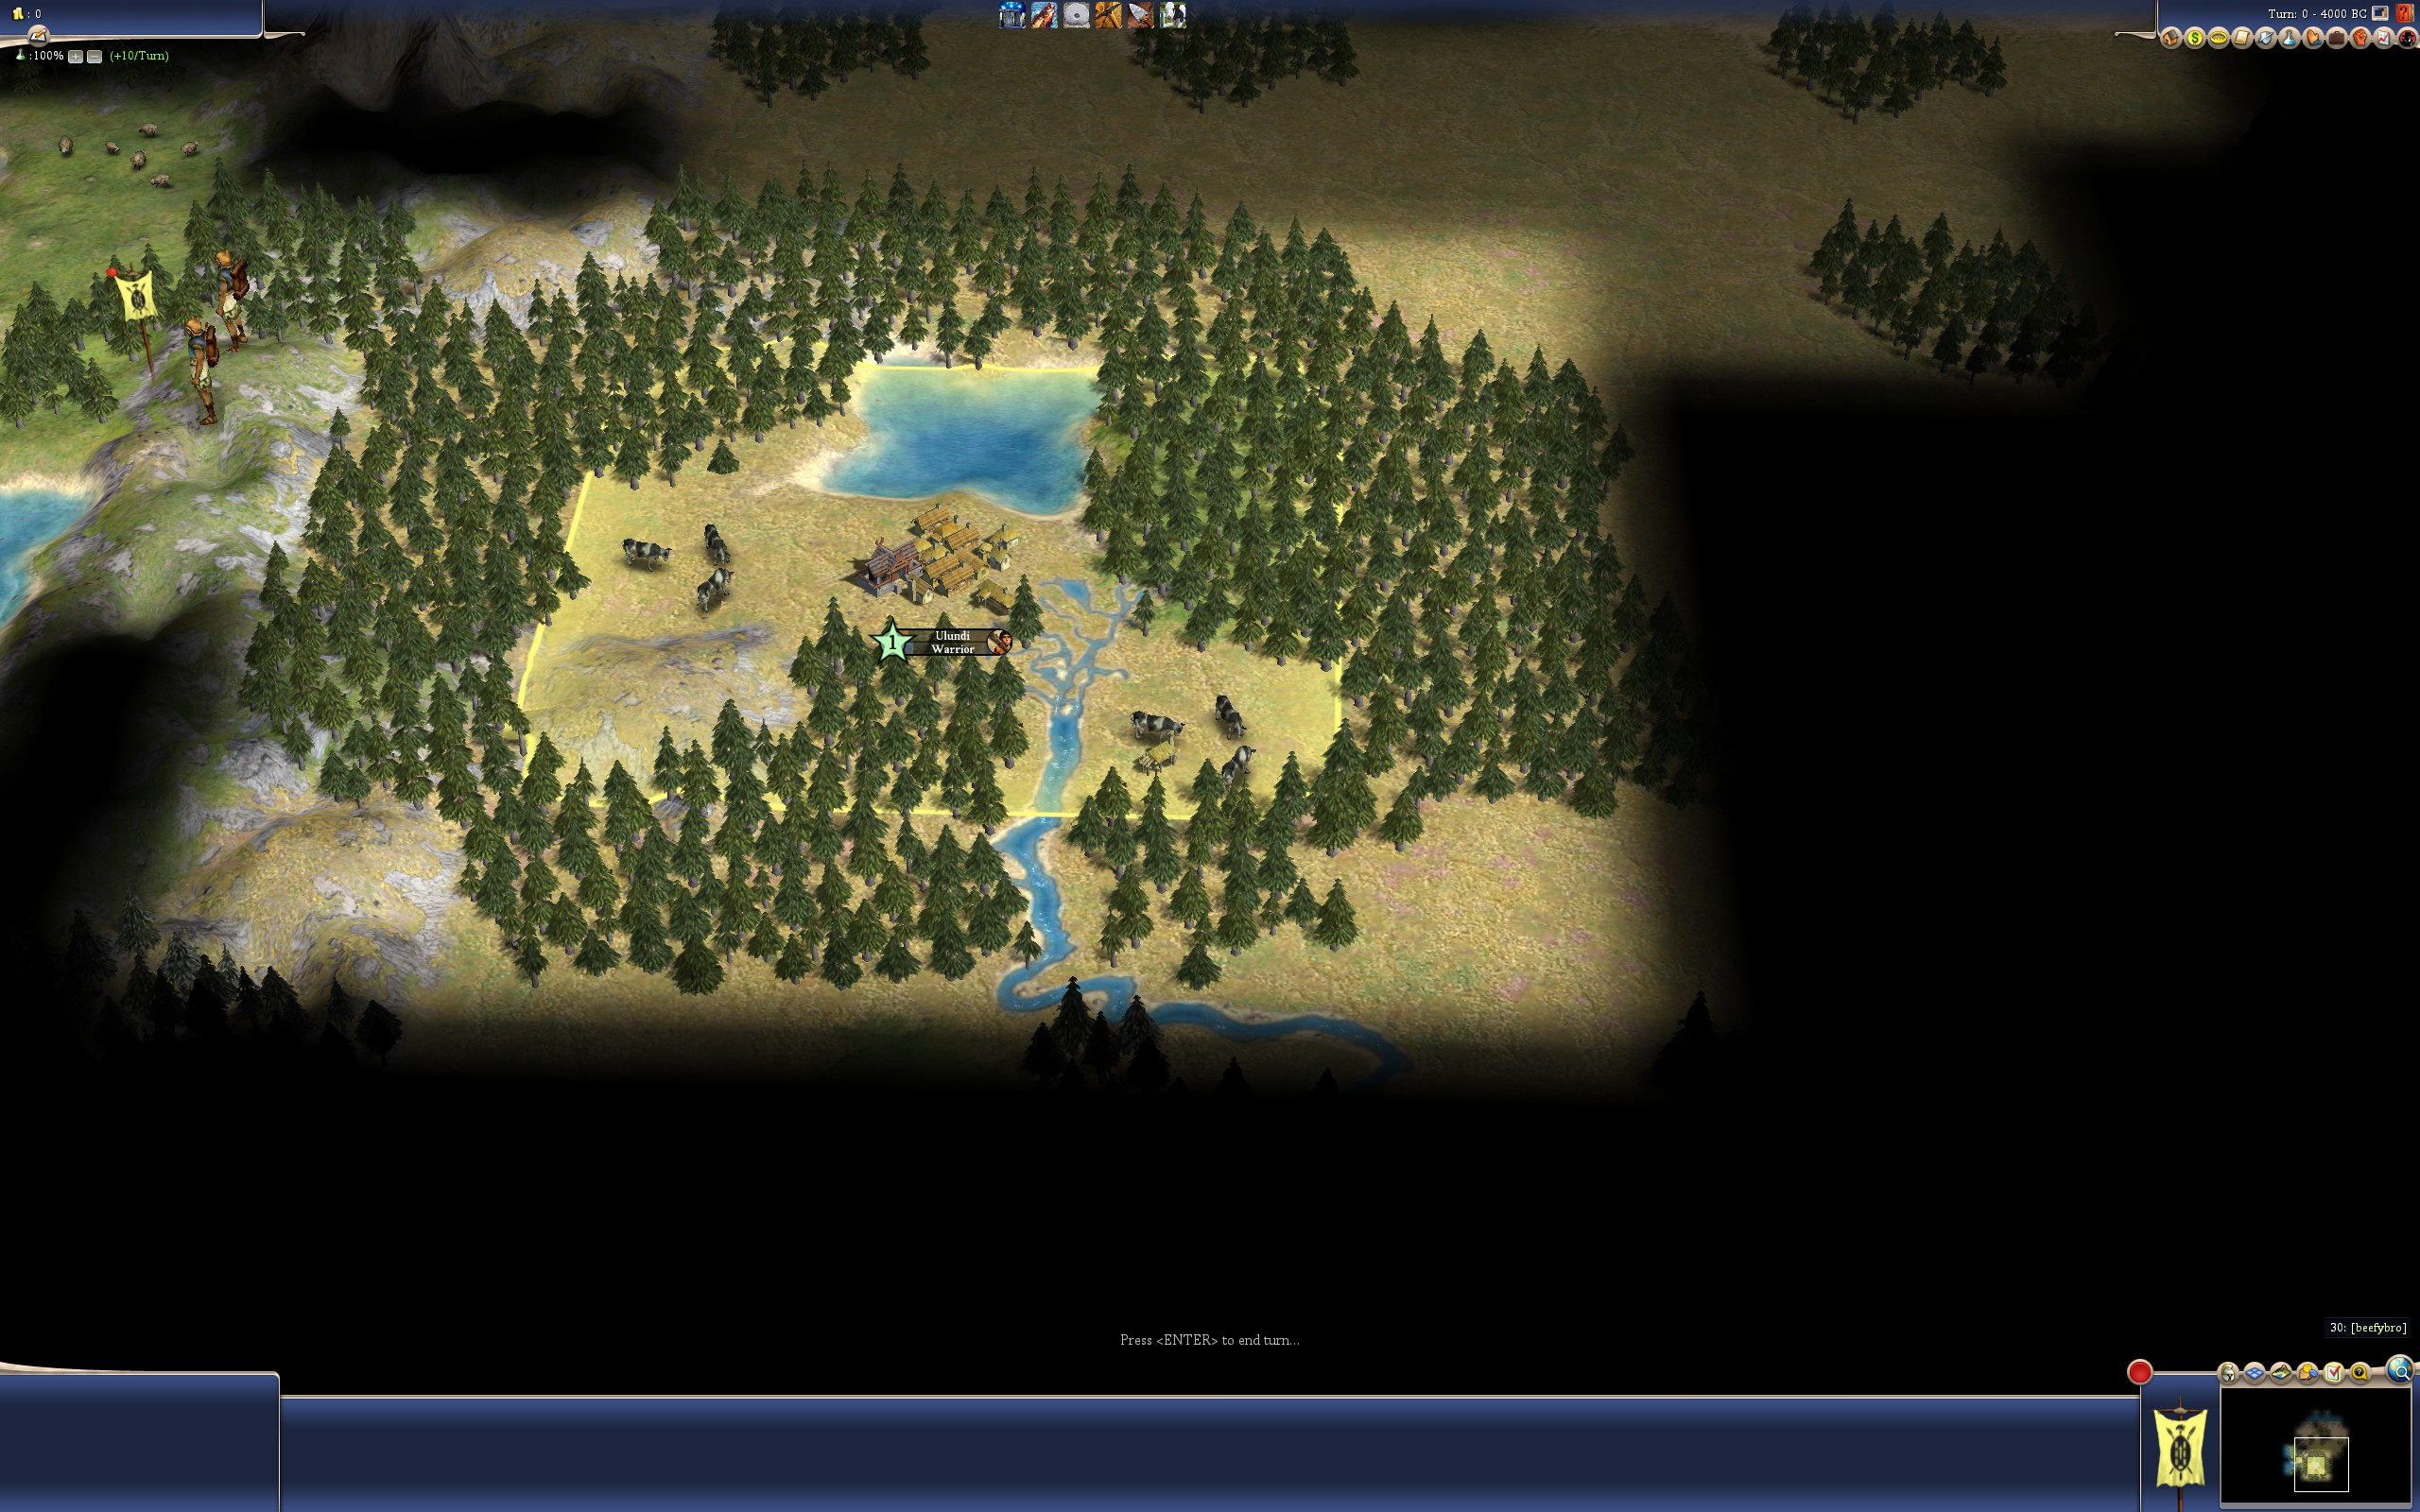
\includegraphics[width=1.0\textwidth]{1}

Capital looks pretty mediocre; I definitely like the density of forests, the river,
and the fact that it looks like I have viable expansion options in all directions.
Unforunately, the capital is clearly short on food which drastically reduces options.
The best I can probably hope for here is to turn this city into an OK production city.

My random civ turned out to be Zulu which is a pretty good one. Their uber building
(-20\% maintenance with barracks) and uber unit (2-move spearman) both come early
and are useful.

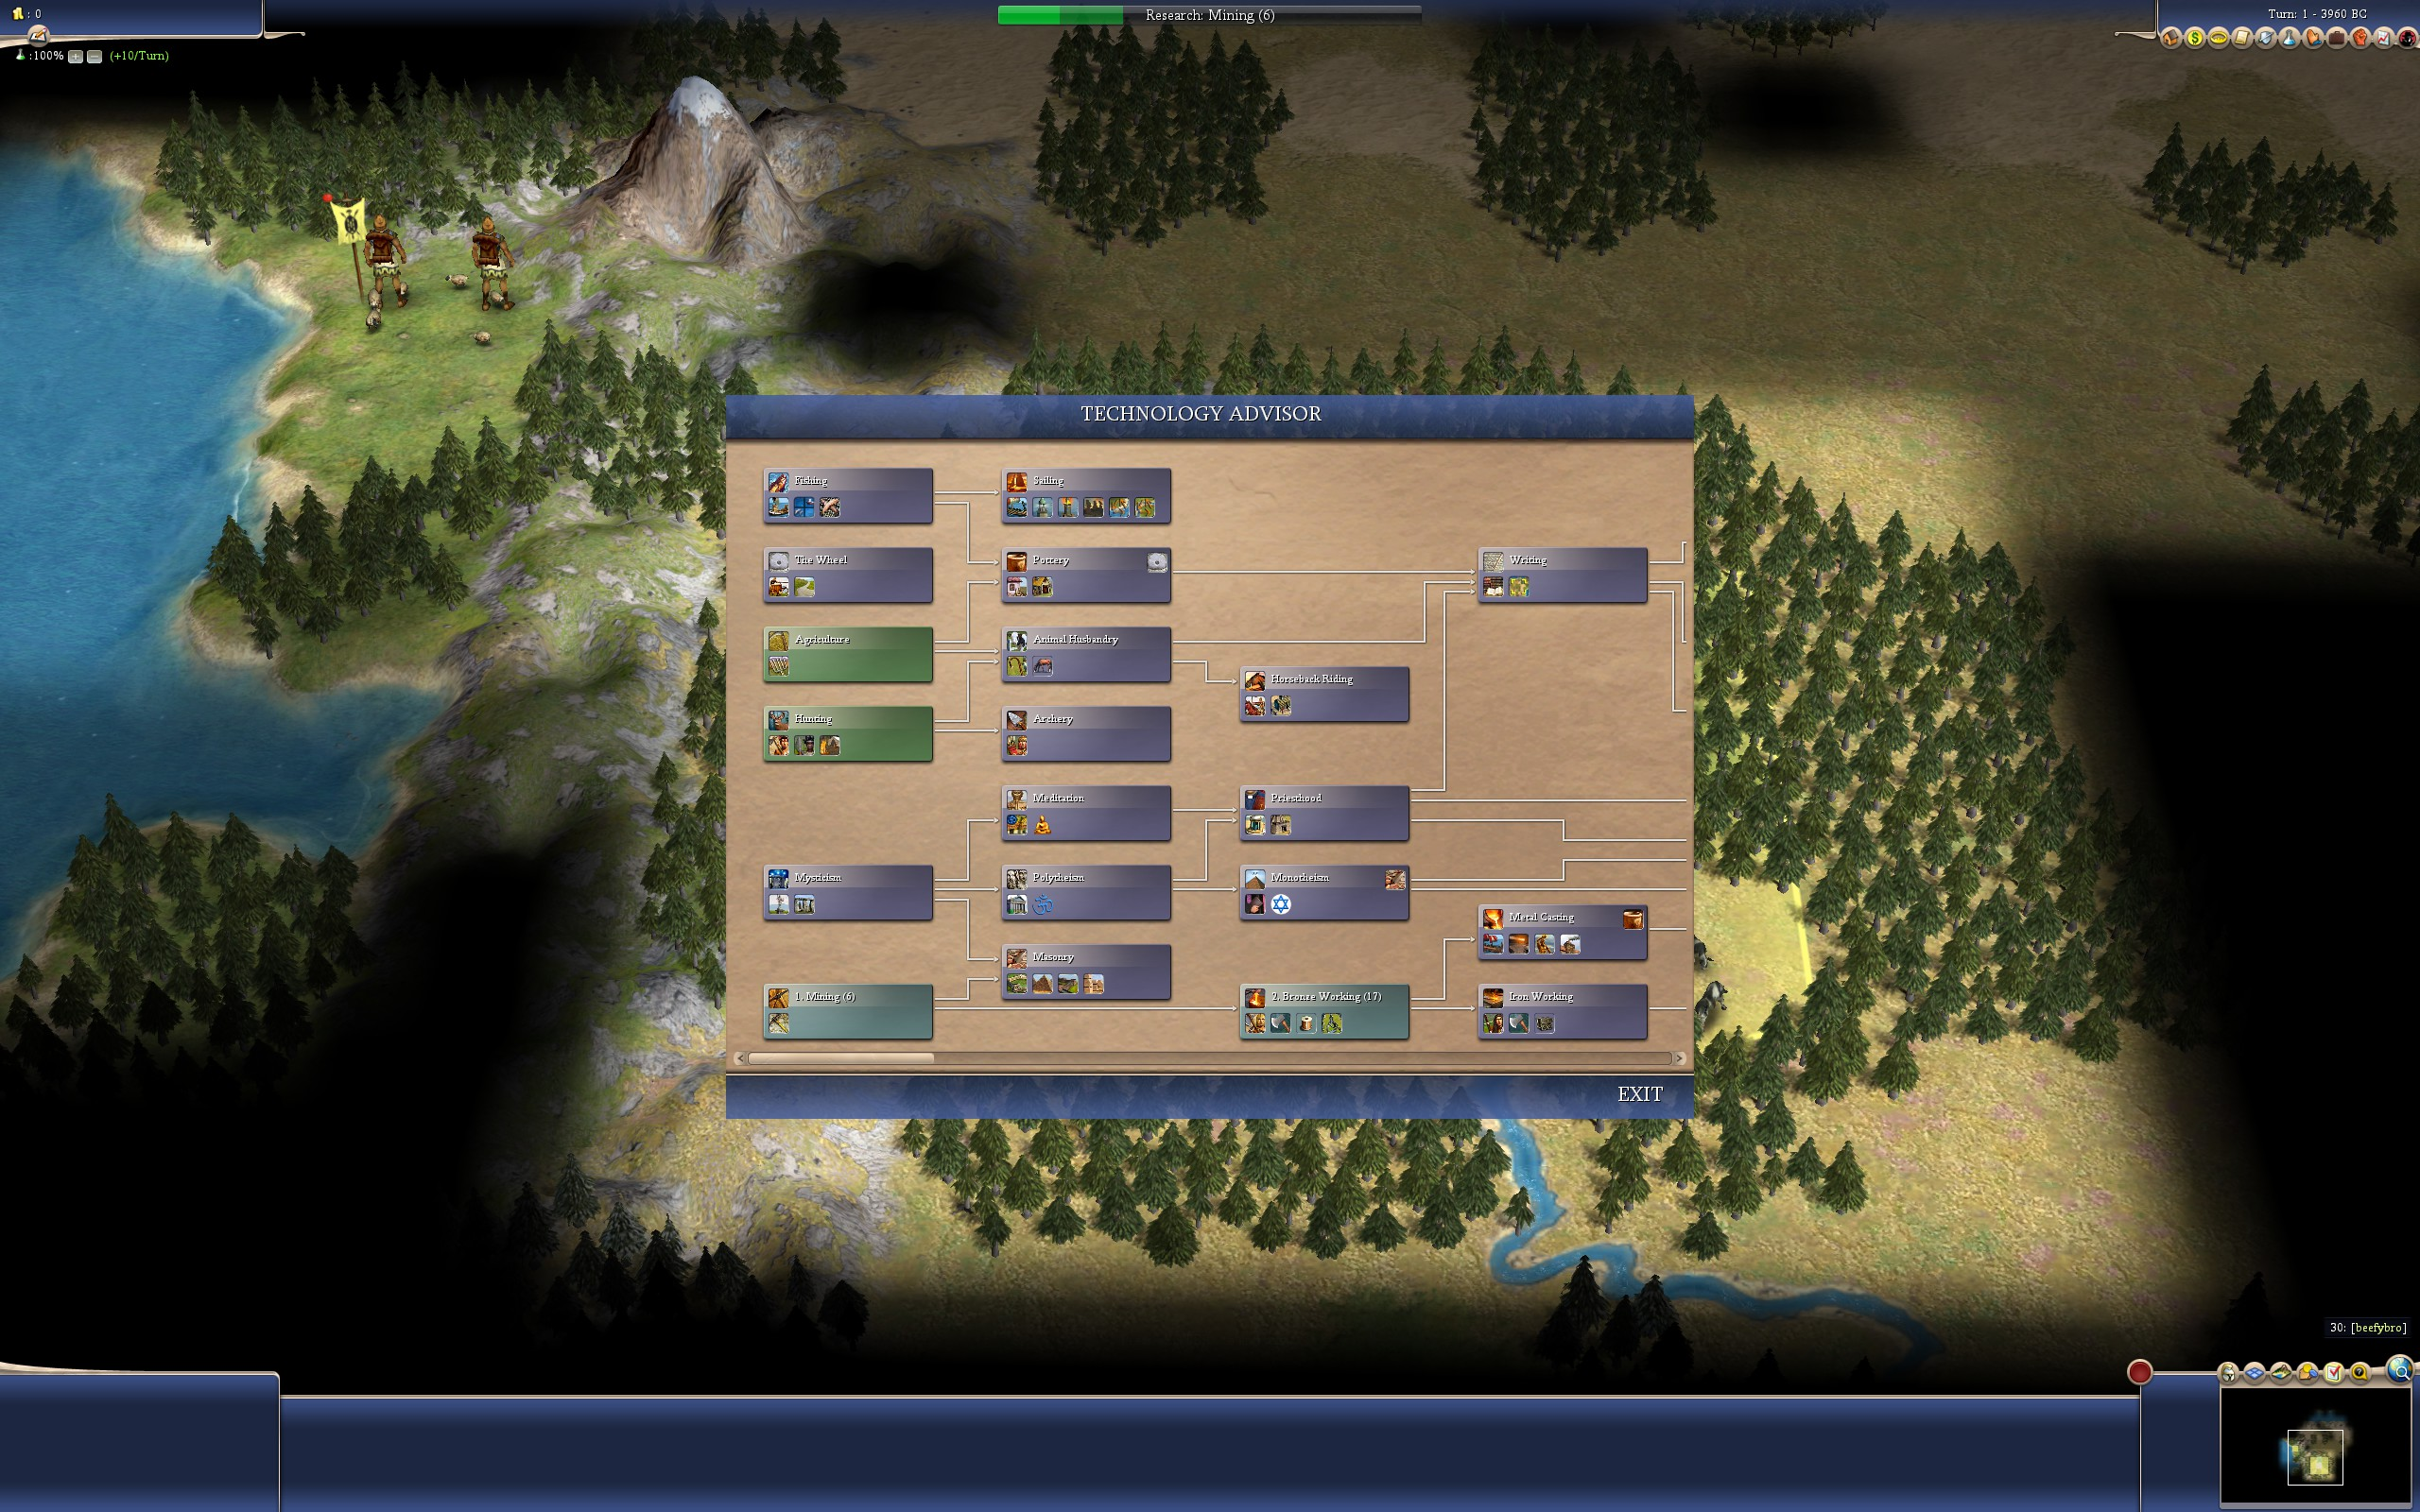
\includegraphics[width=1.0\textwidth]{2}

Here you see my bronze working (BW) beeline that I nearly always do. The Zulu do not start
with mining, so I have to research it first before I can get BW. This is why civs that start
with mining are slightly preferable. It will take a while to BW, so there's no point in making
a worker as he'll have nothing useful to do. Much better to make a warrior and let my cap grow
for a while.

Meanwhile, my scout in scouting in a rough circle around my cap as that's the most valuable
land for my to reveal since it will determine my expansion choices.

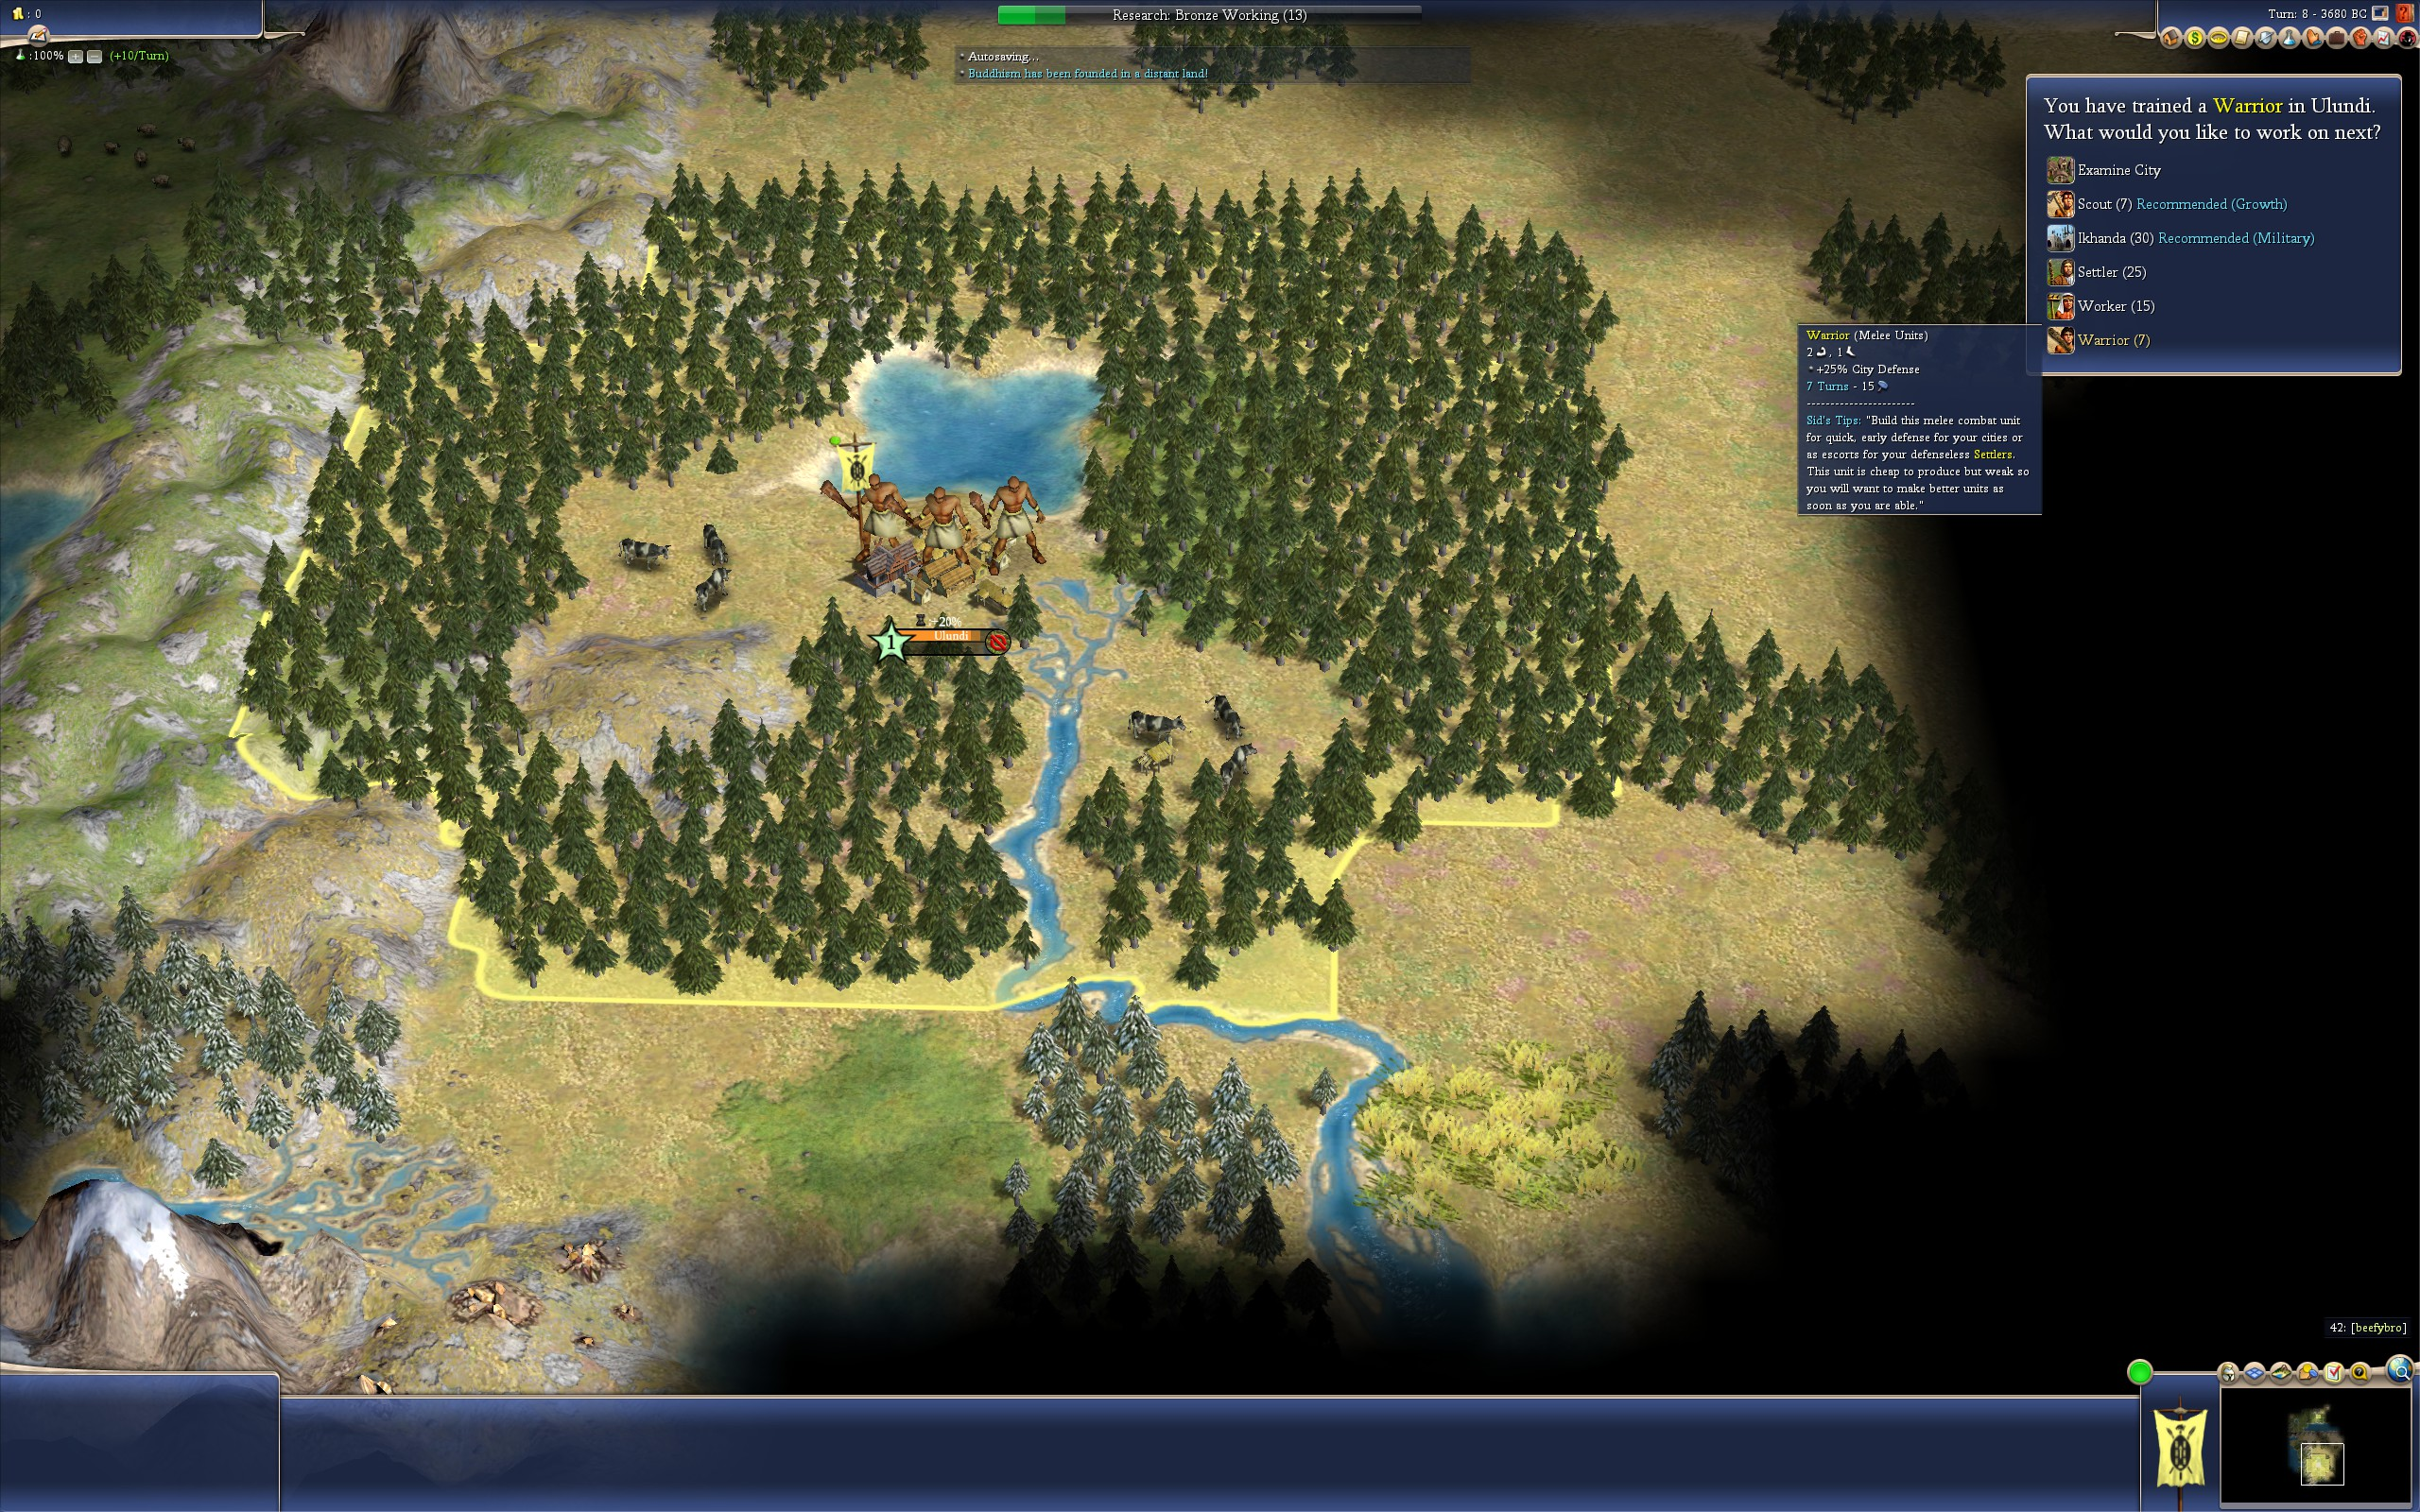
\includegraphics[width=1.0\textwidth]{3}

Couple things to note here. My cap finished a warrior and still is not size 2; this means I need
to partial-build a warrior until my cap has grown and then switch to worker. The other noteworthy
item is the gold to my south. Working a gold tile can singlehandedly double your early game GNP
and greatly help to finance expansion. It's looking like I'm in a great plains type area which is
common in tectonic lakes. This means my land will be mediocre and that rexing is my best option
(compensate for mediocre land quality by gaining a large quantity).

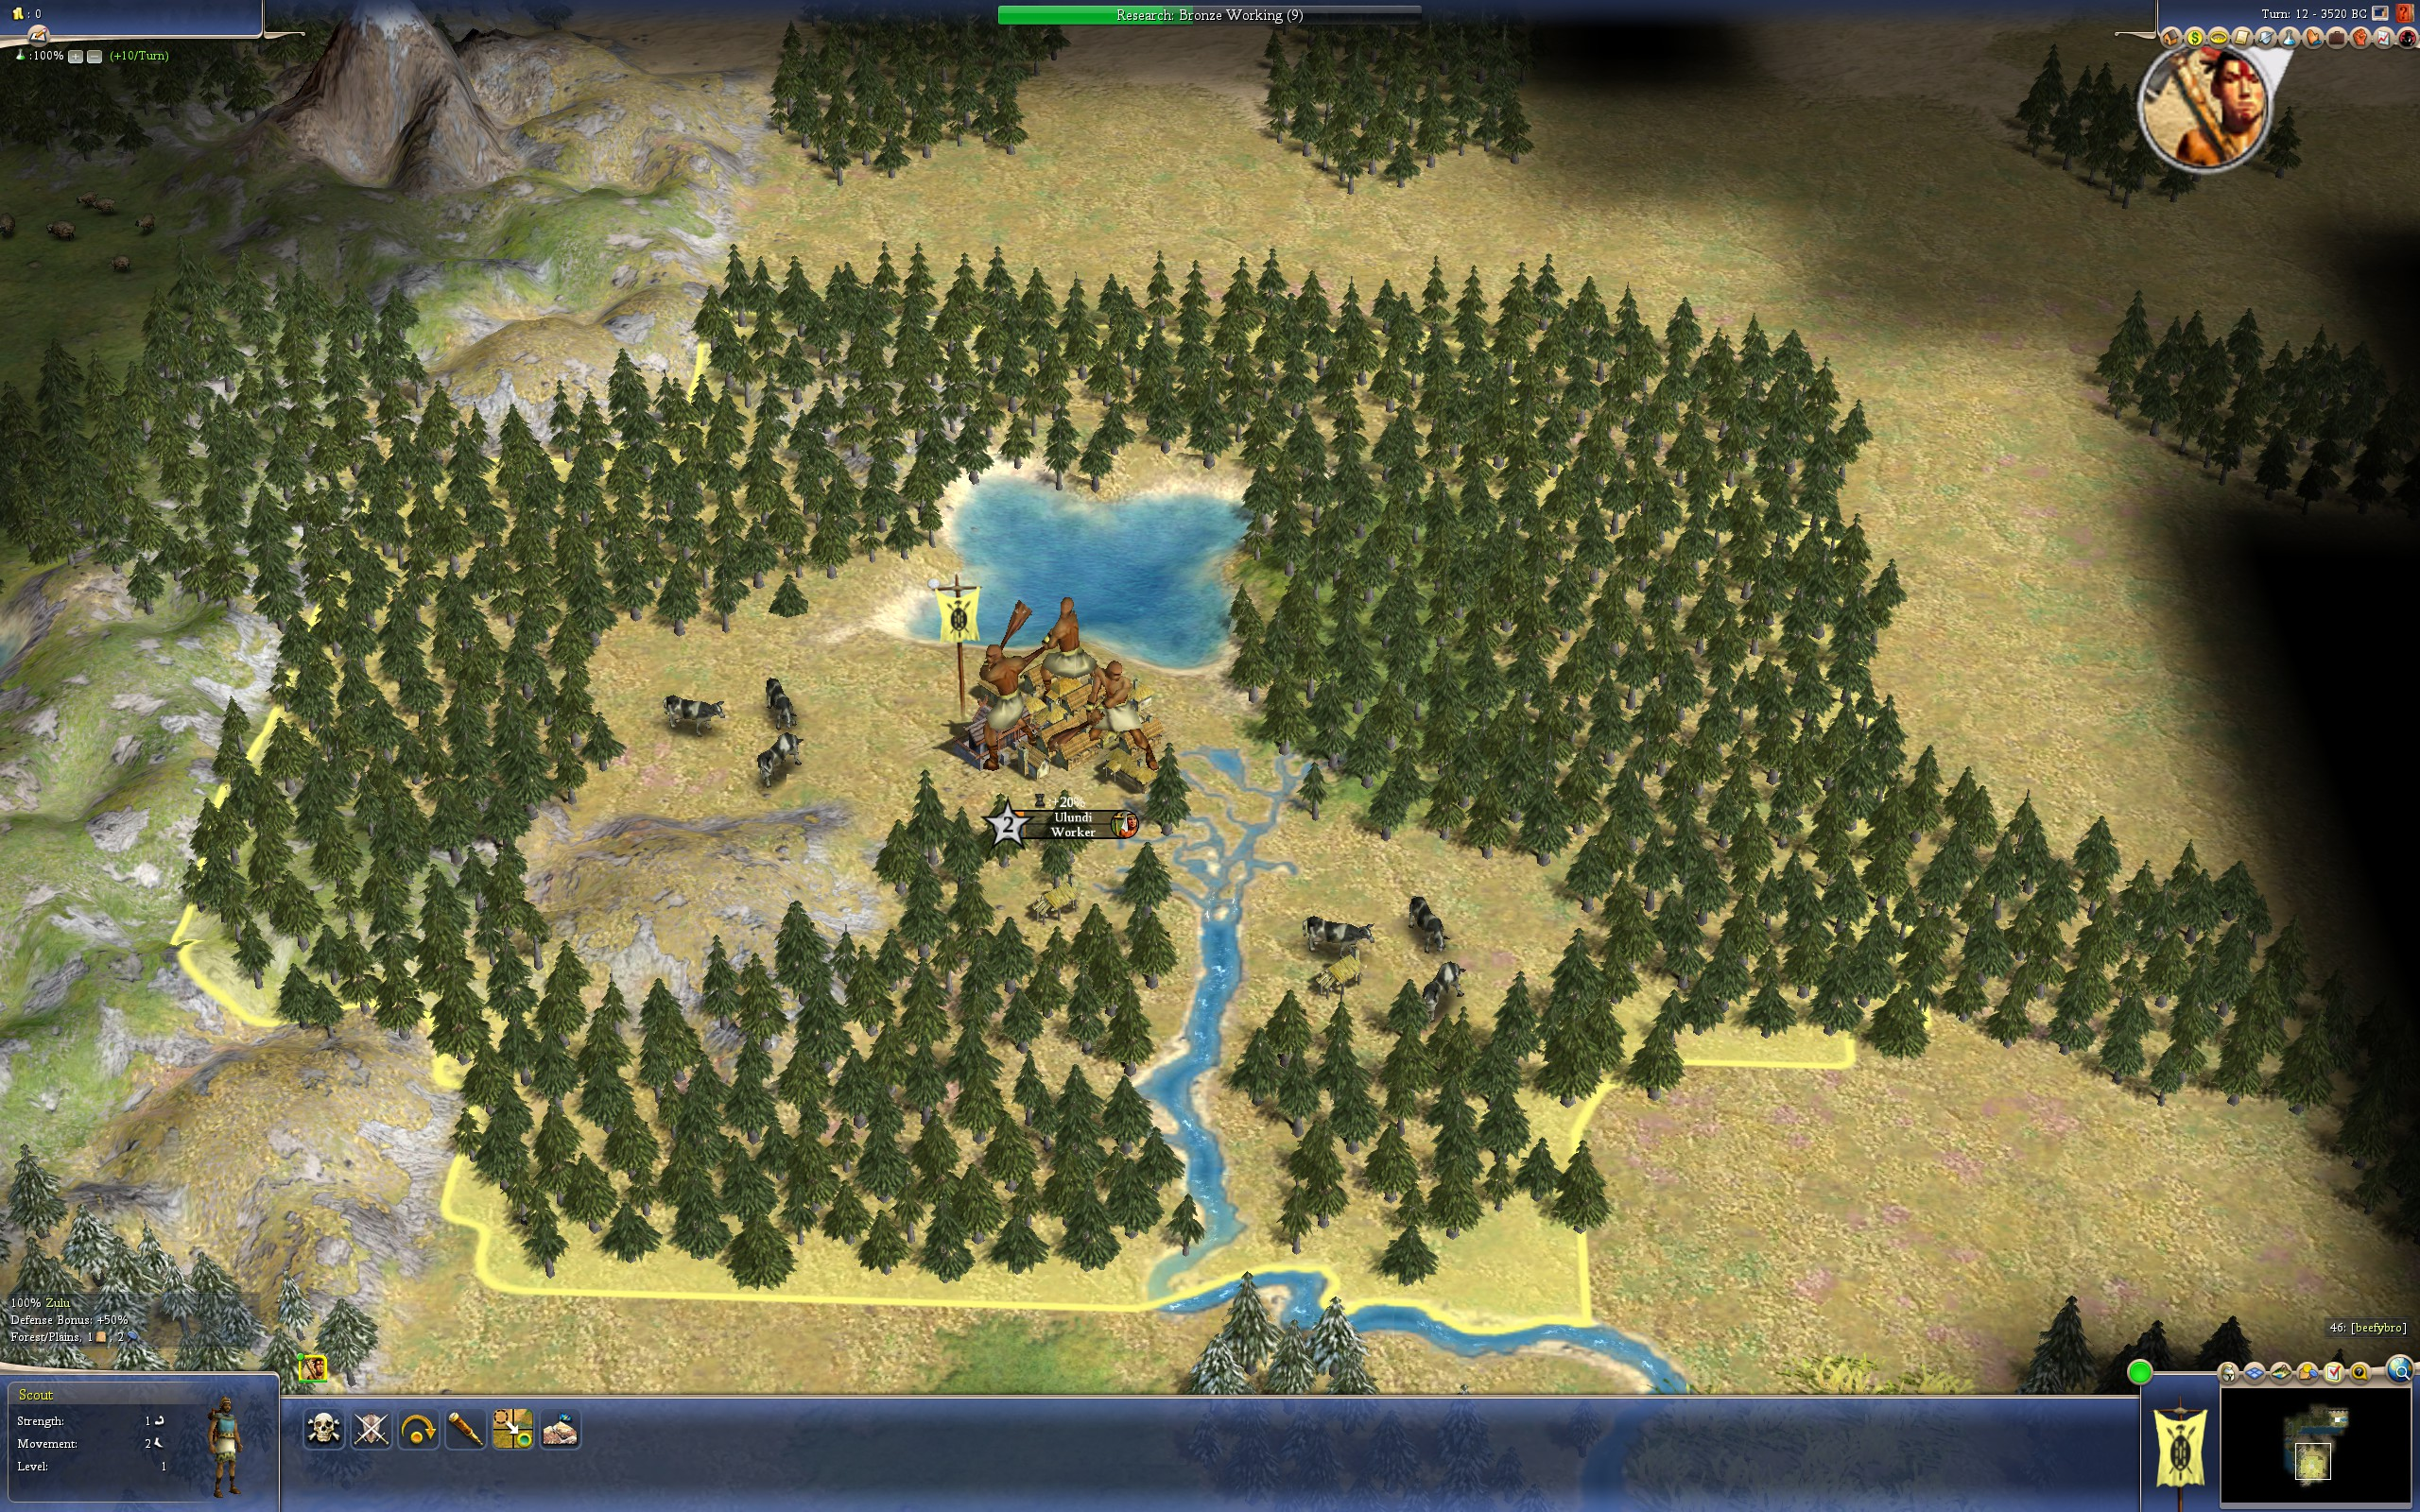
\includegraphics[width=1.0\textwidth]{4}

Here you see I've switched to worker the instant my cap hit size two even though the warrior
I was making is not complete. You want you first worker to pop out as soon as BW arrives so
that you can take advantage of the games most powerful early-game mechanic, chopping, as soon
as possible.

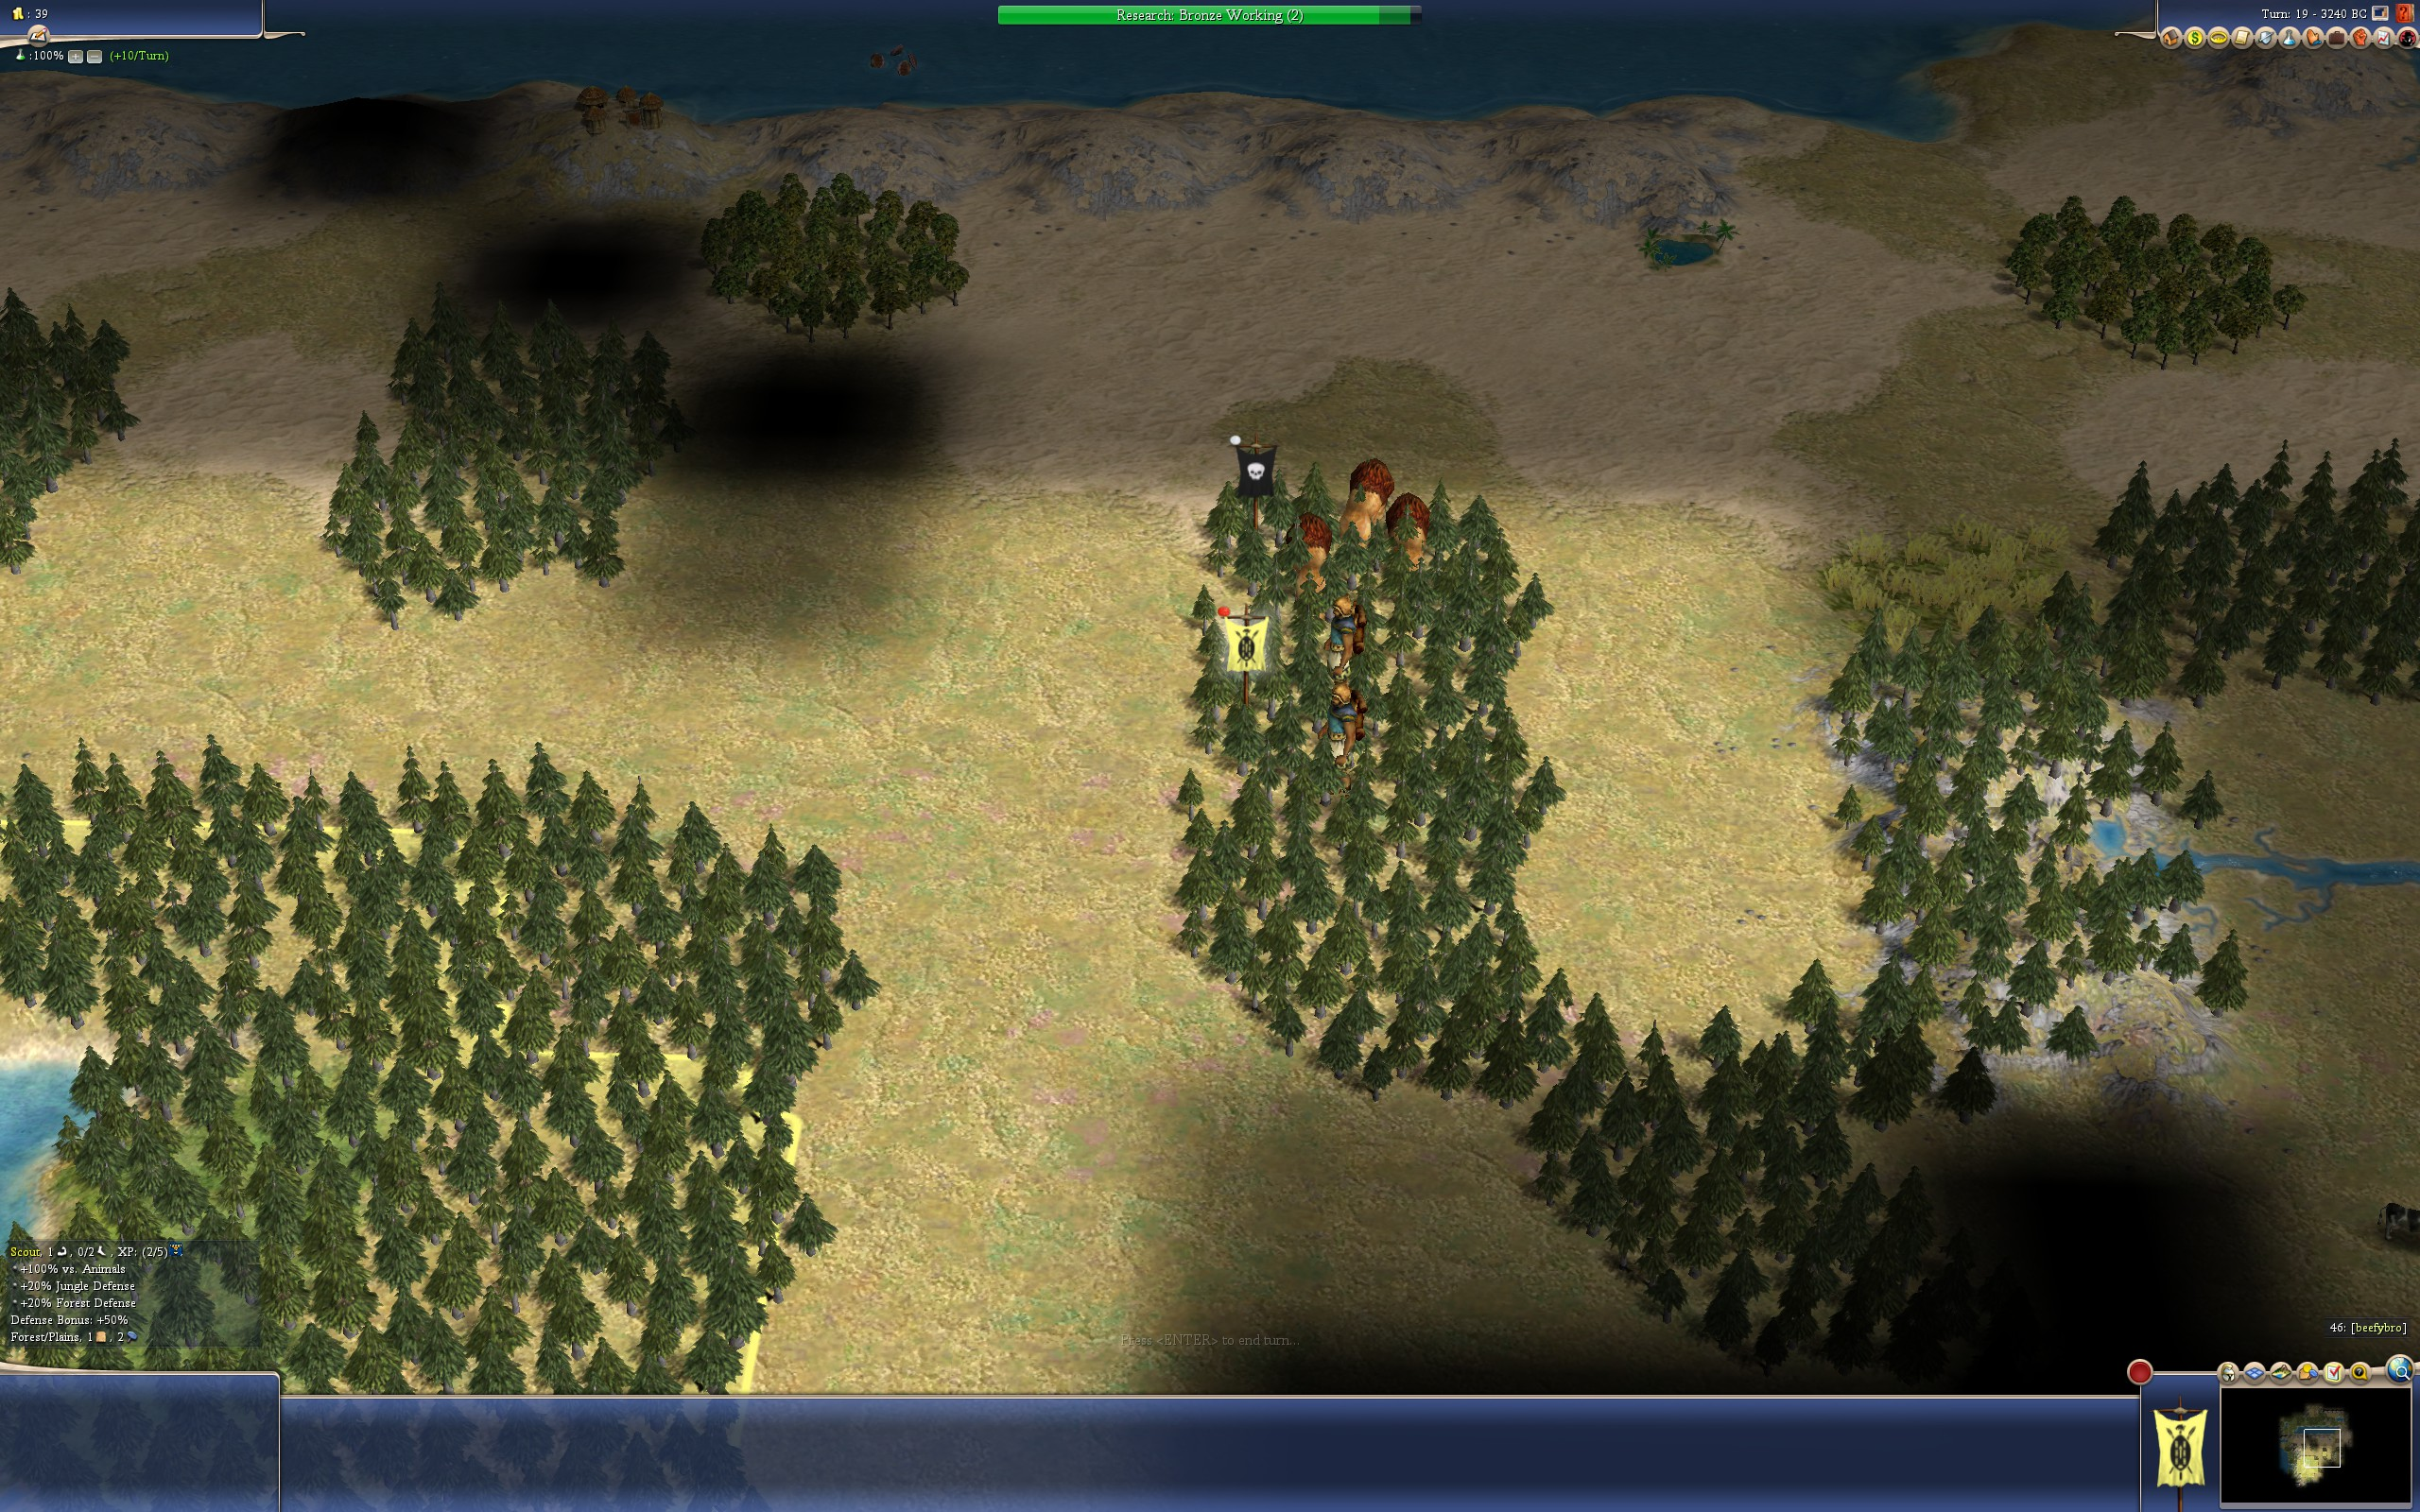
\includegraphics[width=1.0\textwidth]{5}

I included this image to demonstrate scout/explorer micro which is a useful skill in the early
game. The idea is to bait animals into attacking your scout when he's on a strong defensive
tile (forests). You then promo your scout with the woodsman promo (forests tend to be
much more common than hills. You then try to leave your scout in forested tiles when you end turn.
This maximizes his chance of surviving. If you're lucky enough to get a second promo, woodsman II
provides double move speed through forest/jungle which helps your scouting immensely. If you can keep
your scout alive, you'll reveal more terrain earlier and get more goody huts, both great things for your civ.

In this image, I spotted the lion from a far and then positioned my scout in the forest next
to him deliberately. Much like Pat after losing a wonder city, animals can almost always be counted on
to lash-out blindly at the nearest unit they see, even if their combat odds are terrible. This will produce
a near-certain victory for my scout, and therefore another exp point and will remove a potential threat
to him as he moves away from the forest.

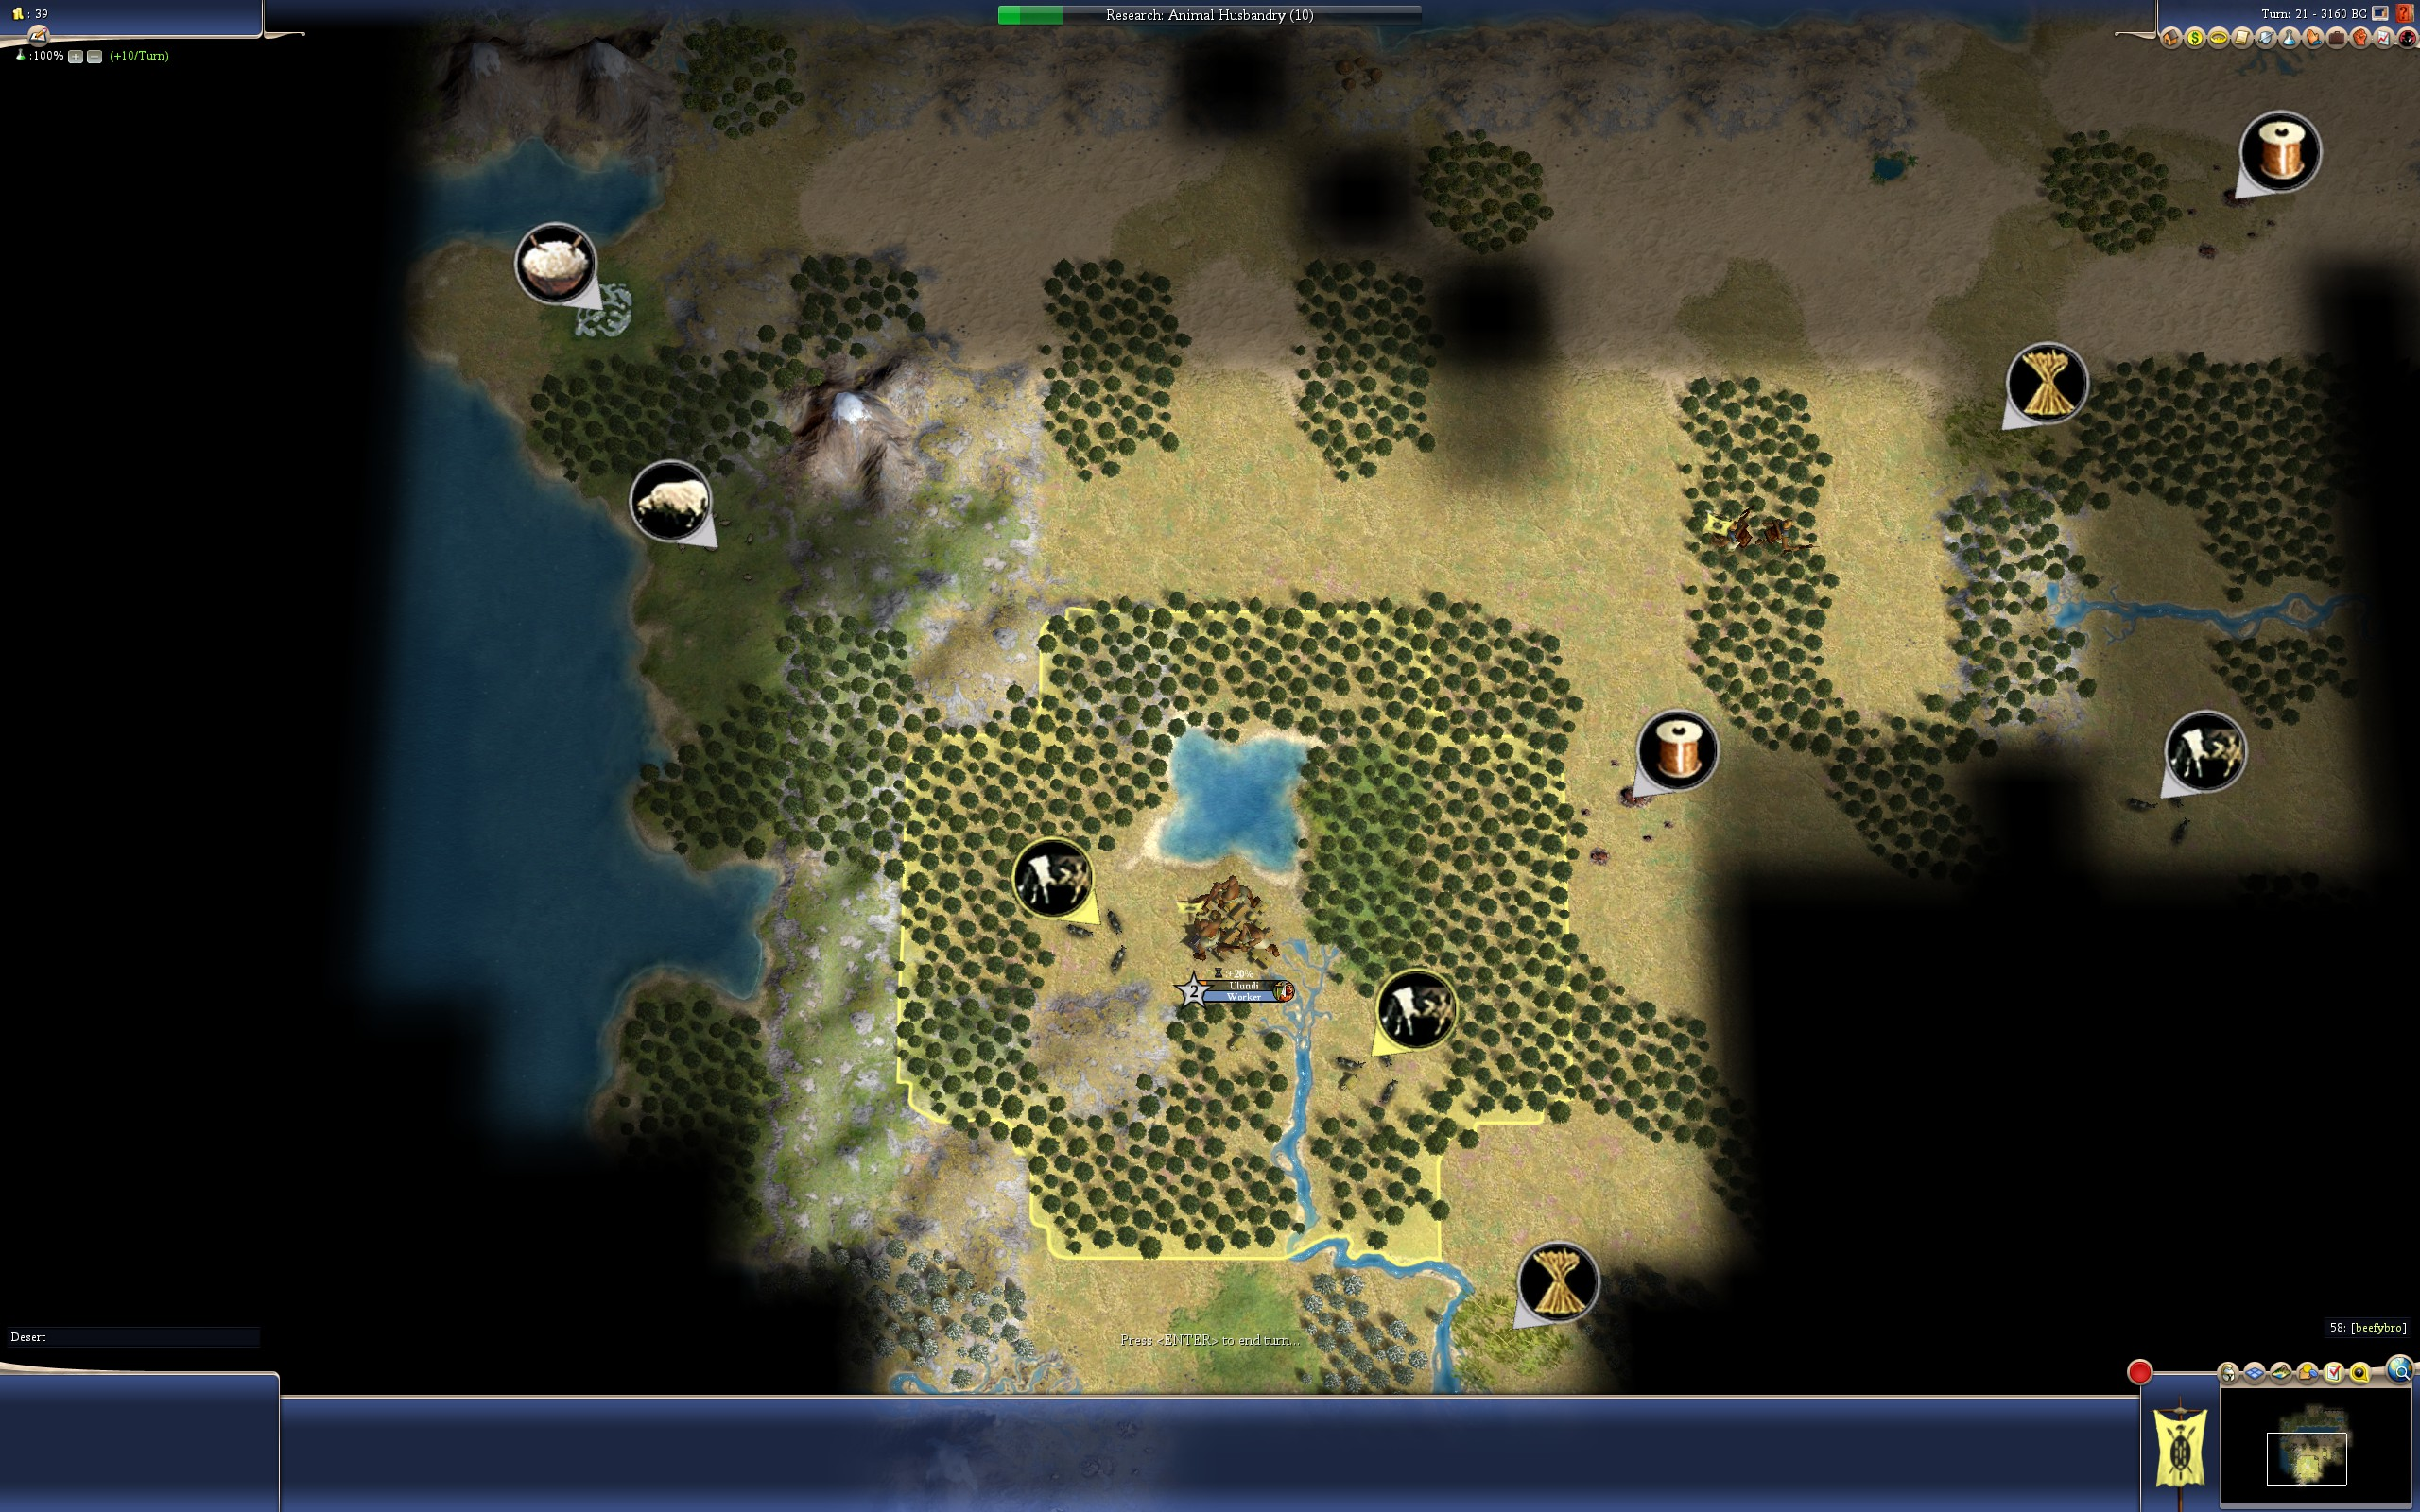
\includegraphics[width=1.0\textwidth]{7}

Here's a lay of the land. The river to my east has some food nodes near it, so that could make for
decent cities. I also have a nearby bronze which is excellent. That should be top priority after getting
that gold to the south online. You can see that I'm going for Animal Husbandry (AH) after getting BW, which is a
no brainer since my capital has two animals in its BFC.

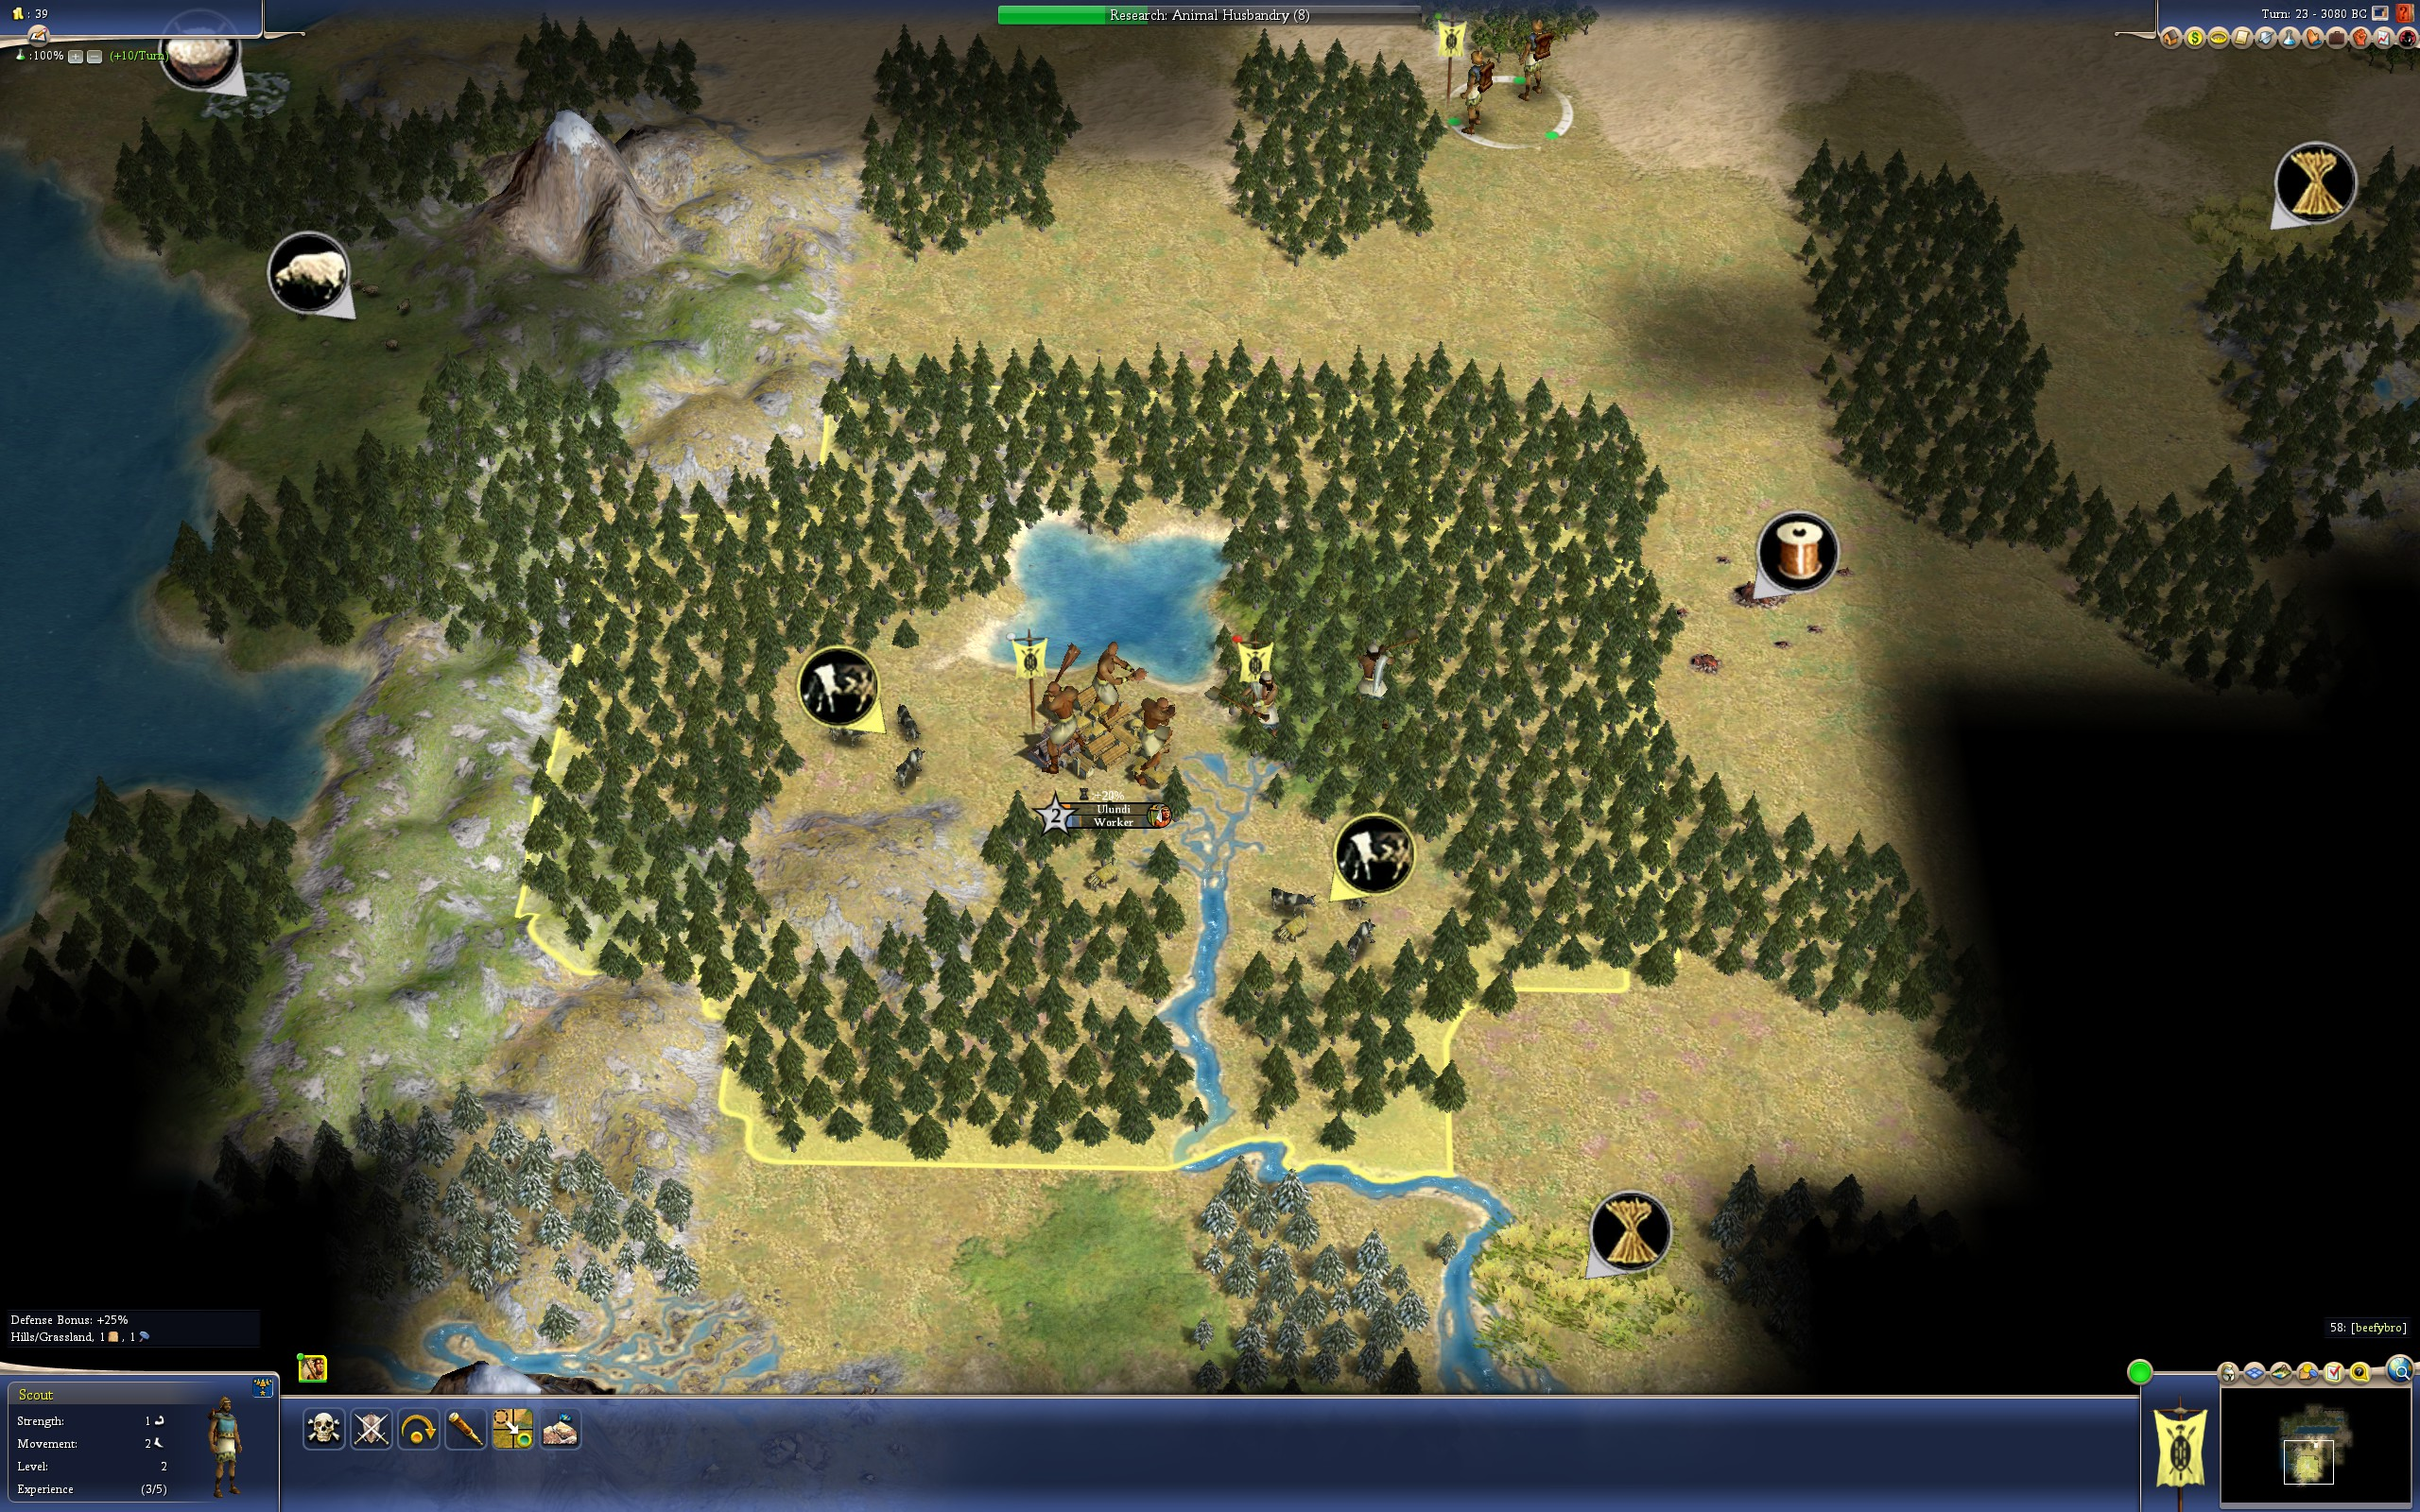
\includegraphics[width=1.0\textwidth]{8}

My worker is complete and he's moving to chop some forests. I immediately start a second worker. The
idea here is the one worker will be a chop-machine and the other will start to improve the tiles in my
capital. You don't have to play it this way, but it's the opener I almost always prefer.

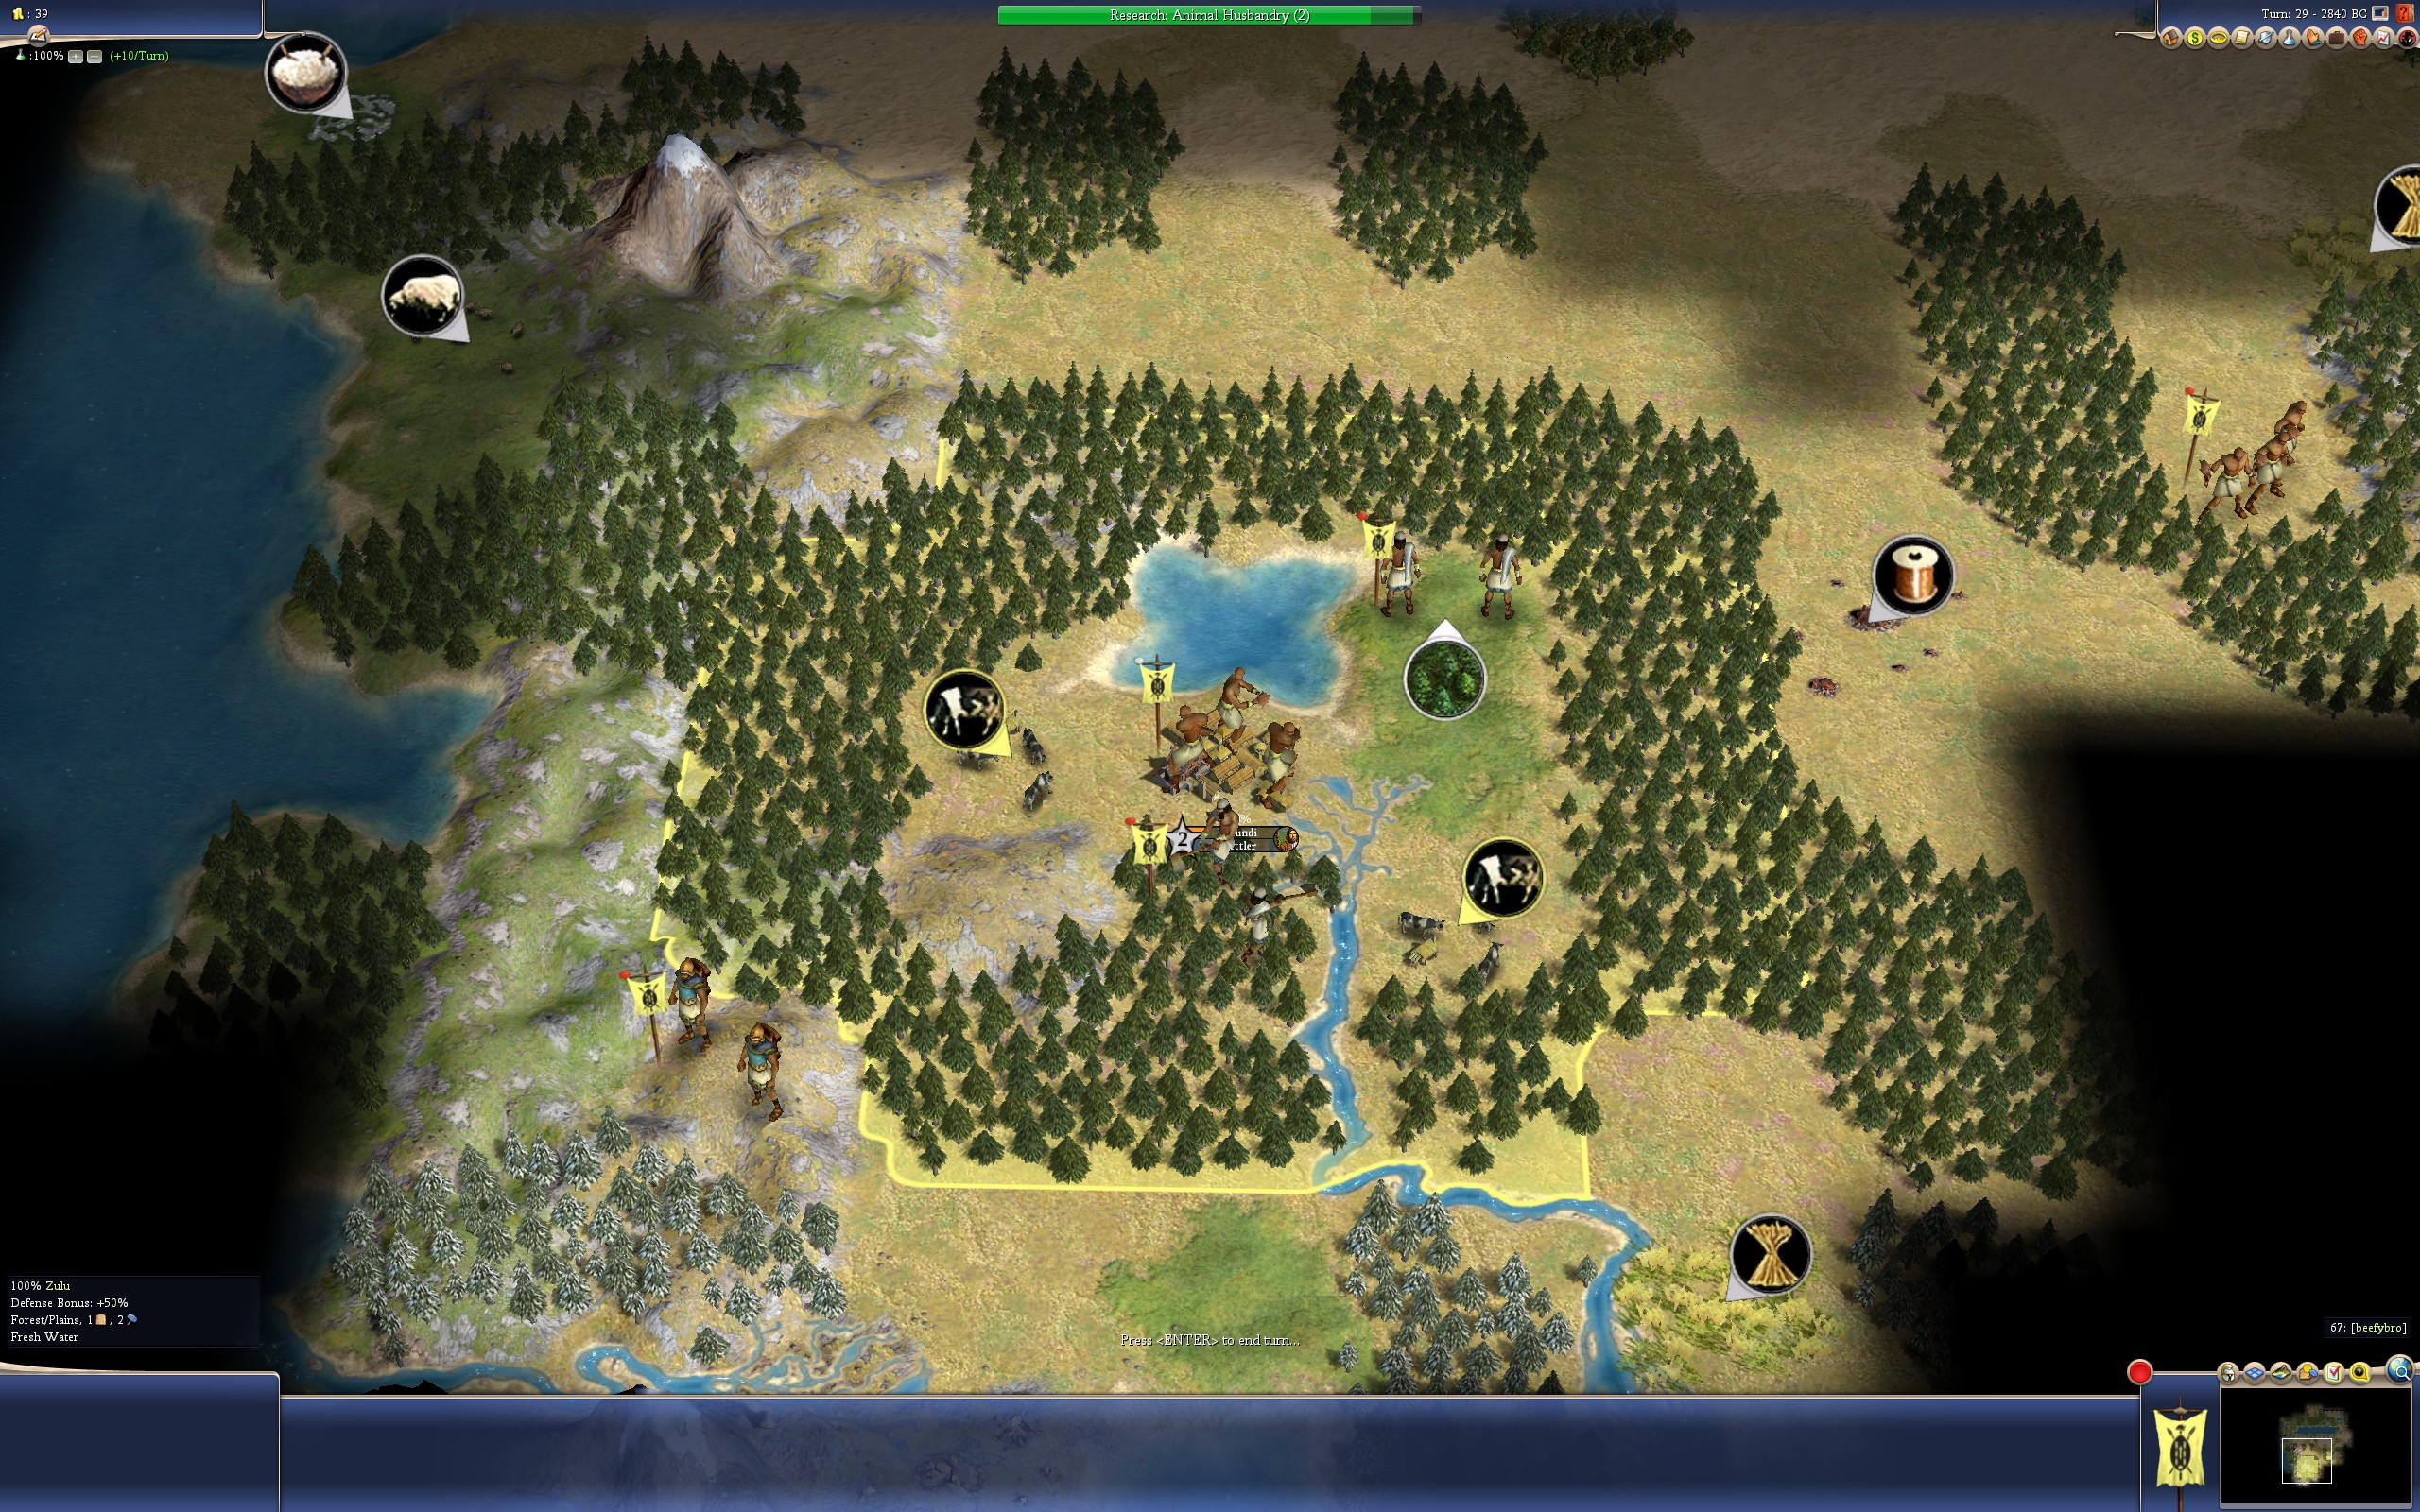
\includegraphics[width=1.0\textwidth]{9}

My second worker has popped and I briefly have two choppers. AH is not quite done yet,
so the only useful thing the second worker can do is chop. My second warrior you see to the east was gained
from a hut, which is quite nice. It means my first settler already has an escort, so I start making him
immediately.

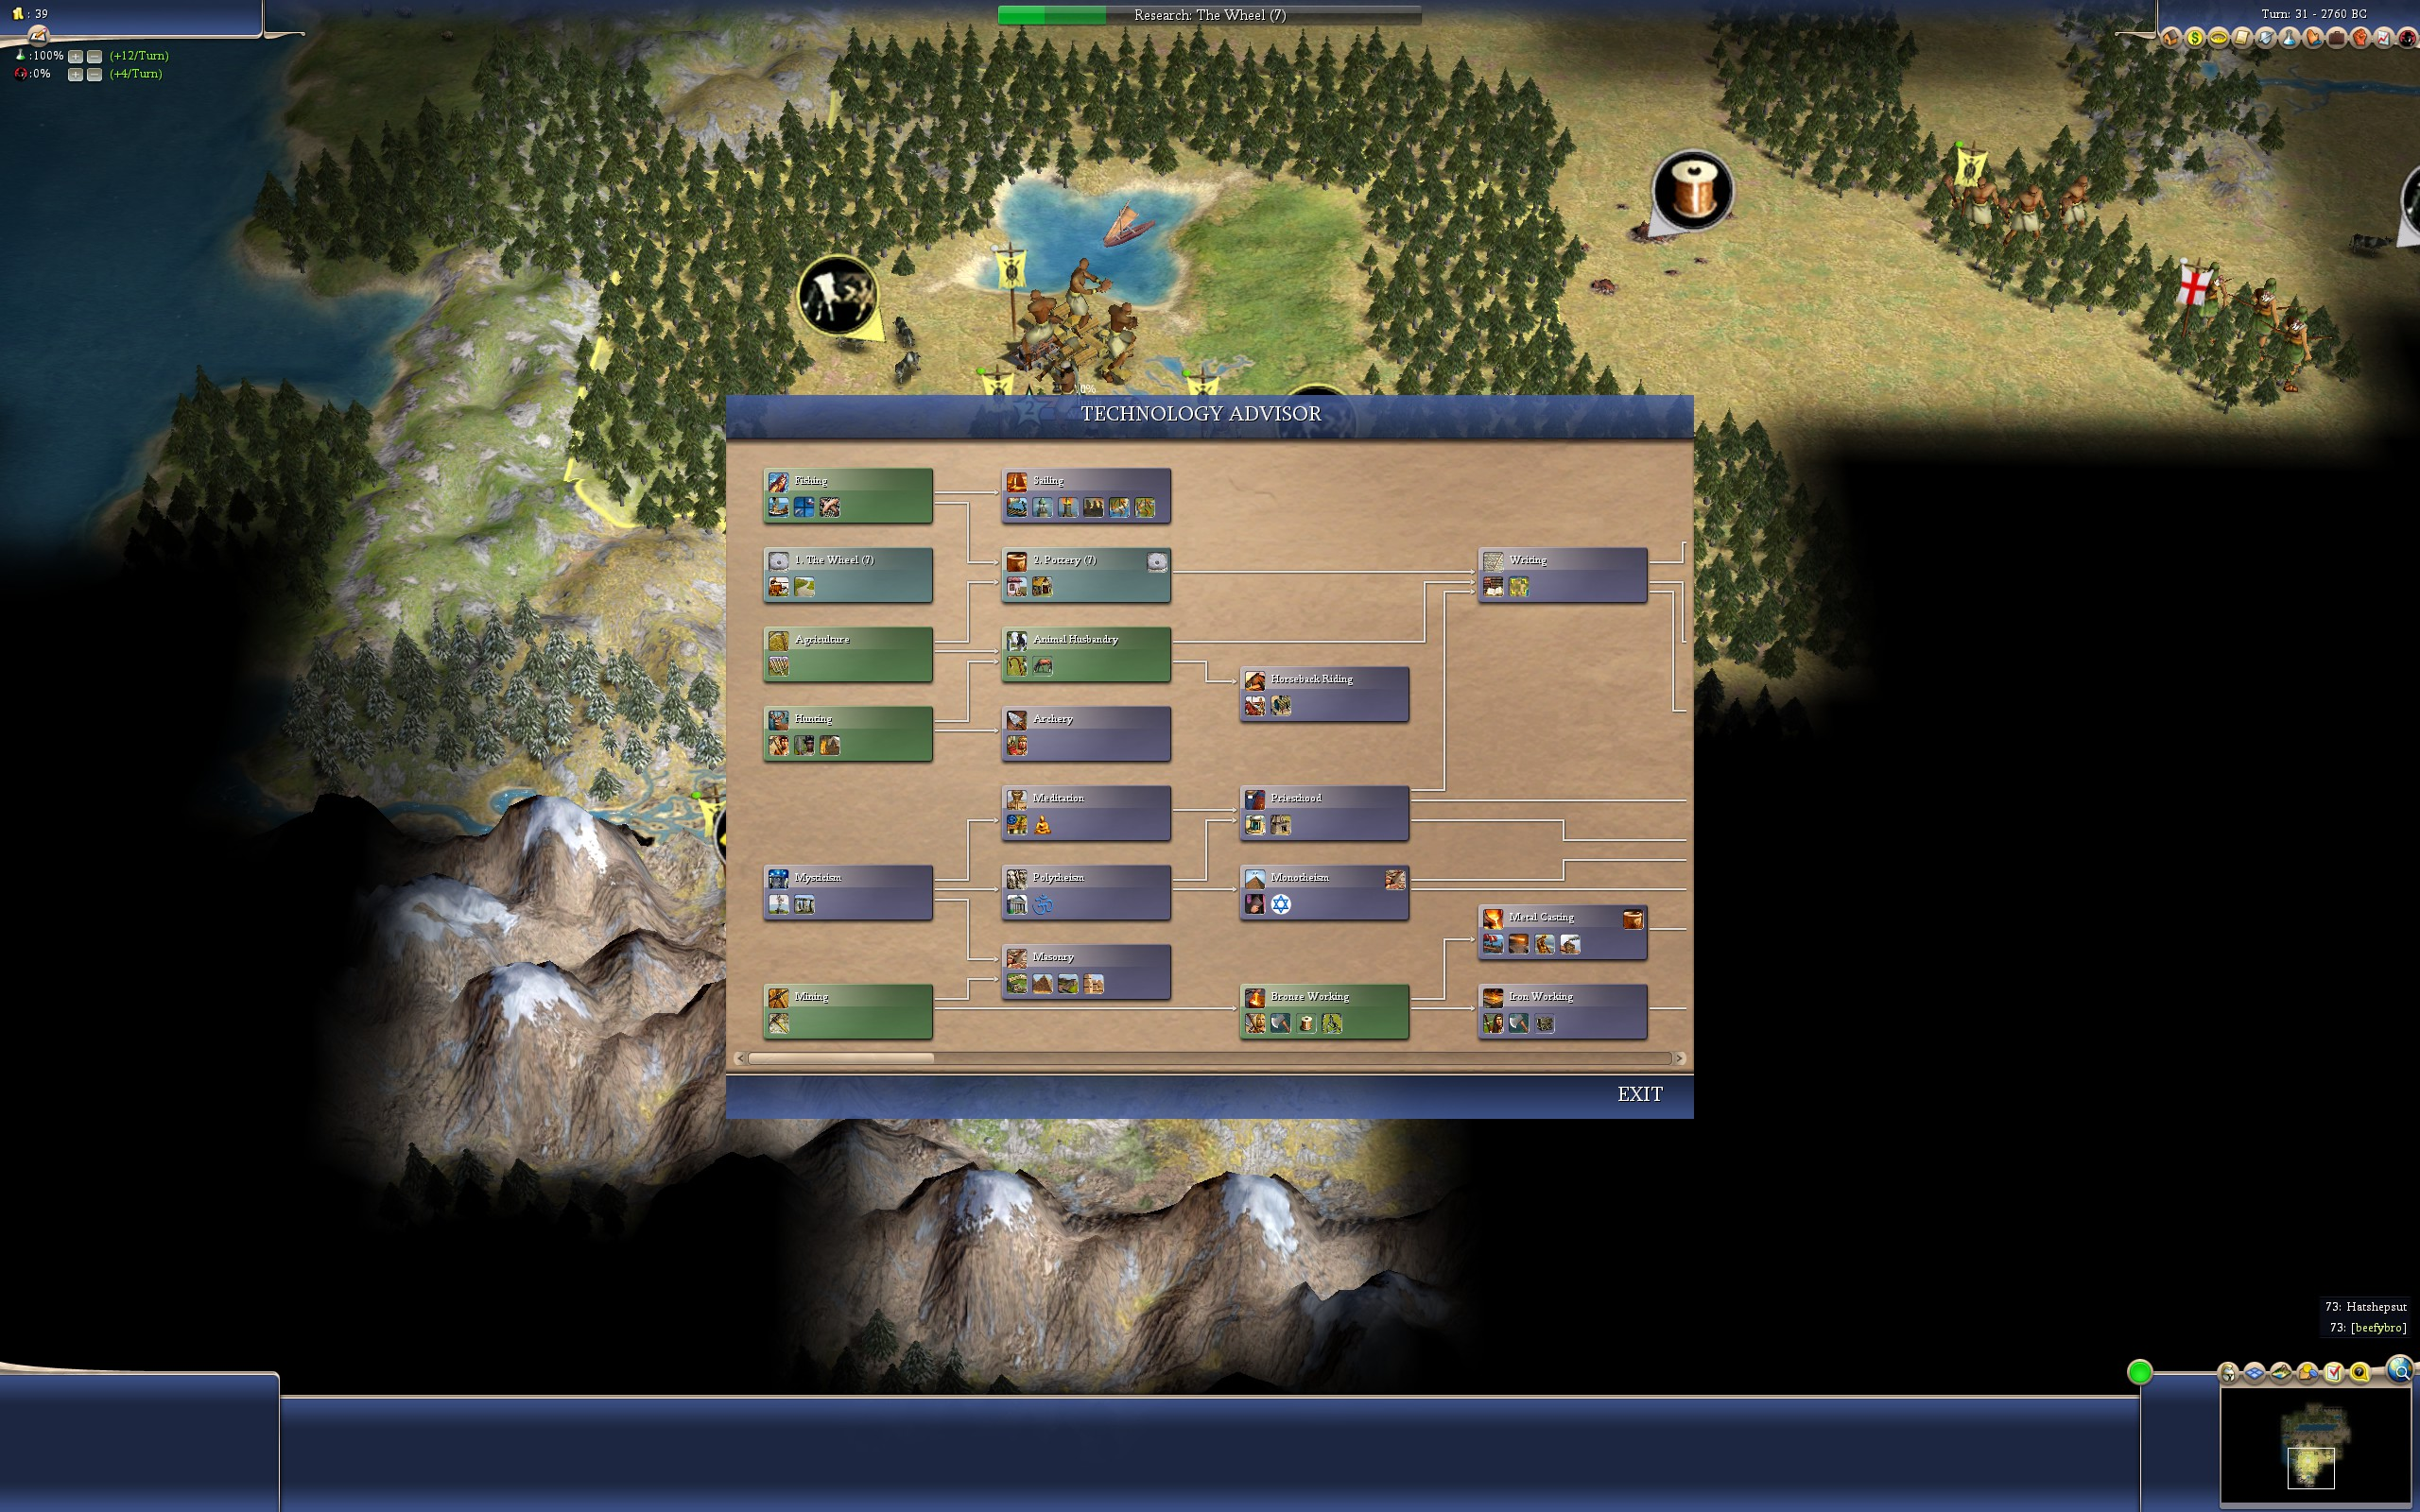
\includegraphics[width=1.0\textwidth]{11}

AH is done and it's time to pick some new techs to research. Wheel going to Pottery is the obvious choice here.
Roads, cottages, and granaries are all extremely useful. The only time I would not go this route is if I still
lacked a tech needed to improve a bonus tile in my capital or I was beelining for a religion or early game wonder.

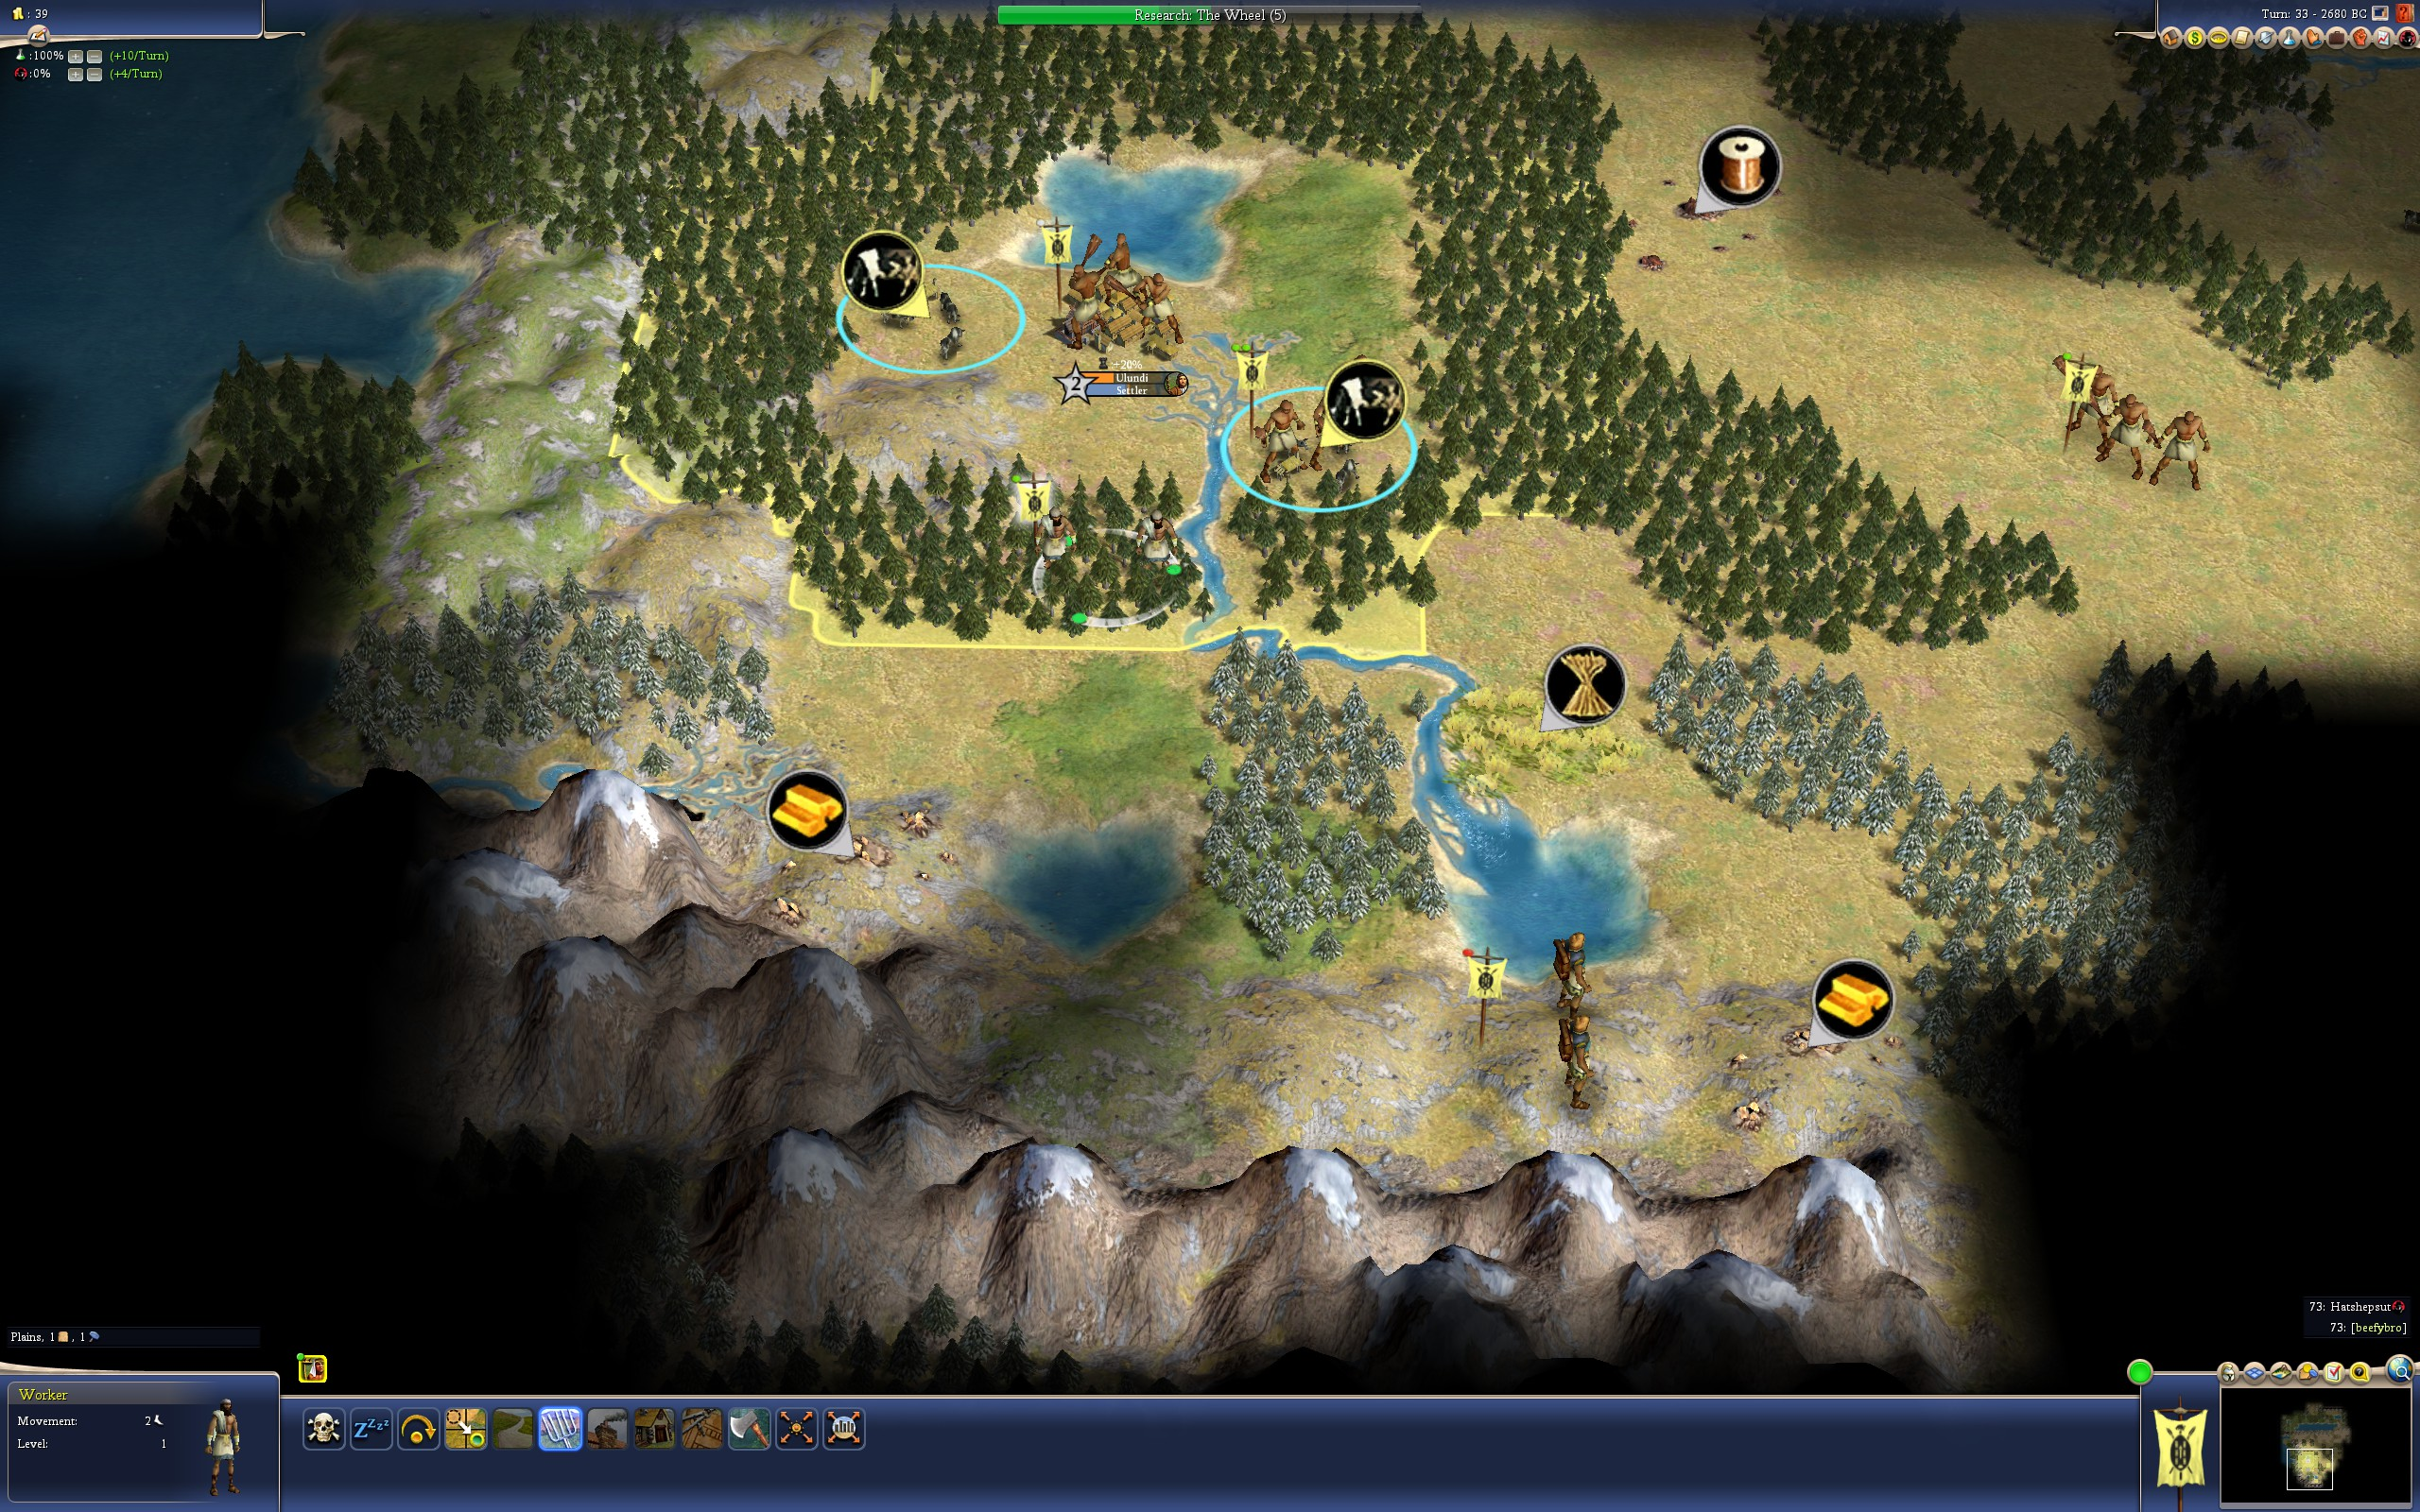
\includegraphics[width=1.0\textwidth]{12}

My scout has revealed a second gold node! And it's even reachable from the same city spot (1 tile NW of
current scout position) as the one that picks up the first gold. This is a game changer and is my civ's
top priority.

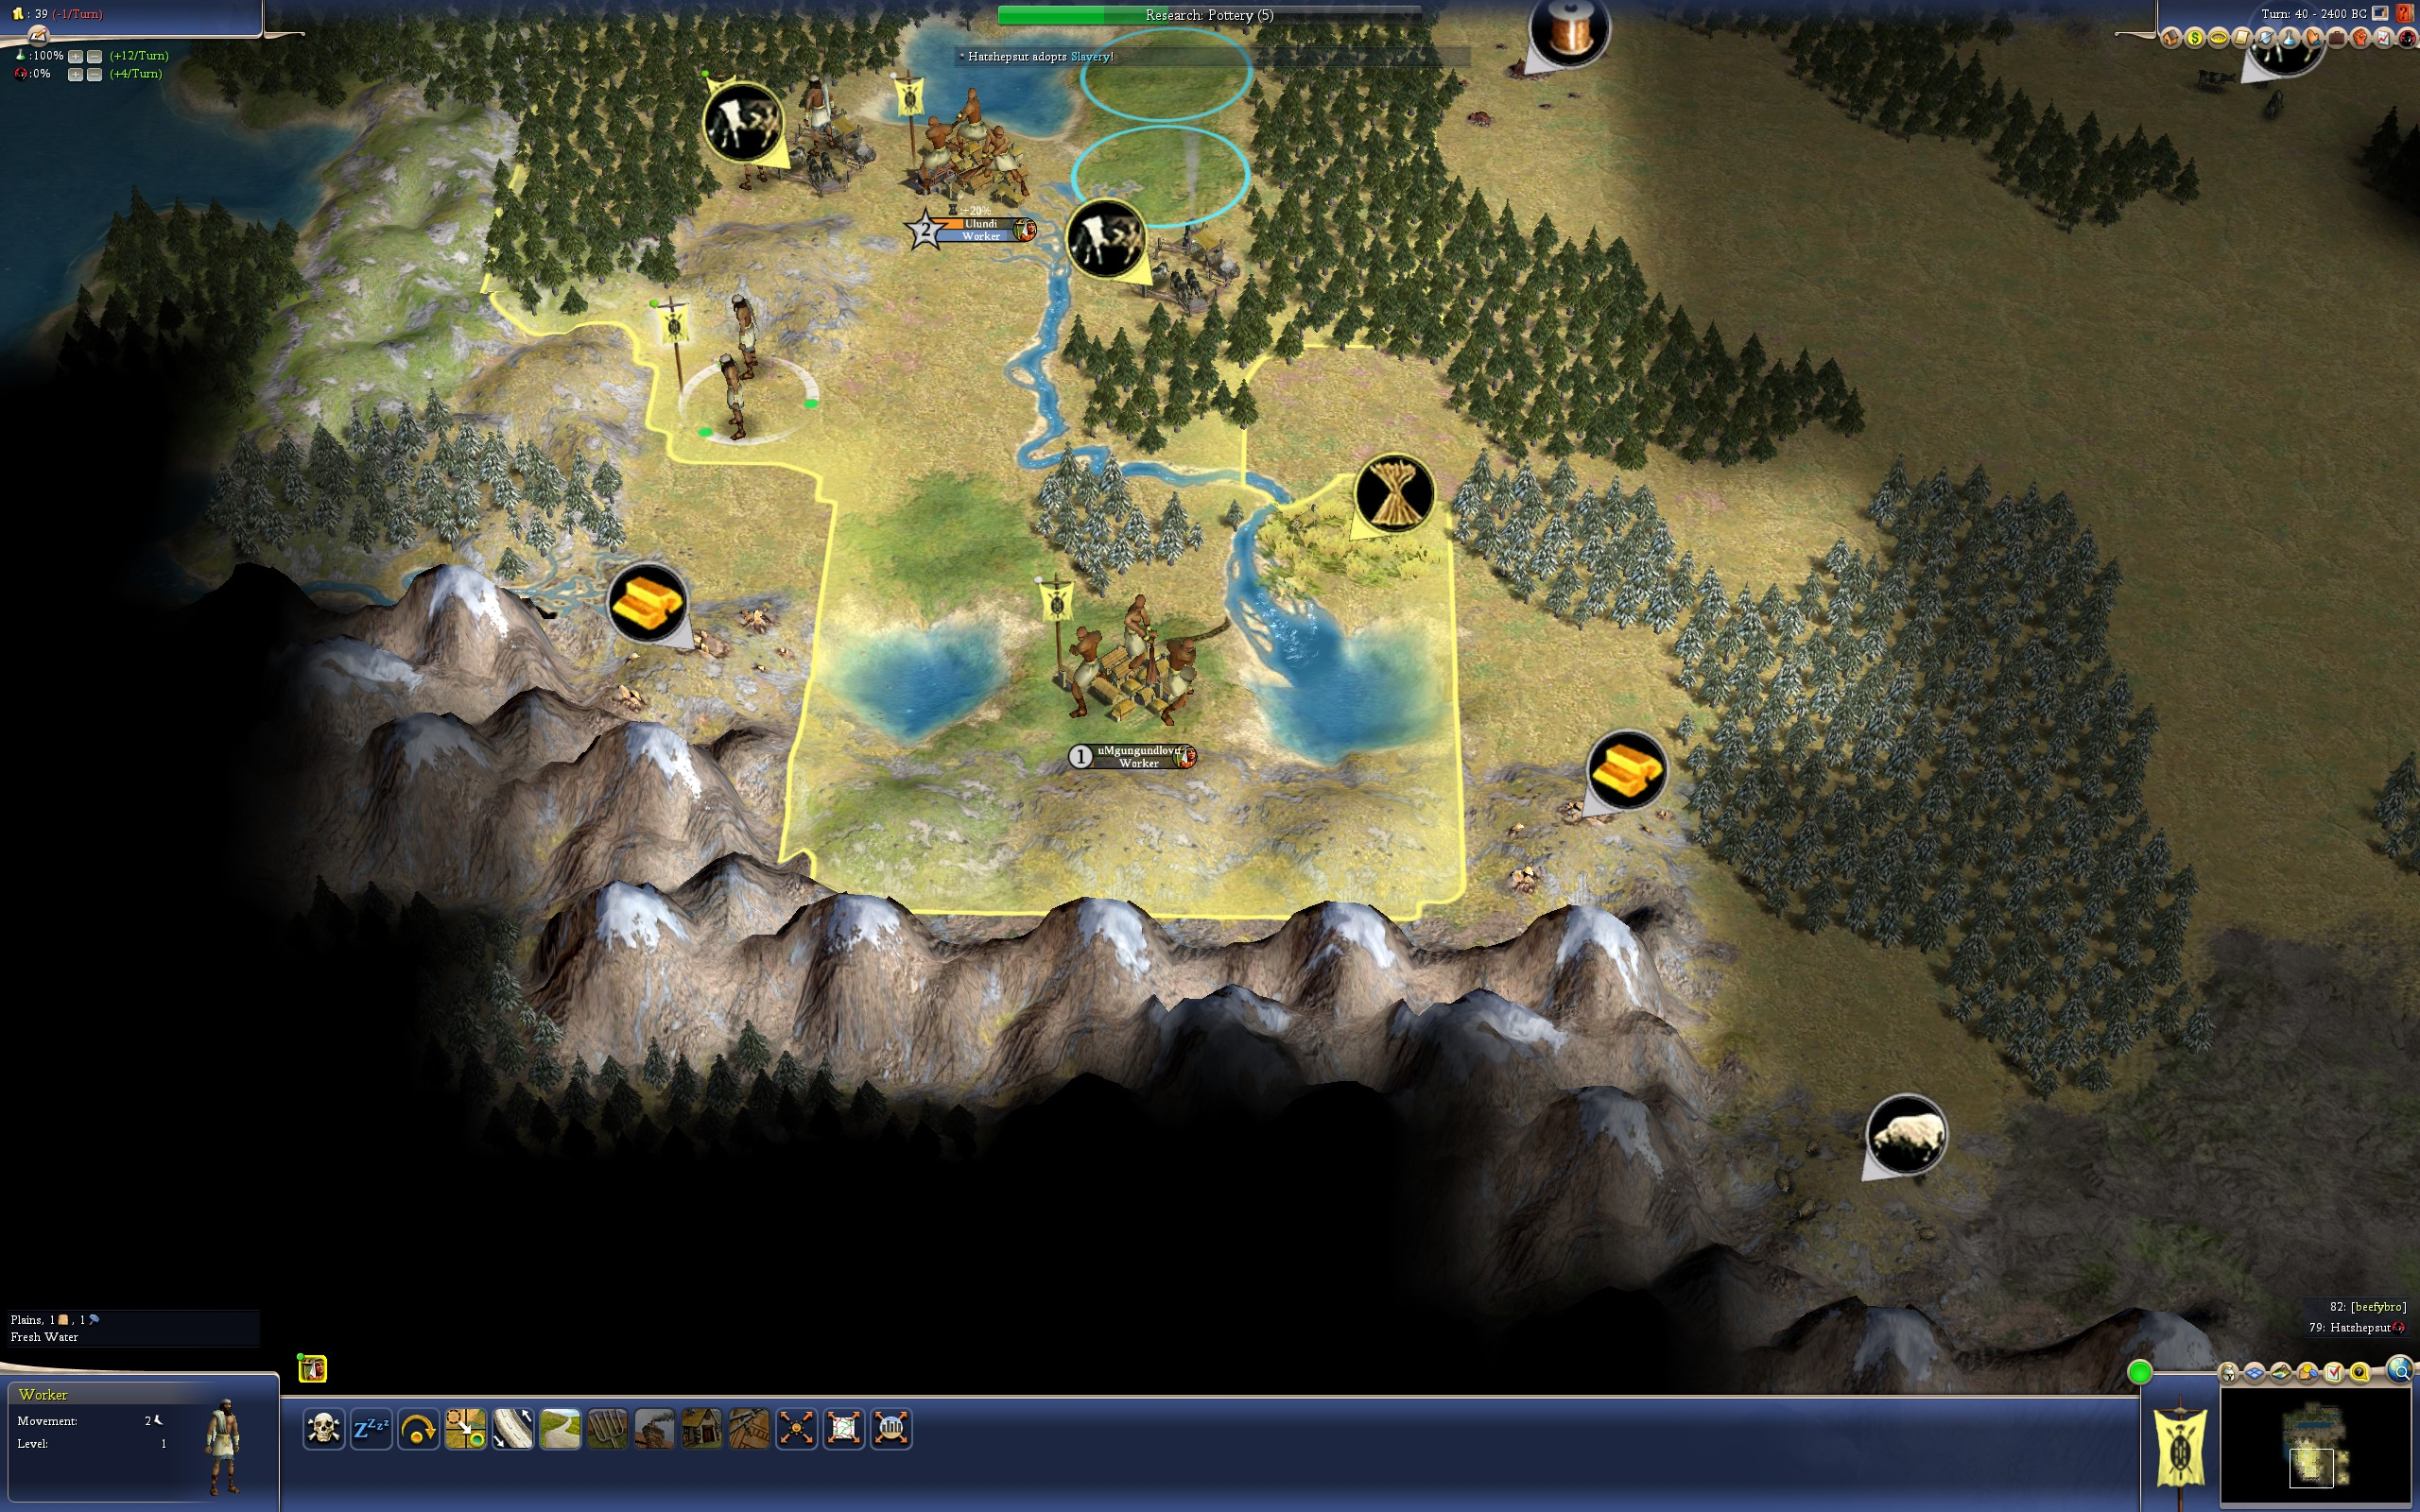
\includegraphics[width=1.0\textwidth]{13}

Gold city is placed and one of the workers from the capital is headed down to help jump-start this
excellent city. The capital is only size 2 and both cows are already improved, so the worker left behind
can be on chop duty while the second worker starts to do chops for the new city. That will help the new city
produce it's own worker and the worker that's currently there can go back to roaming to where he's most
needed.

I'm going into a fair bit of detail here explaining what I'm doing with my workers. That's intentional. Having
lots of early-game workers and using them optimally is the MOST IMPORTANT thing to get right in most openers.

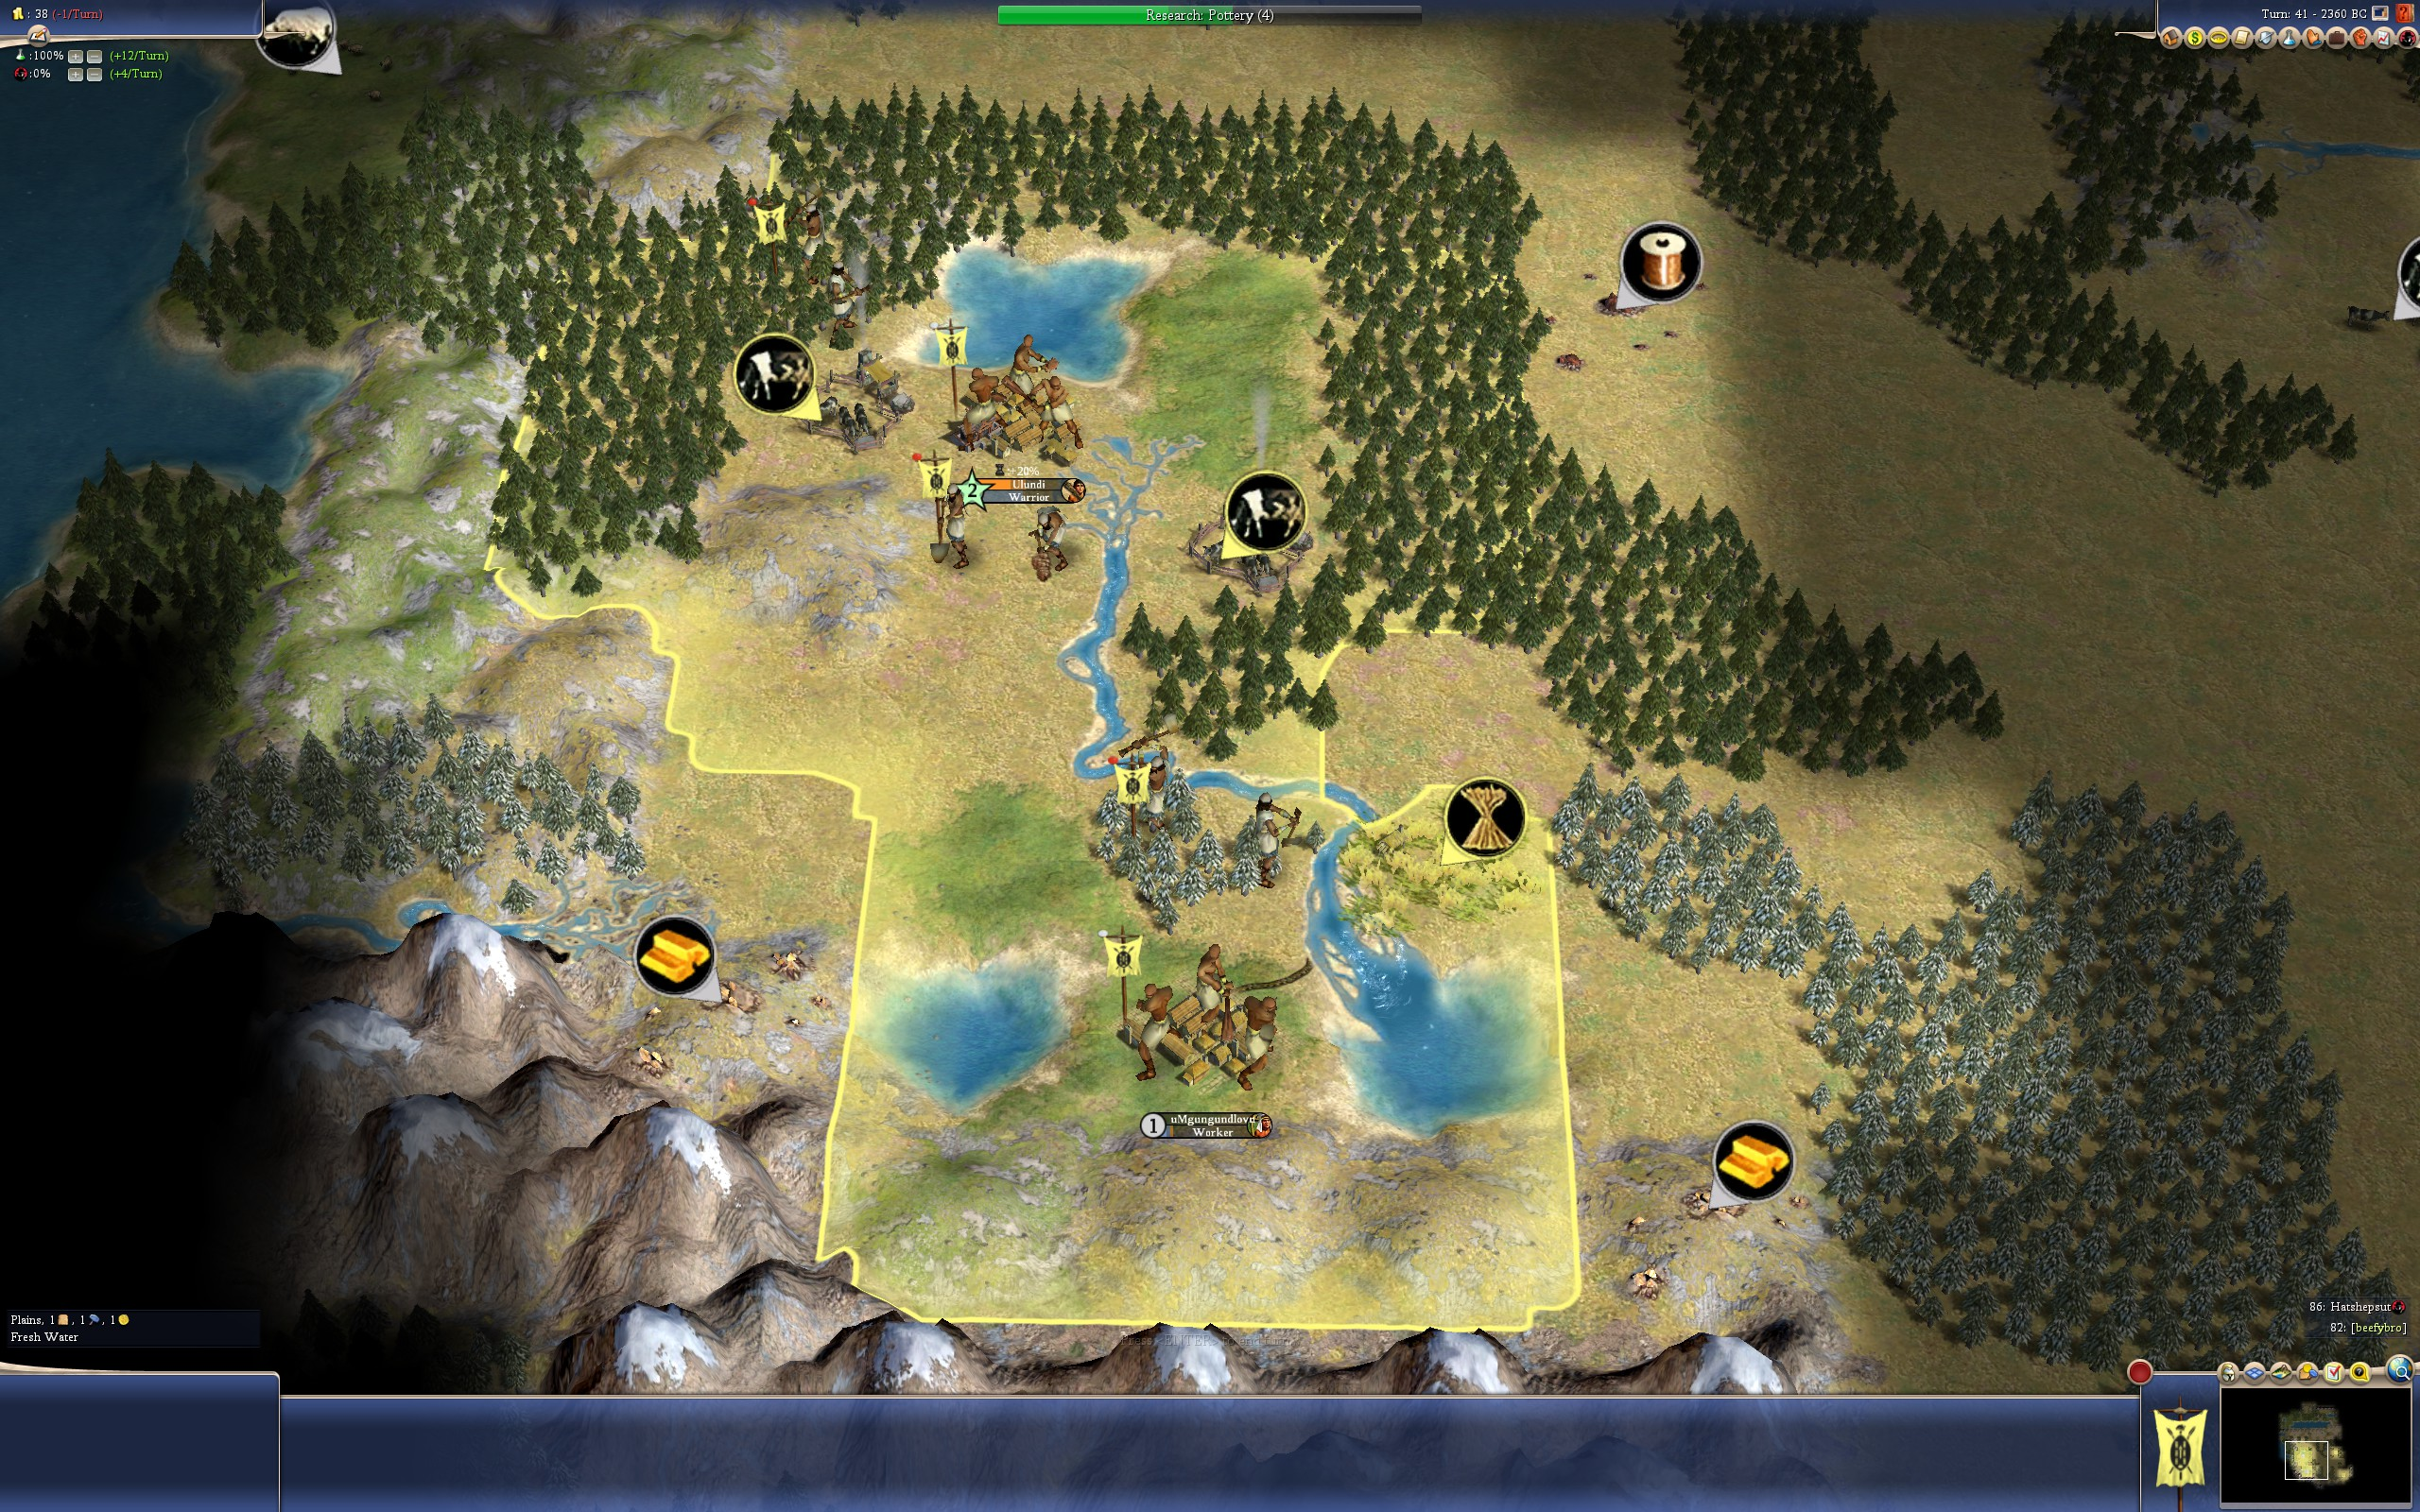
\includegraphics[width=1.0\textwidth]{14}

The capital has made yet another worker and is now working on an escort for the next settler. The new worker
is making a critical road south of the capital. This will officially connect the capital to the river and
the river connects my expansion, so this will make a +1 commerce trade route in both cities. +2 commerce
is nothing to sneeze at this early in the game.

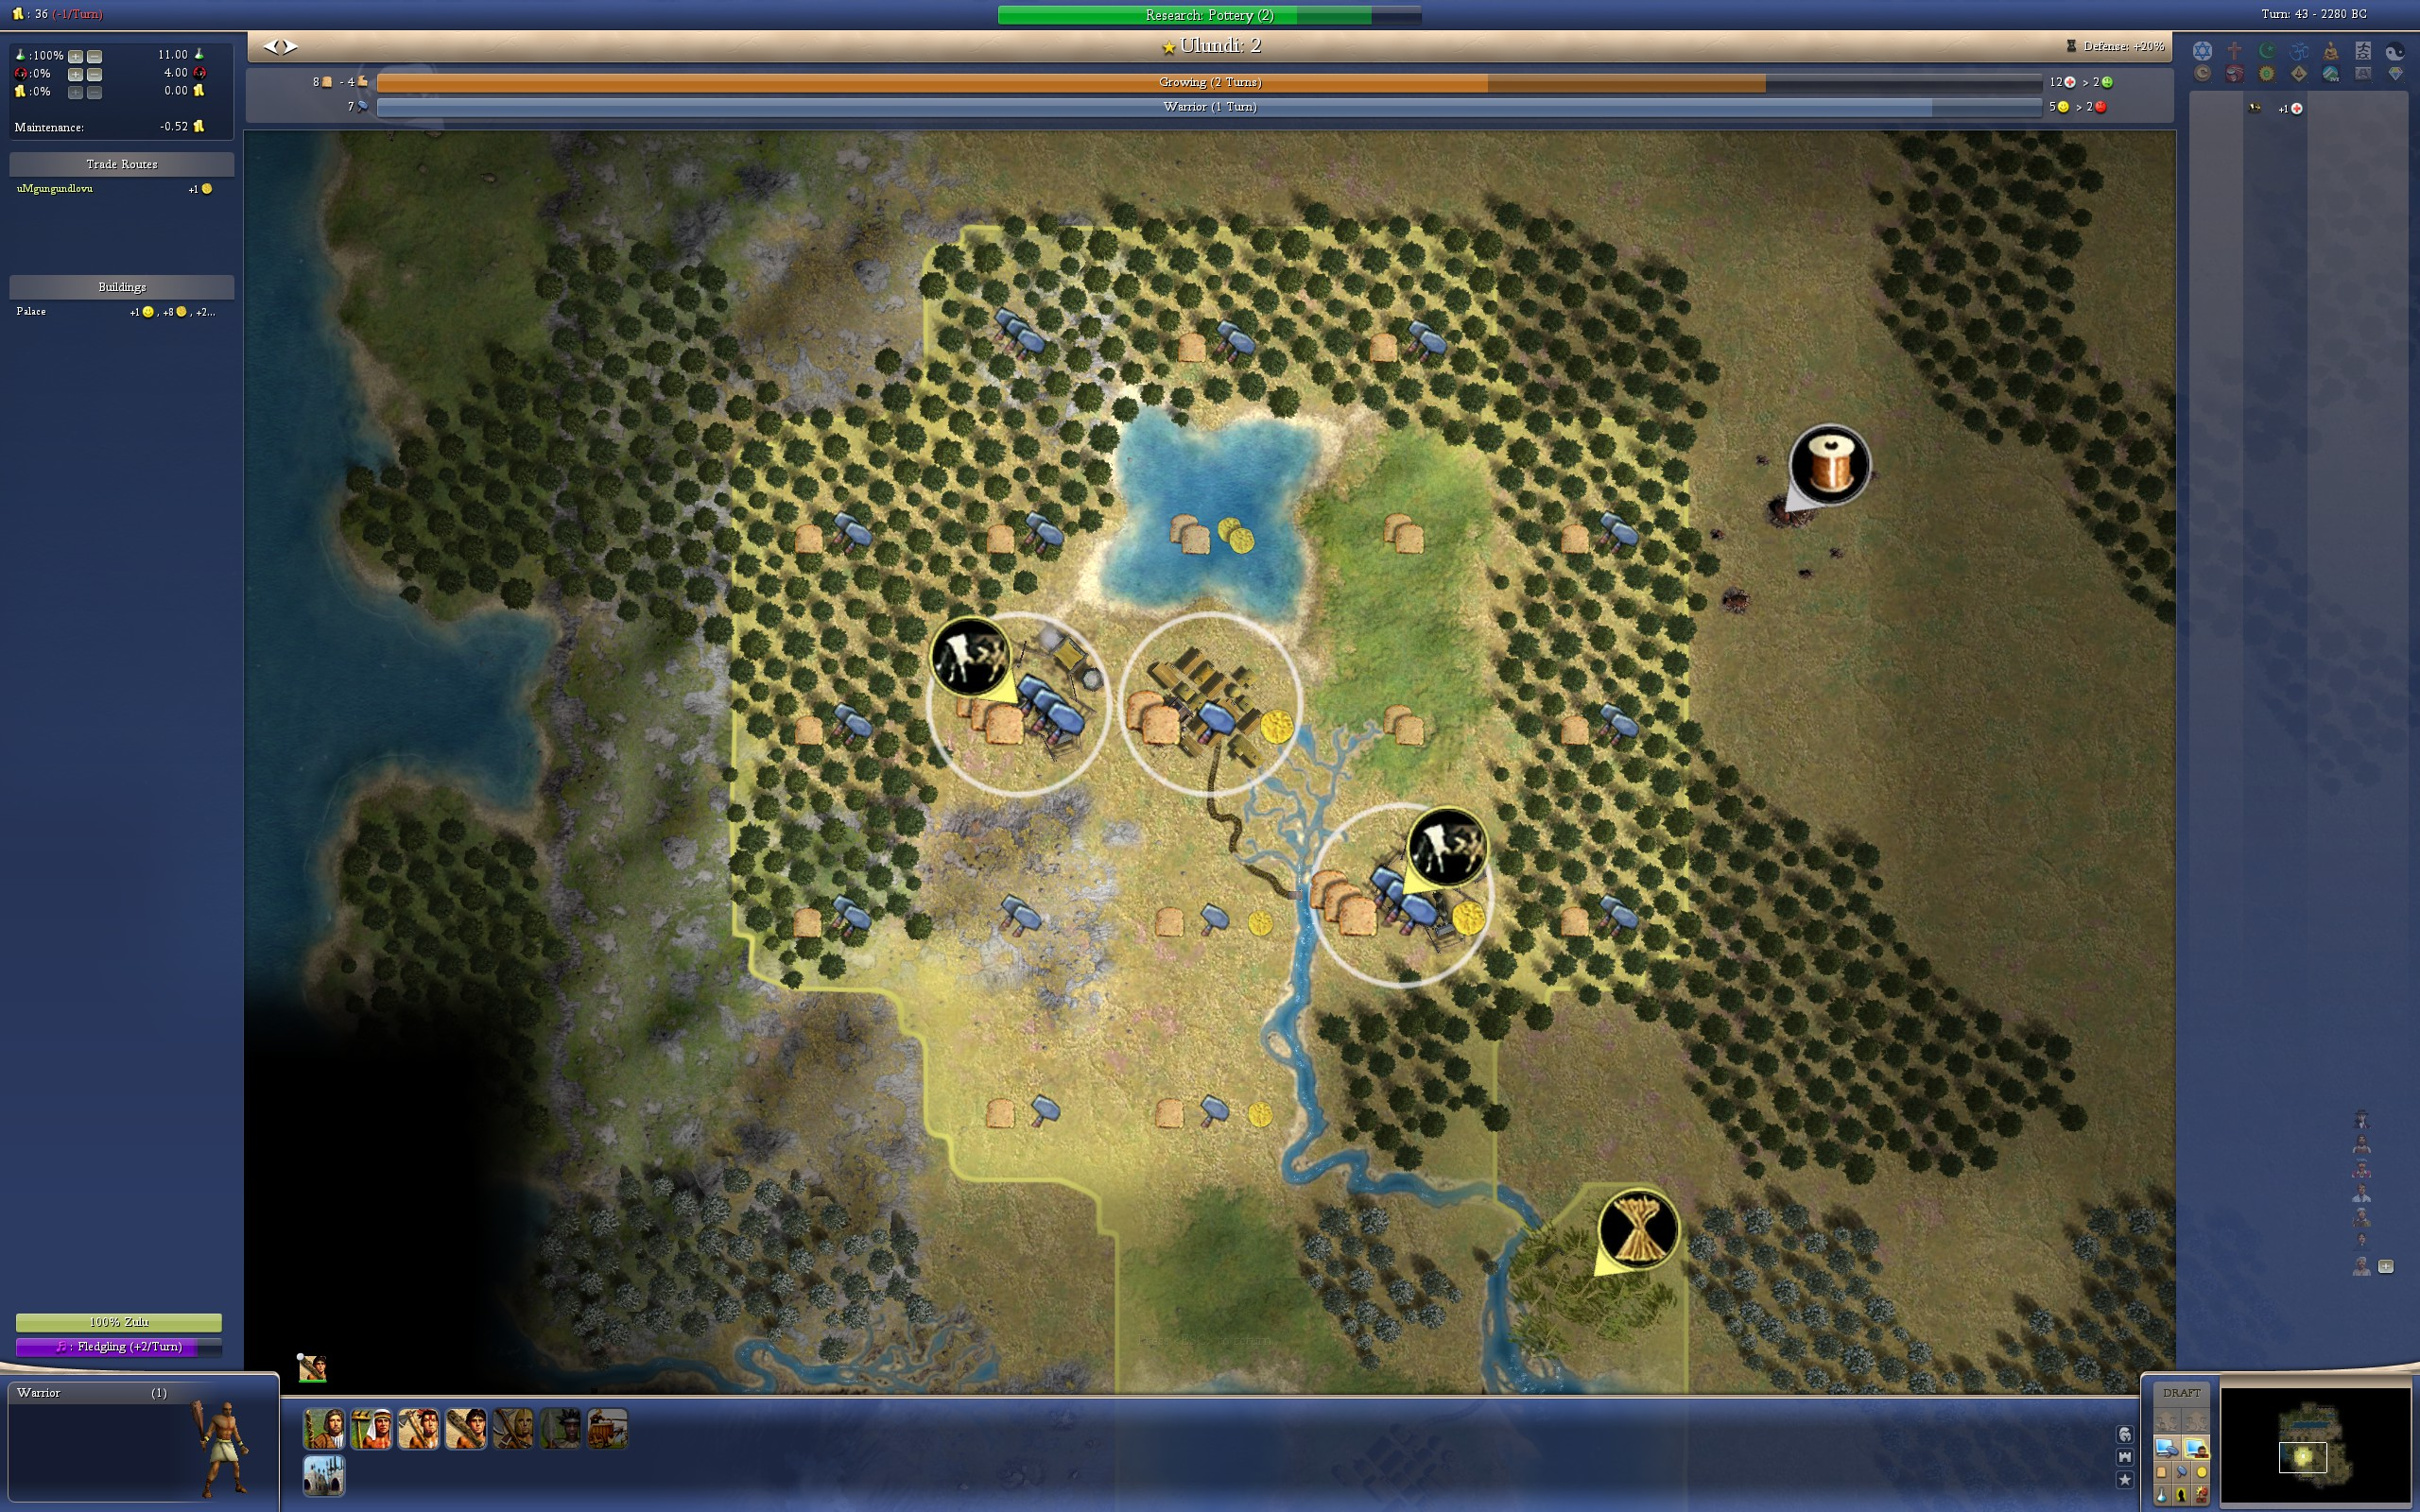
\includegraphics[width=1.0\textwidth]{15}

Here's a quick look inside my capital. The cows aren't great food sources, but the 3 hammers each are
a fanatastic early boost to my production. Having a lot of cows means your capital starts strong but
fizzles later due to lack of food. Right now, I'm putting these hammers into an all-out rex. Going for
an early wonder would be an option here too.

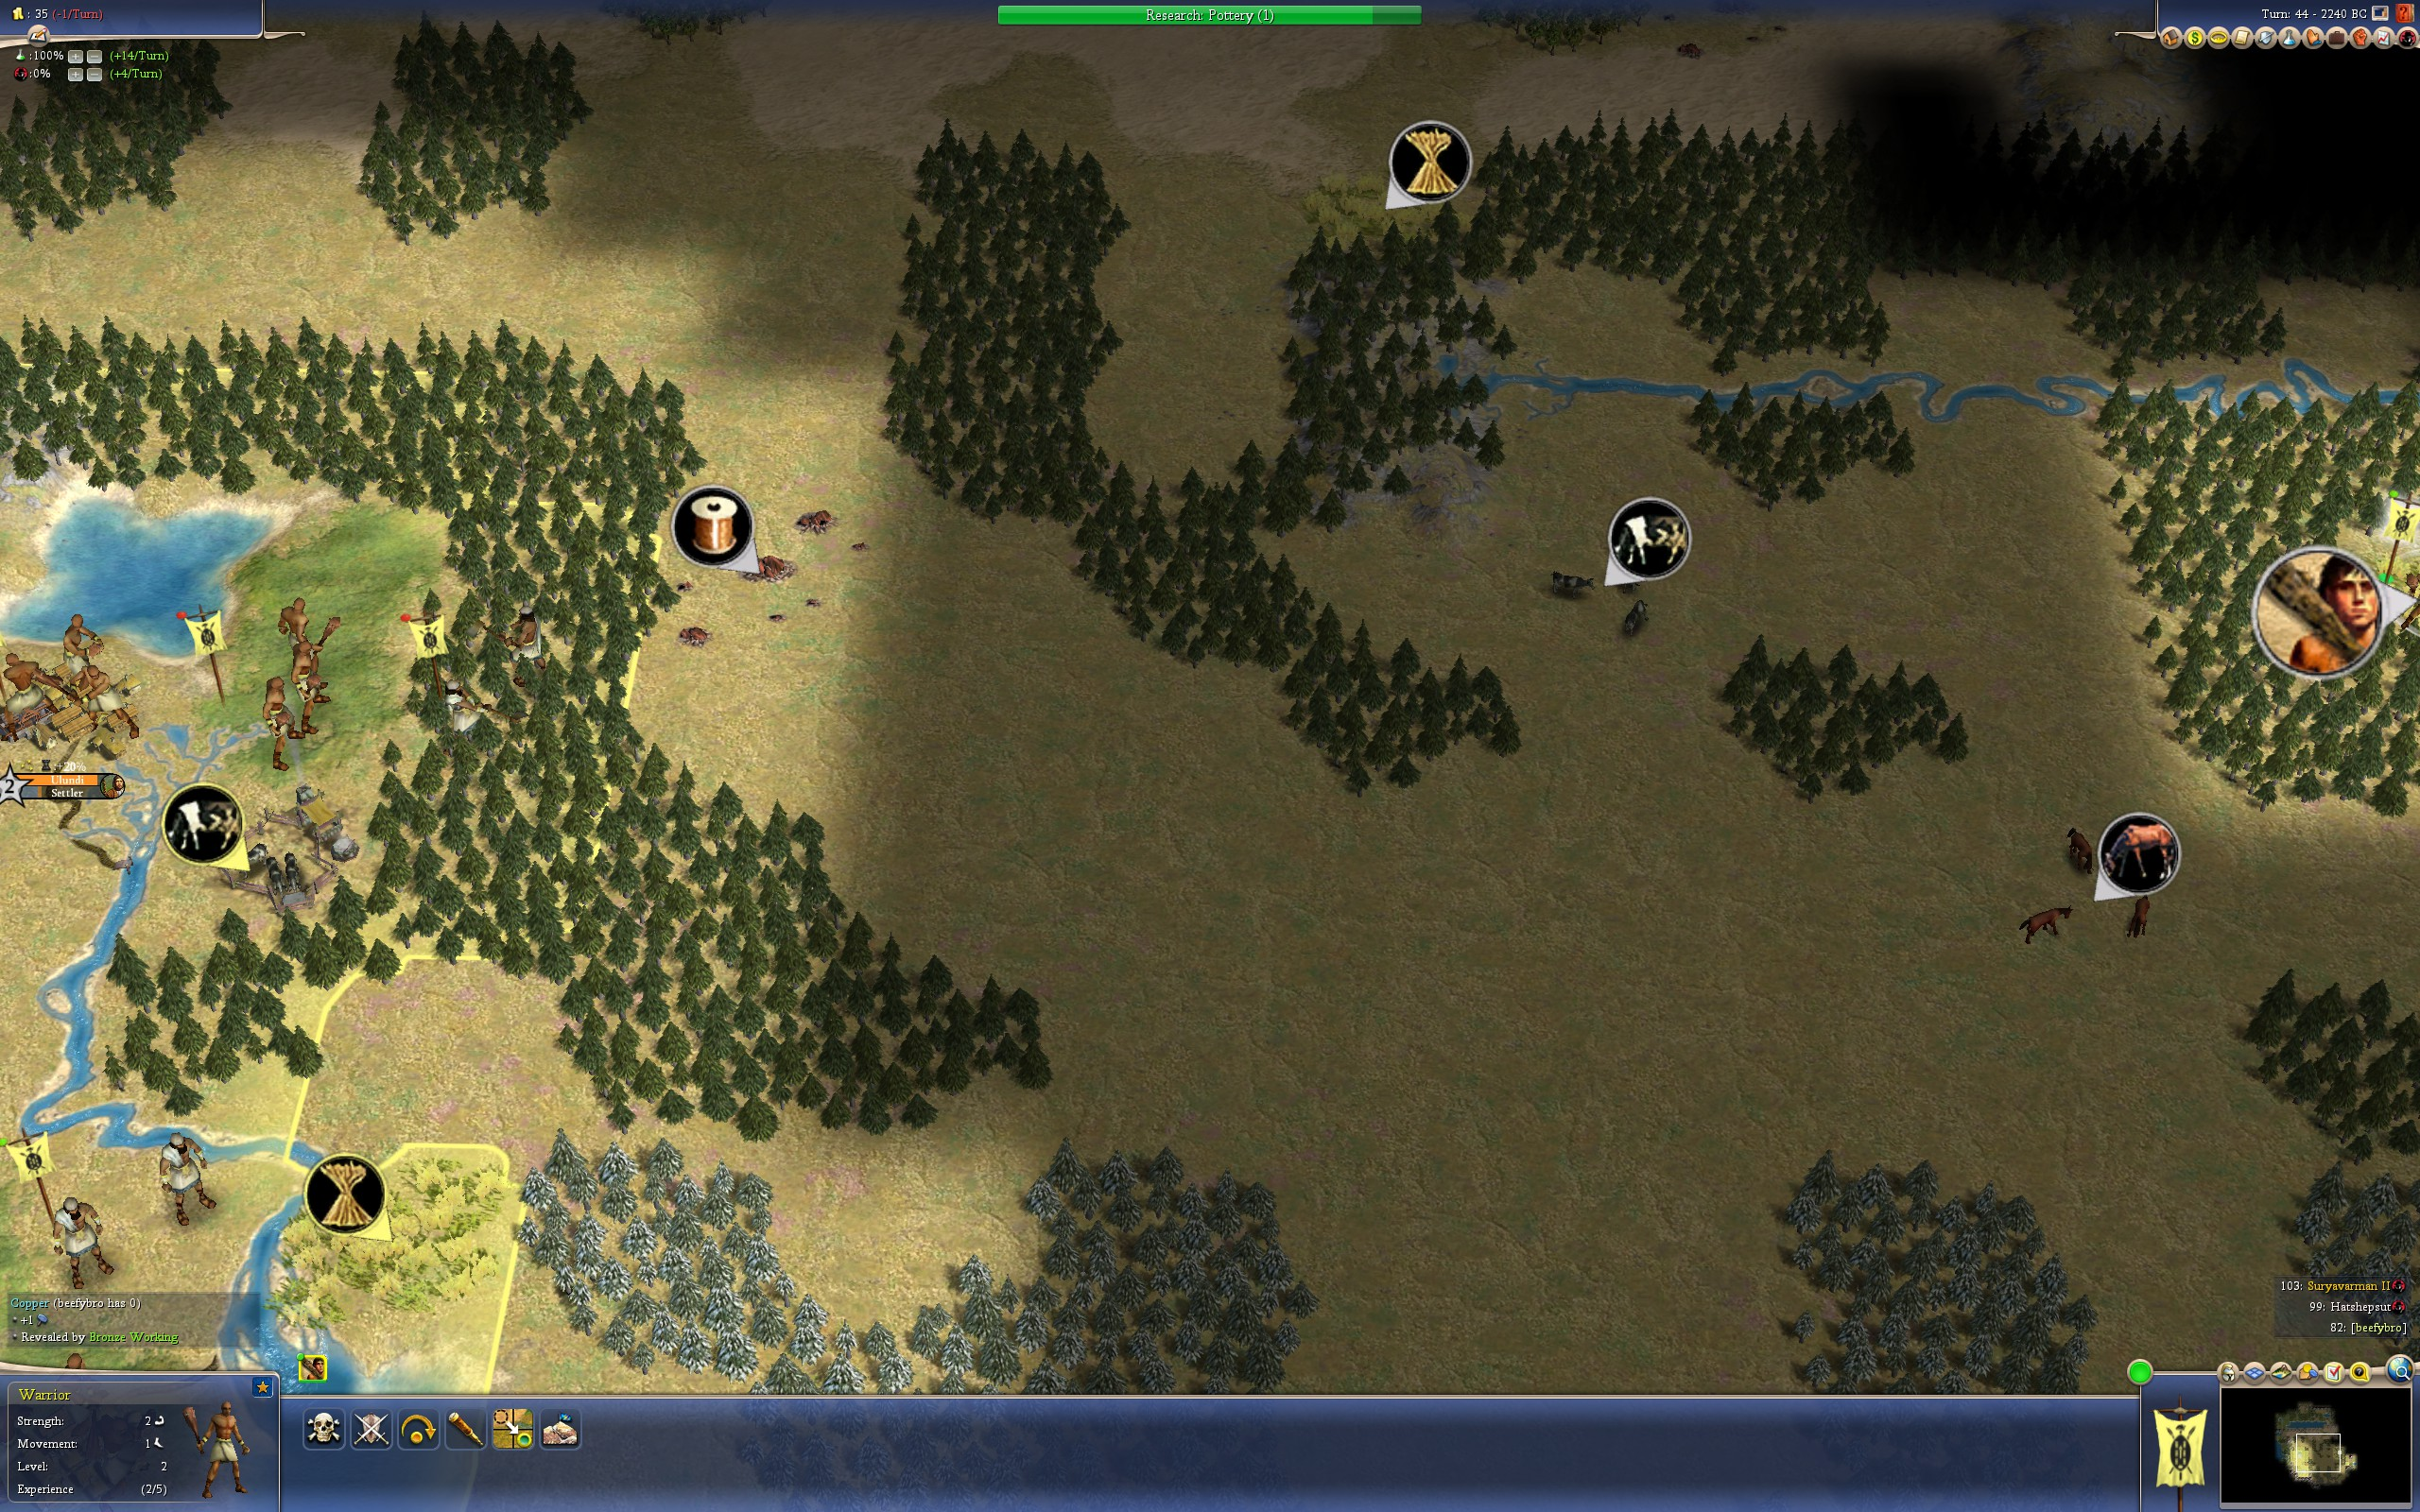
\includegraphics[width=1.0\textwidth]{16}

A quick look to my east where I plan to settle next. Picking up bronze is top priority and grabbing the
river futher to the east is next after that.

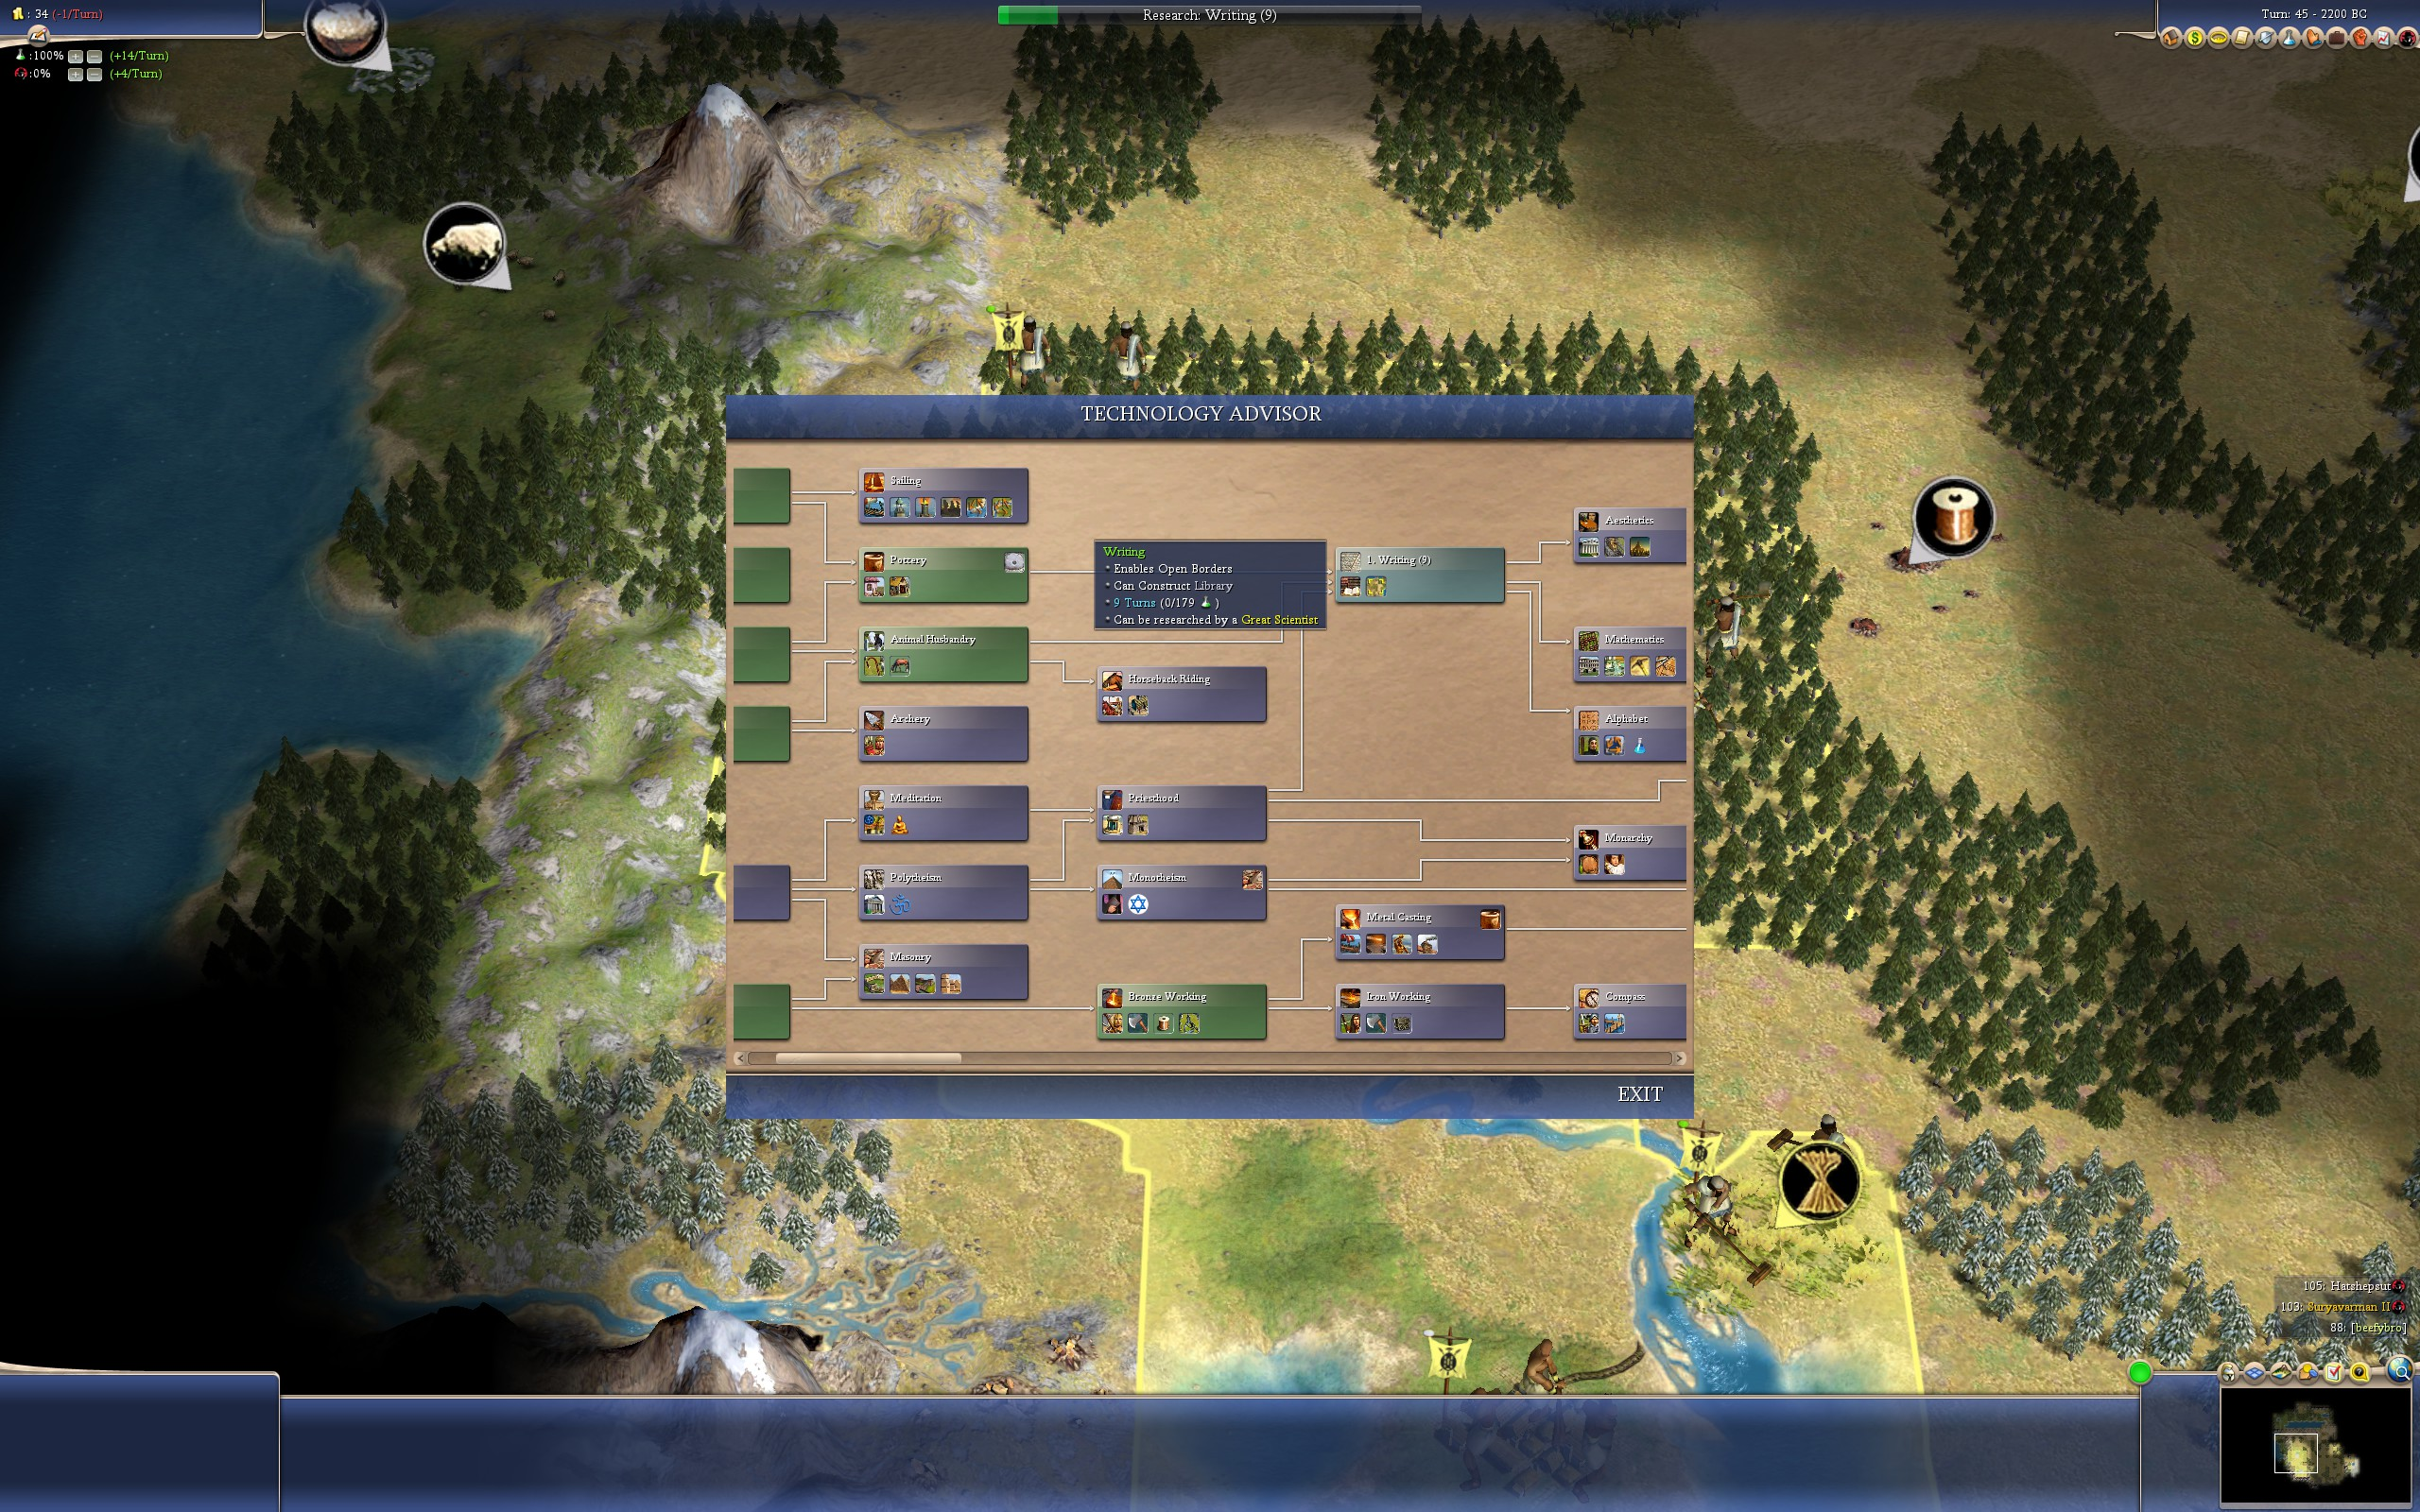
\includegraphics[width=1.0\textwidth]{17}

Pottery is done. If I were industrial or had stone or marble nearby, I'd definitely be considering a wonder
here, but that's not the situation here so I go for Writing next which is standard play. Writing unlocks
OB and libraries, neither of which I'll be using for a while. AIs love getting religions; if this were a human
game, you might consider going for one here. The right play here was probably going mysticism in order to unlock
monuments so that my gold city could have gotten a faster border pop (both golds were in the outer BFC).

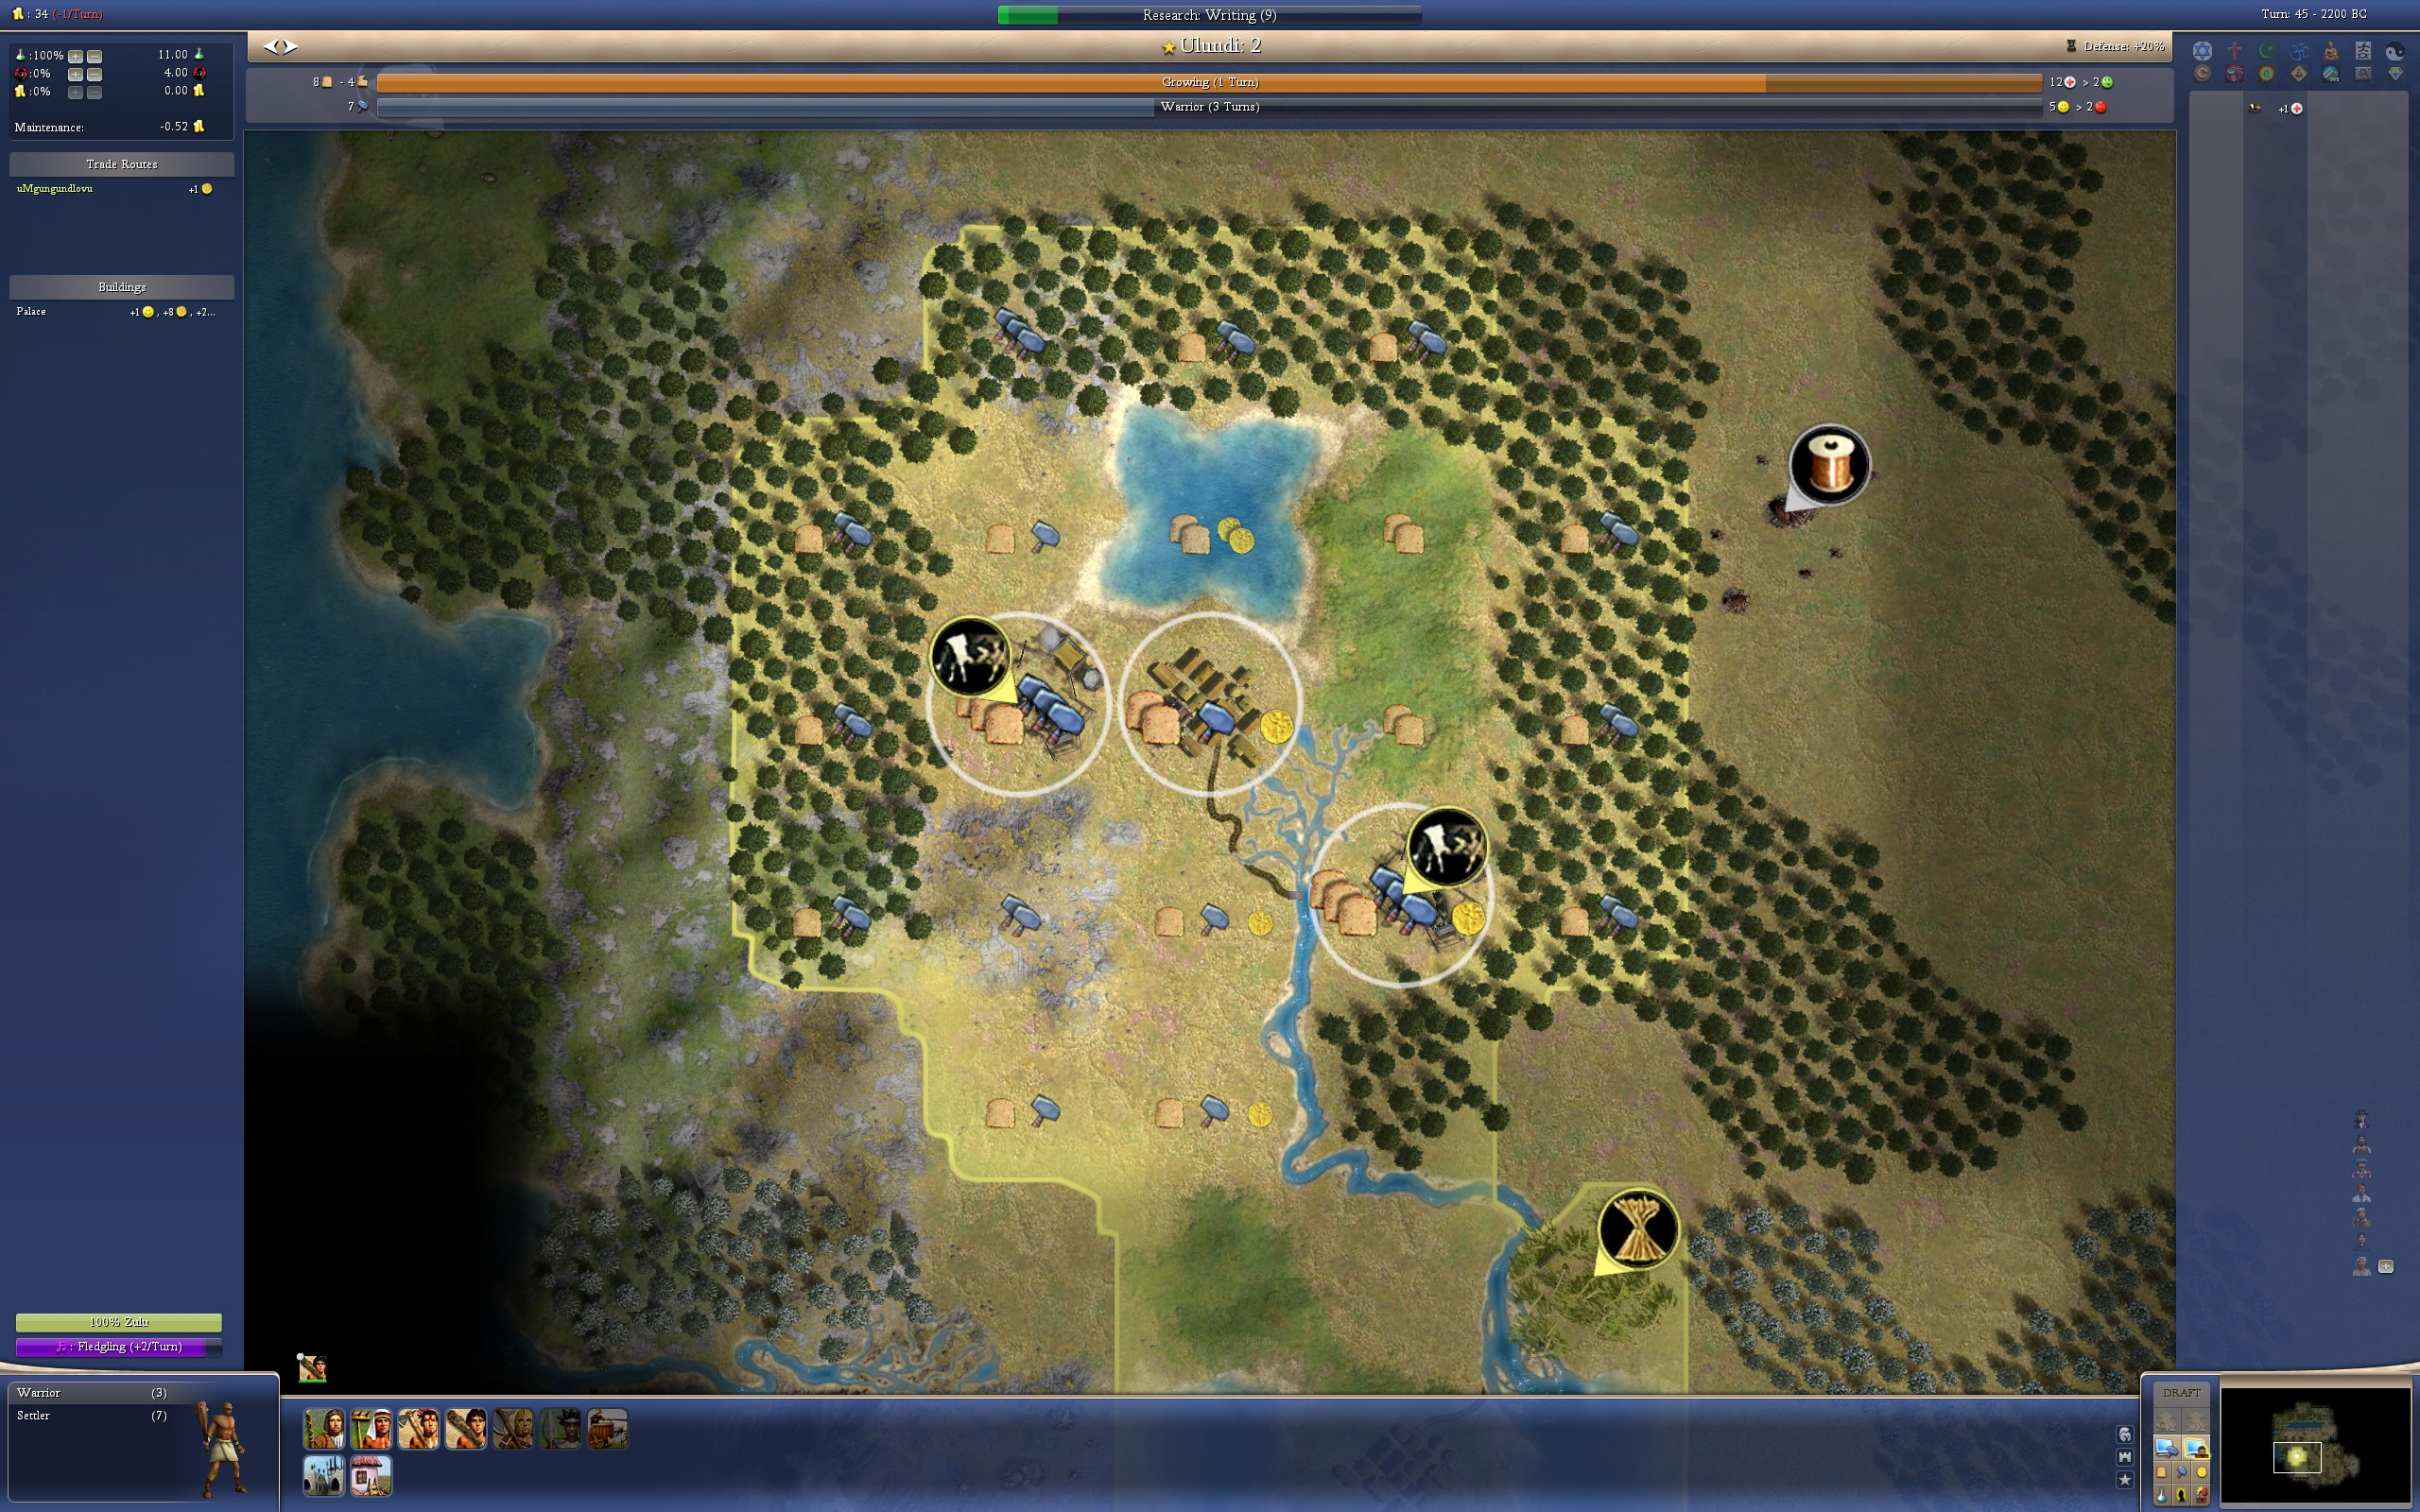
\includegraphics[width=1.0\textwidth]{18}

This shot is to show the trade route connection to my gold city. It also shows a common technique of
swapping production between items that block city growth (settler, worker) and non-blocking items (in
this case, a warrior). The idea here is to work the non-blocking item except when a nearby chop completes,
you swap over to the blocking item. The goal is a situation where you build blocking items almost as fast
as if you were not swapping but you also get city growth.

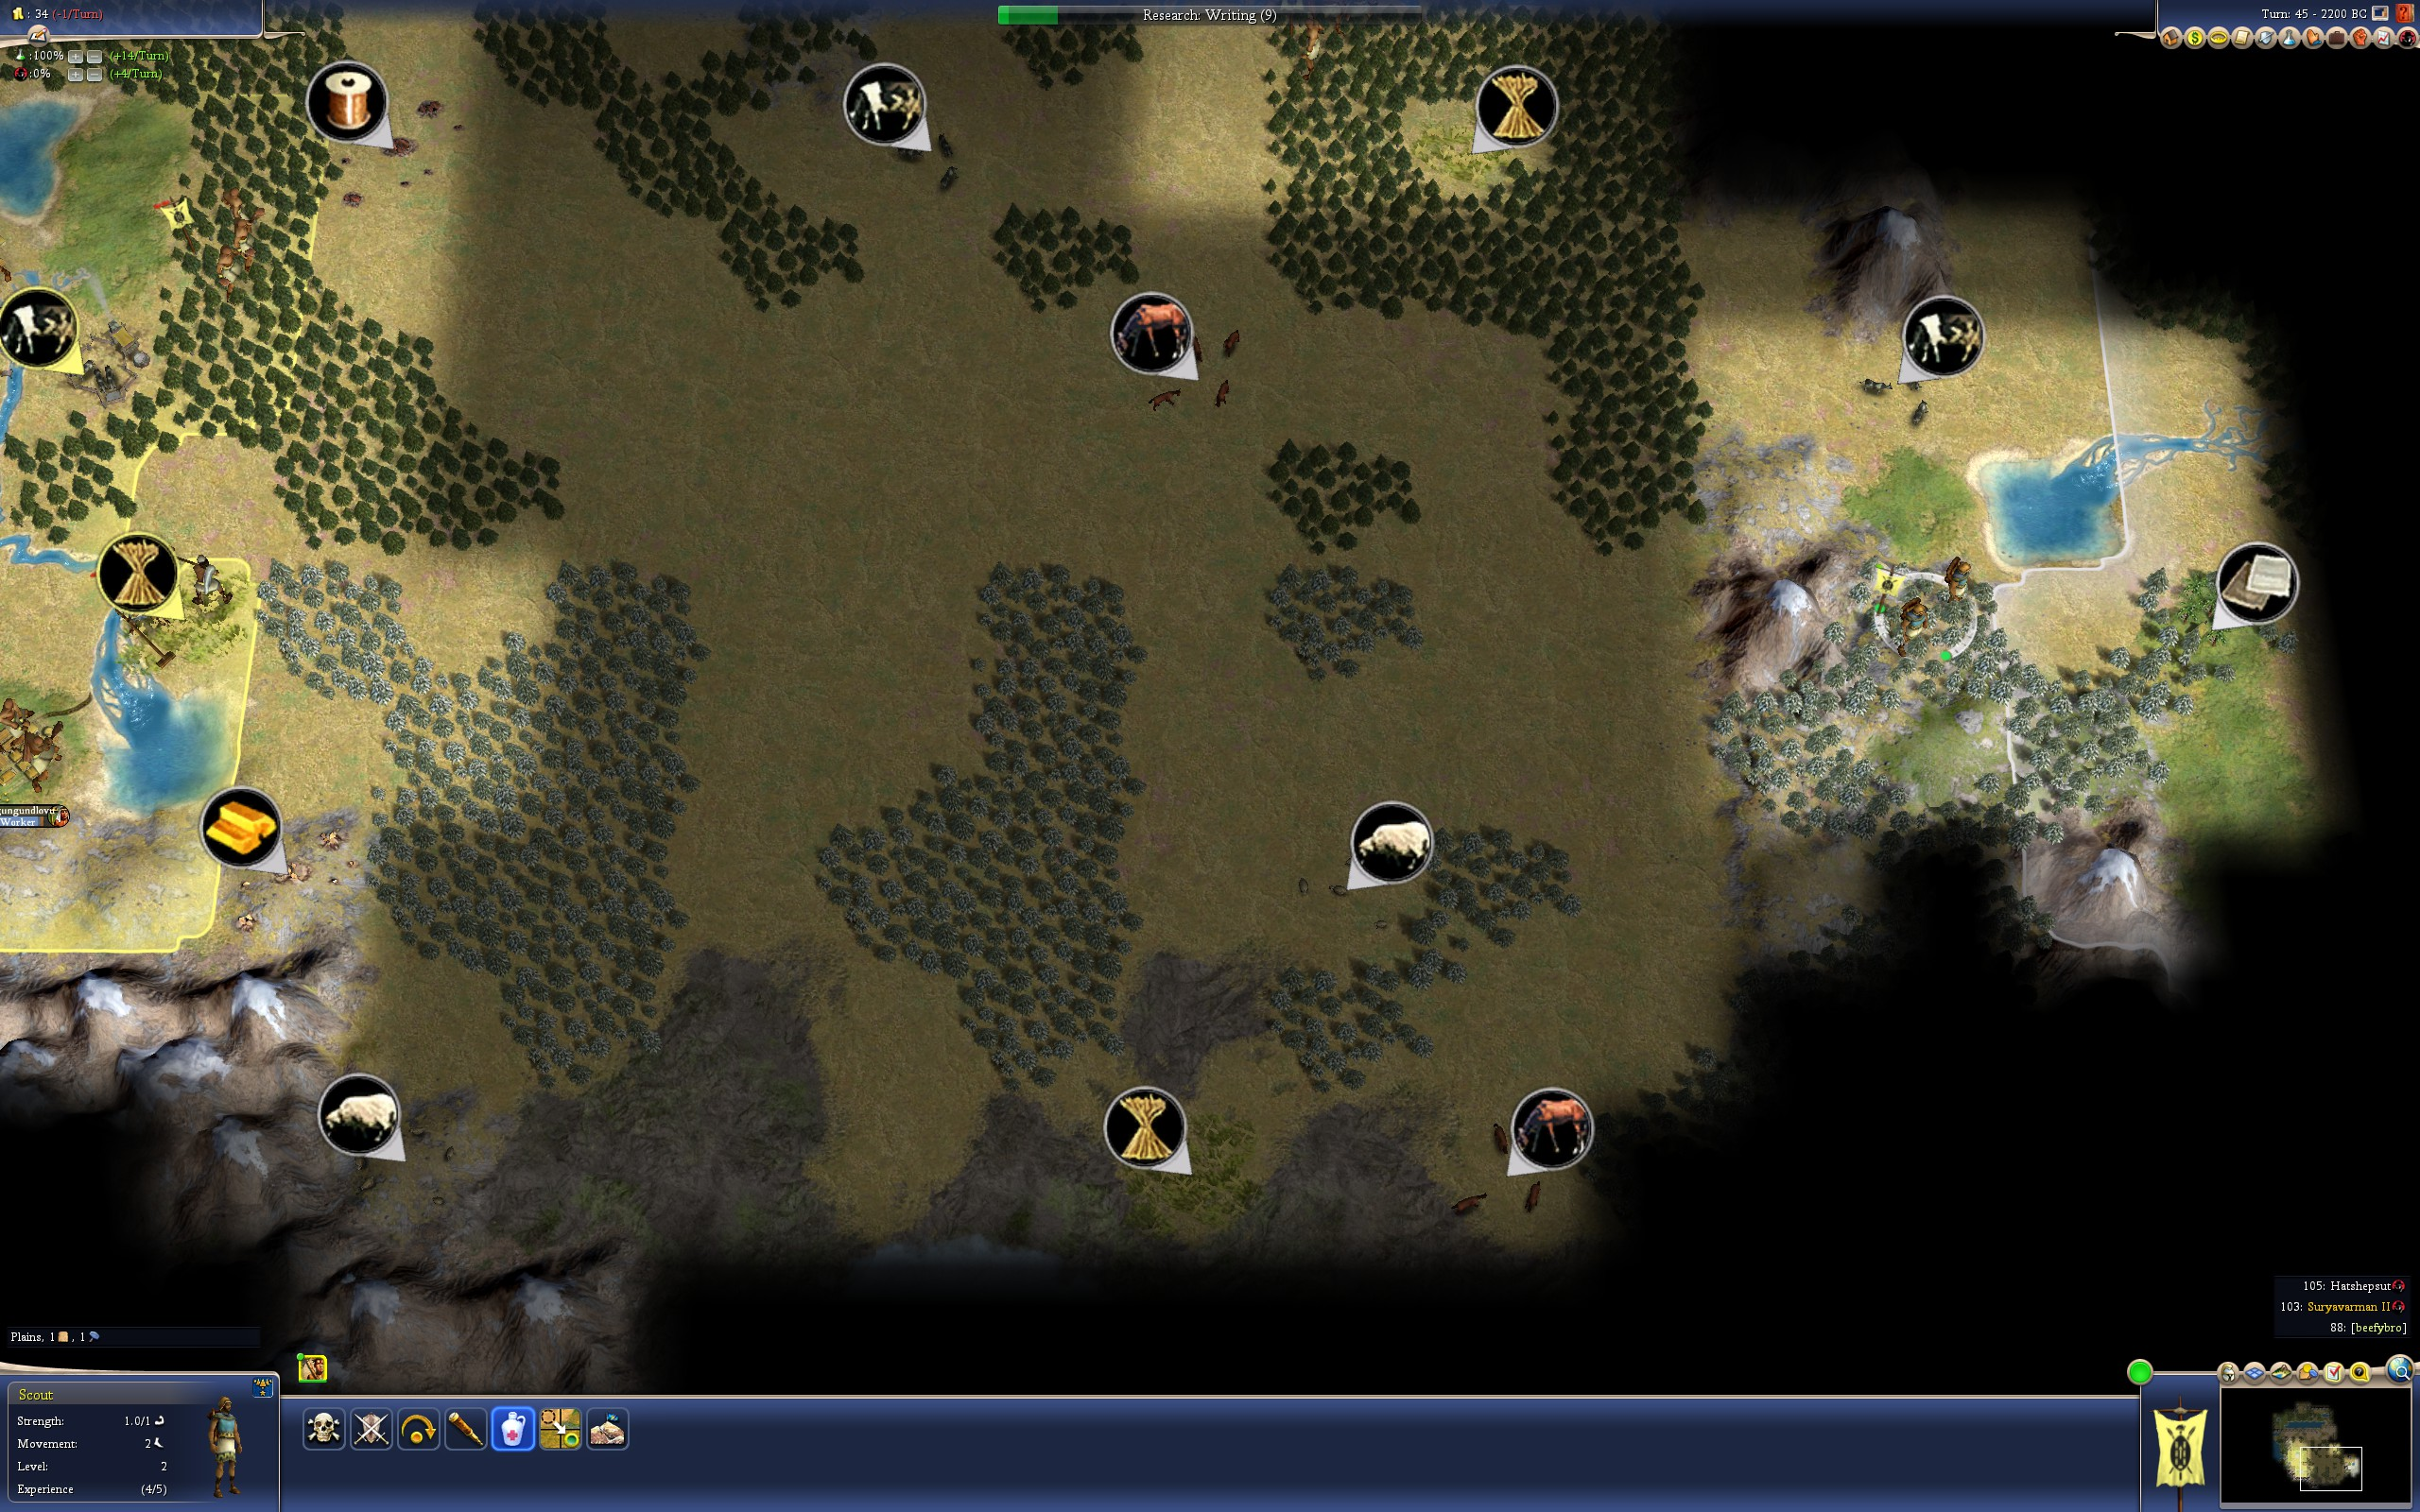
\includegraphics[width=1.0\textwidth]{19}

I've found my closest neighbor to the east, Hatshepsut (Hatty) of England. This definitely means the land
between us is in contention and I need to try to grab more of it than she does. This concept of expanding
in the direction of your closest neighbor is geopolitics 101. You grab contested land first, and then
grab guaranteed land later. Against humans, some discretion is needed as super aggresive city plants
can start wars.

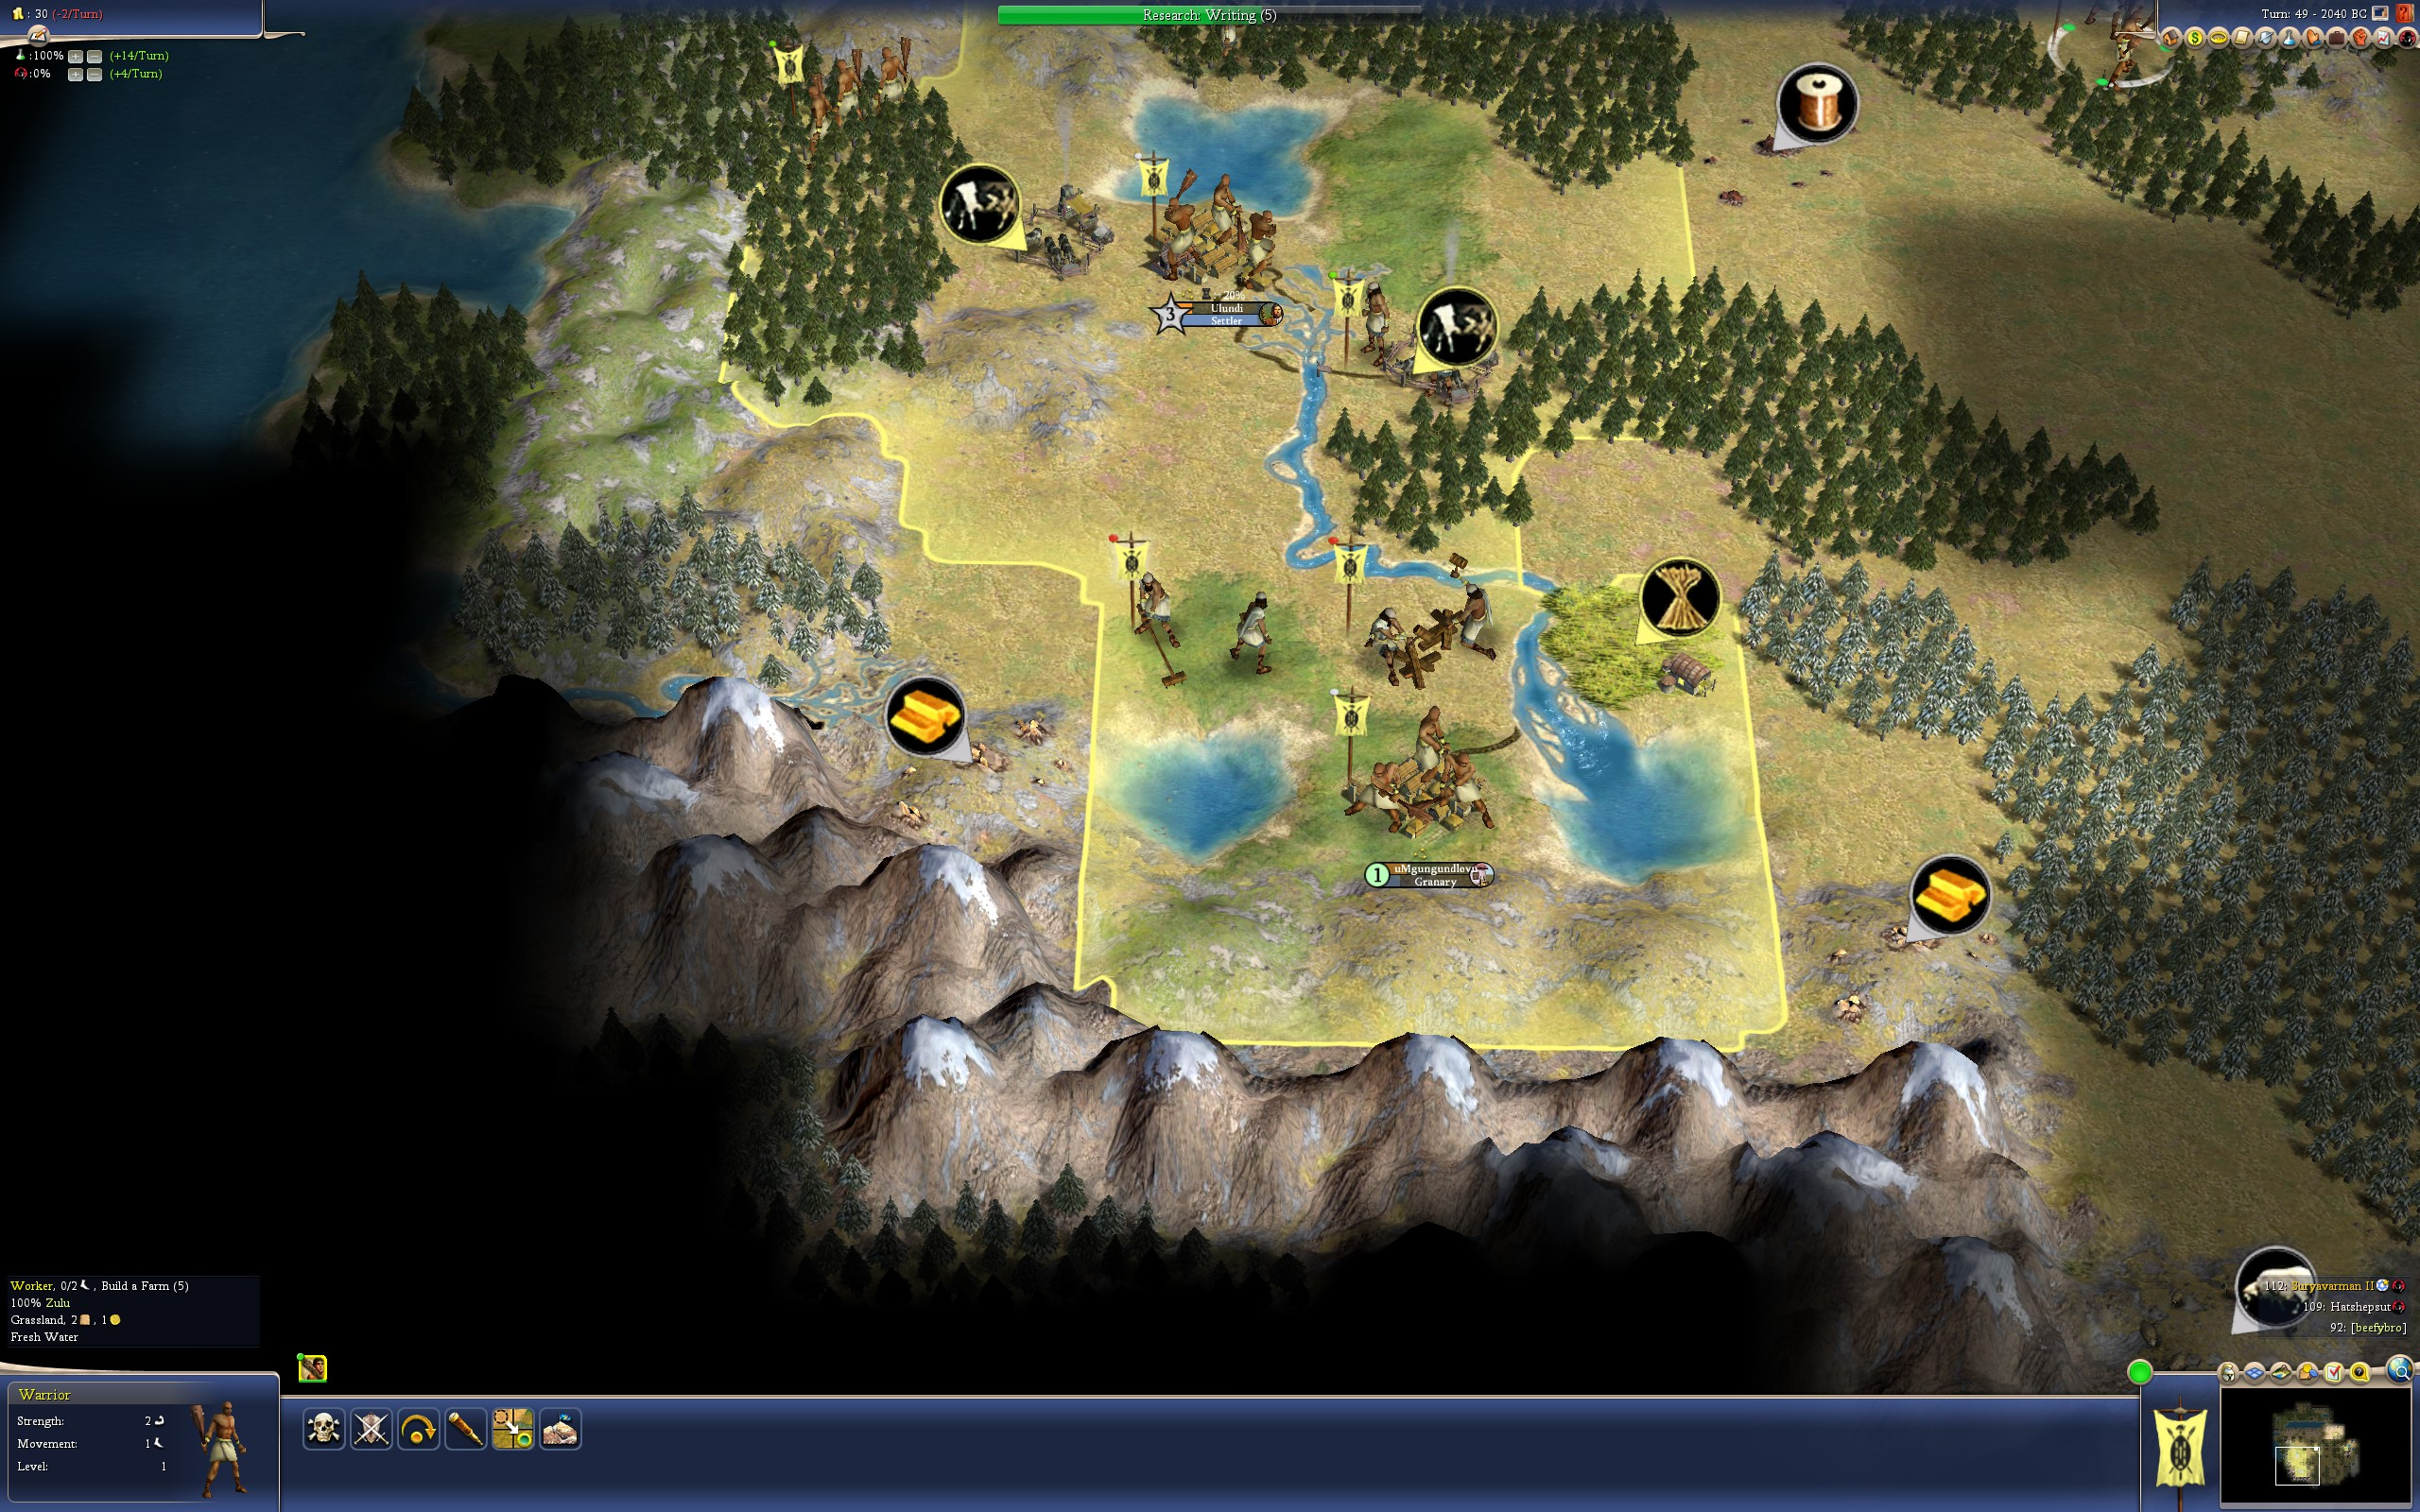
\includegraphics[width=1.0\textwidth]{21}

Only notewothy thing here is choice of tile improvements in gold city. Early-game, the only choice
for a flatland tile is cottage or farm. One of my concerns is gold city's lack of food. The wheat will
feed both gold miners, but not much more than that, so I've elected to take one of my precious green
tiles and make it a farm in order to generate a little more food surplus. I am not a fan of farming
plains tiles because it doesn't make a surplus (just even until biology) and it doesn't provide much
yield other than the food (1 hammer). Unforunately, this city won't be able to work the majority of its
tiles until biology, but it's still a great city because of the two golds.

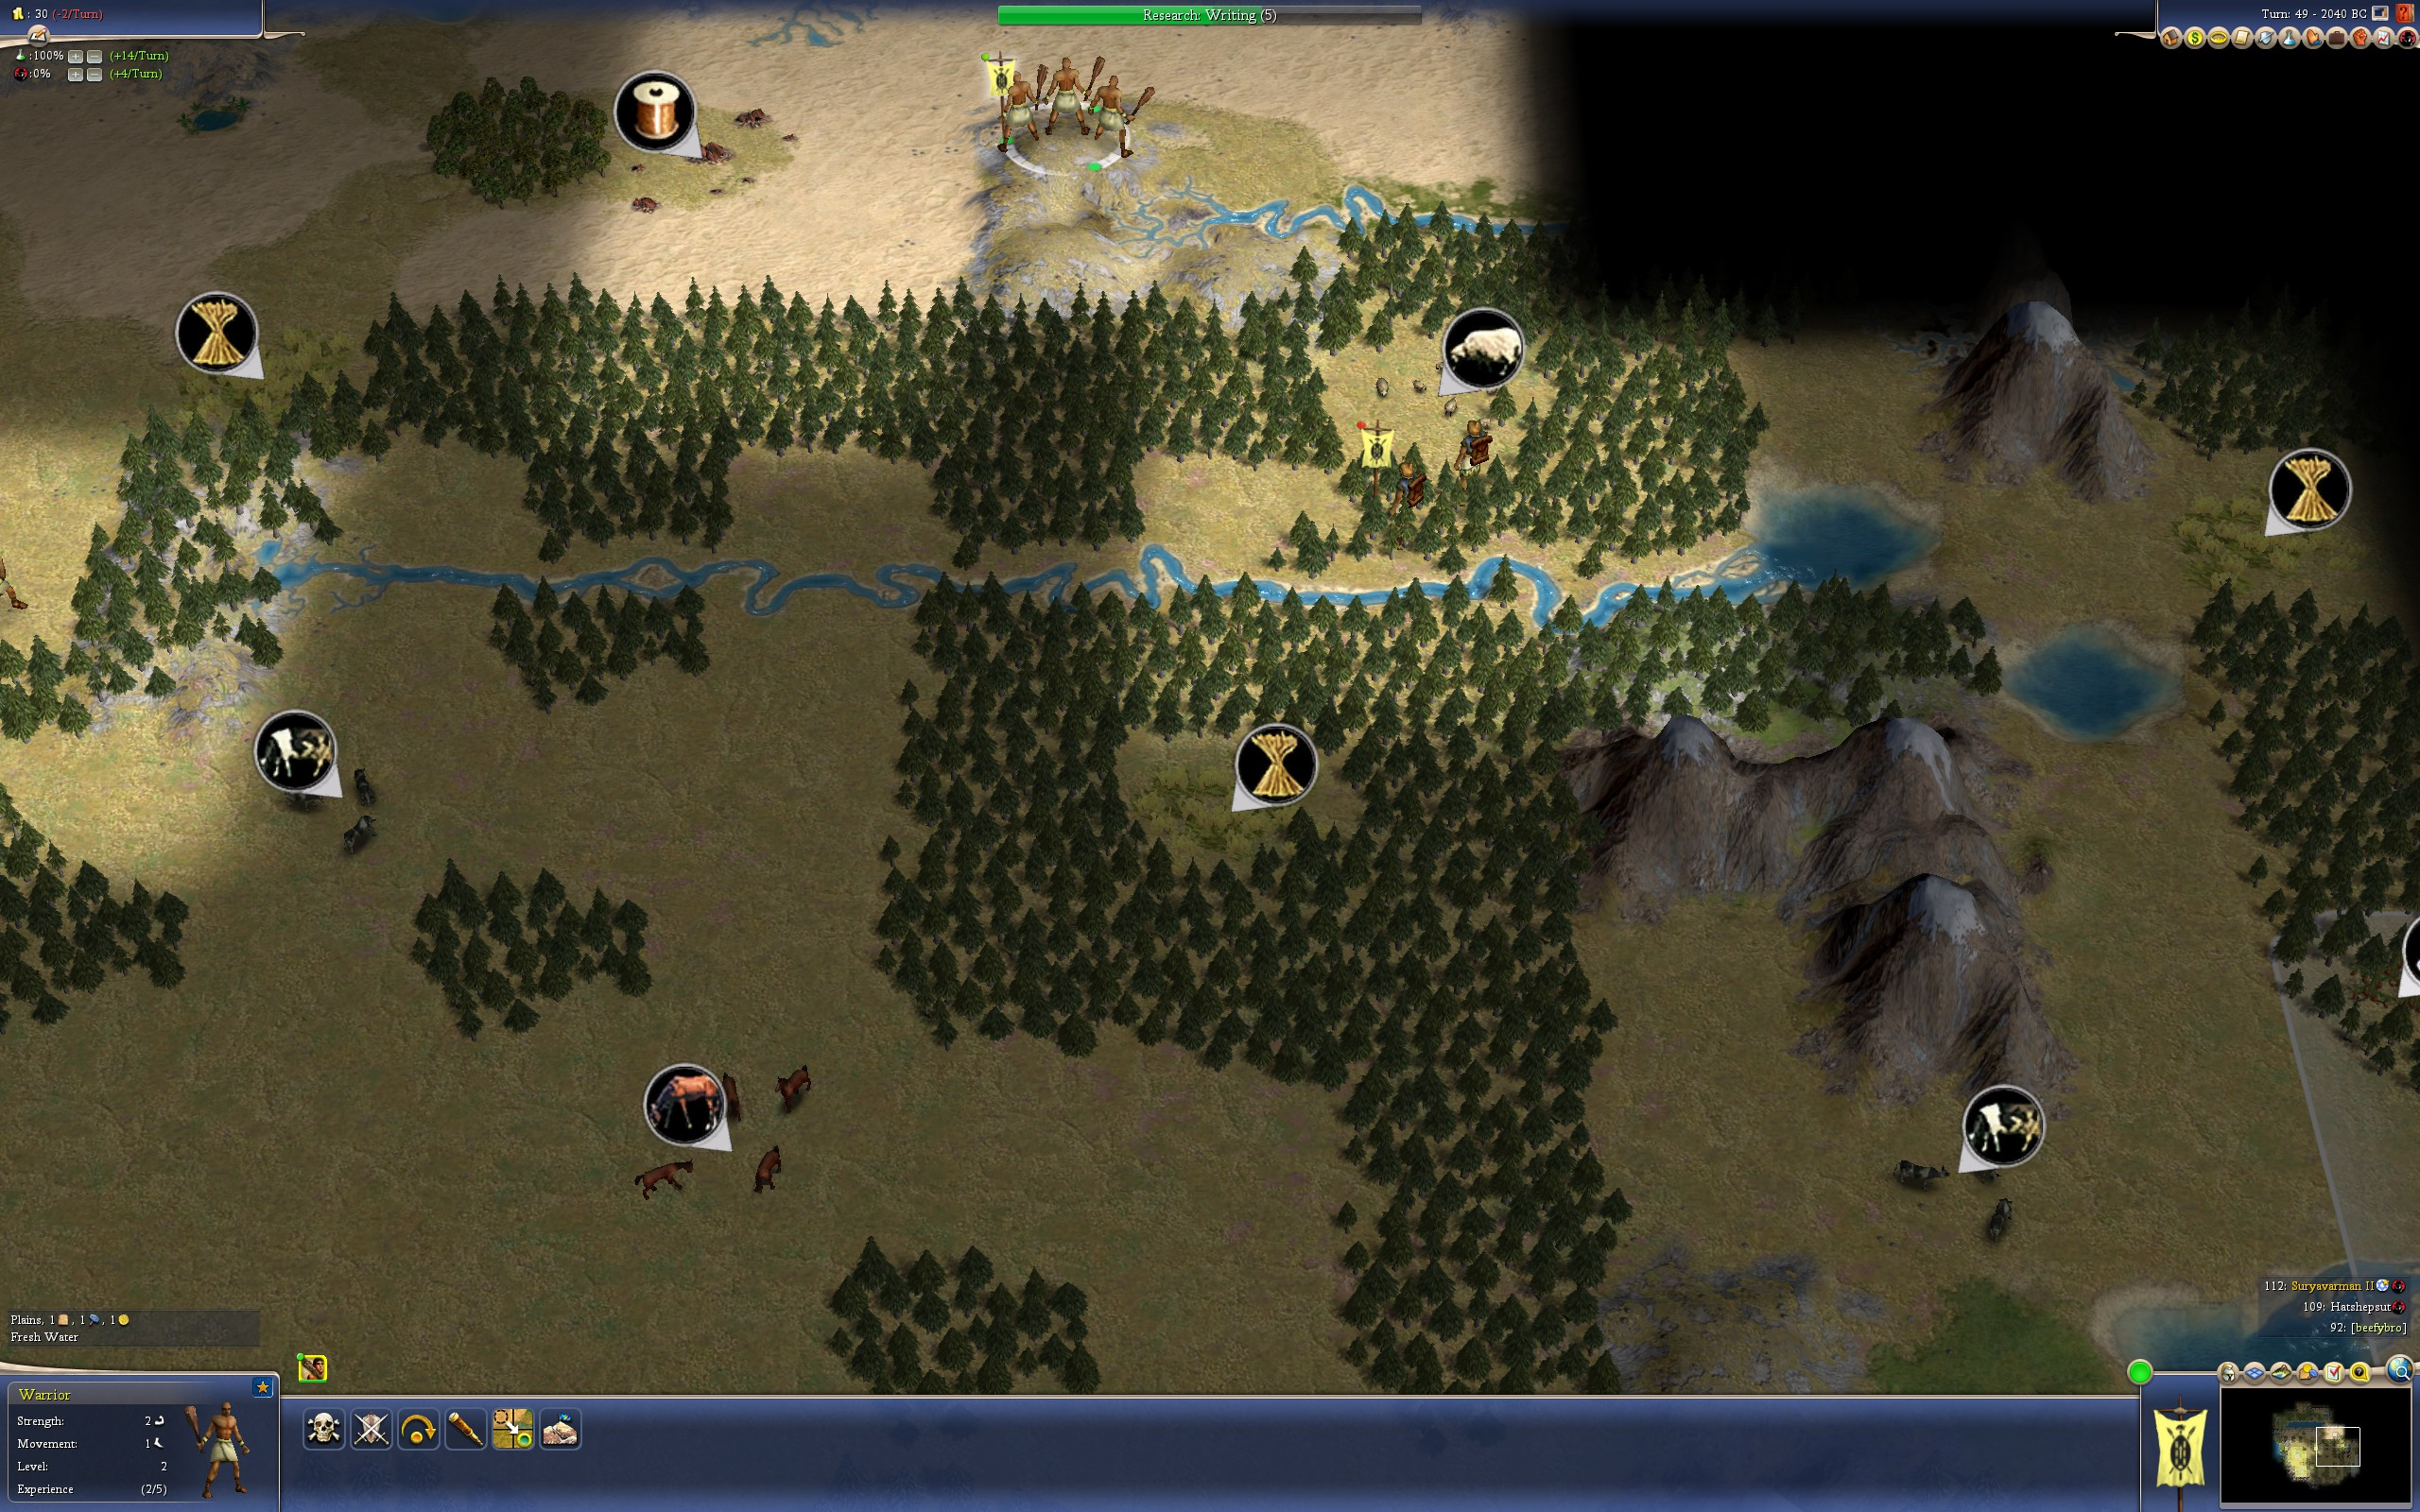
\includegraphics[width=1.0\textwidth]{22}

More decent land off to my east. I'm trying to \emph{fog bust} but there's way too much land to cover.
Barbs are going to spawn like crazy soon.

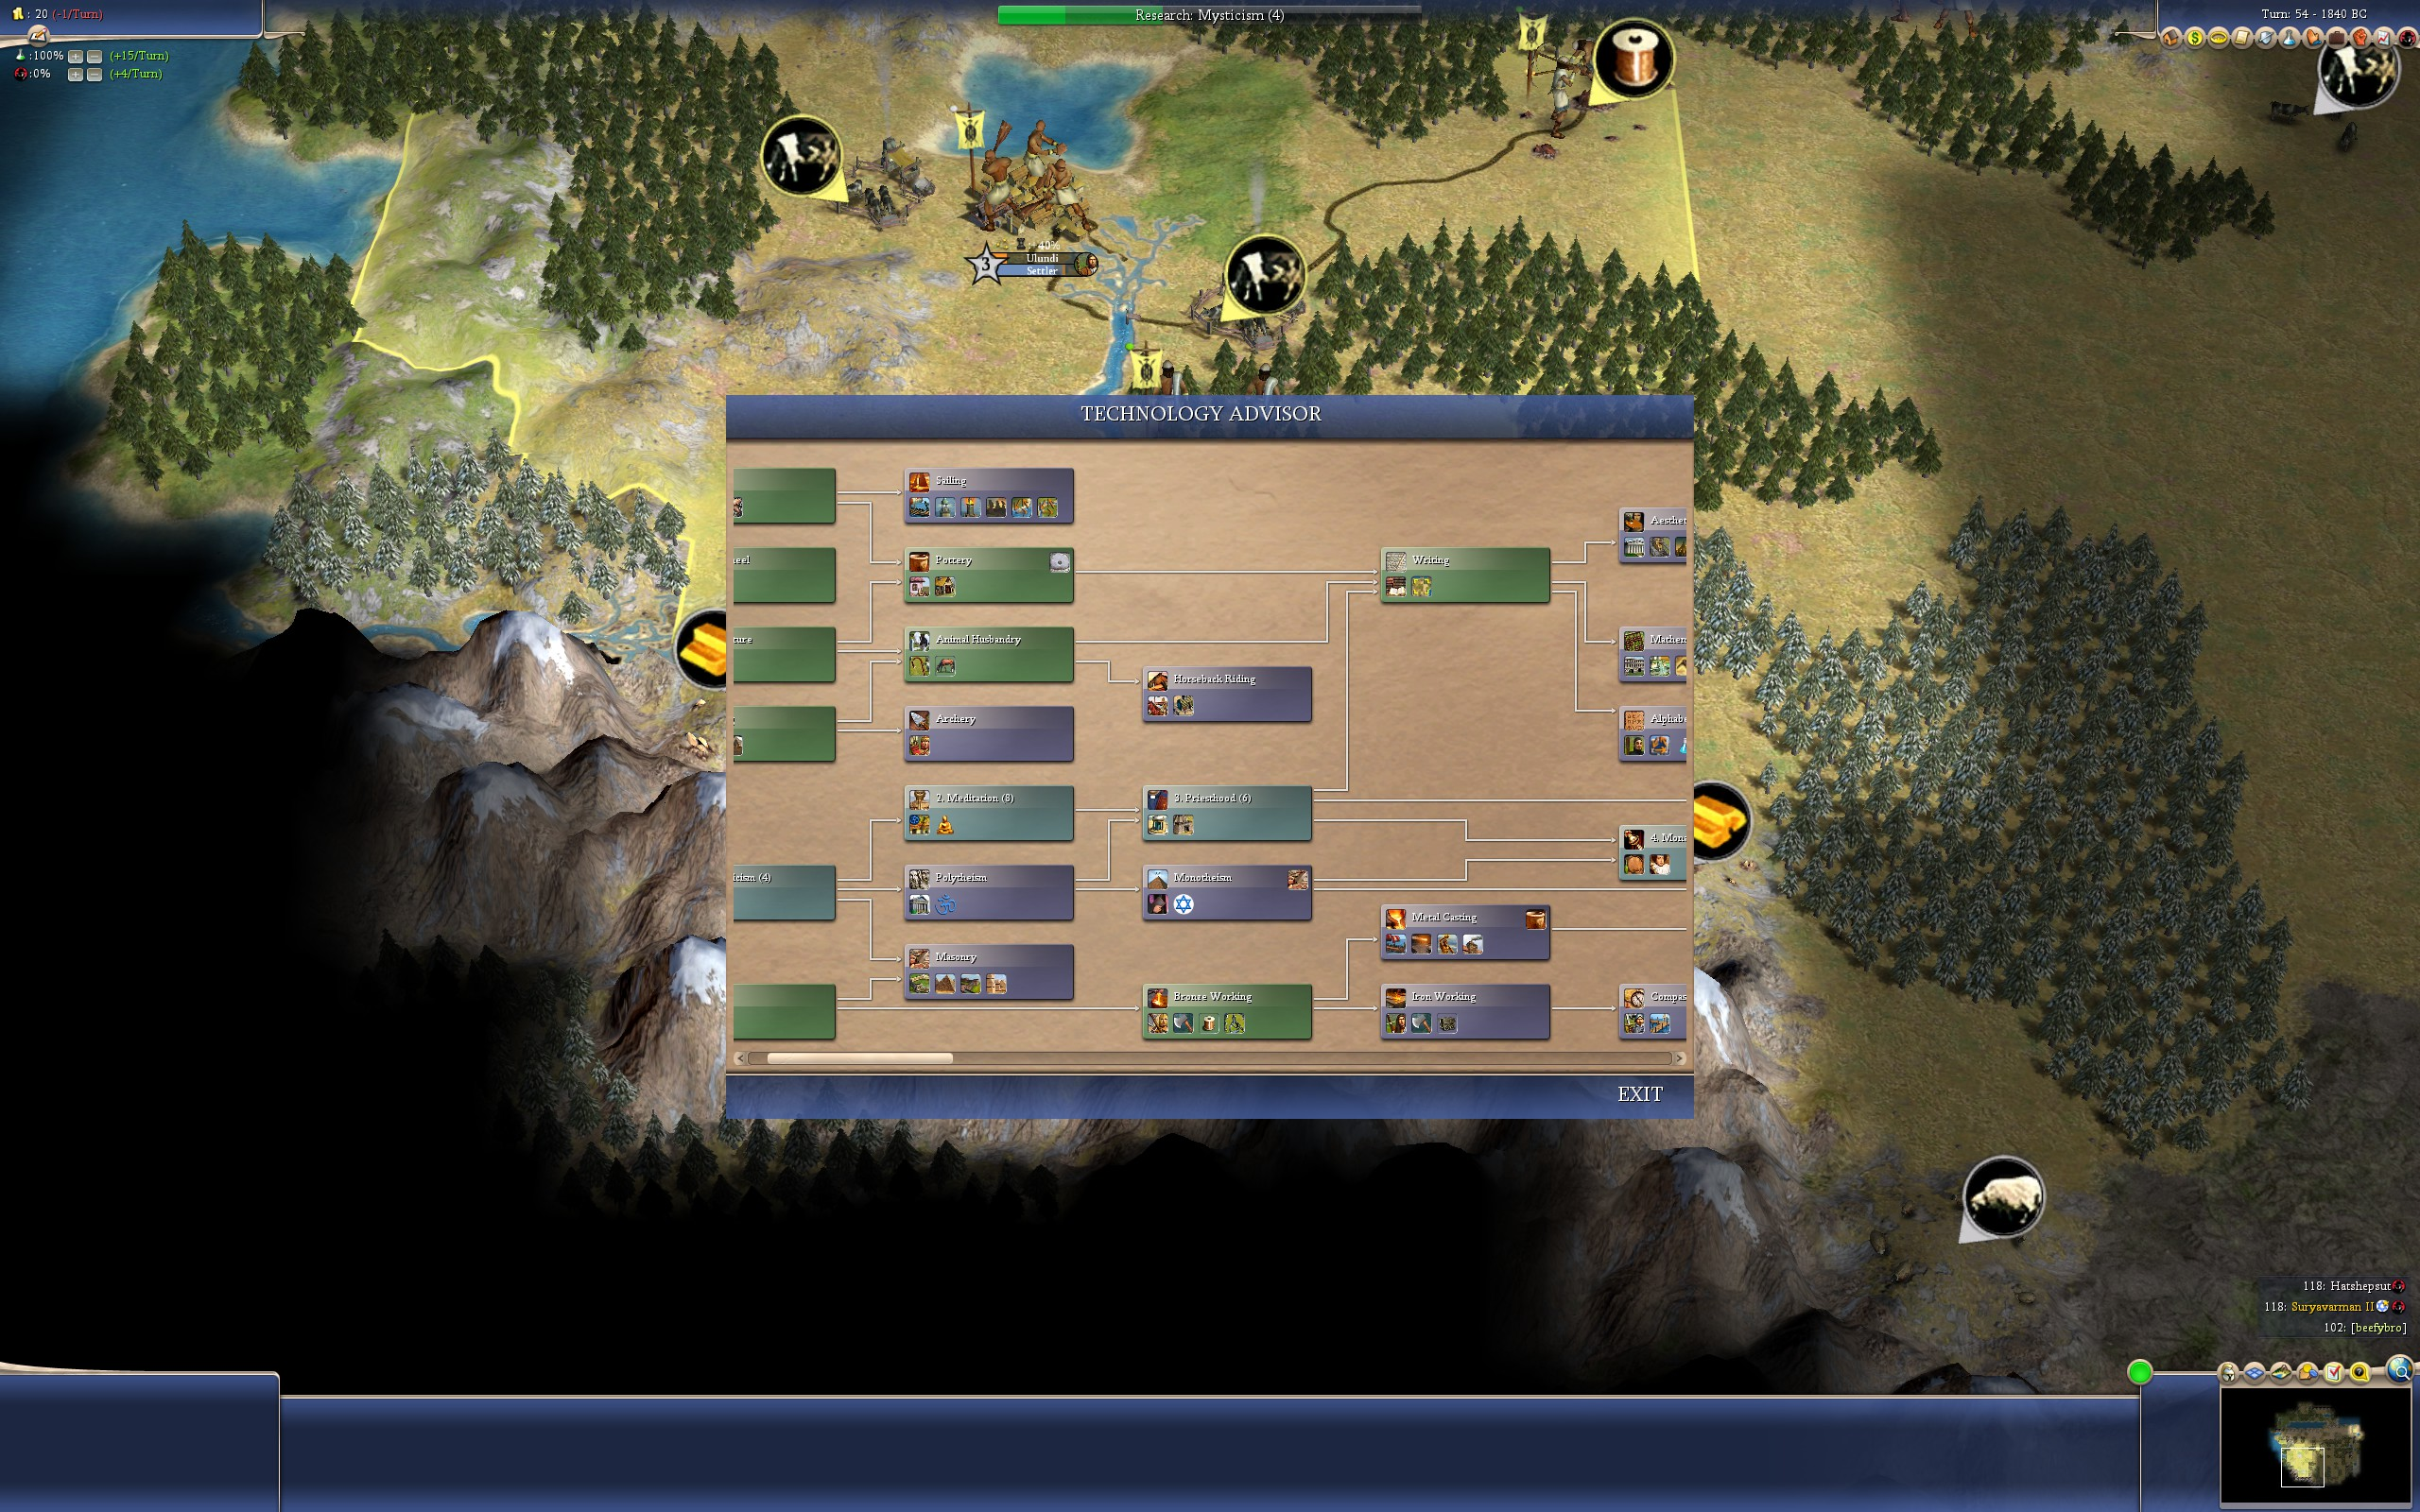
\includegraphics[width=1.0\textwidth]{23}

Writing complete, another tech choice to make. I've opted to fill-in some religious techs on the way to
Monarchy. This is not that strong of a play but there weren't any better choice. Sailing is an option but
I have no coastal cities and no water connections to other civs, so it does zip for me at this point. Monarchy
is always useful and religions should spread to me eventually.

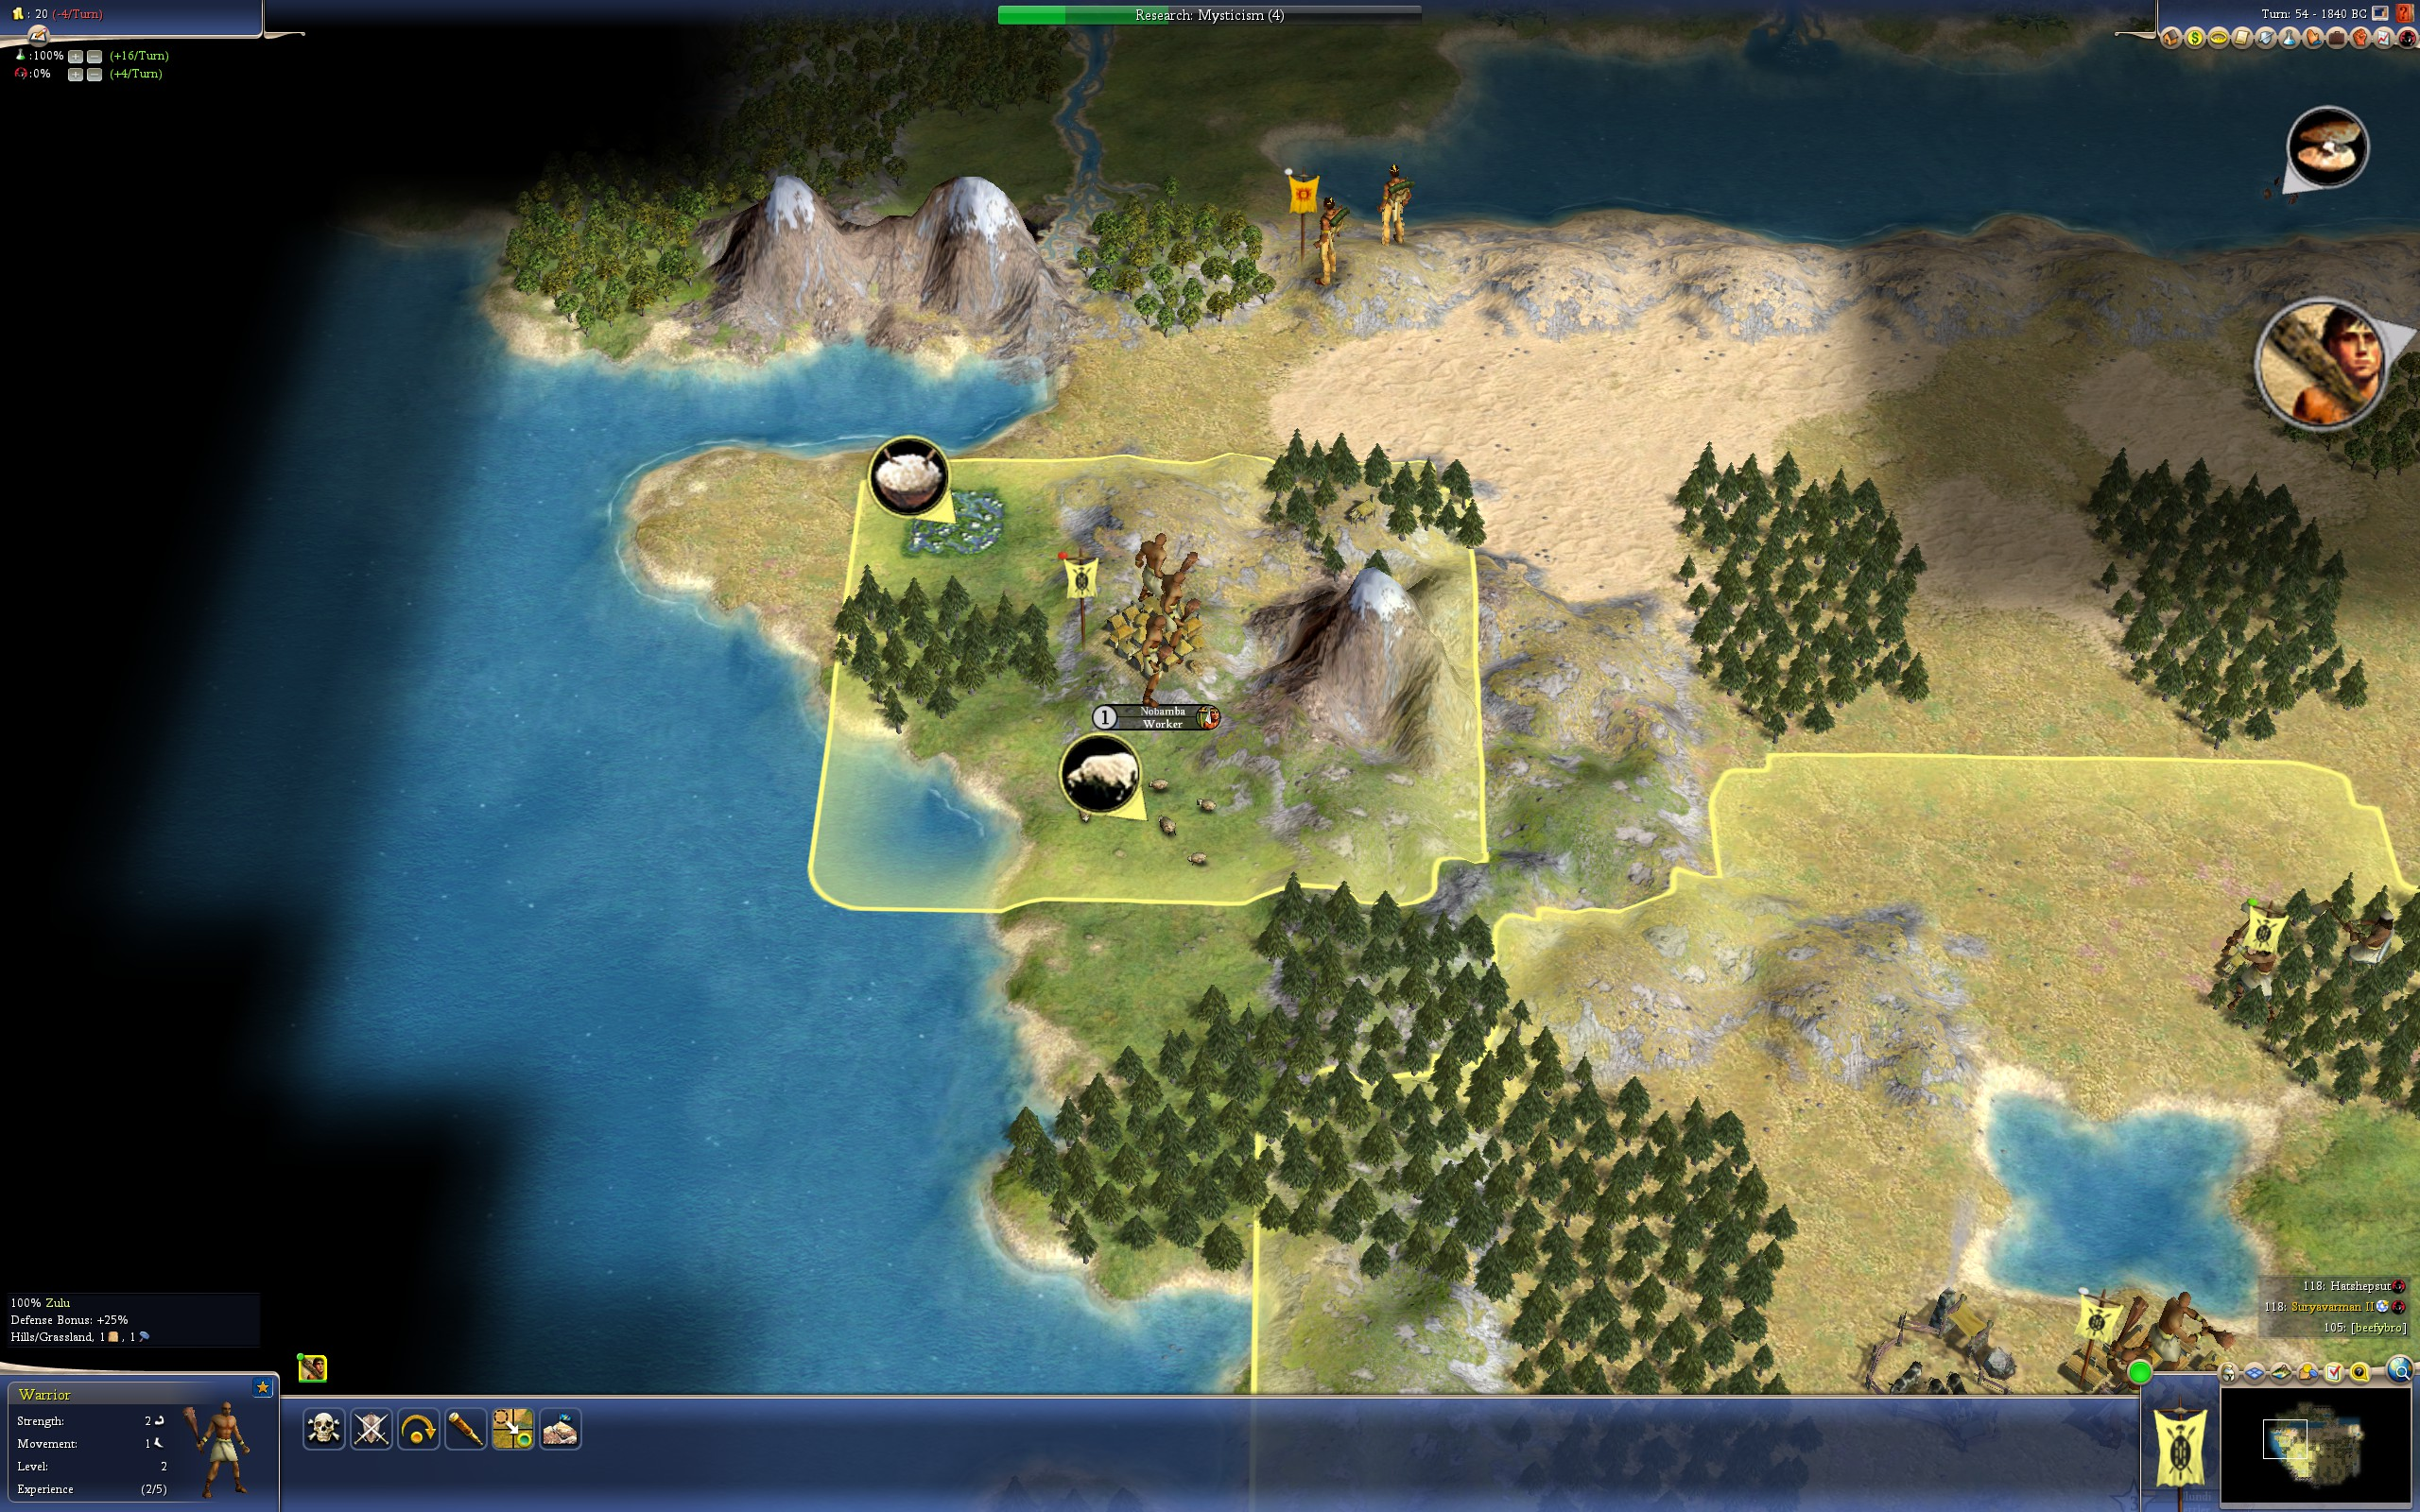
\includegraphics[width=1.0\textwidth]{24}

I've founded my 3rd city. Any city that has two food bonuses will be a good city. Normally, I would
have prioritized getting bronze, but the bronze is so close to my capital that I don't need to make
a city to get it; the capitals second culture pop will bring bronze into my borders.

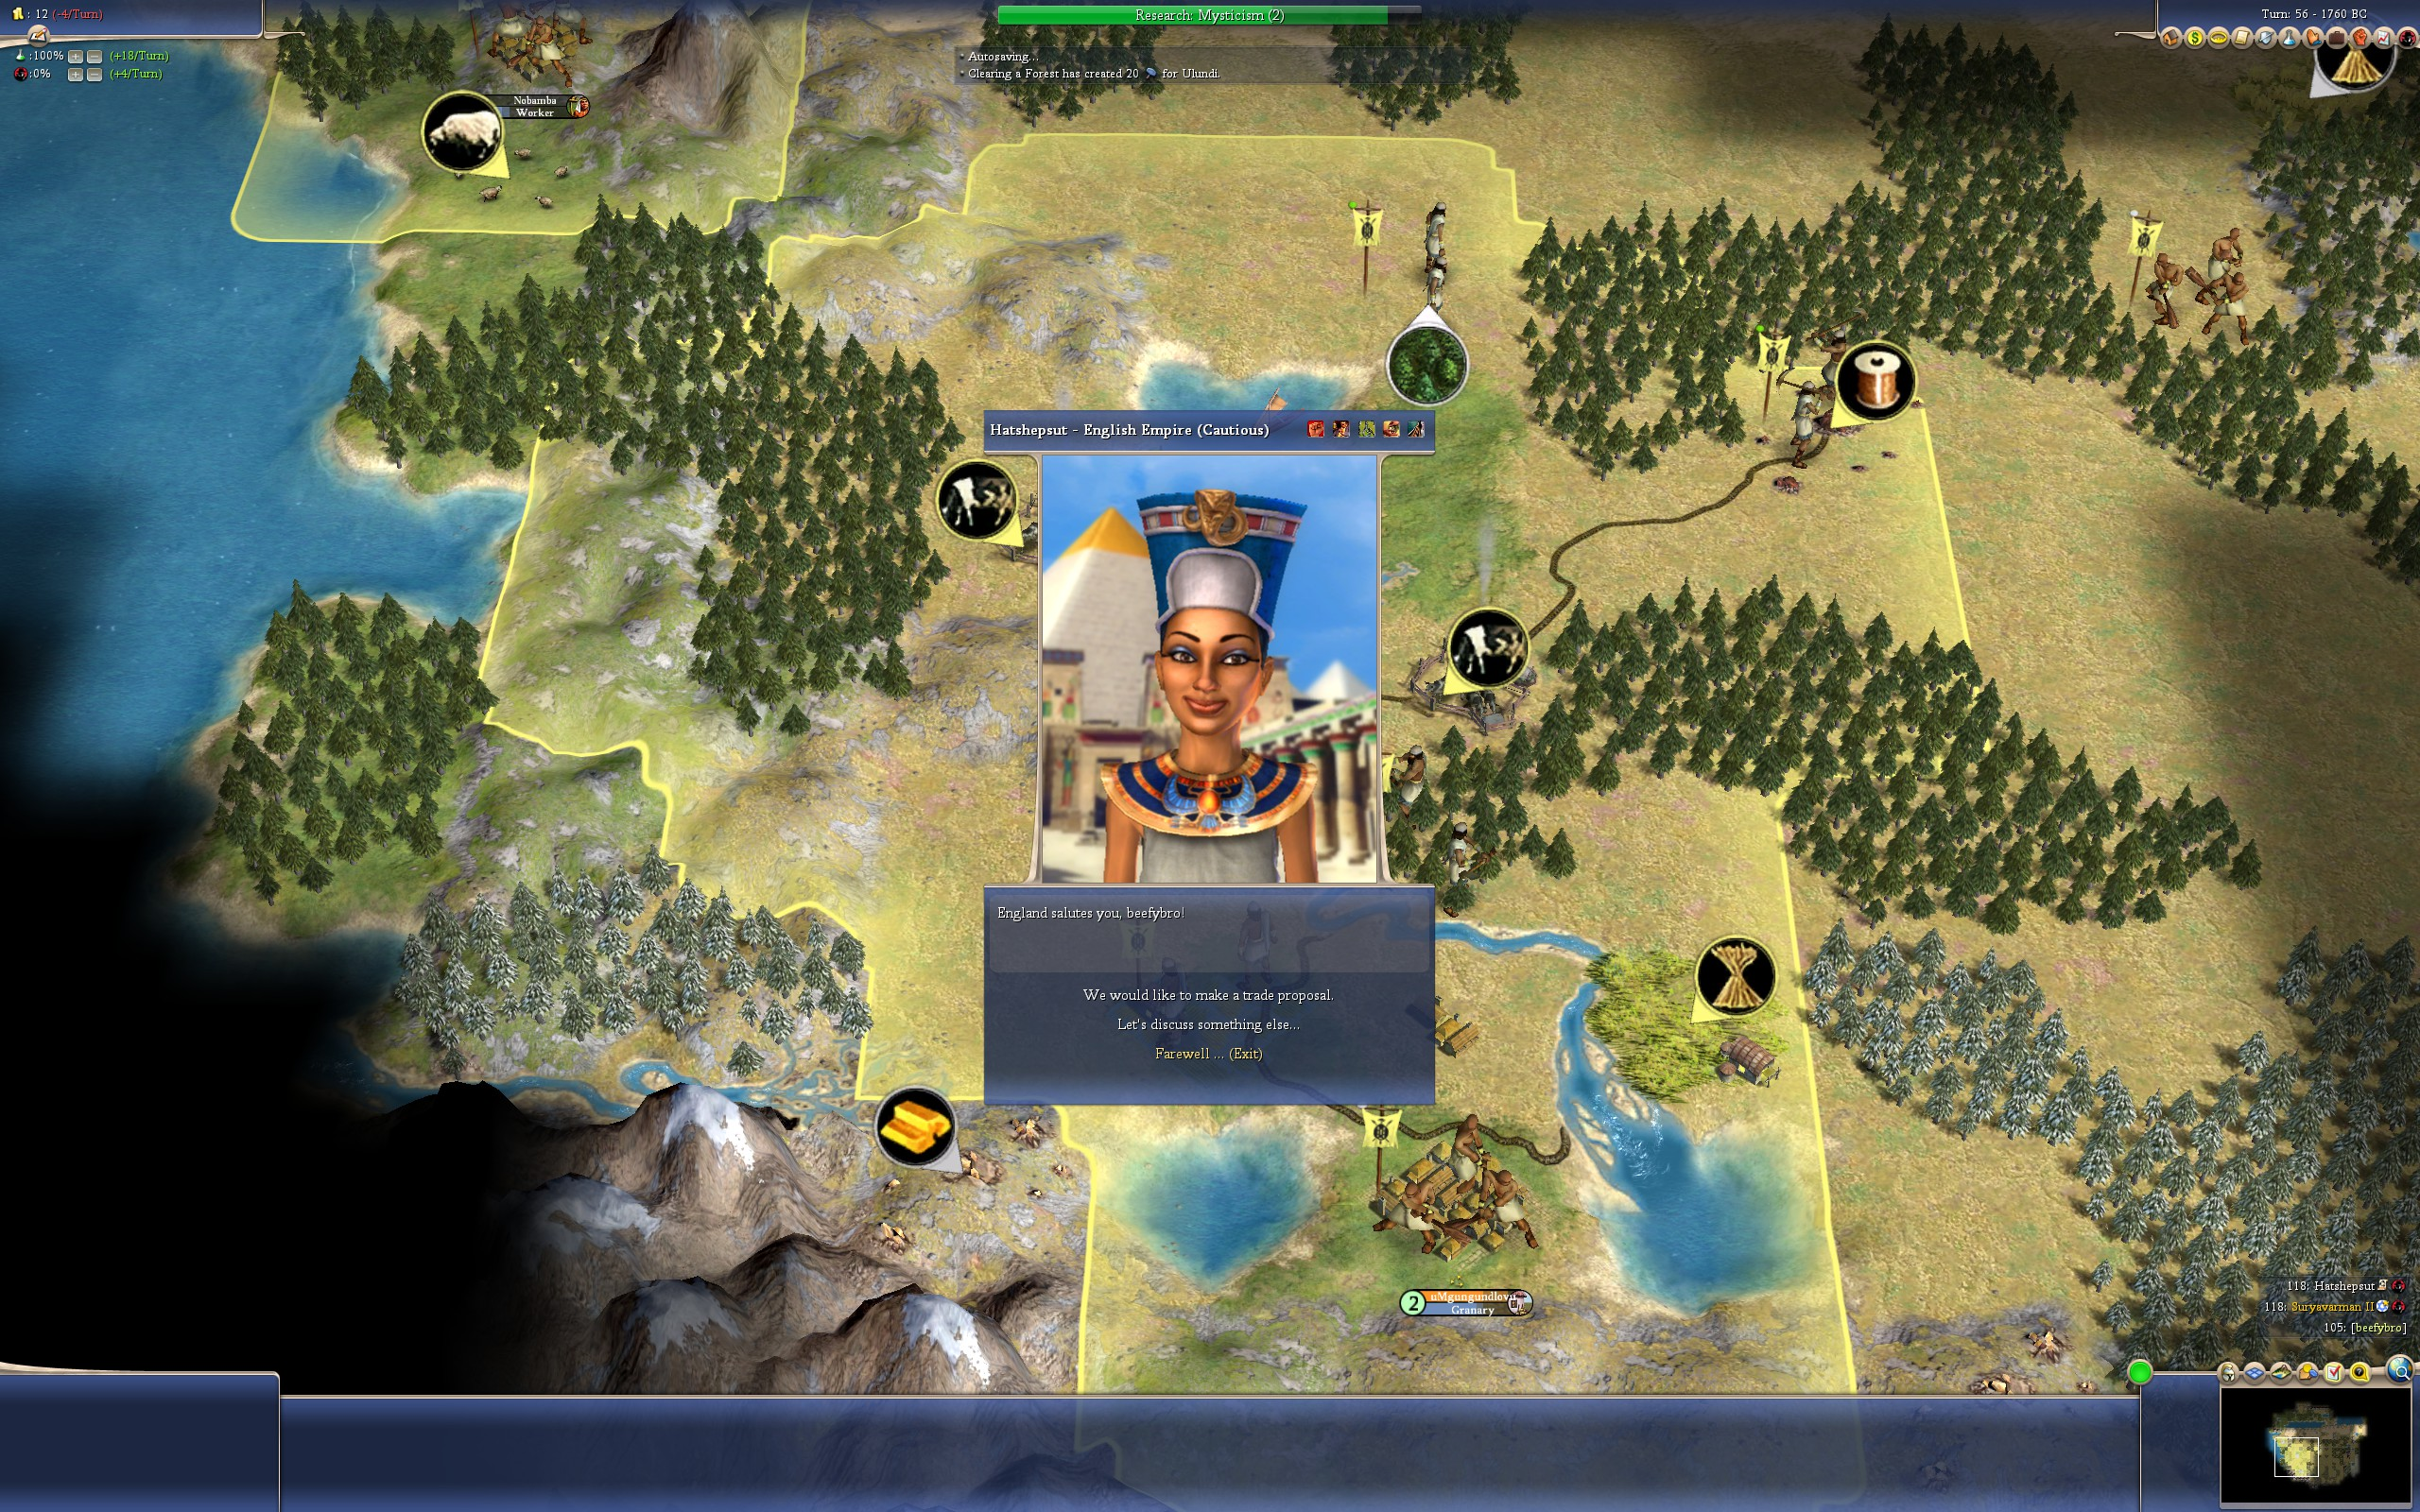
\includegraphics[width=1.0\textwidth]{25}

OB with Hatty signed. Getting trade routes to her is a high priority only behind grabbing contested land.
You should generally be assertive about getting OB with your neighbors and establishing trade routes and
resource trades. These are mutually beneficial arrangements that most players are happy to enter into.

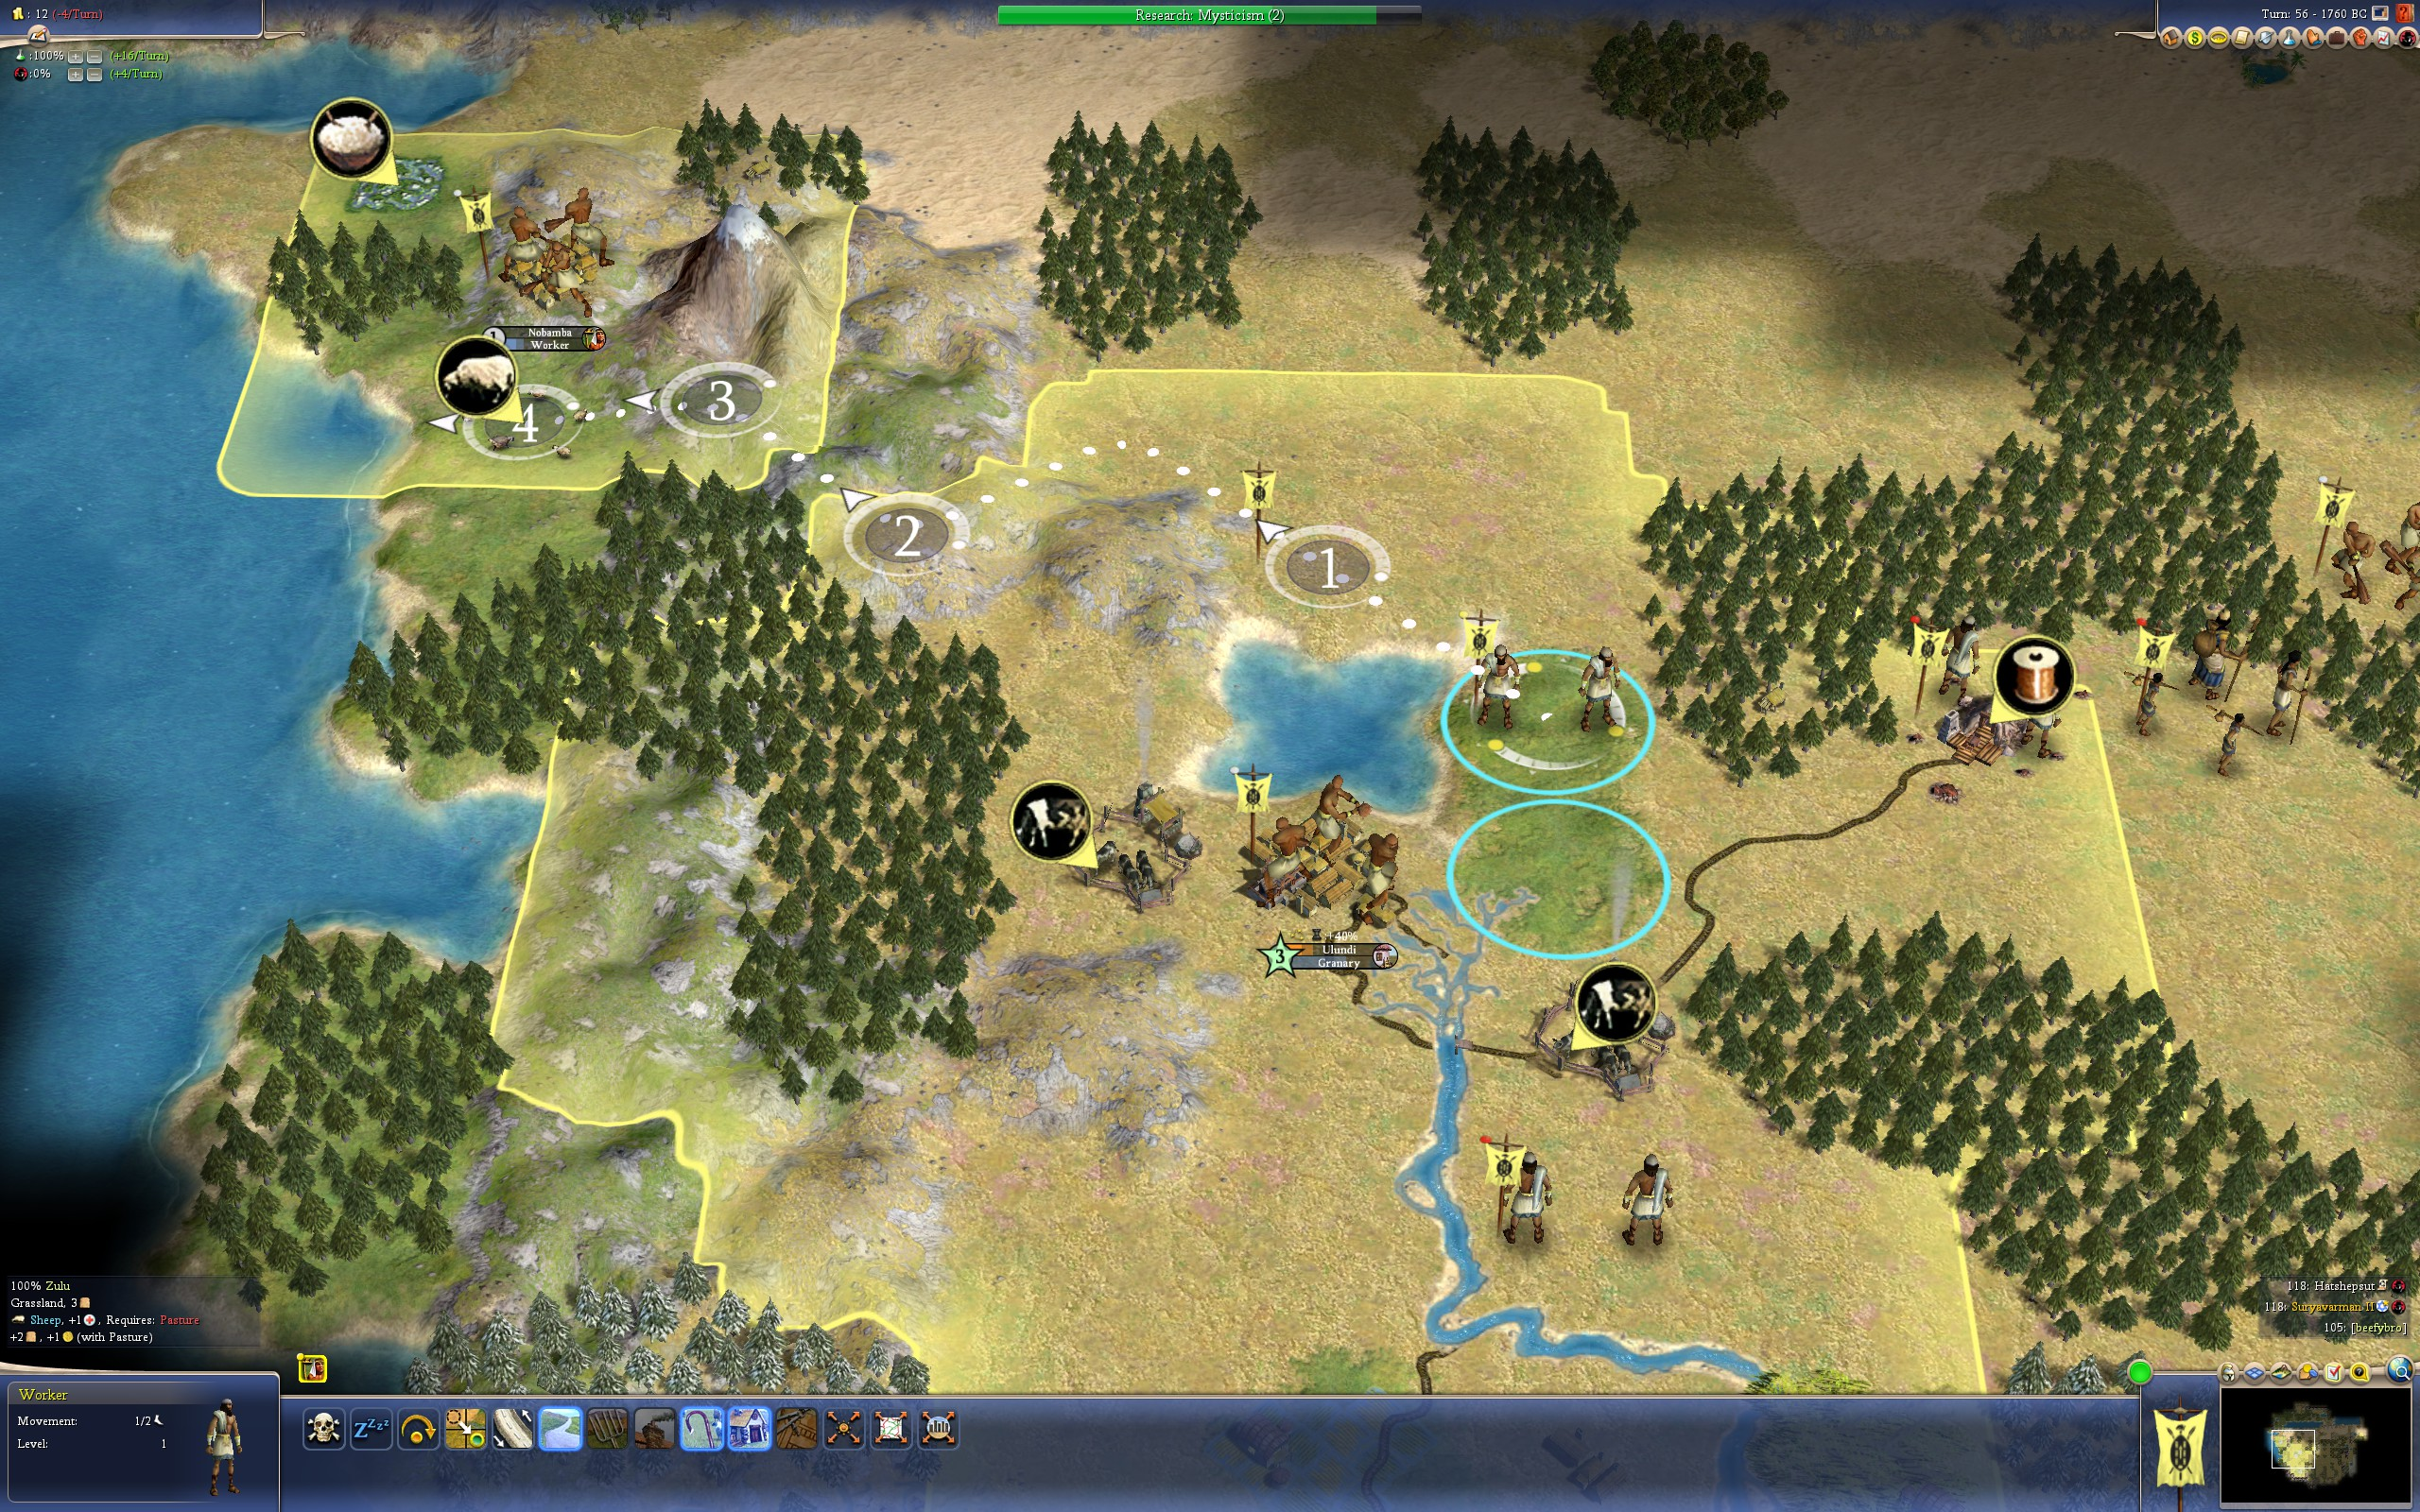
\includegraphics[width=1.0\textwidth]{26}

Once again, my surplus of workers allows me to loan a worker to a newly founded city which will accelerate
its development by at least 10-20 turns.

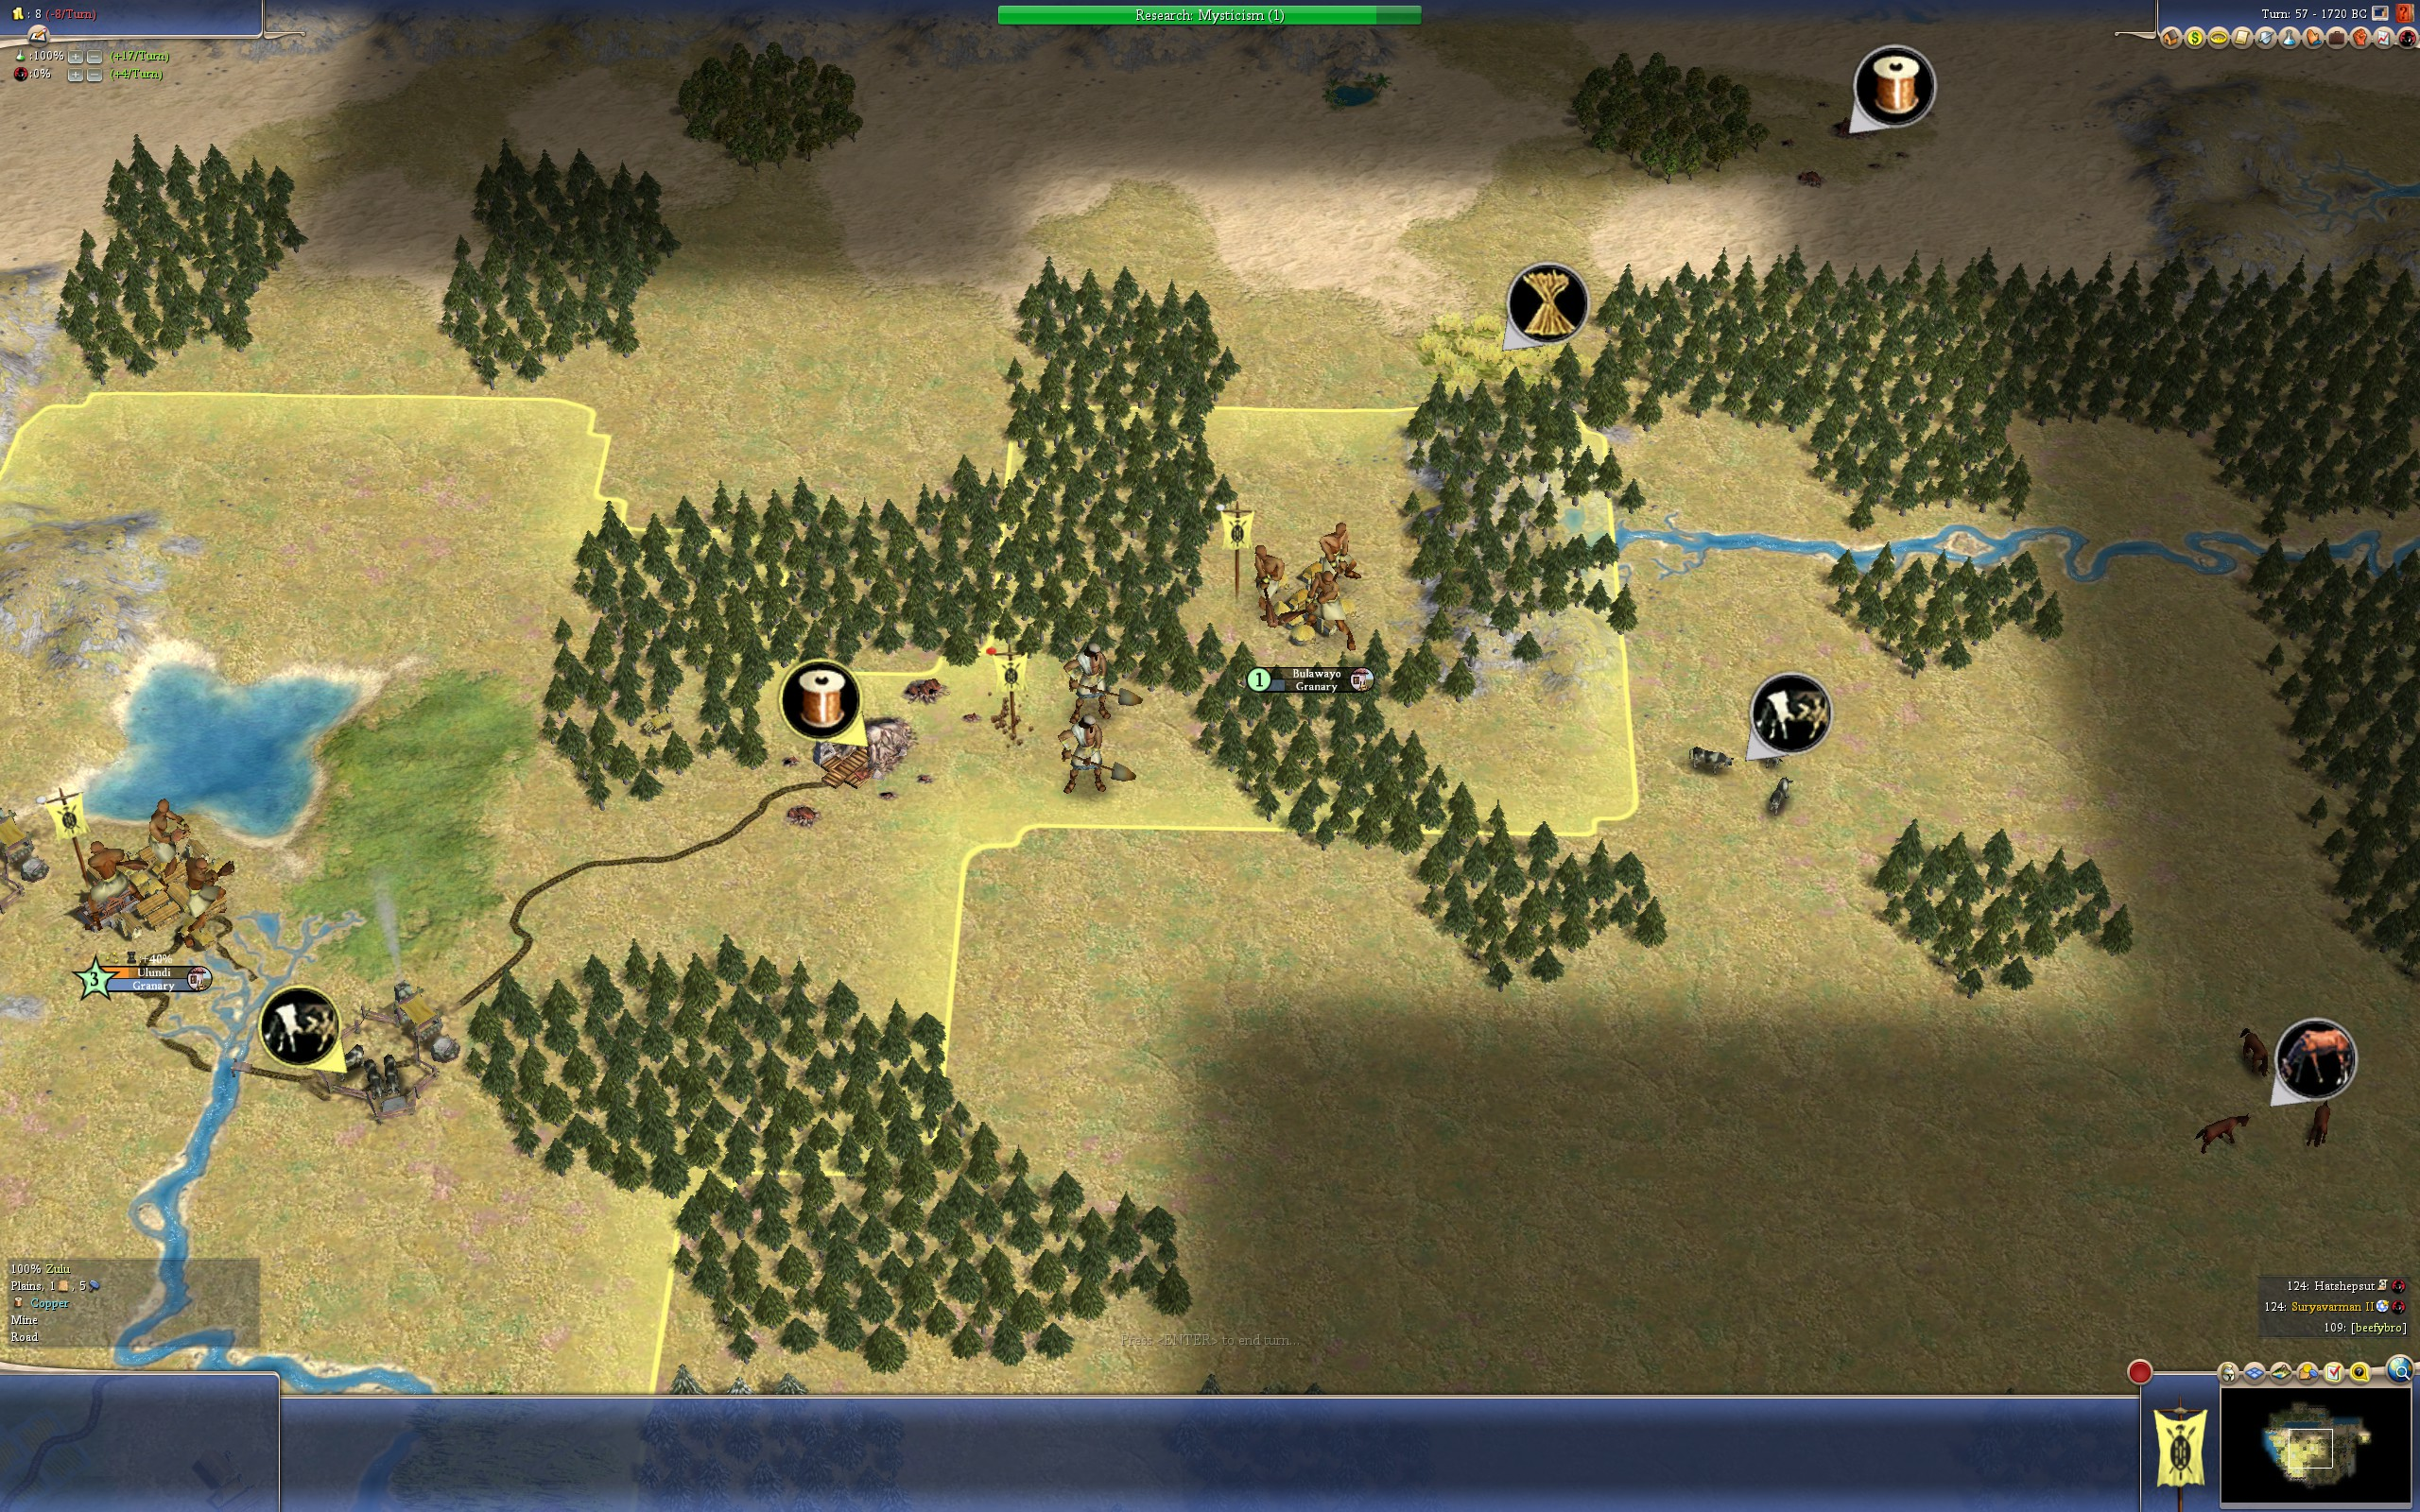
\includegraphics[width=1.0\textwidth]{27}

Bronze city goes down. It picks up two food nodes in addition to the bronze, but, yet again,
the number of brown (plains) tiles means this city will struggle for food. With barbs coming soon, I decide
to make this my military city for the early game. This city will work the bronze, cow, wheat, and a couple
mines to become an excellent production city. I can put these hammers into impis, my uber unit, and the barbs
then won't be a problem.

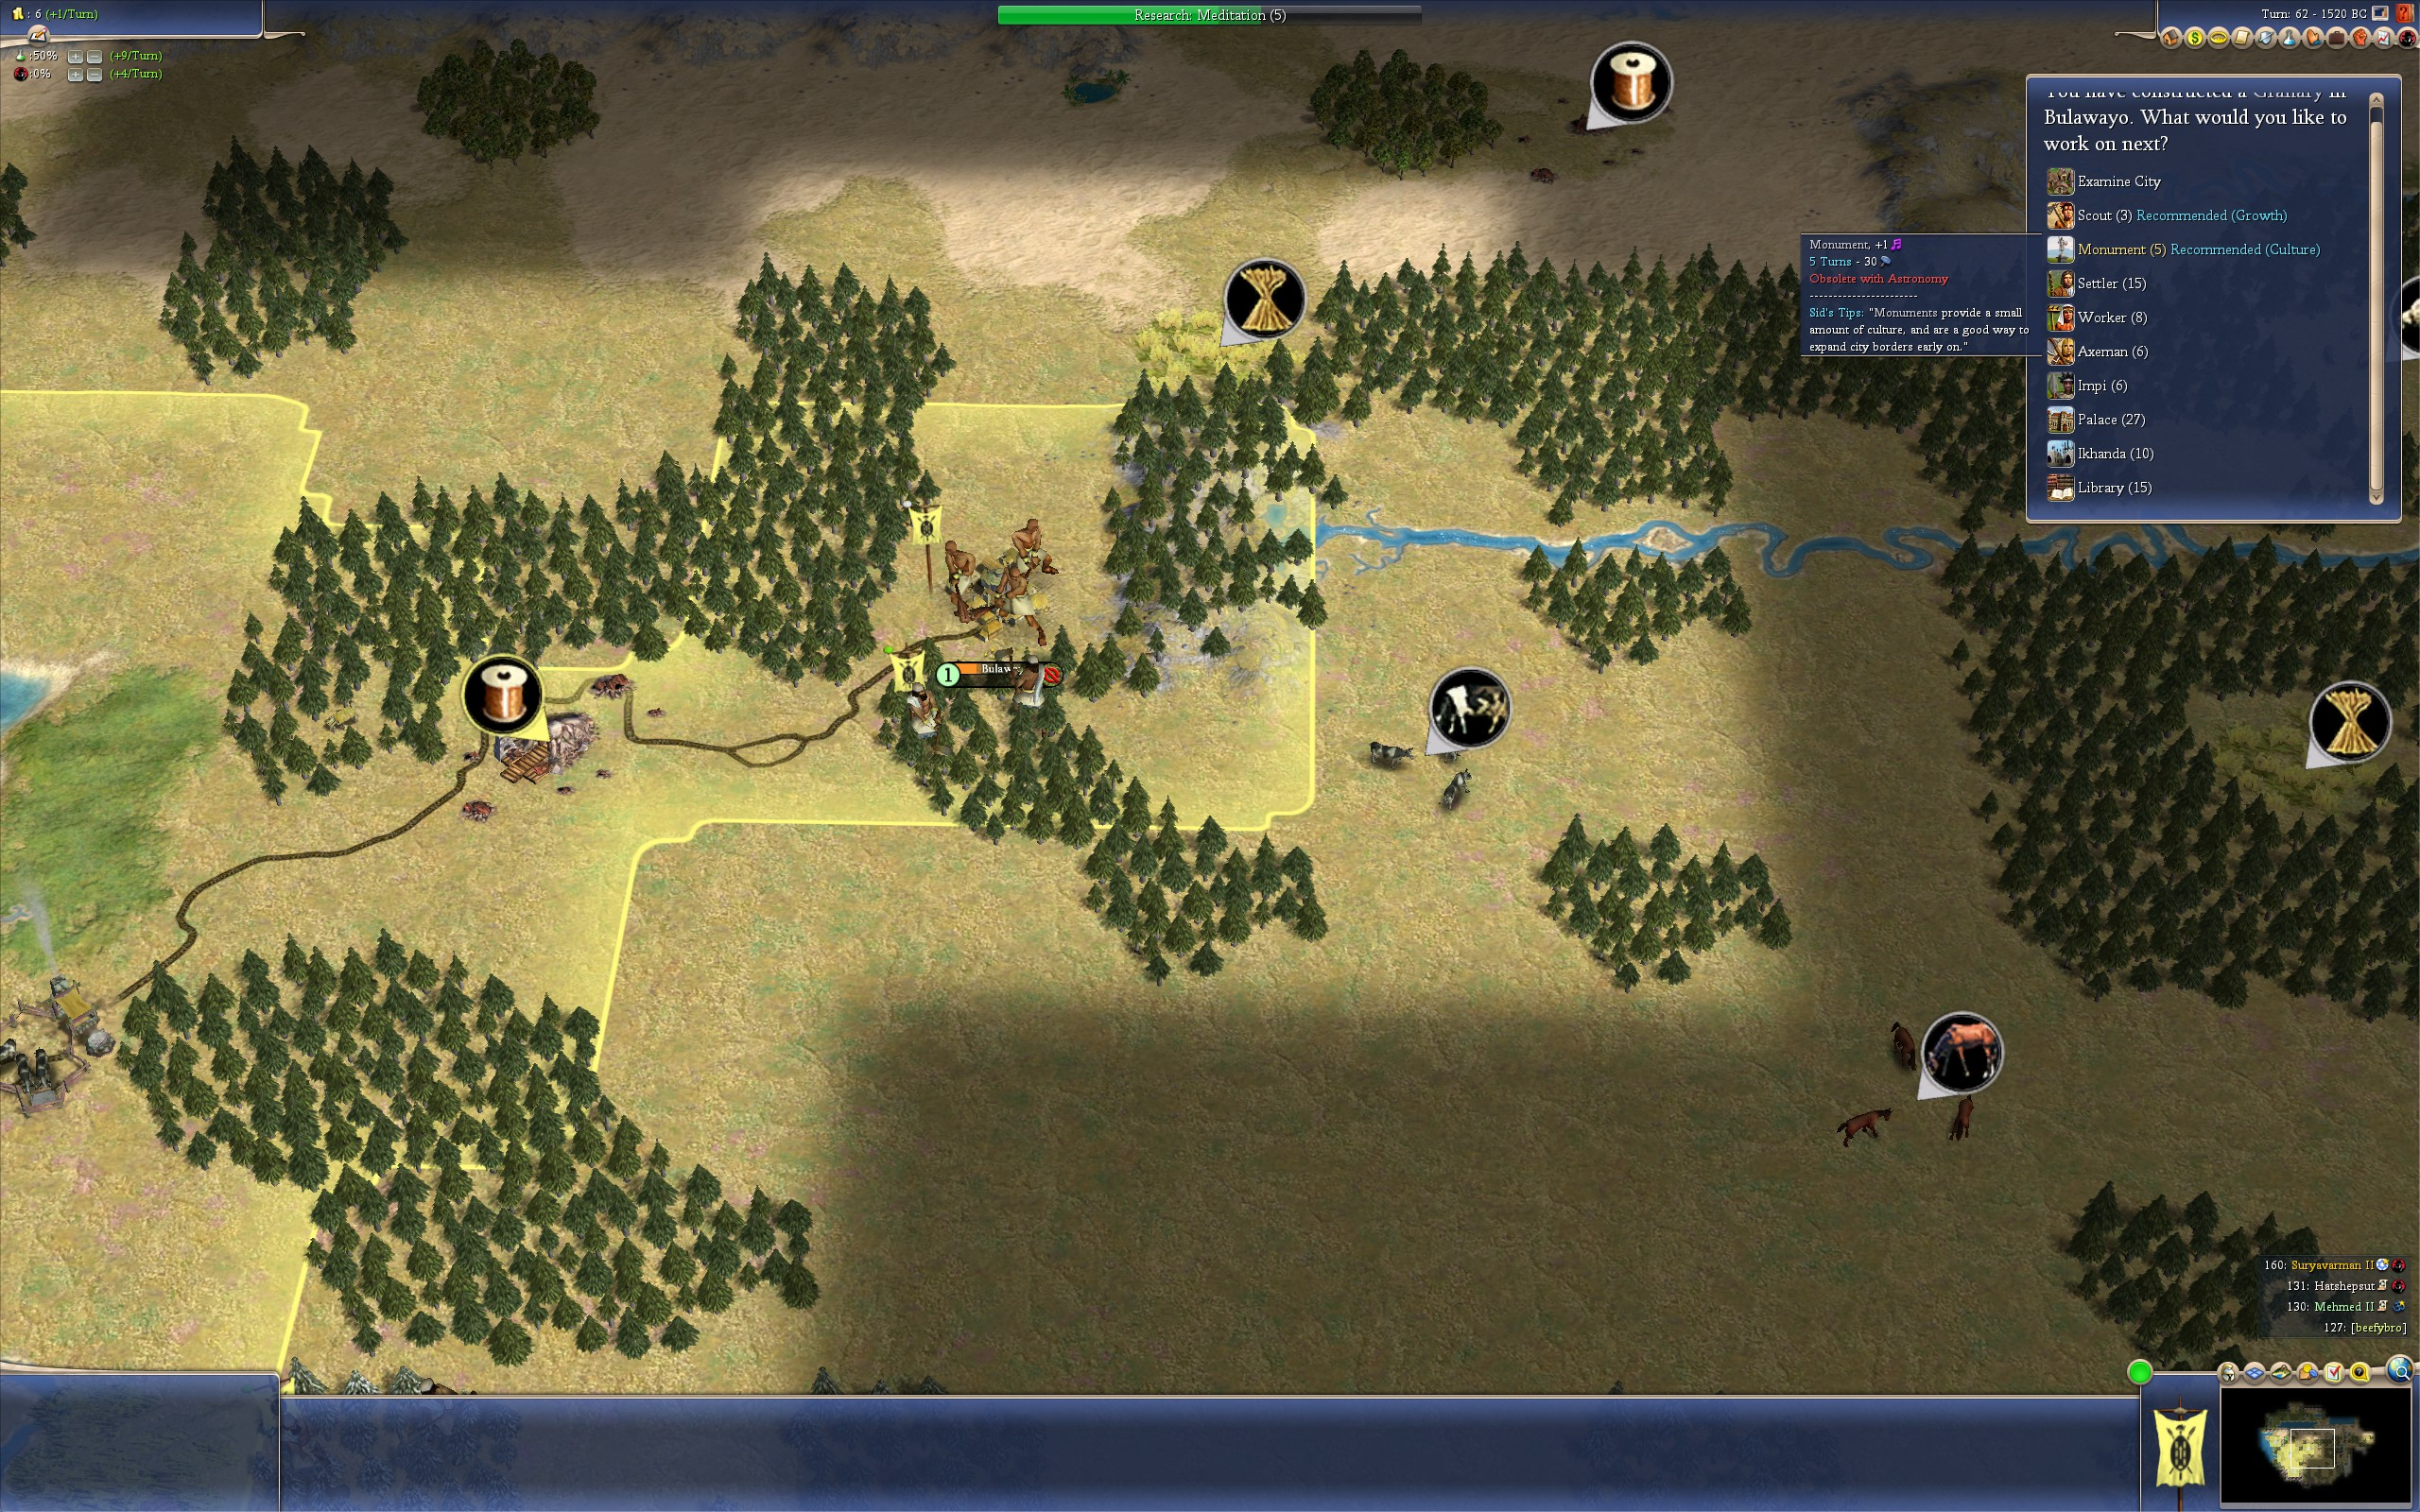
\includegraphics[width=1.0\textwidth]{30}

I really hate to build monuments unless I'm charismatic. In cities that are heavily forested, I sometimes
chop-out a library and skip the monument, but it this case the city is going to be extremely low commerce,
so monument it is. If you aren't charismatic, you should consider ways that enable you to skip monuments:
religions, libraries, creative leader, stonehenge.

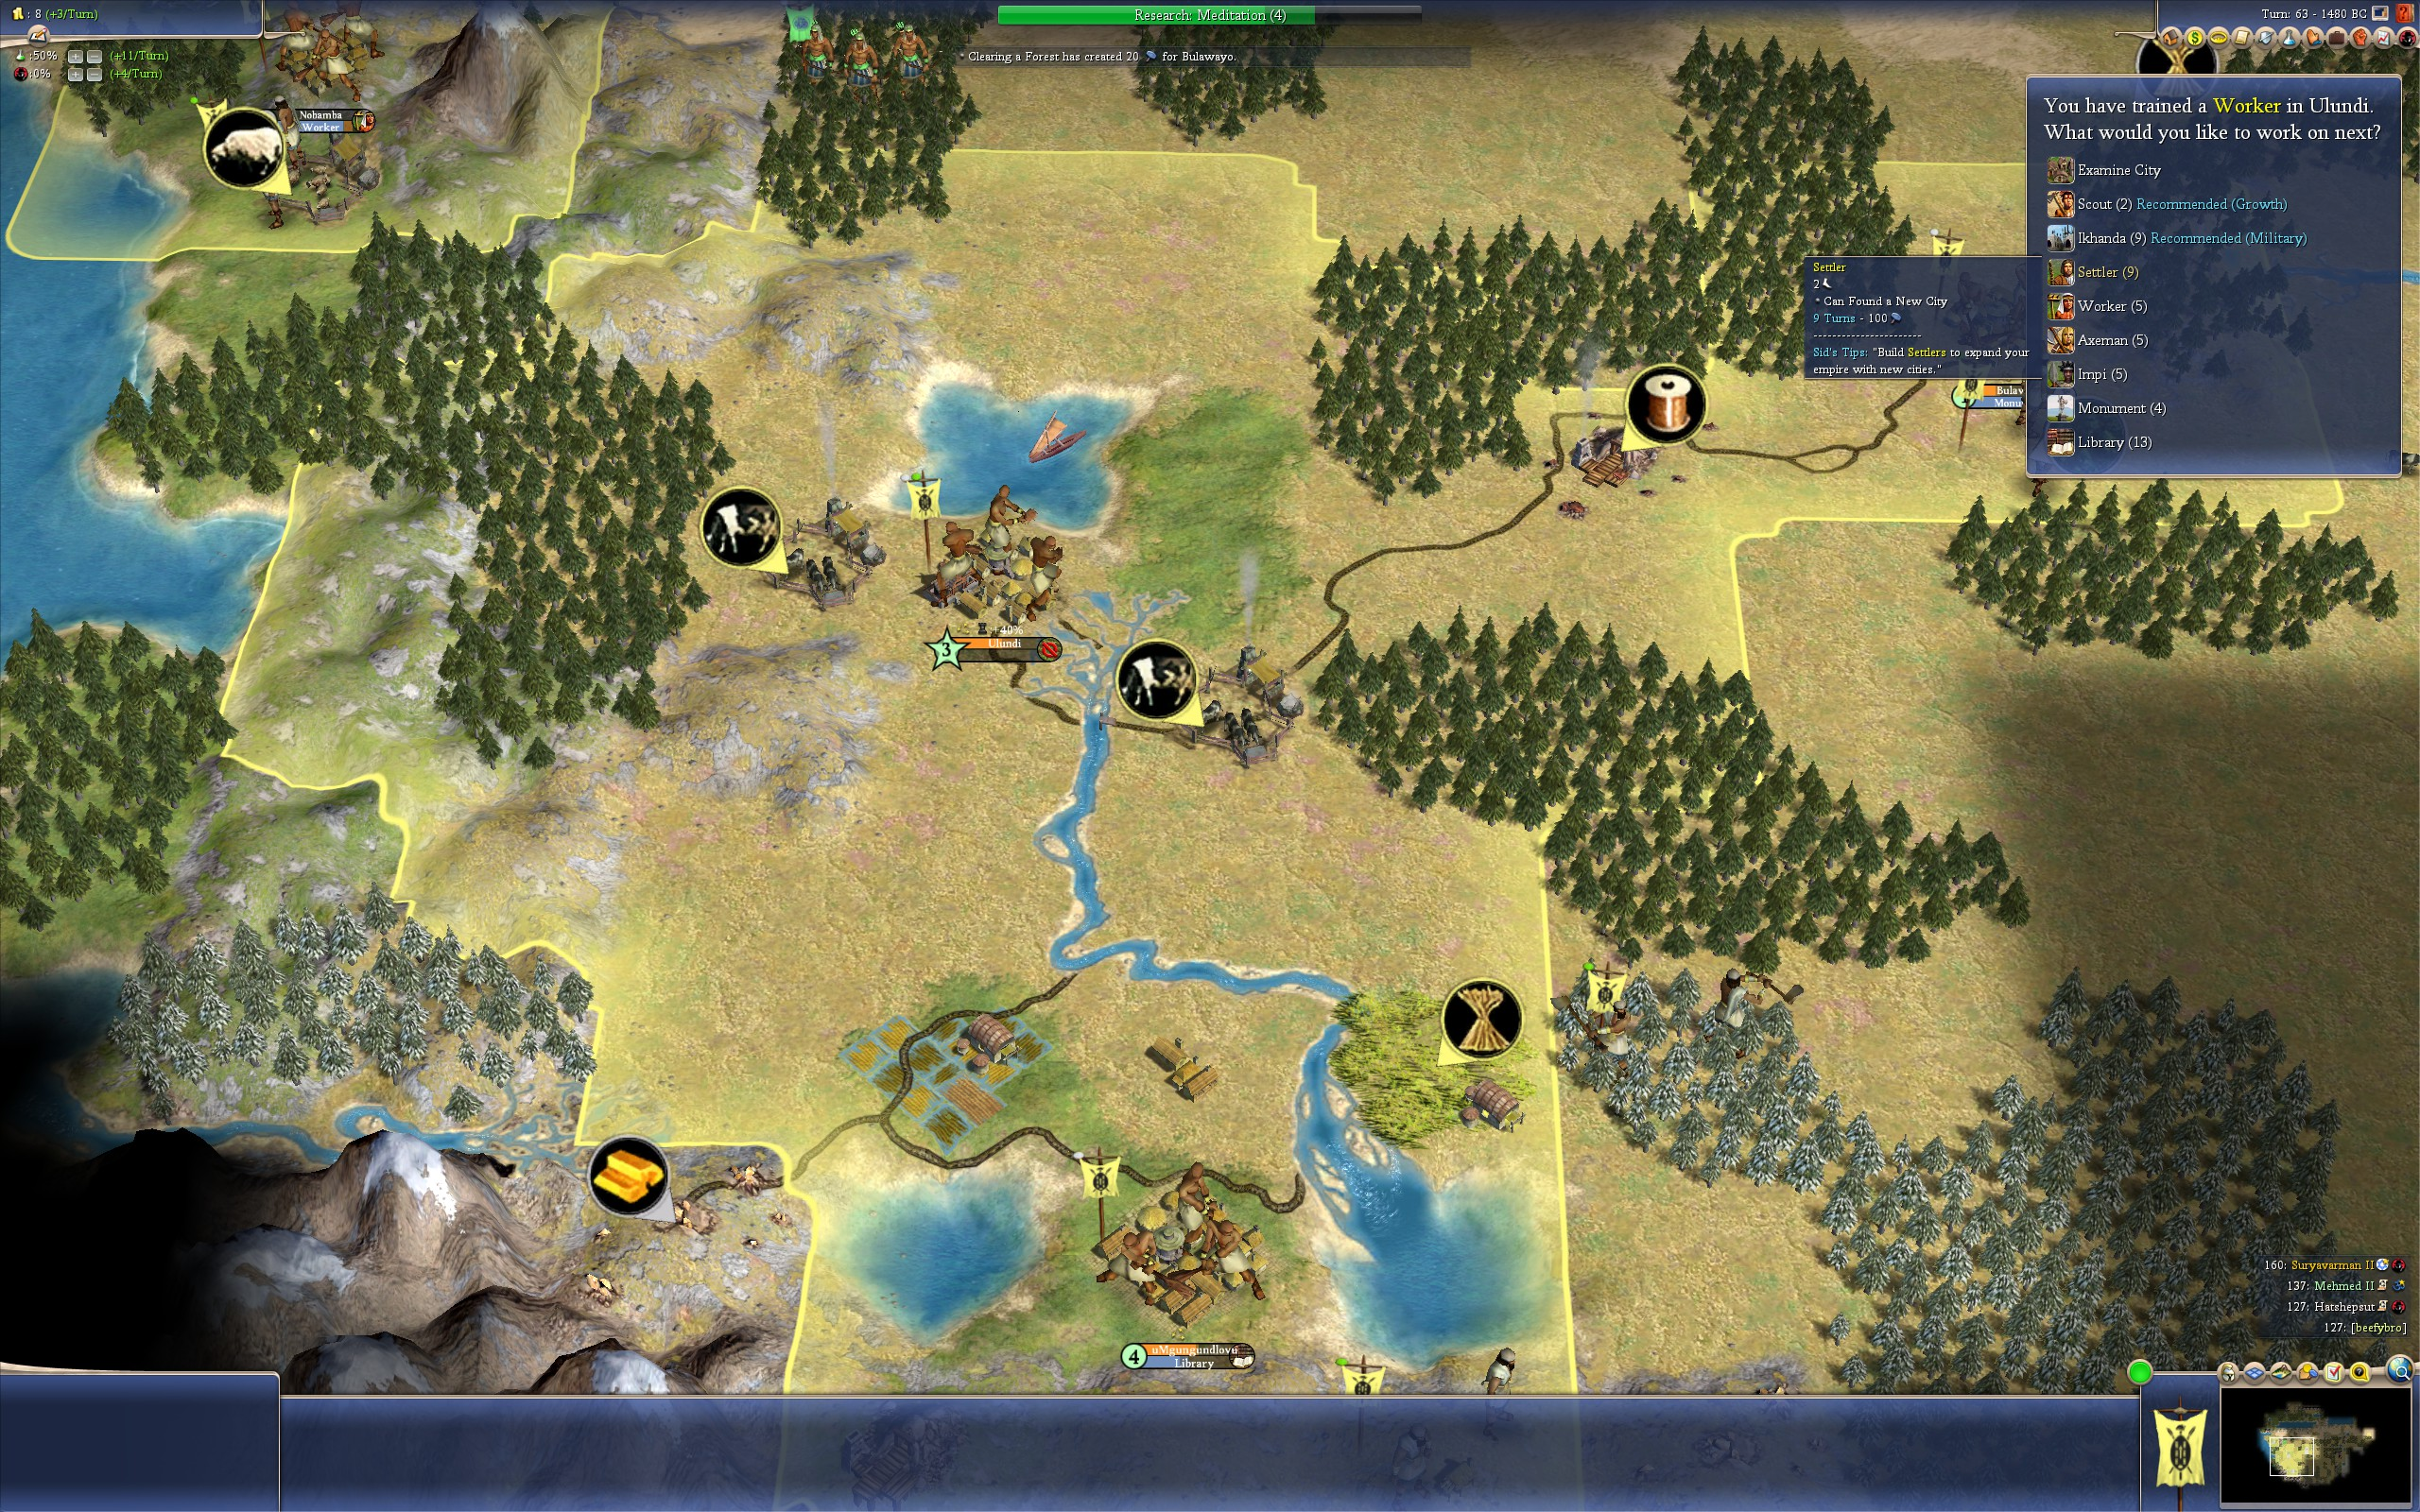
\includegraphics[width=1.0\textwidth]{31}

Couple things in this shot. My gold city is slowly building a library so that it can generate culture and
finally work the golds. This was clearly a mistake; a monument should have been built prior to the library.
The worker 2E 1N of gold city is also demonstrating a technique that's important: chopping outside a city's
borders. The hammers are slightly reduced for being outside borders, but hammers are so precious that it's
still well worth the effort. Same goes for forests outside a city's BFC, they should still be chopped. I
often see less-skilled players leaving lots of forests around their land; this is a mistake.

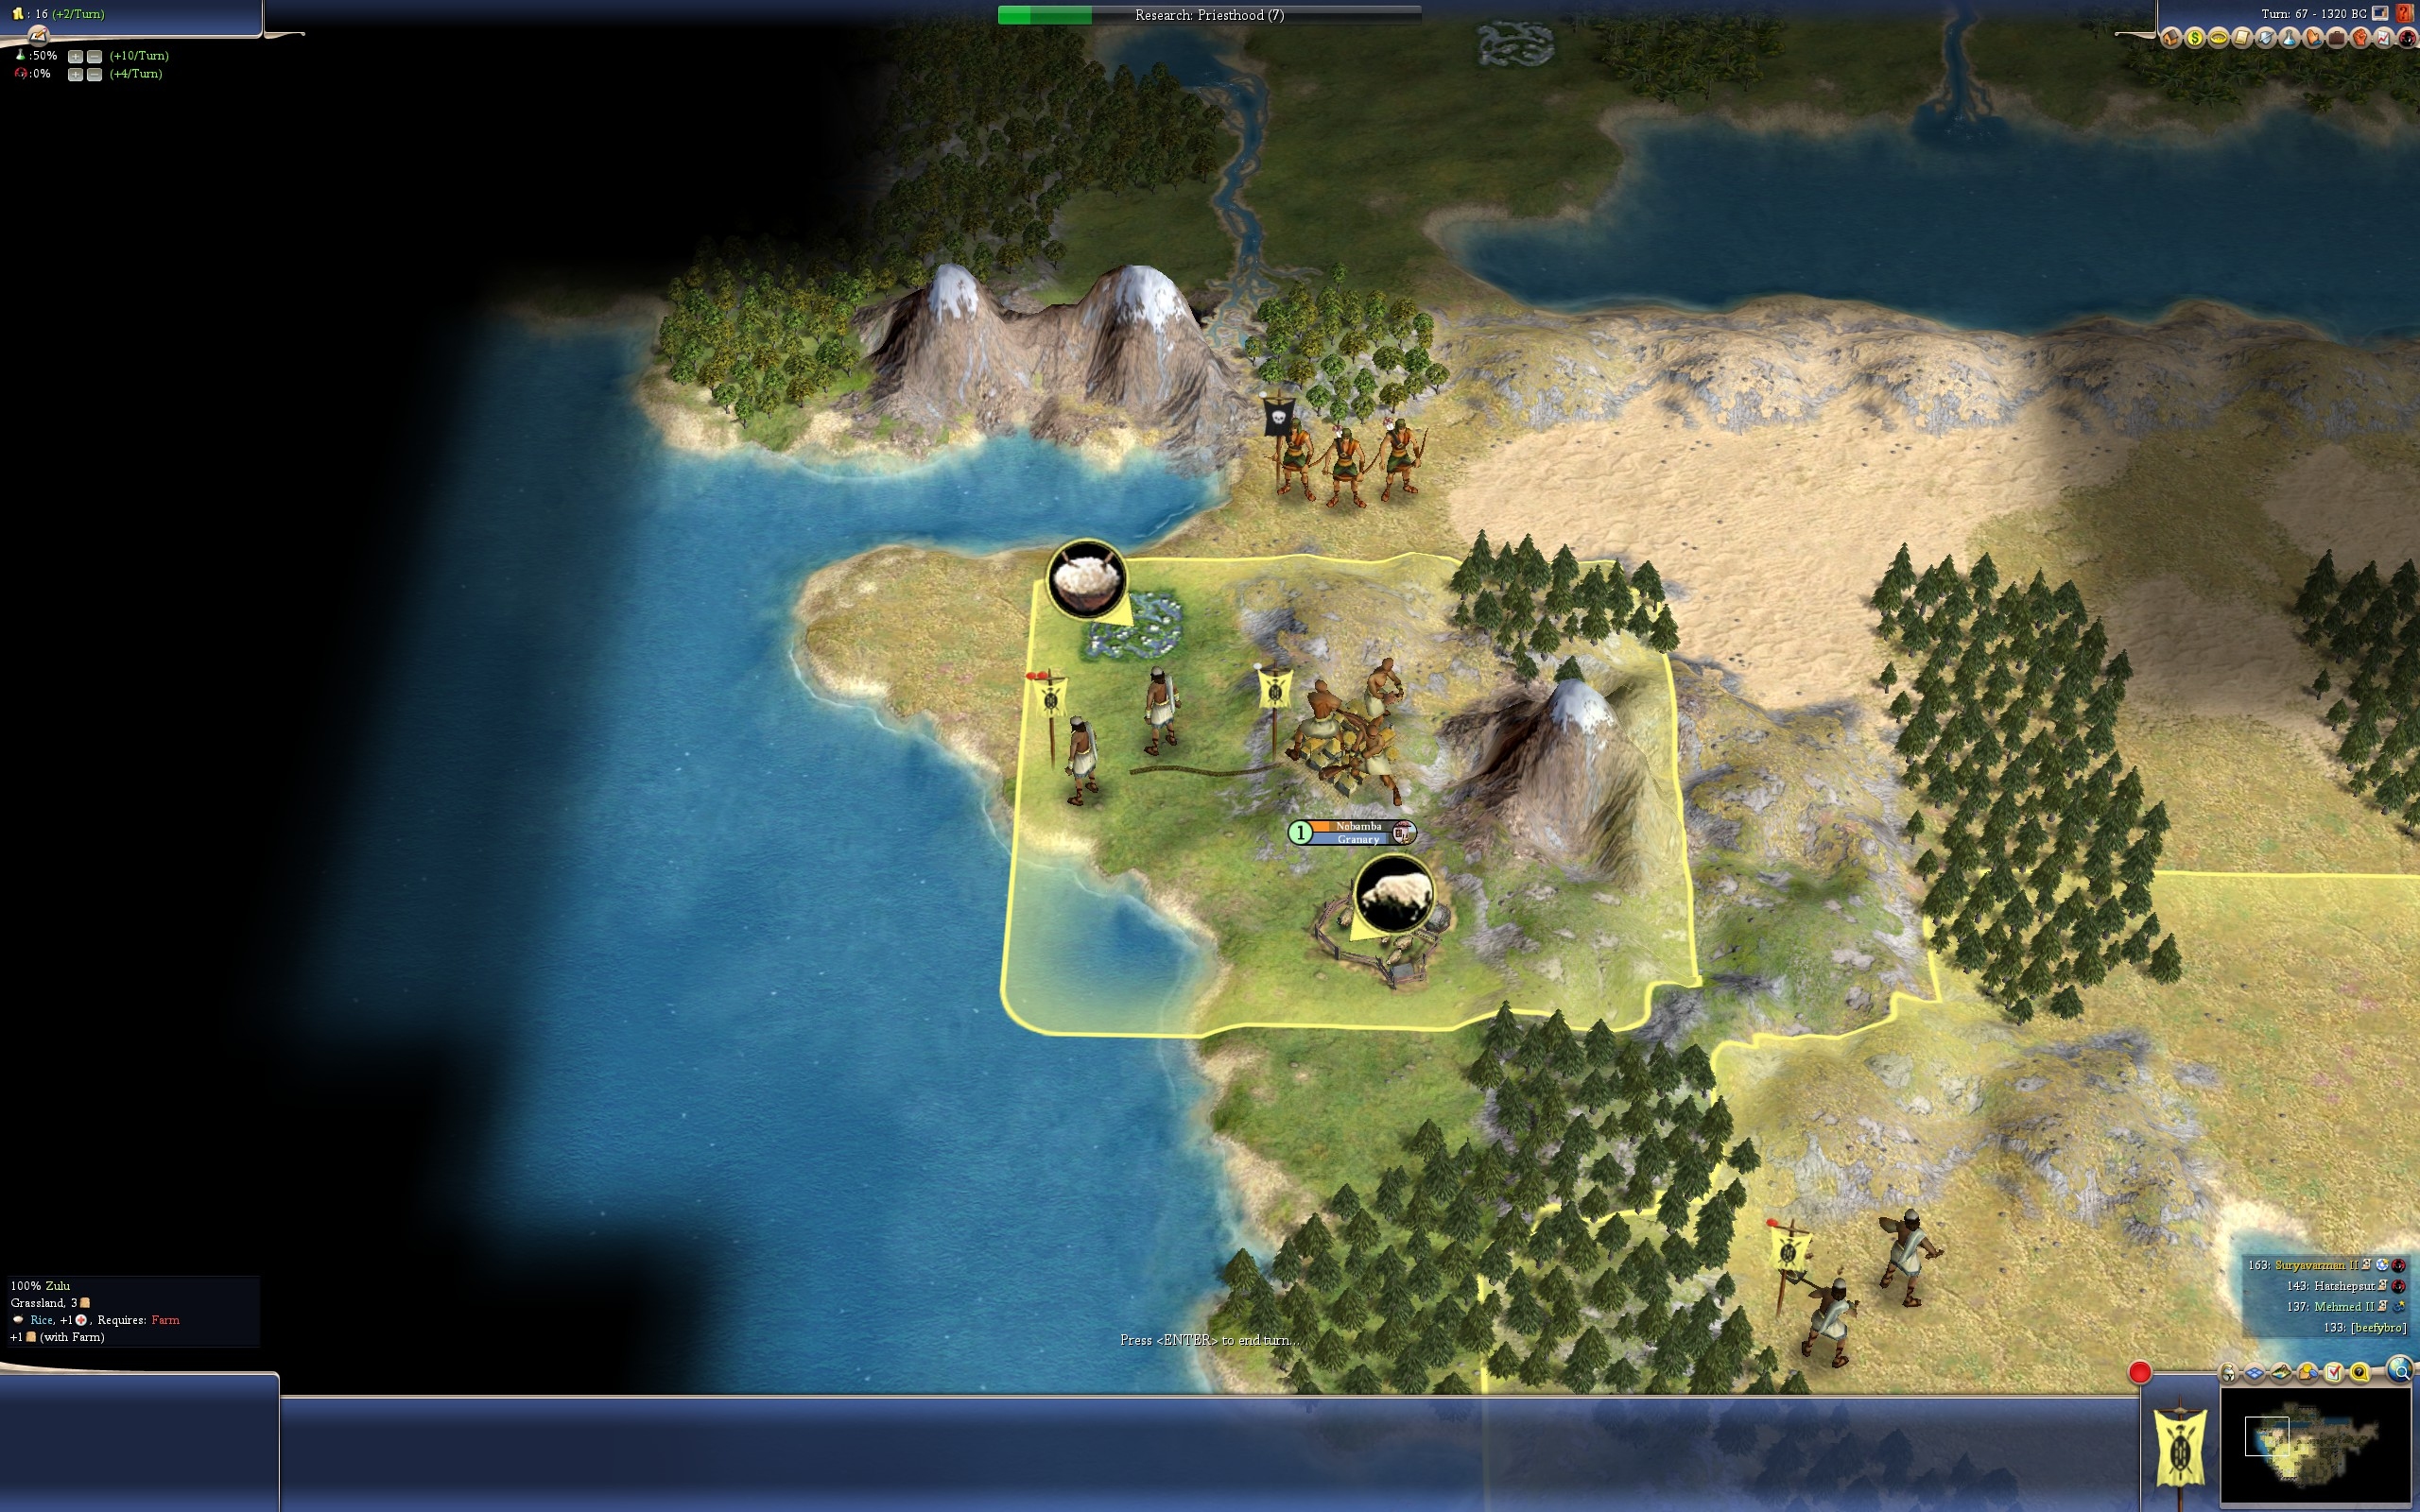
\includegraphics[width=1.0\textwidth]{34}

It's after 1500 BC (1320 BC) and on monarch difficult, non-animal
barbs are starting to spawn and attack my cities. My fortified warrior
eventually wins this fight at 75\% chance to win, but that's no way to
play an NDS game. That's basically a 1-in-4 chance of a complete
disaster for your civ. By the time these barb archers start showing
up, you MUST have either metal, horse, or archery units defending your
outer cities. I've been reckless here since this is only a demo game.

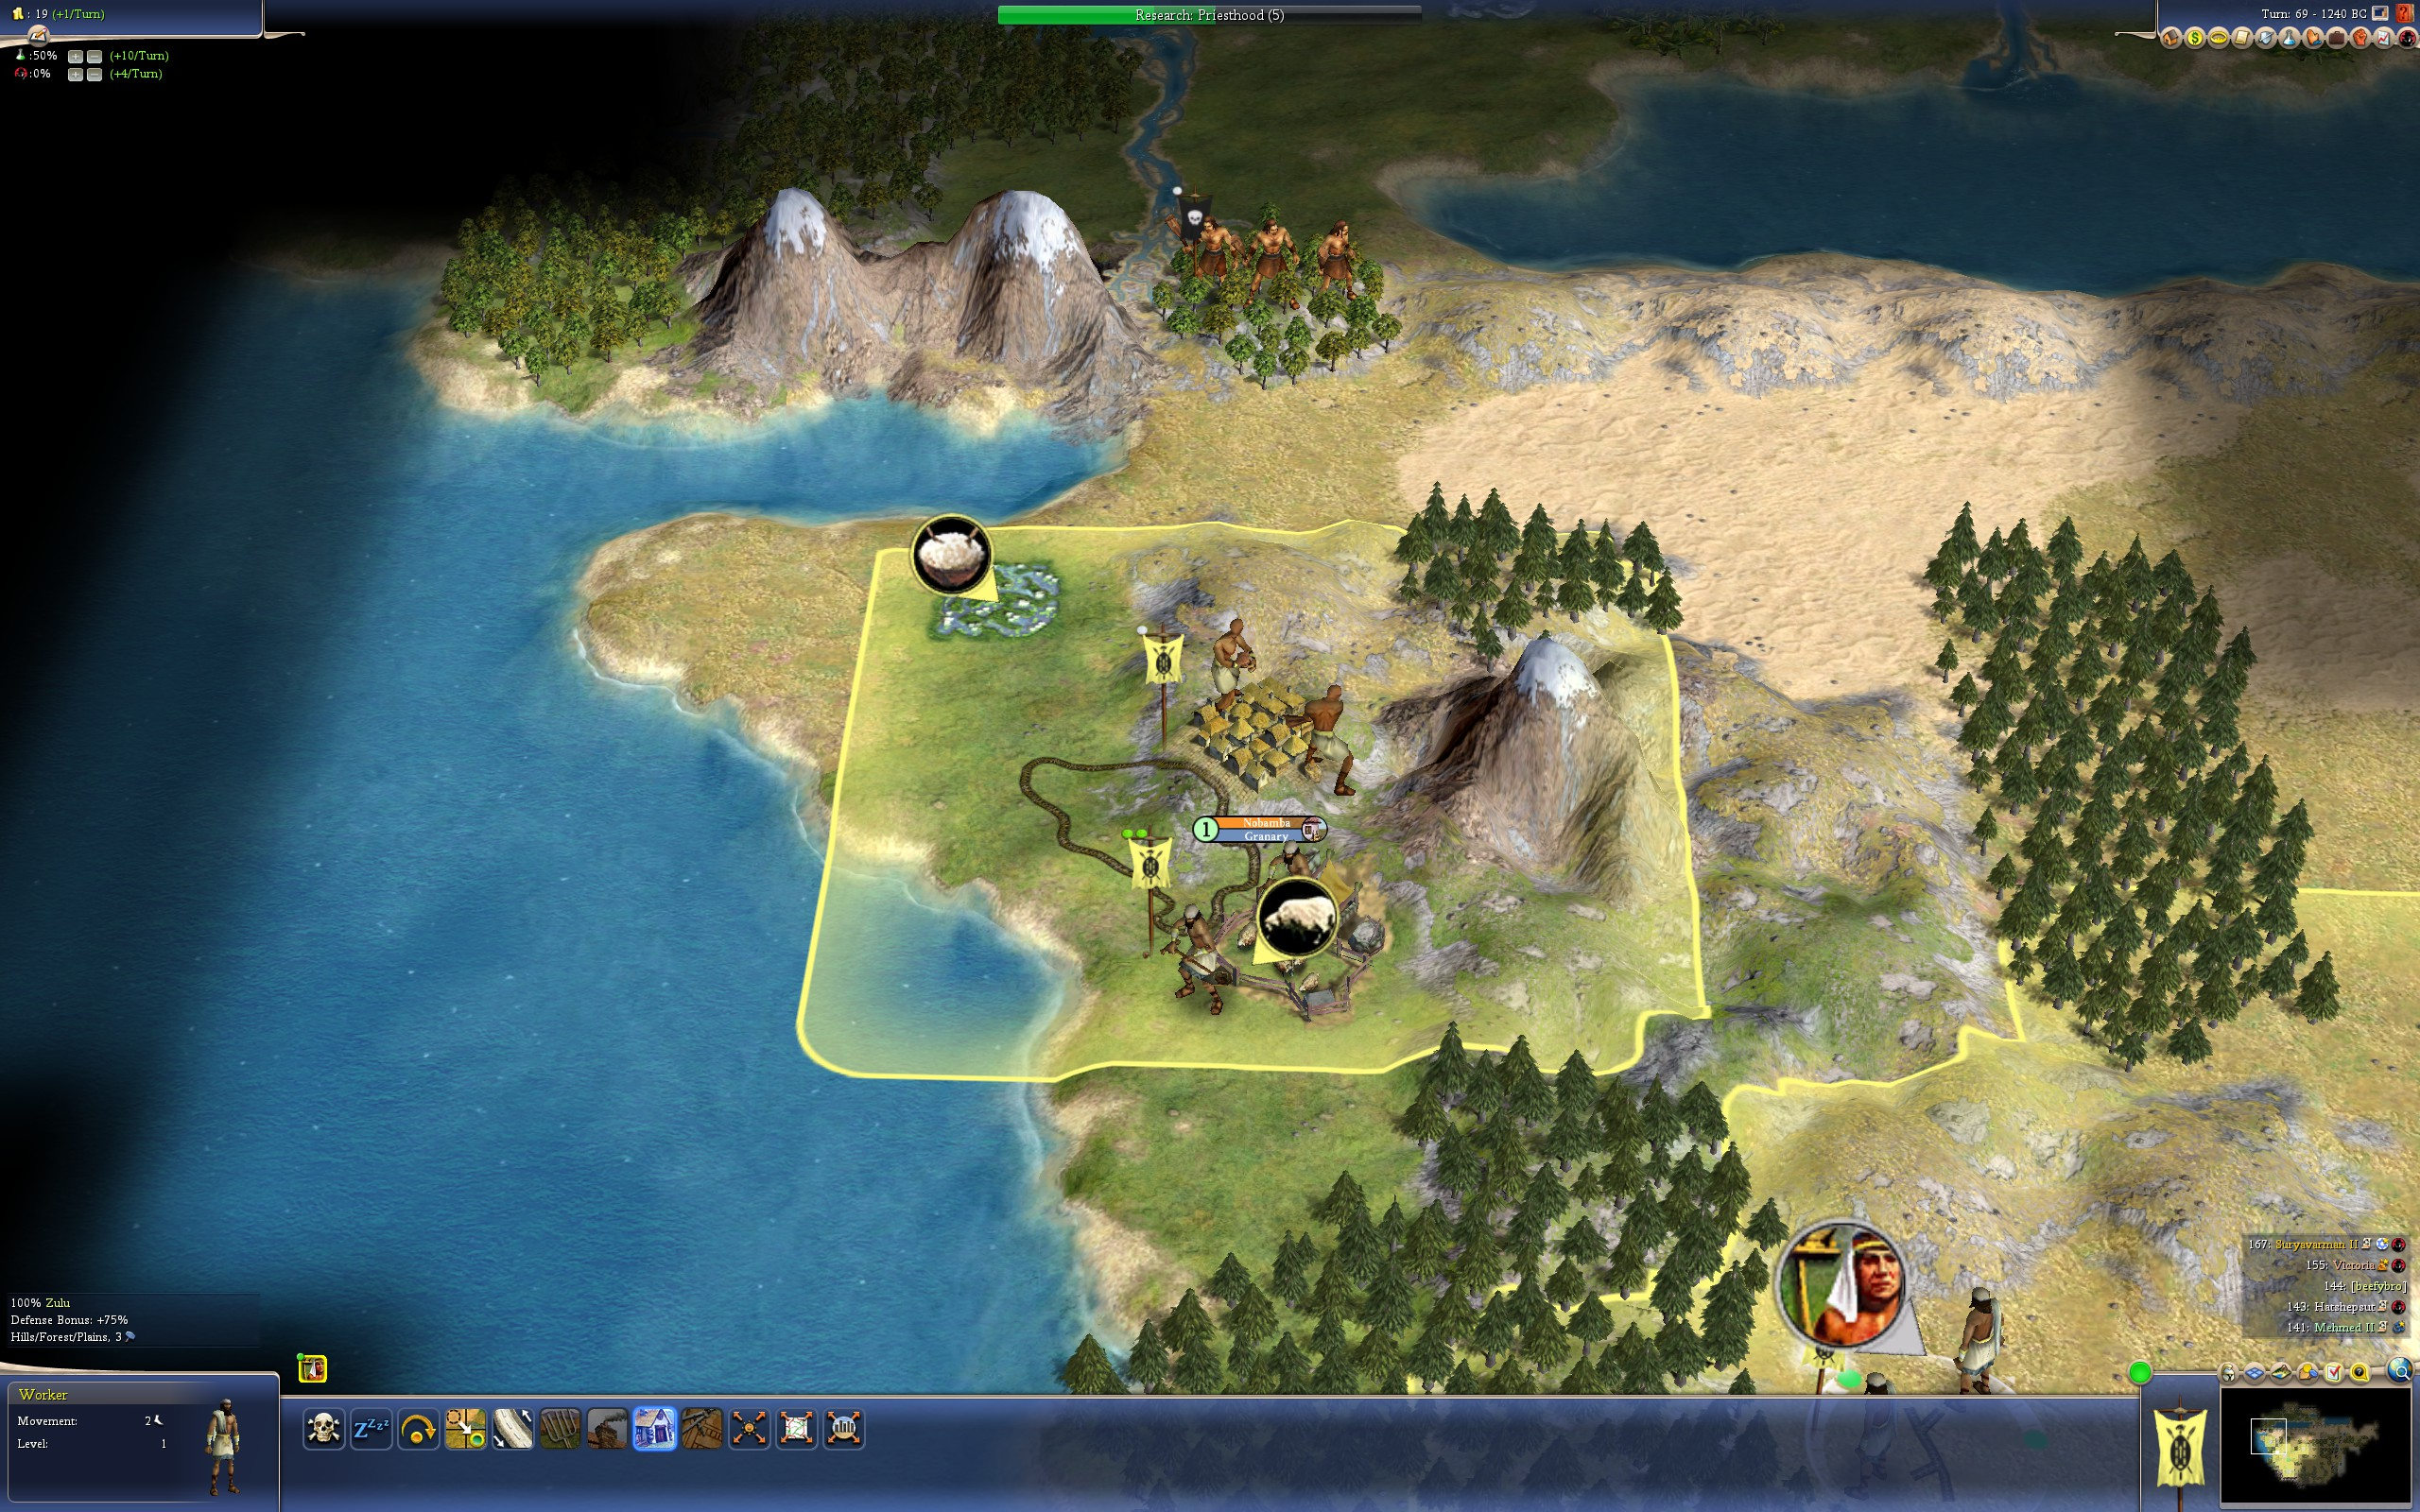
\includegraphics[width=1.0\textwidth]{36}

As more barbs come after my coastal city, I desperately build roads to try to connect this city to the
rest of my civ. This will give me a trade route and give the city access to bronze so I can build/chop
impis which should finally make this city safe.

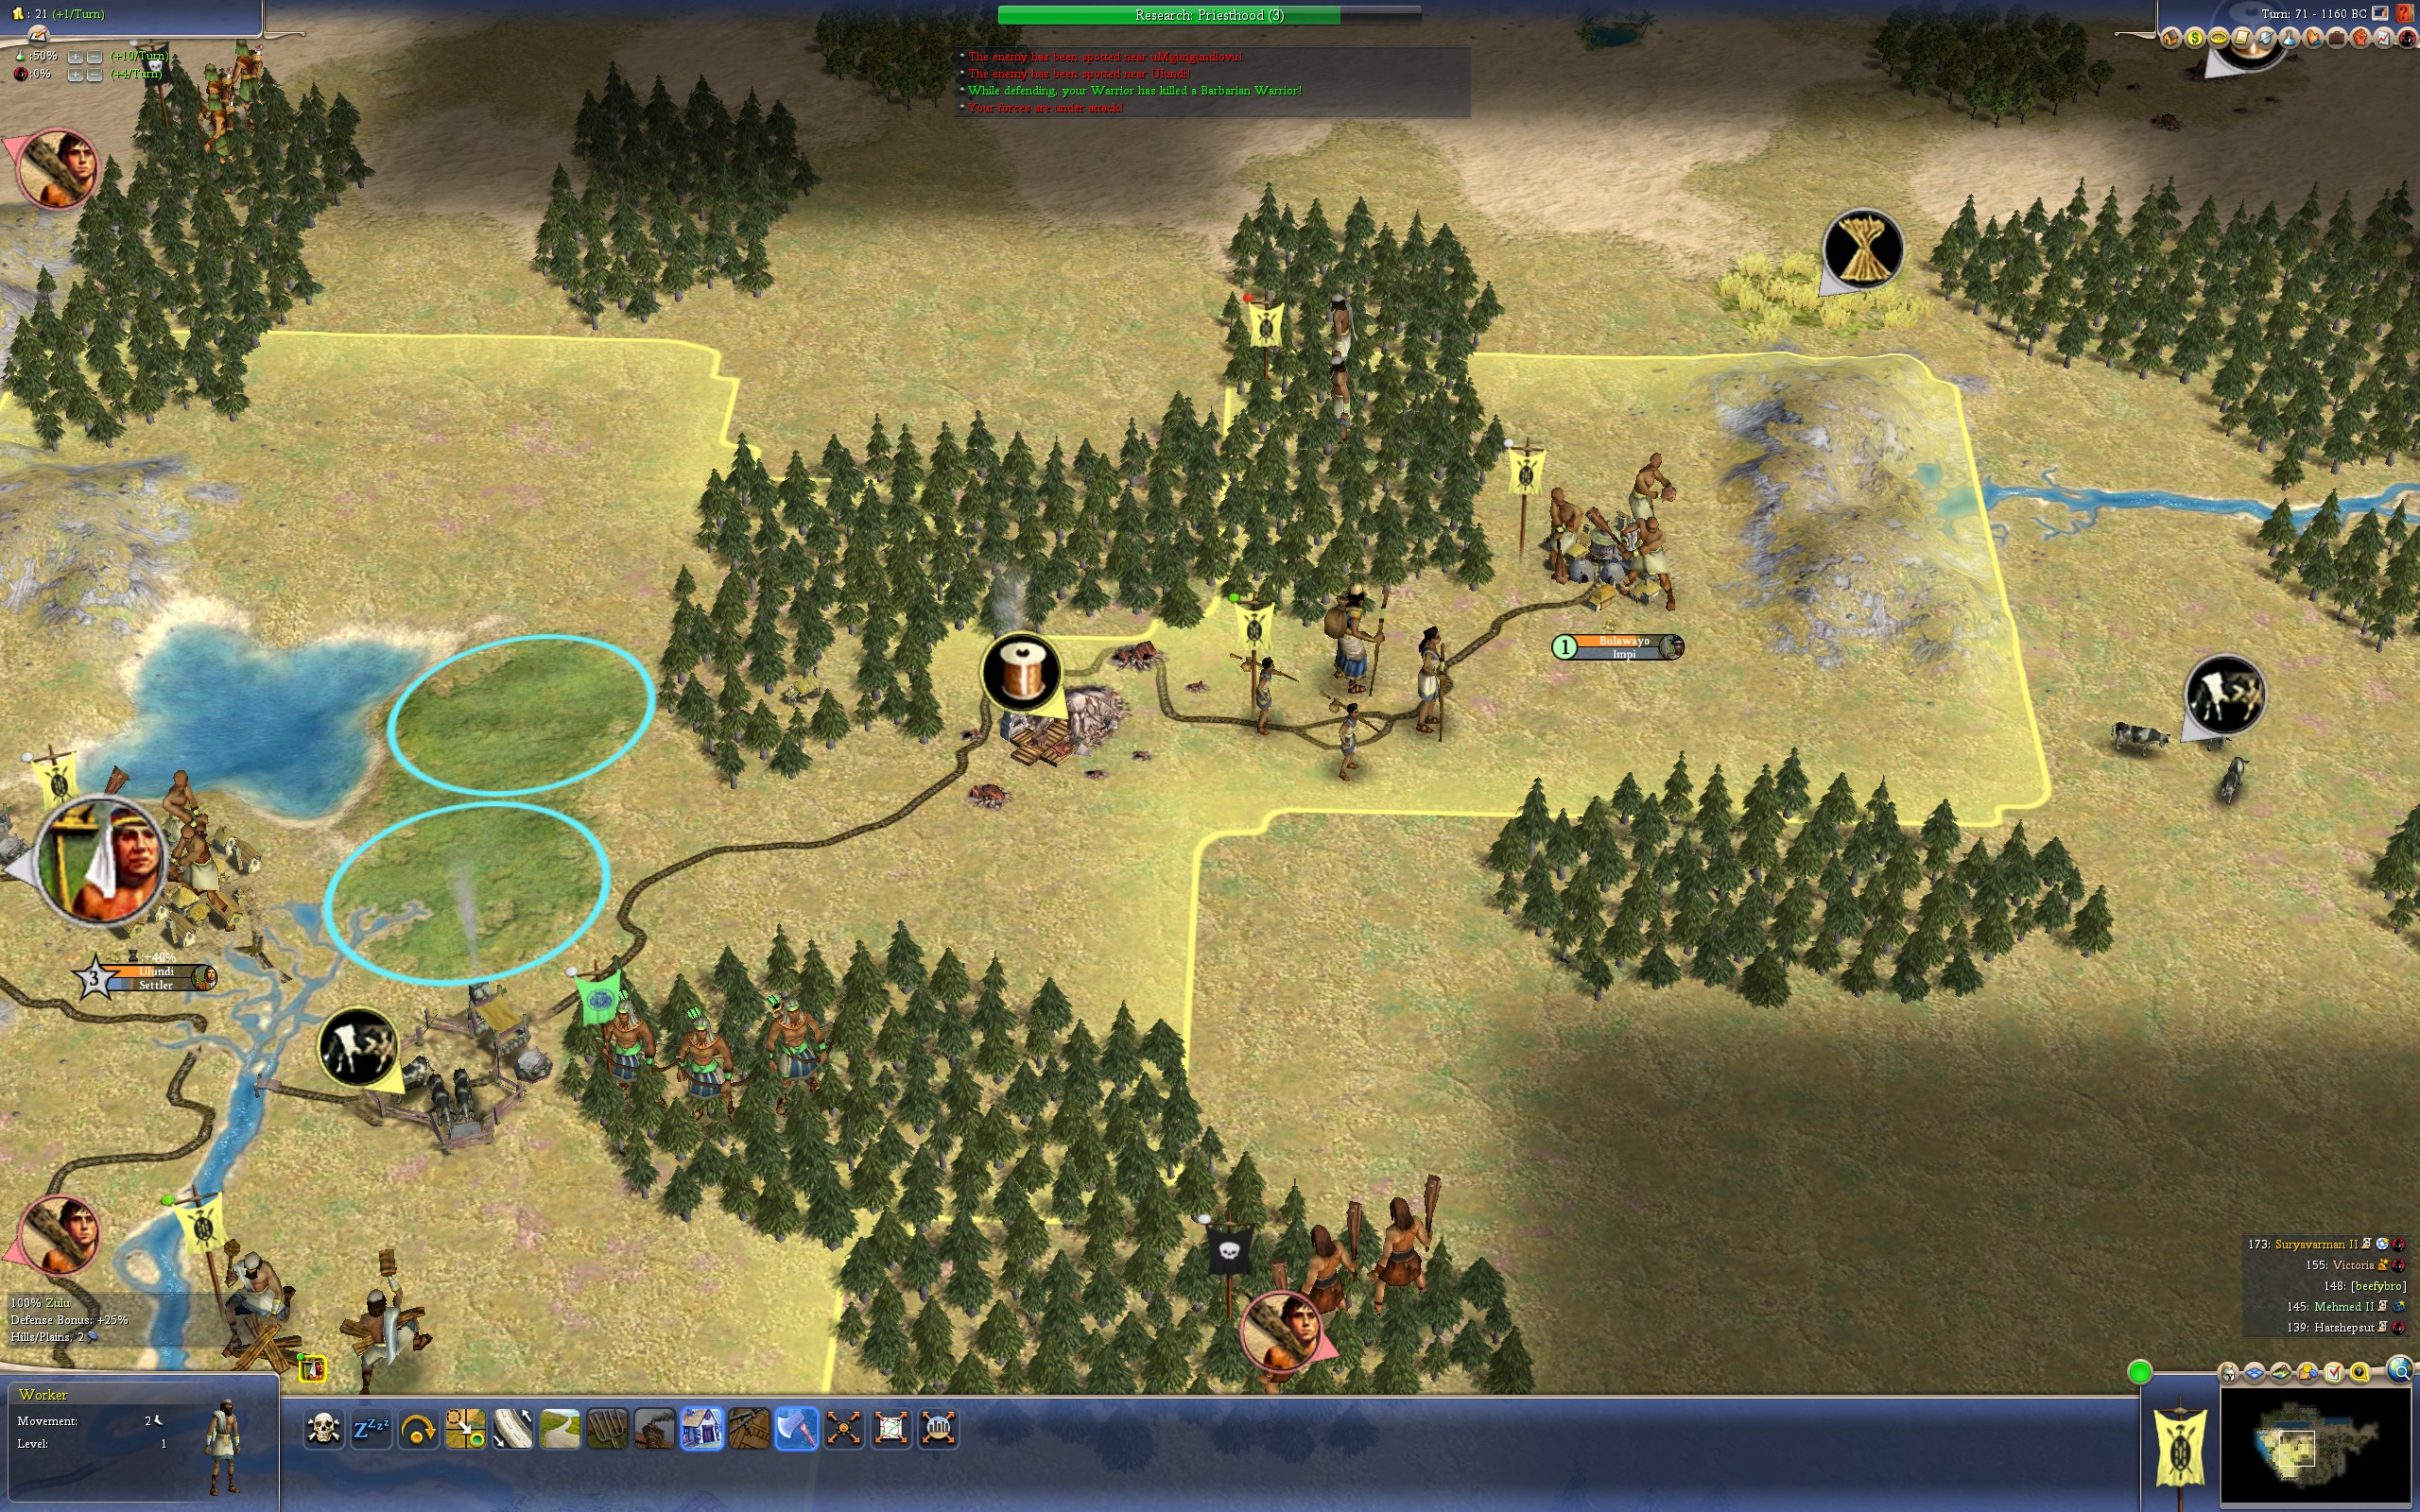
\includegraphics[width=1.0\textwidth]{37}

Just showing the action. Settler racing east to claim land before Hatty gets there. Barbs continue to spawn
all over. Impis are desperately chopped in my military city.

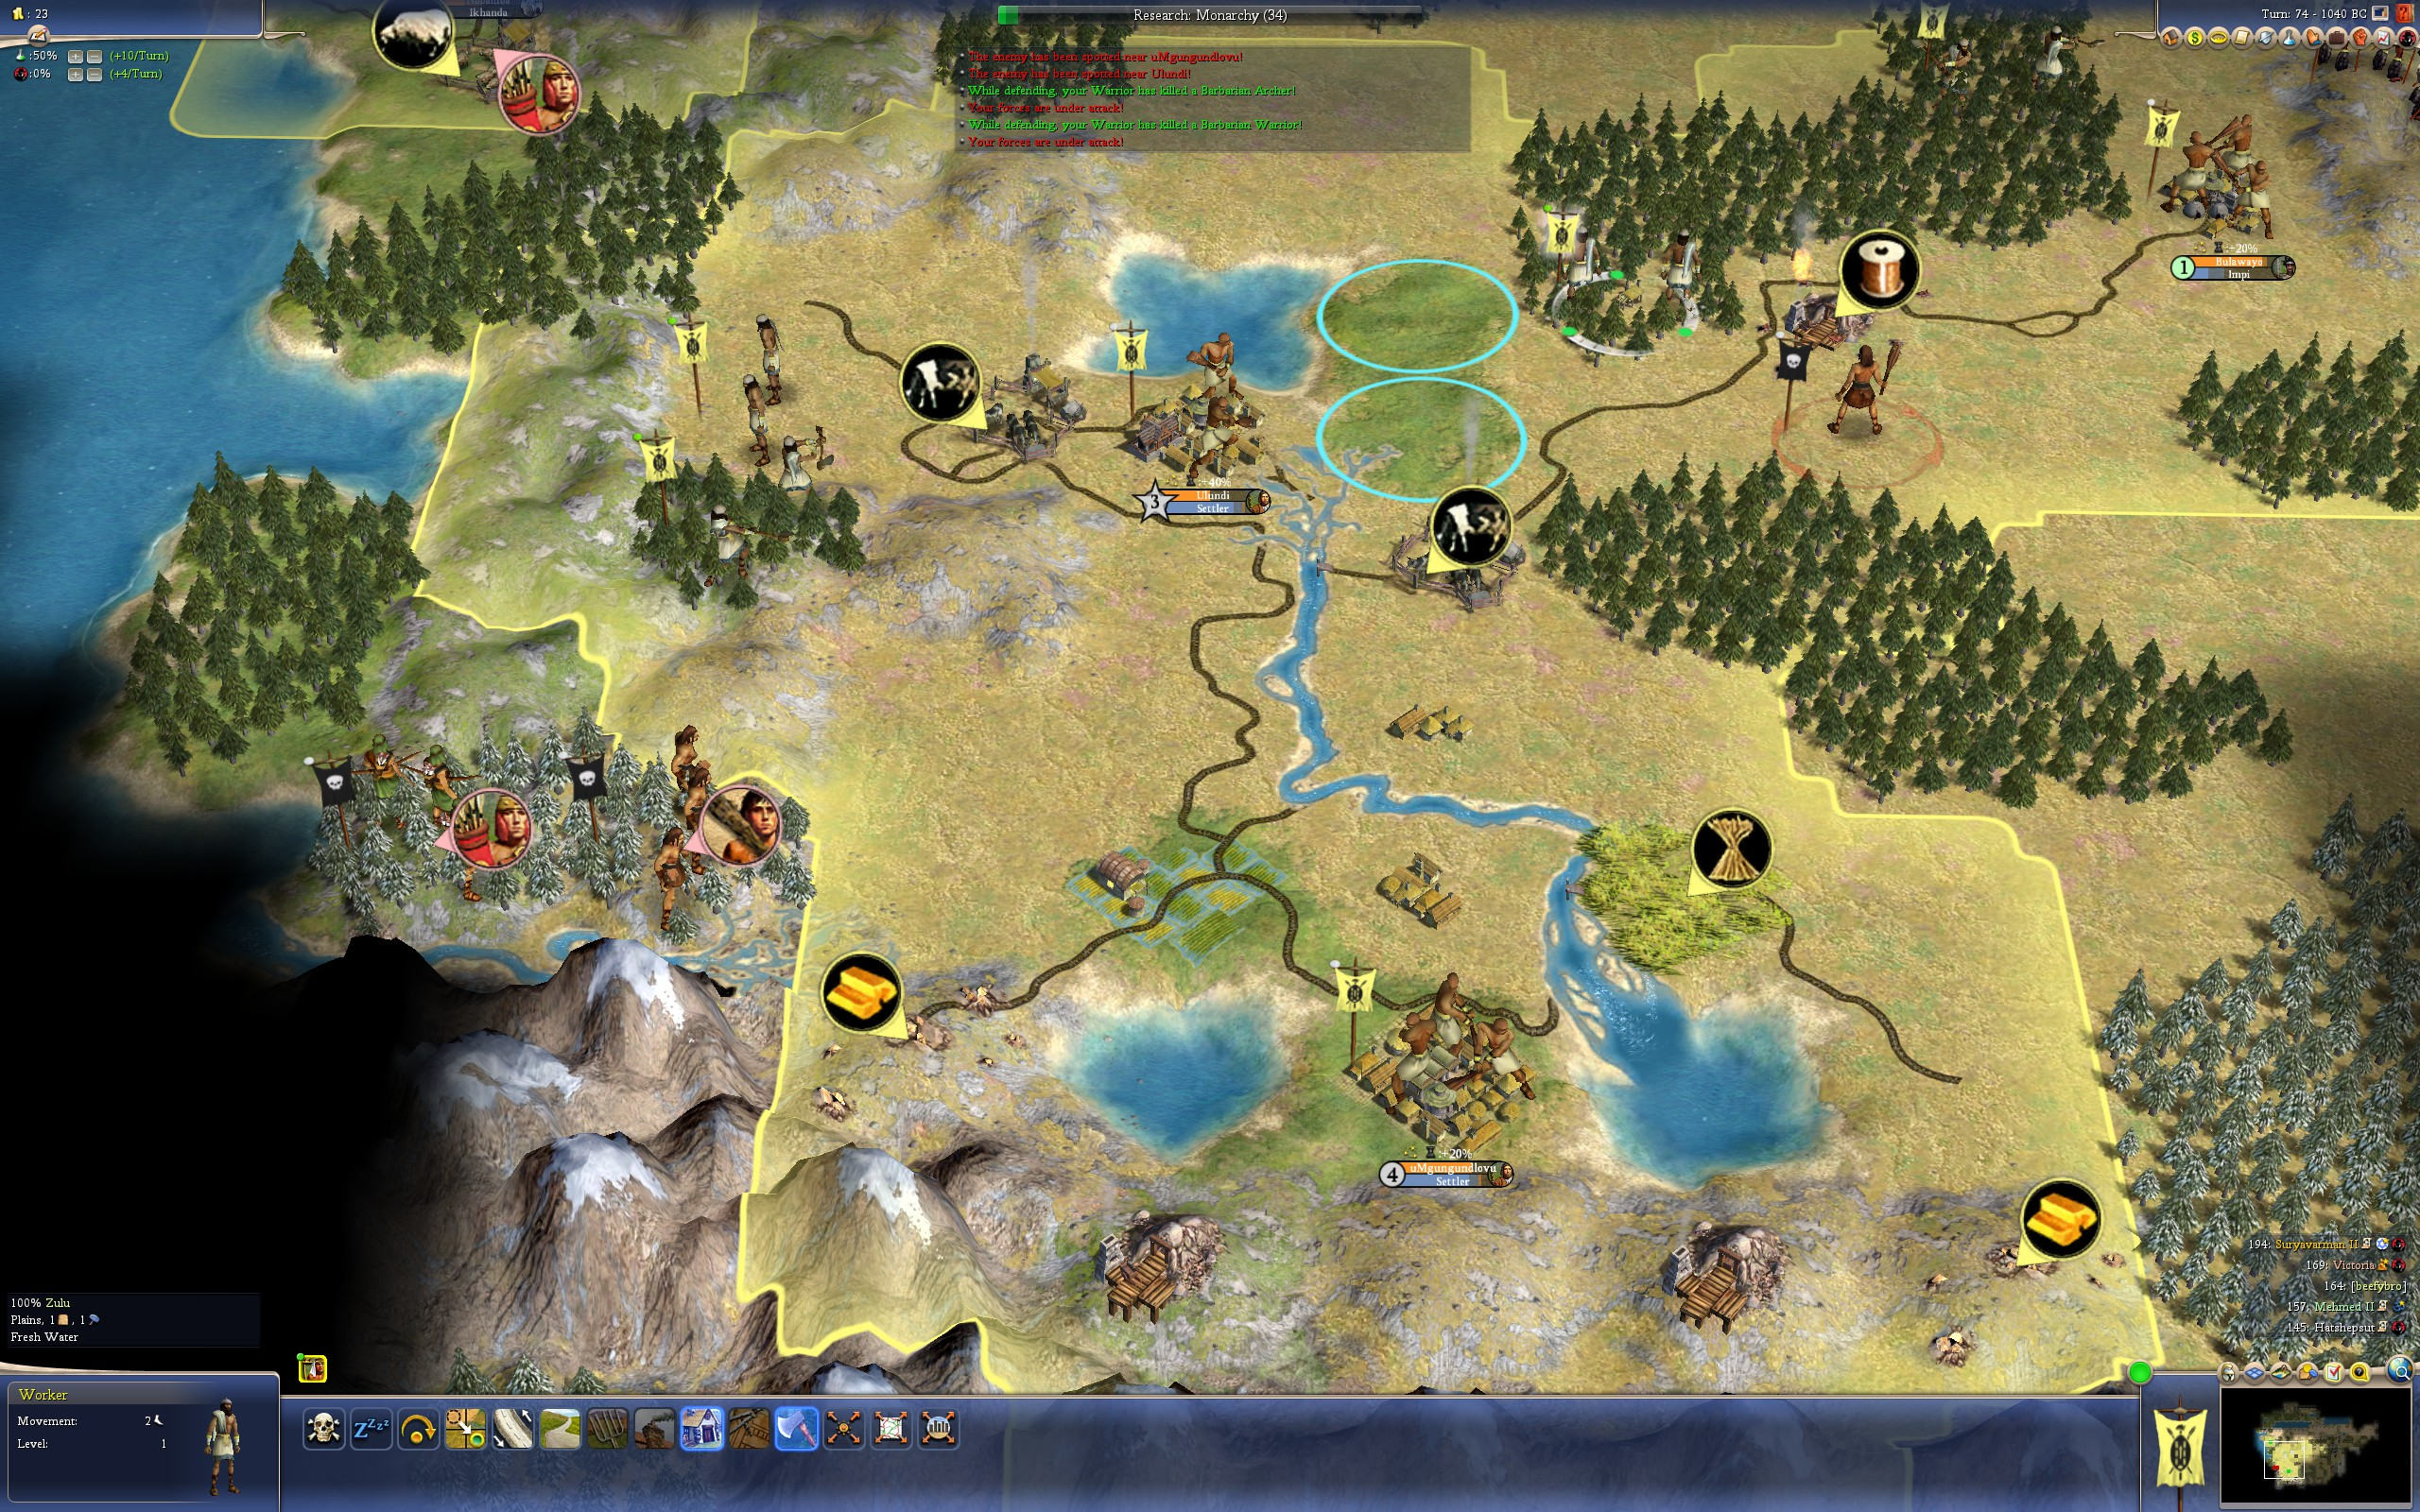
\includegraphics[width=1.0\textwidth]{39}

Barbs everywhere! Tectonic lakes is known for this, don't be caught unaware. It's still before 1000 BC.

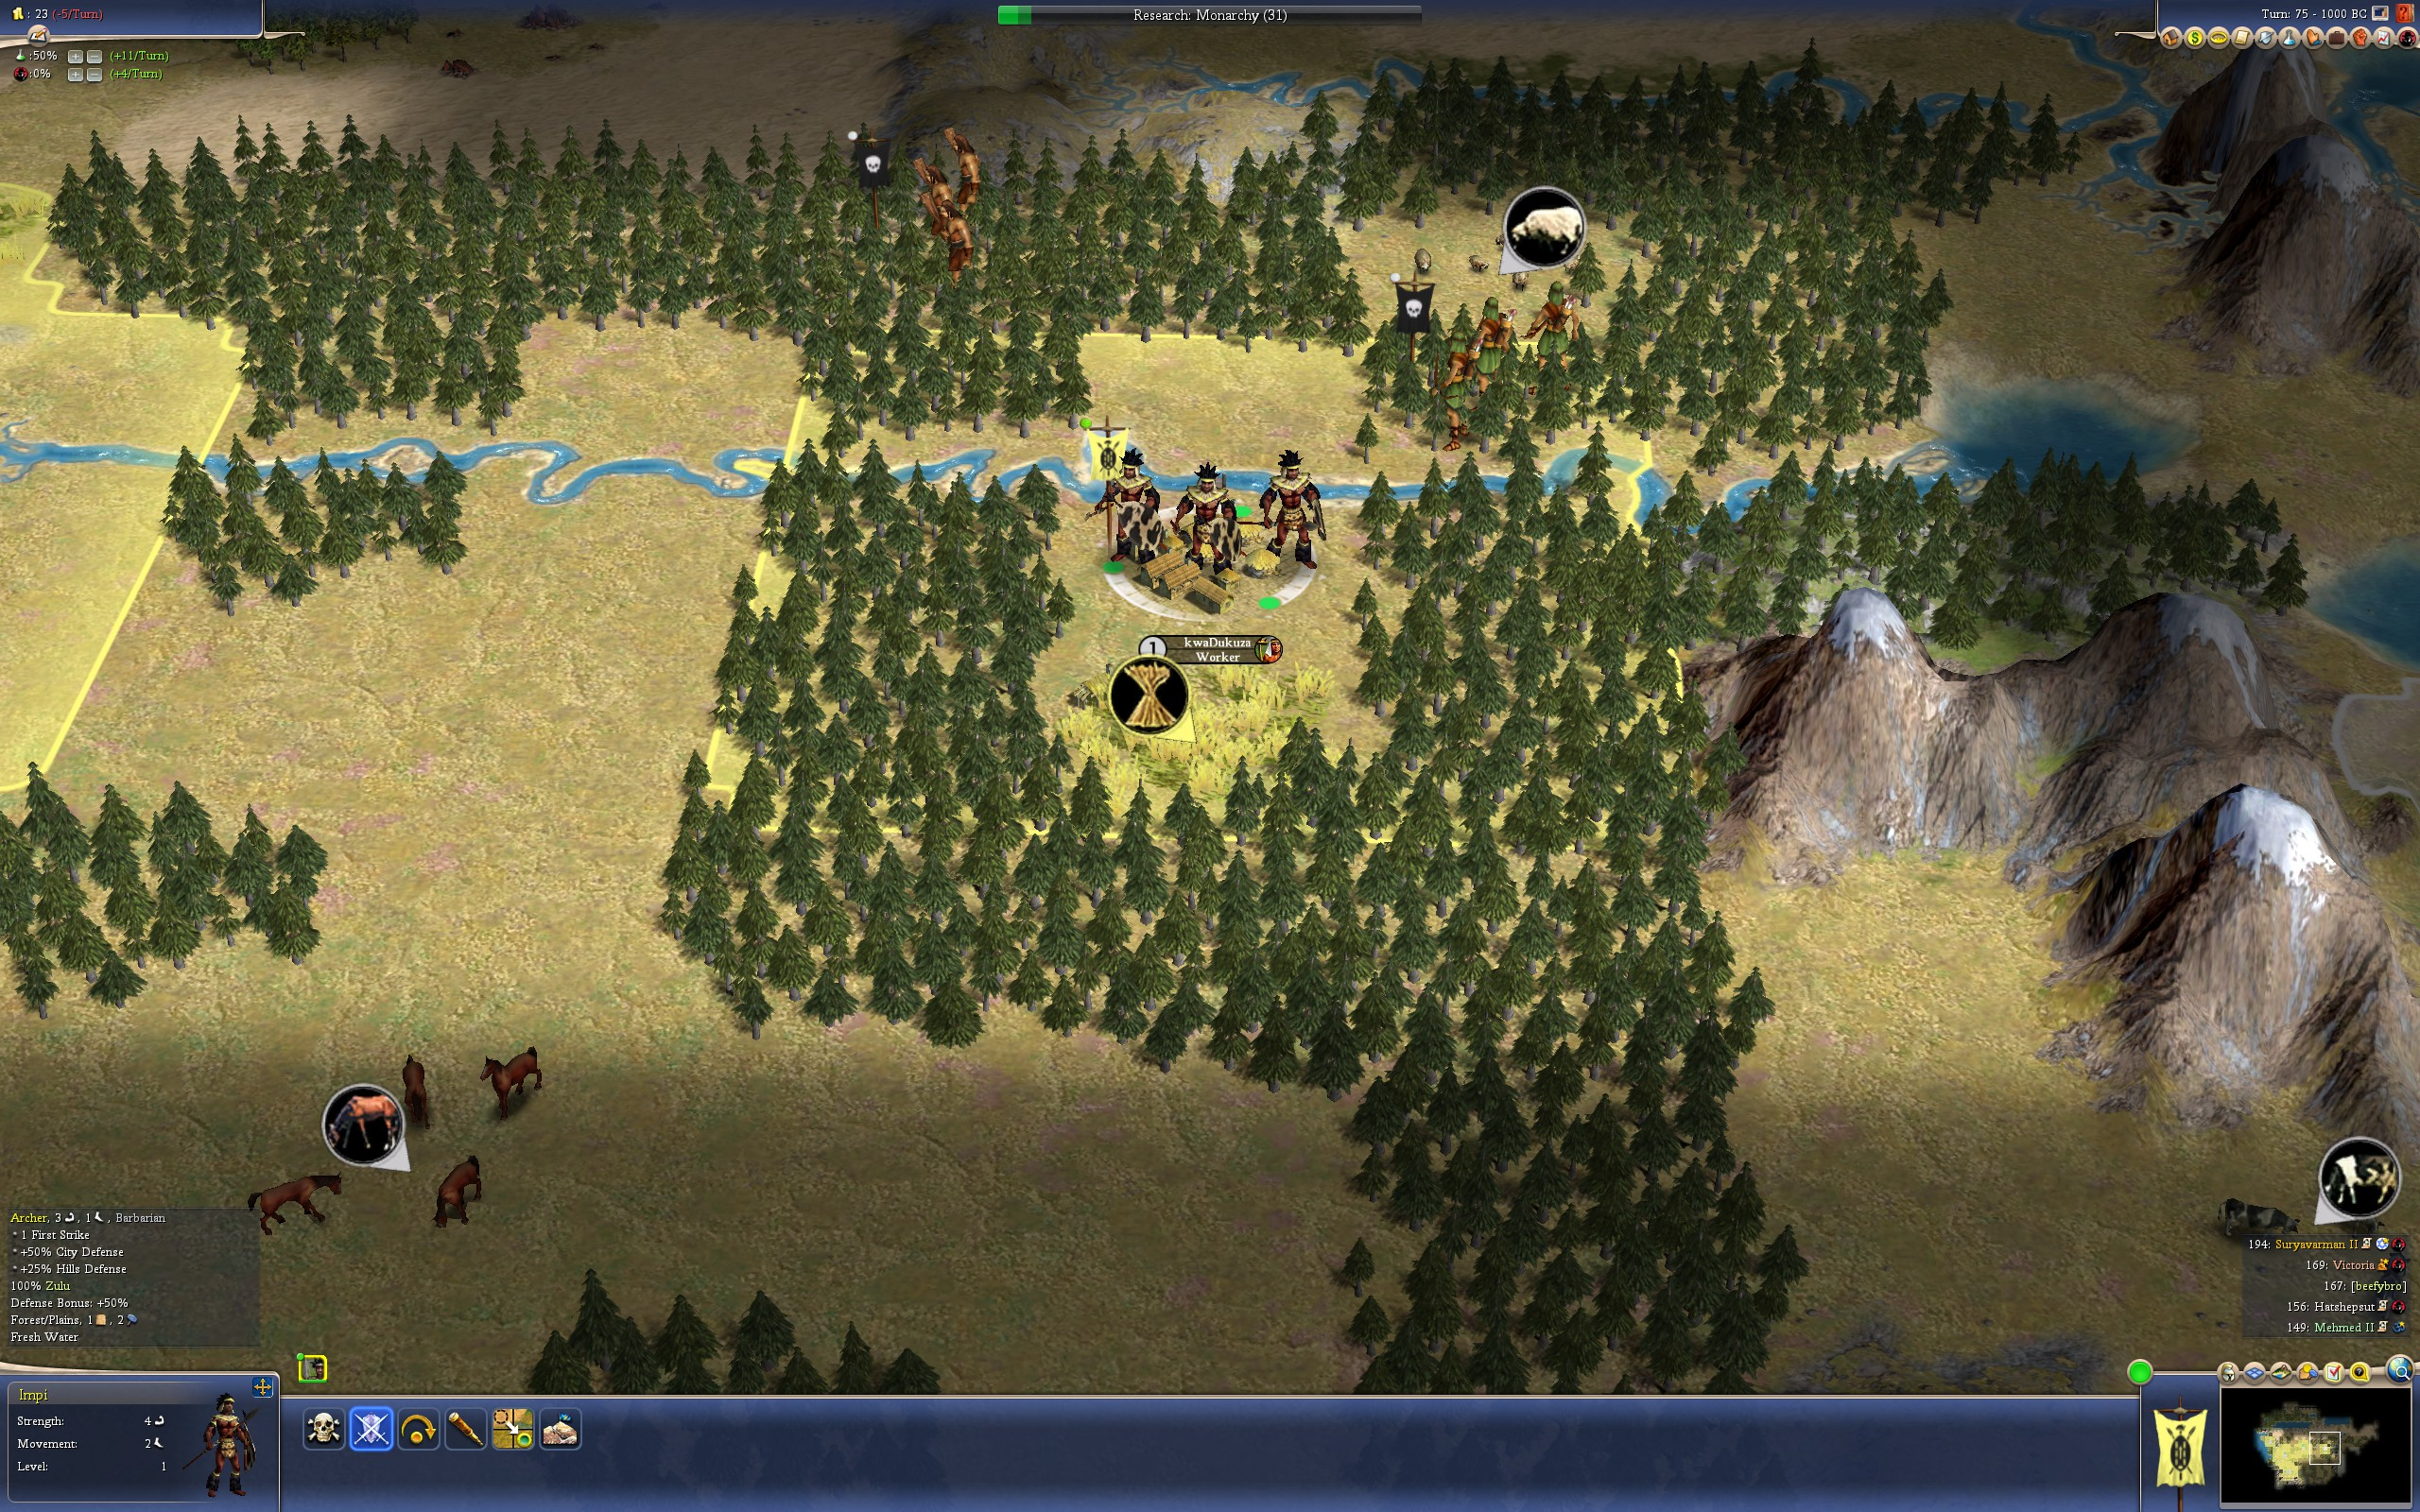
\includegraphics[width=1.0\textwidth]{42}

Success! A far-east city to claim all the best riverland from Hatty is established with the help of
an impi. With this many barbs around, a warrior or archer escort would have been too risky. Also, notice
that my economy is starting to take a beating. I've made a lot of cities (5) for 1000 BC and this one is
pretty far from my capital, so city maintenance is starting to really bite.

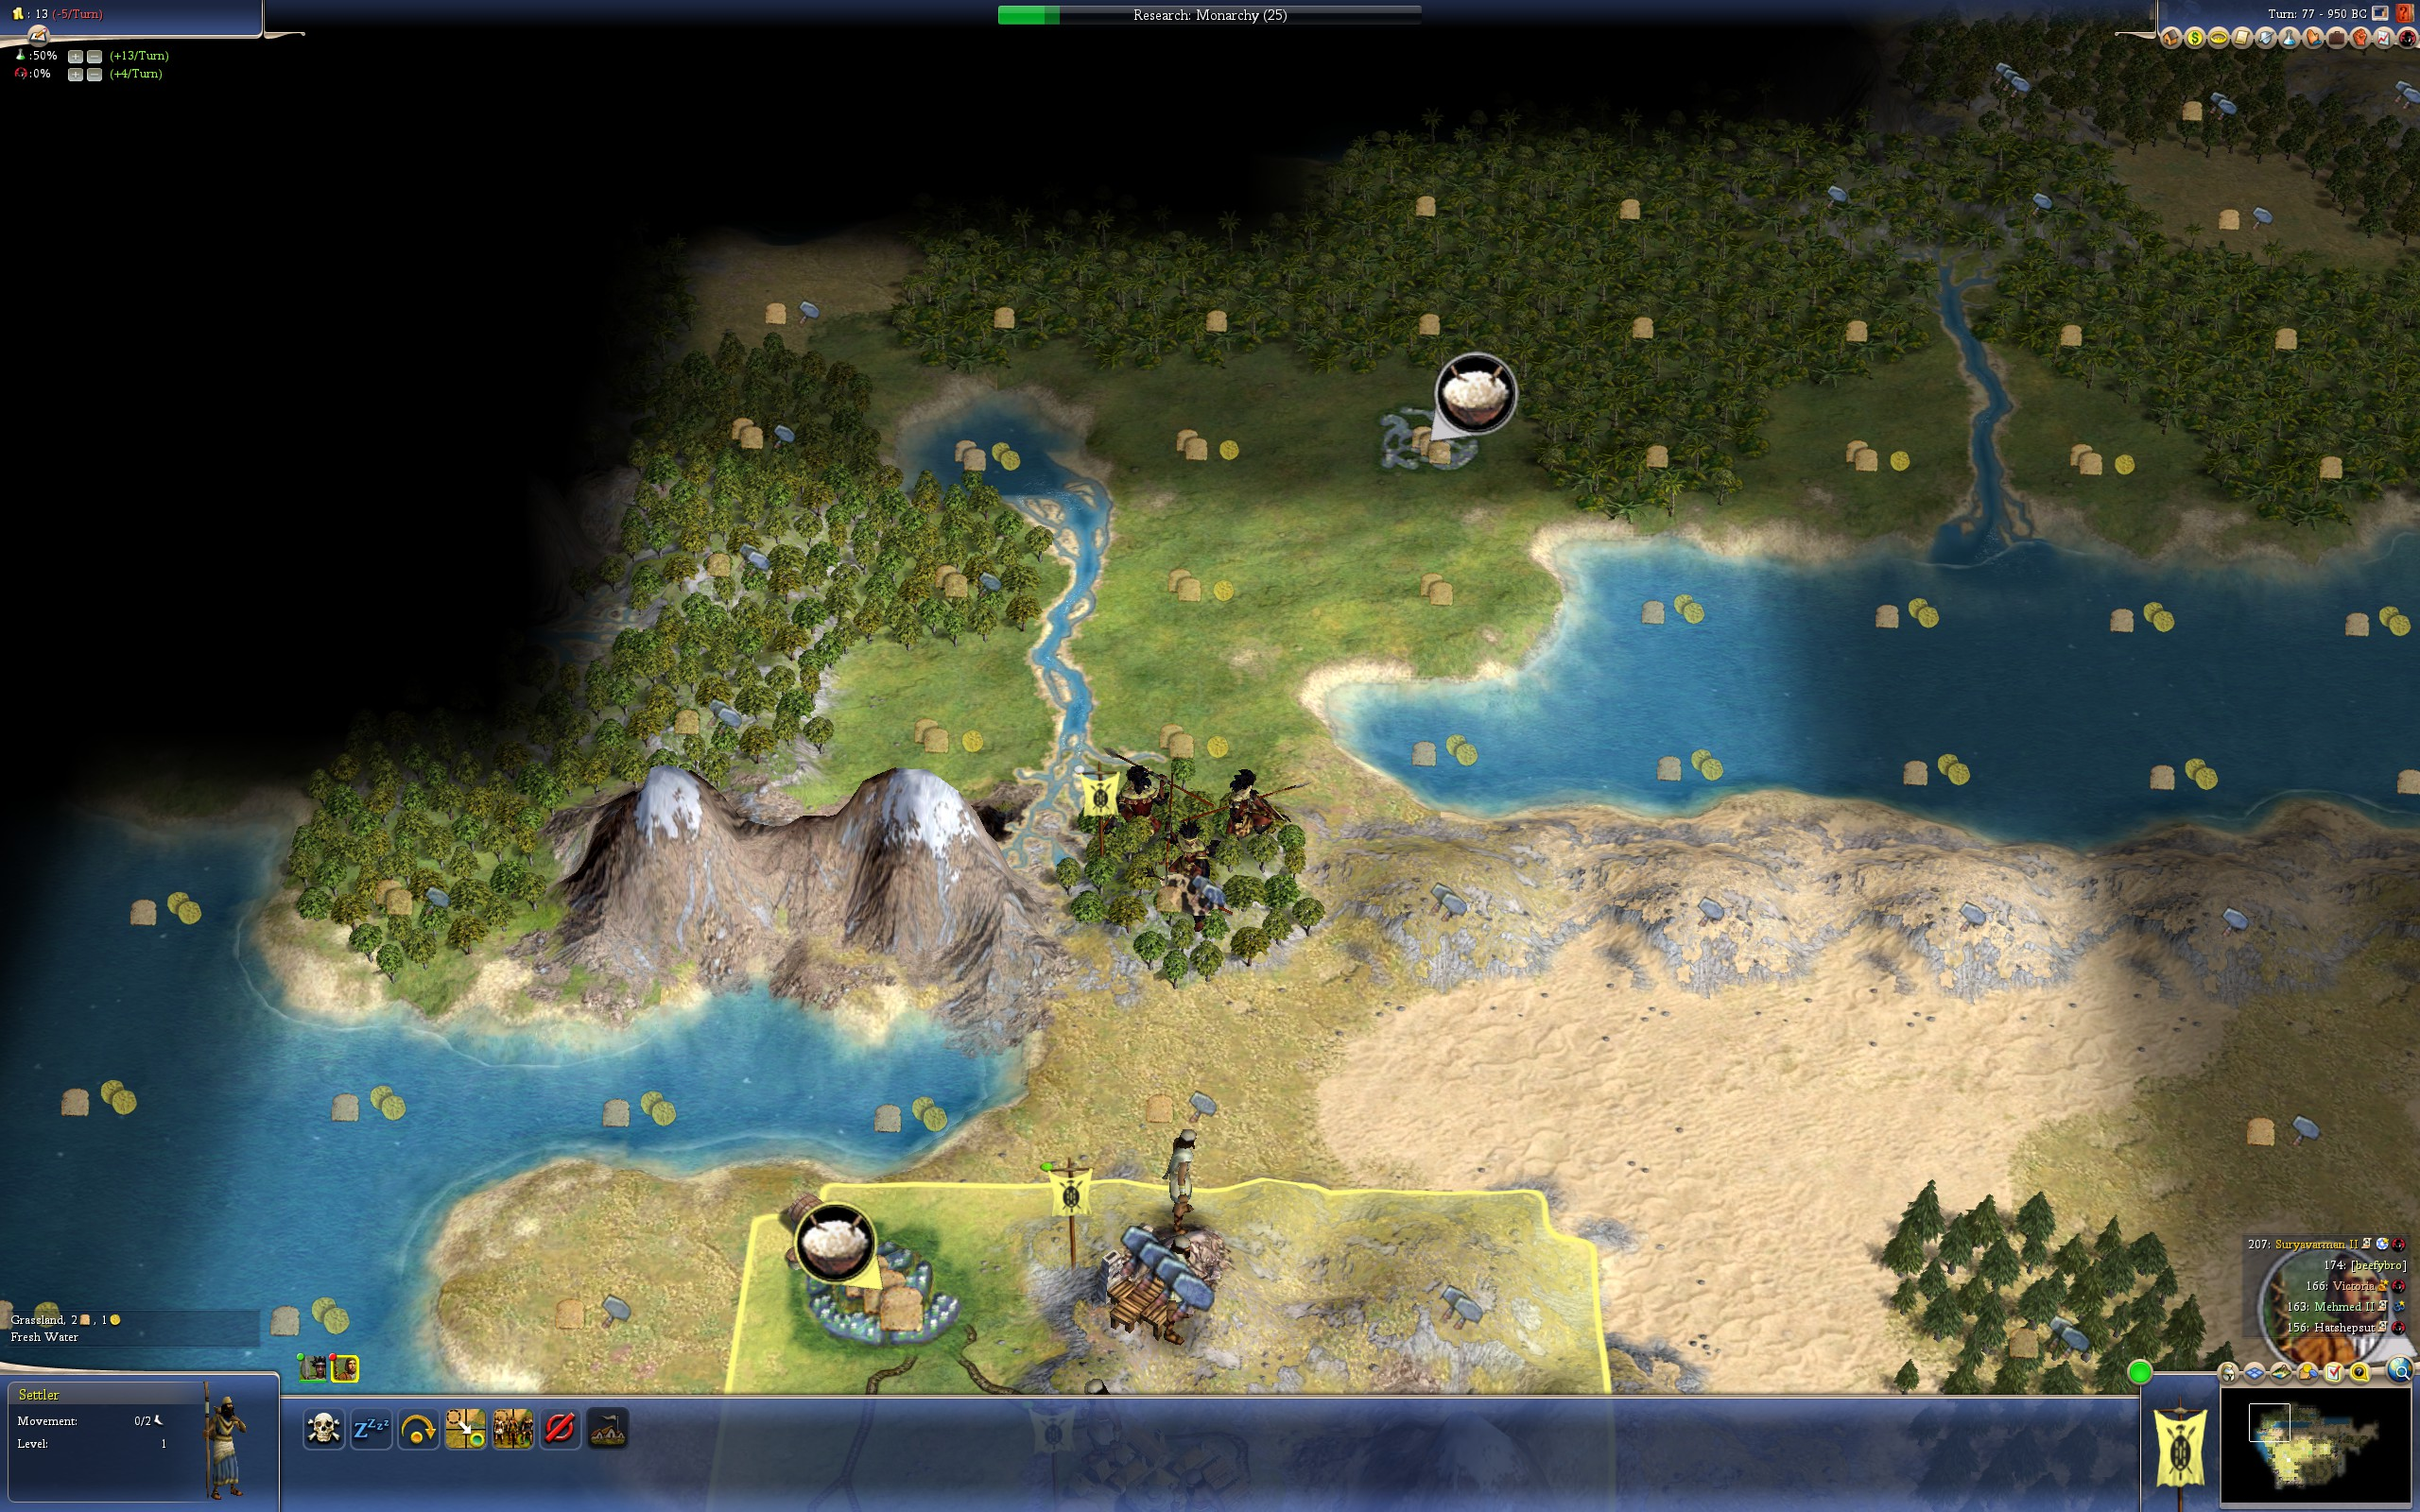
\includegraphics[width=1.0\textwidth]{43}

Some very good land to my north. I really love green tiles. They make it so much easier for your city
to grow without having to have massive food surplus tiles. I will start settling here soon once I'm sure
Hatty won't get any of the land to the east that I want.

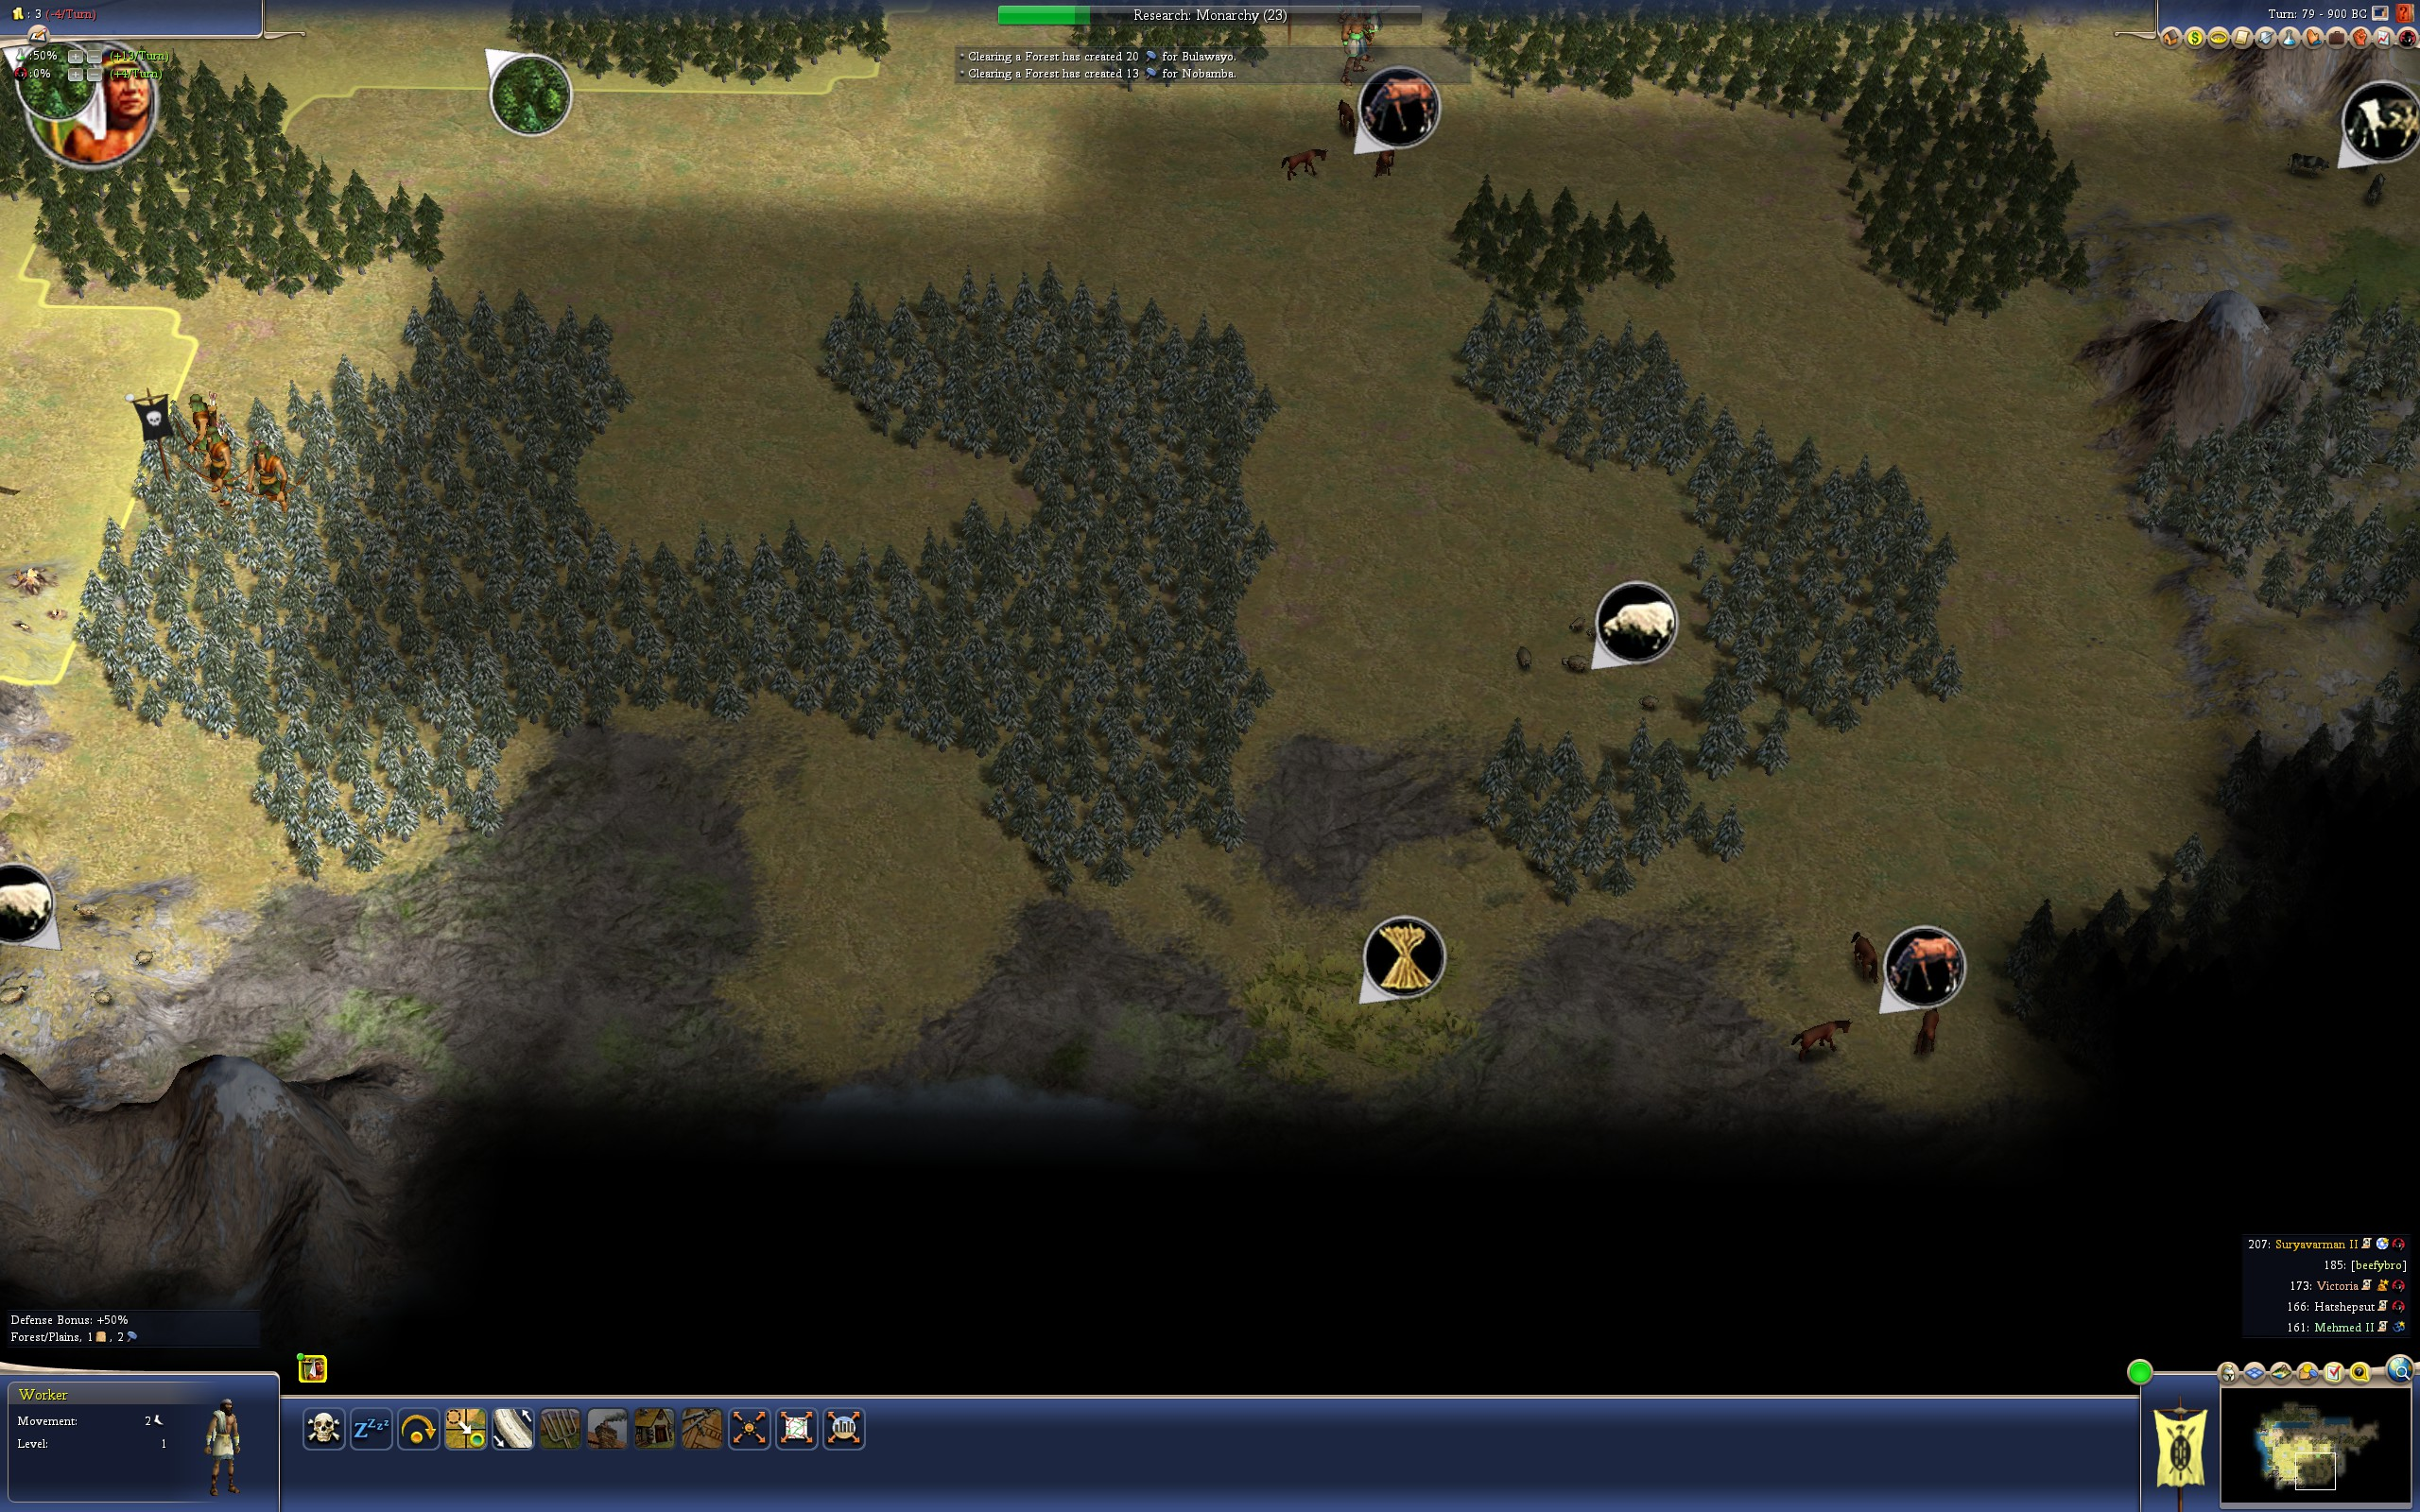
\includegraphics[width=1.0\textwidth]{46}

Speaking of east land, I see a spot that picks up sheep, wheat, and horse. I want to get here before
Hatty does. As with most of my land, brown tiles are an issue, but having three bonus resources in
one city is almost always a good thing.

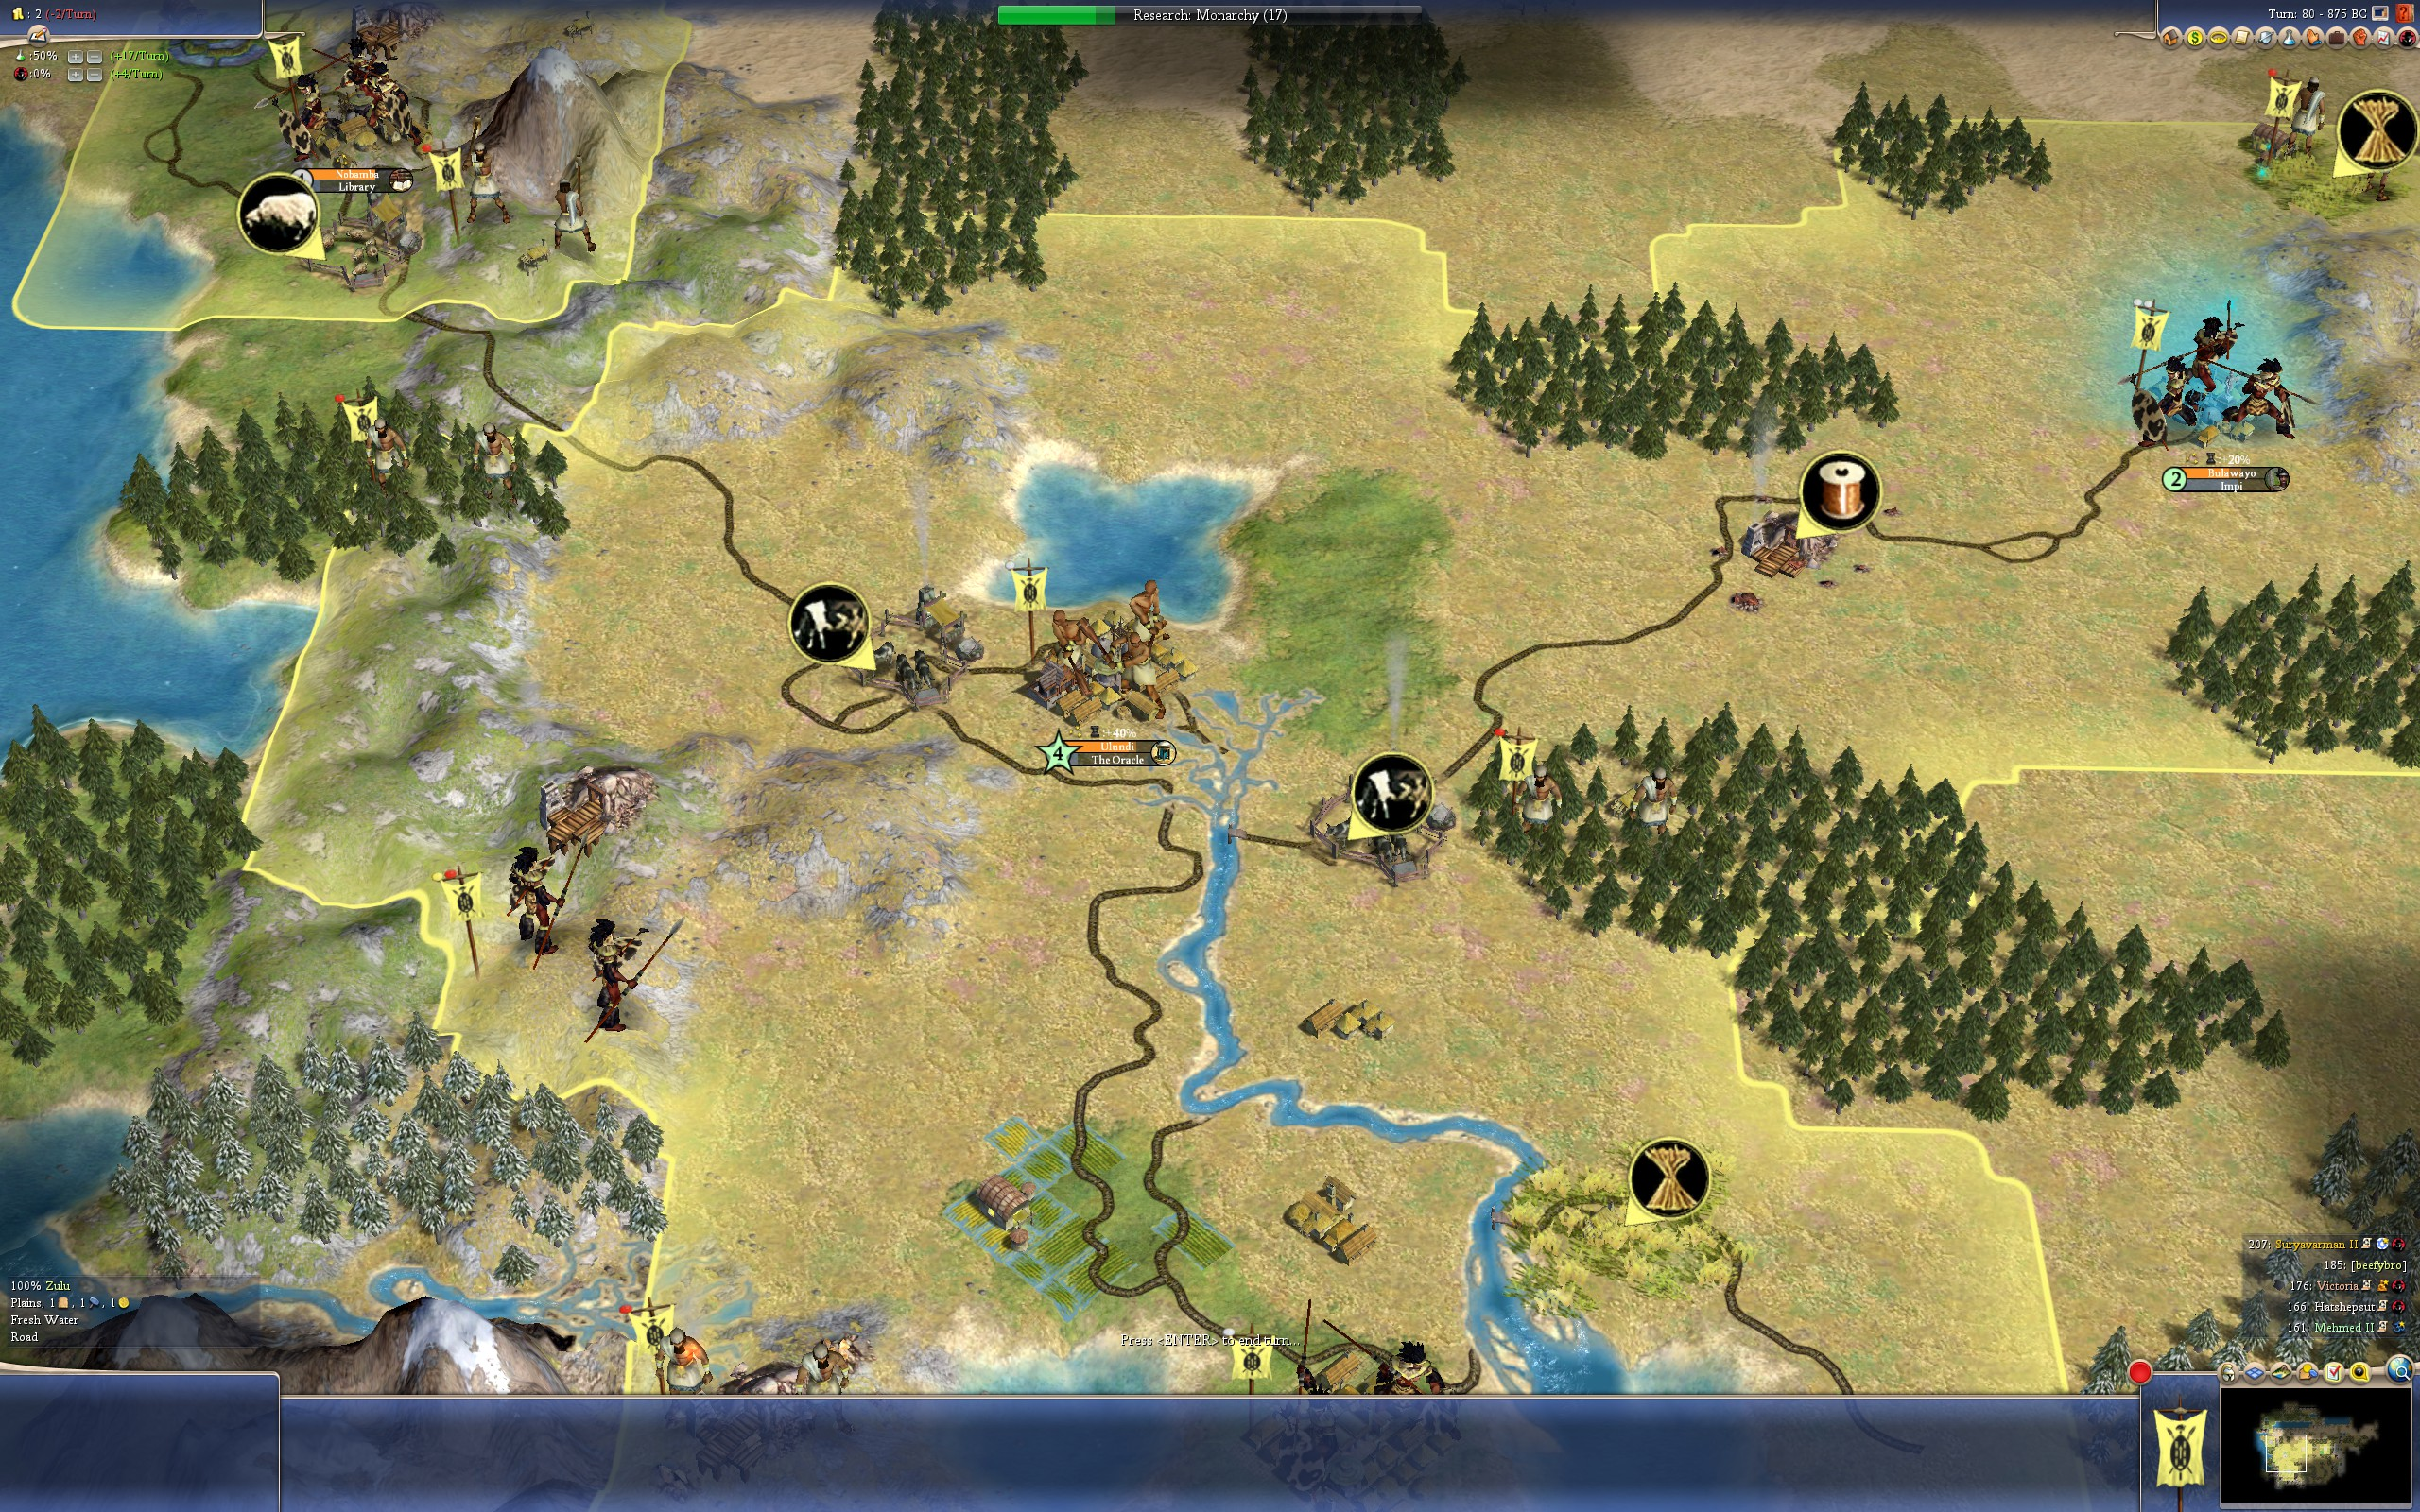
\includegraphics[width=1.0\textwidth]{48}

Despite being very late to Priesthood, the excellent Oracle is still available. My capital is very productive
with the two plains cows and I still have some nearby forests and workers in-place, so I decide to take a
shot at it. An AI builds it shortly after, but at least I get some much-needed gold. The worker to the west
of the cap is outside the BFC but inside my borders. That makes this forest still well-worth chopping.
If you have lots of forests, that's an excellent way to quickly get a wonder (chopping) even if you lack
the bonus resource for that wonder.

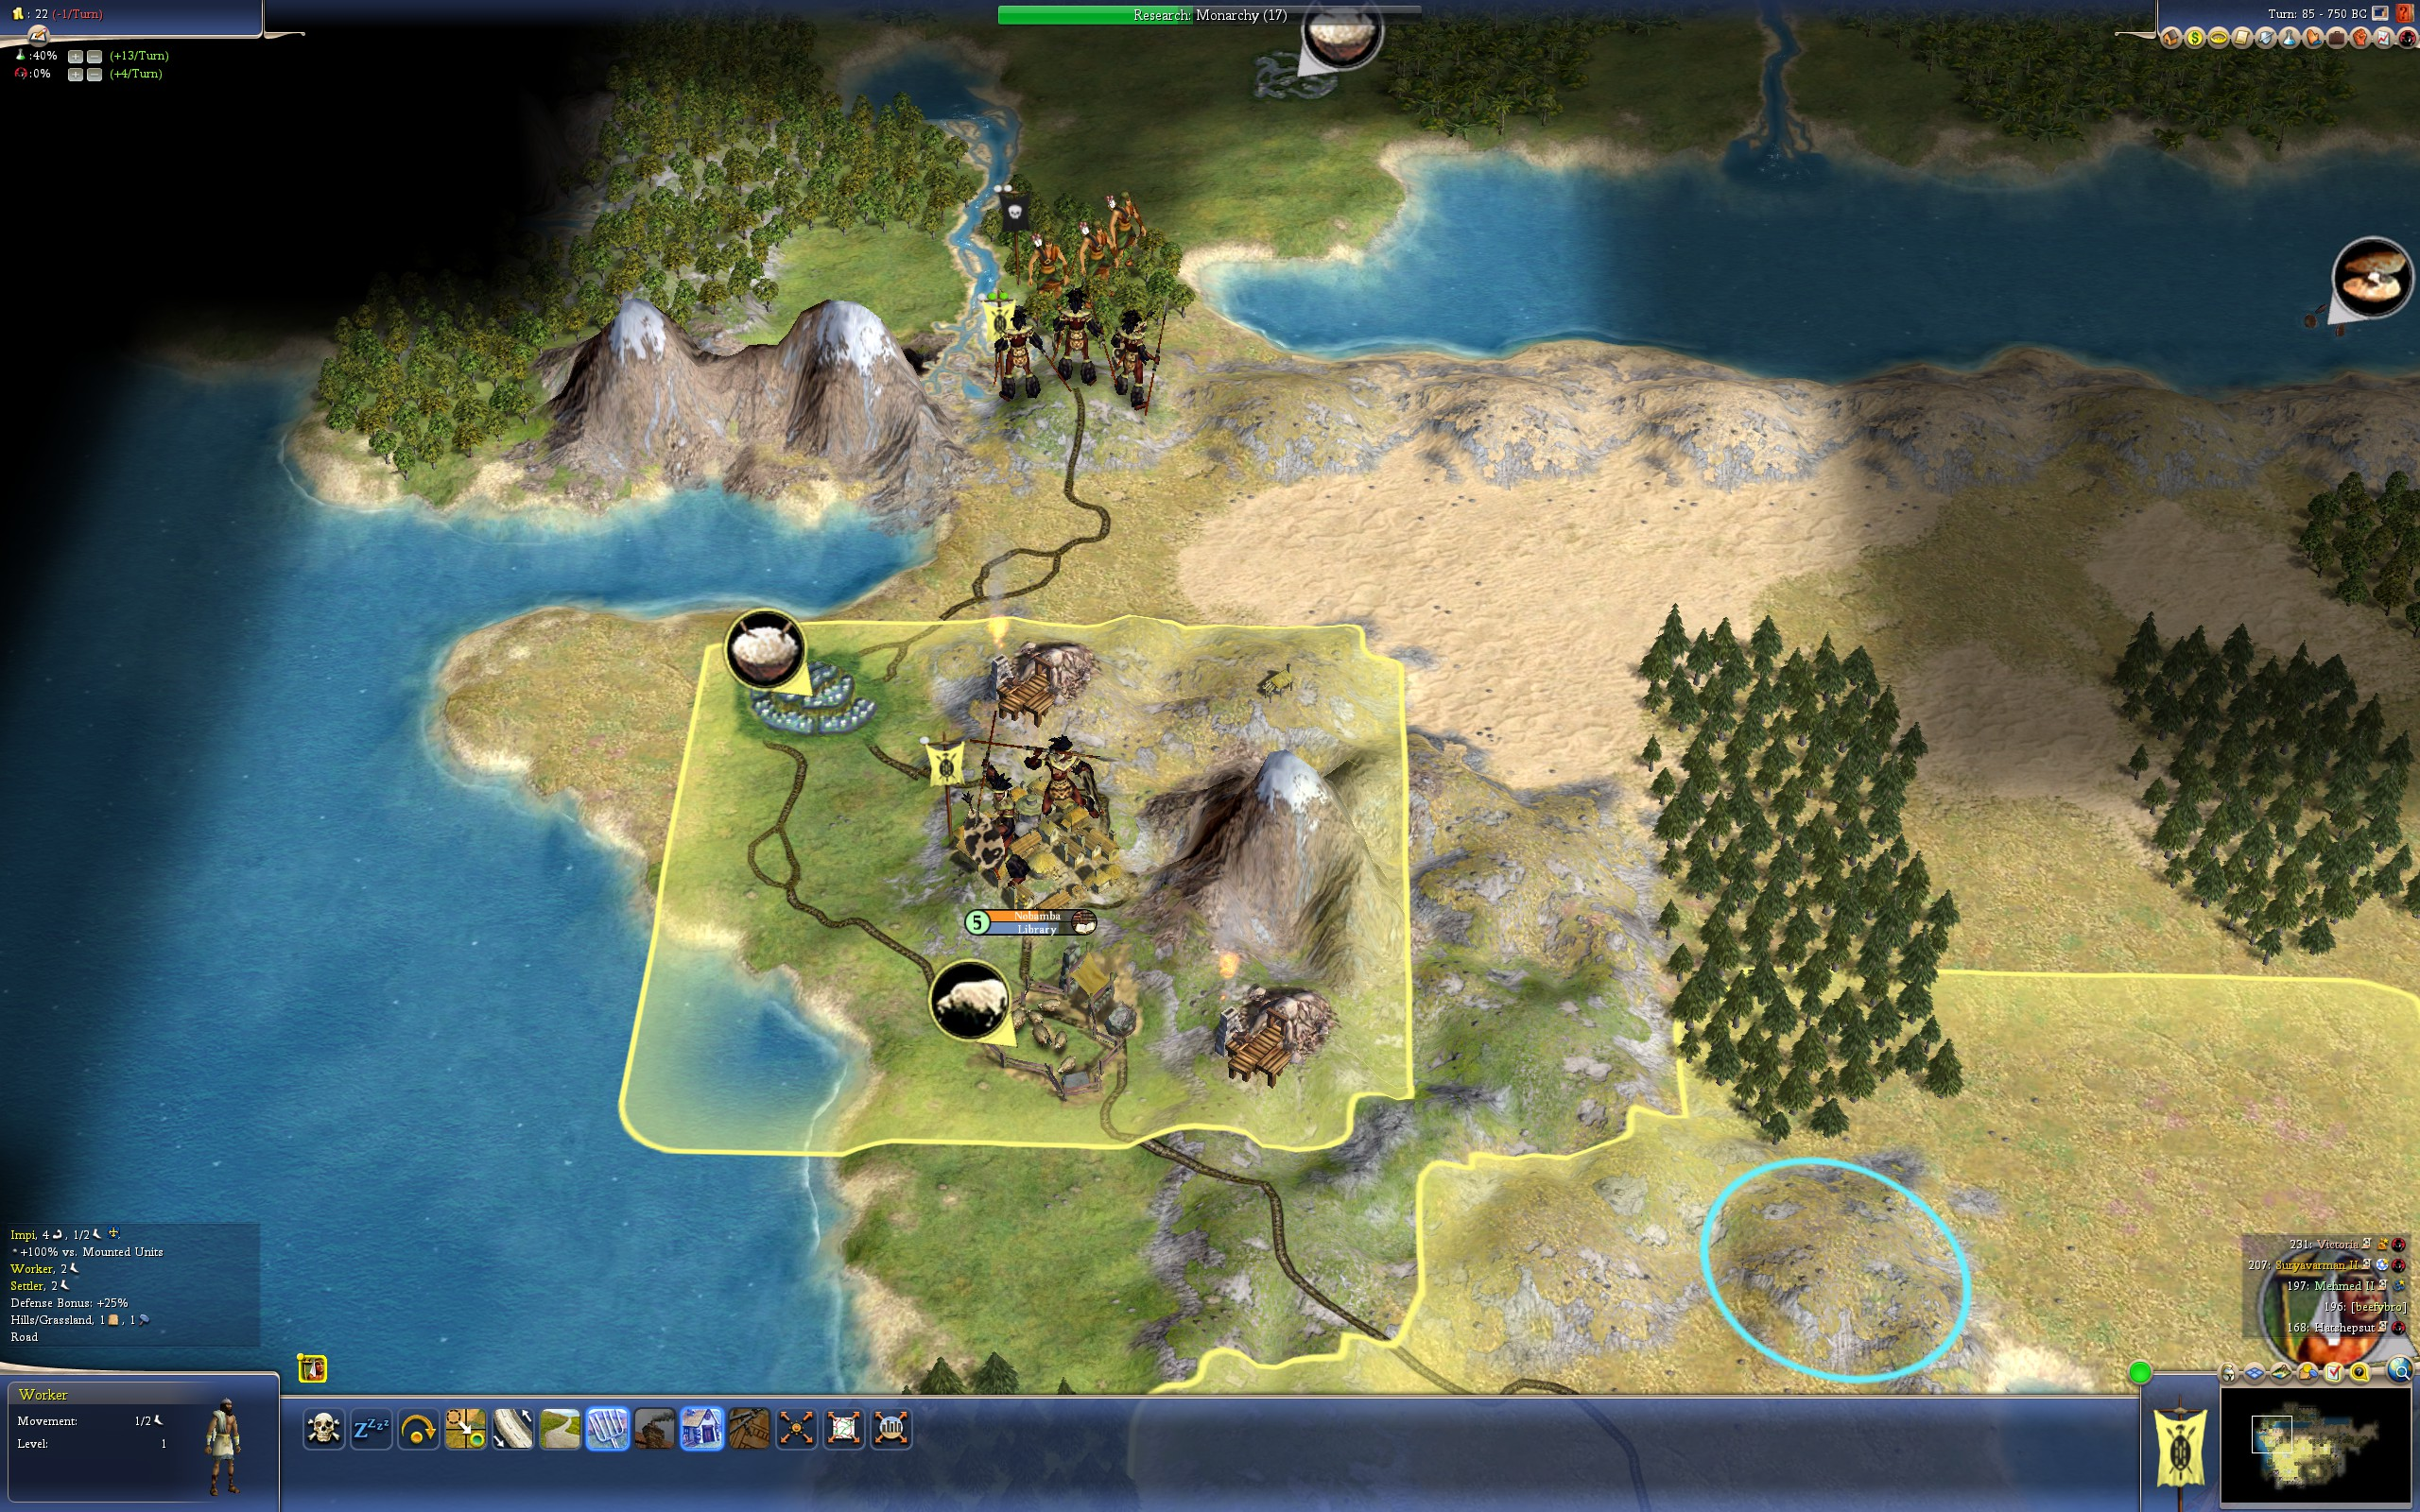
\includegraphics[width=1.0\textwidth]{50}

Here's me trying to grab some of that tasty northern green land. I park my impi on a hill and let the
barbs attack into me for an easy win. Human barbs are not much smarter than animal barbs and are usually
happy to attack into terrible odds.

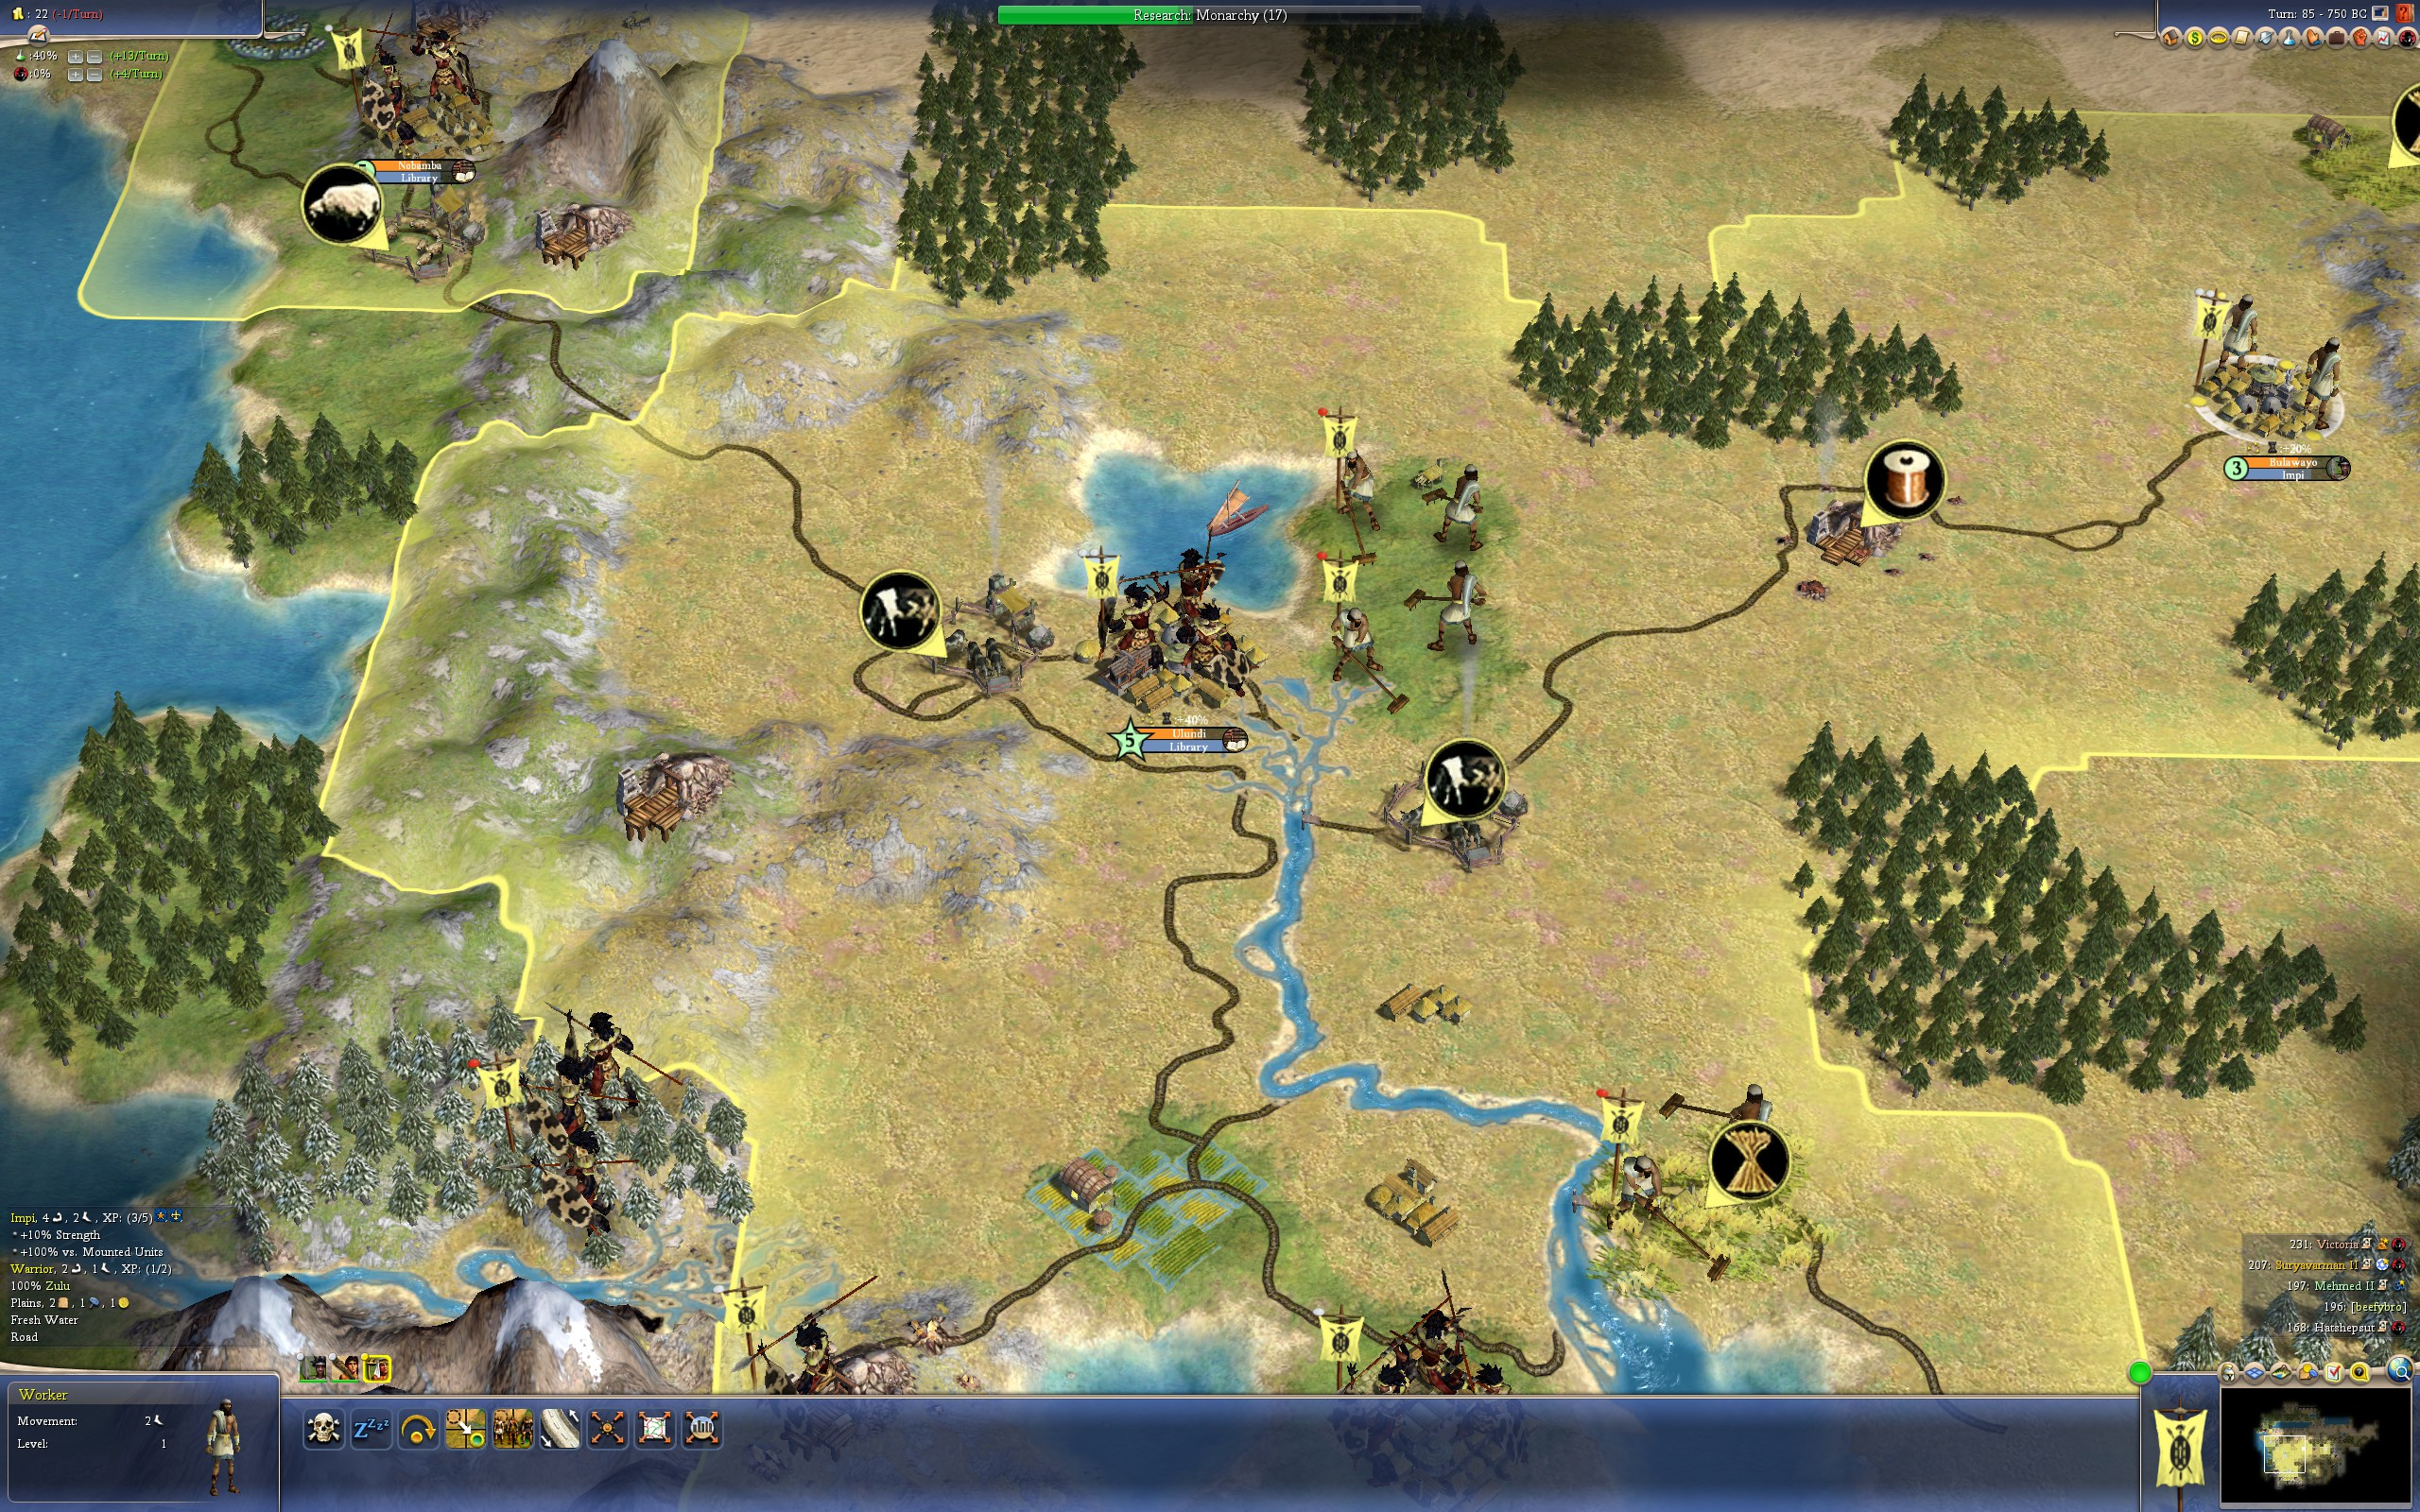
\includegraphics[width=1.0\textwidth]{51}

My capital is ready to grow a bit more but is already having food problems. I have no choice but to farm the
few green tiles I have in order to generate at least a little bit of food surplus.

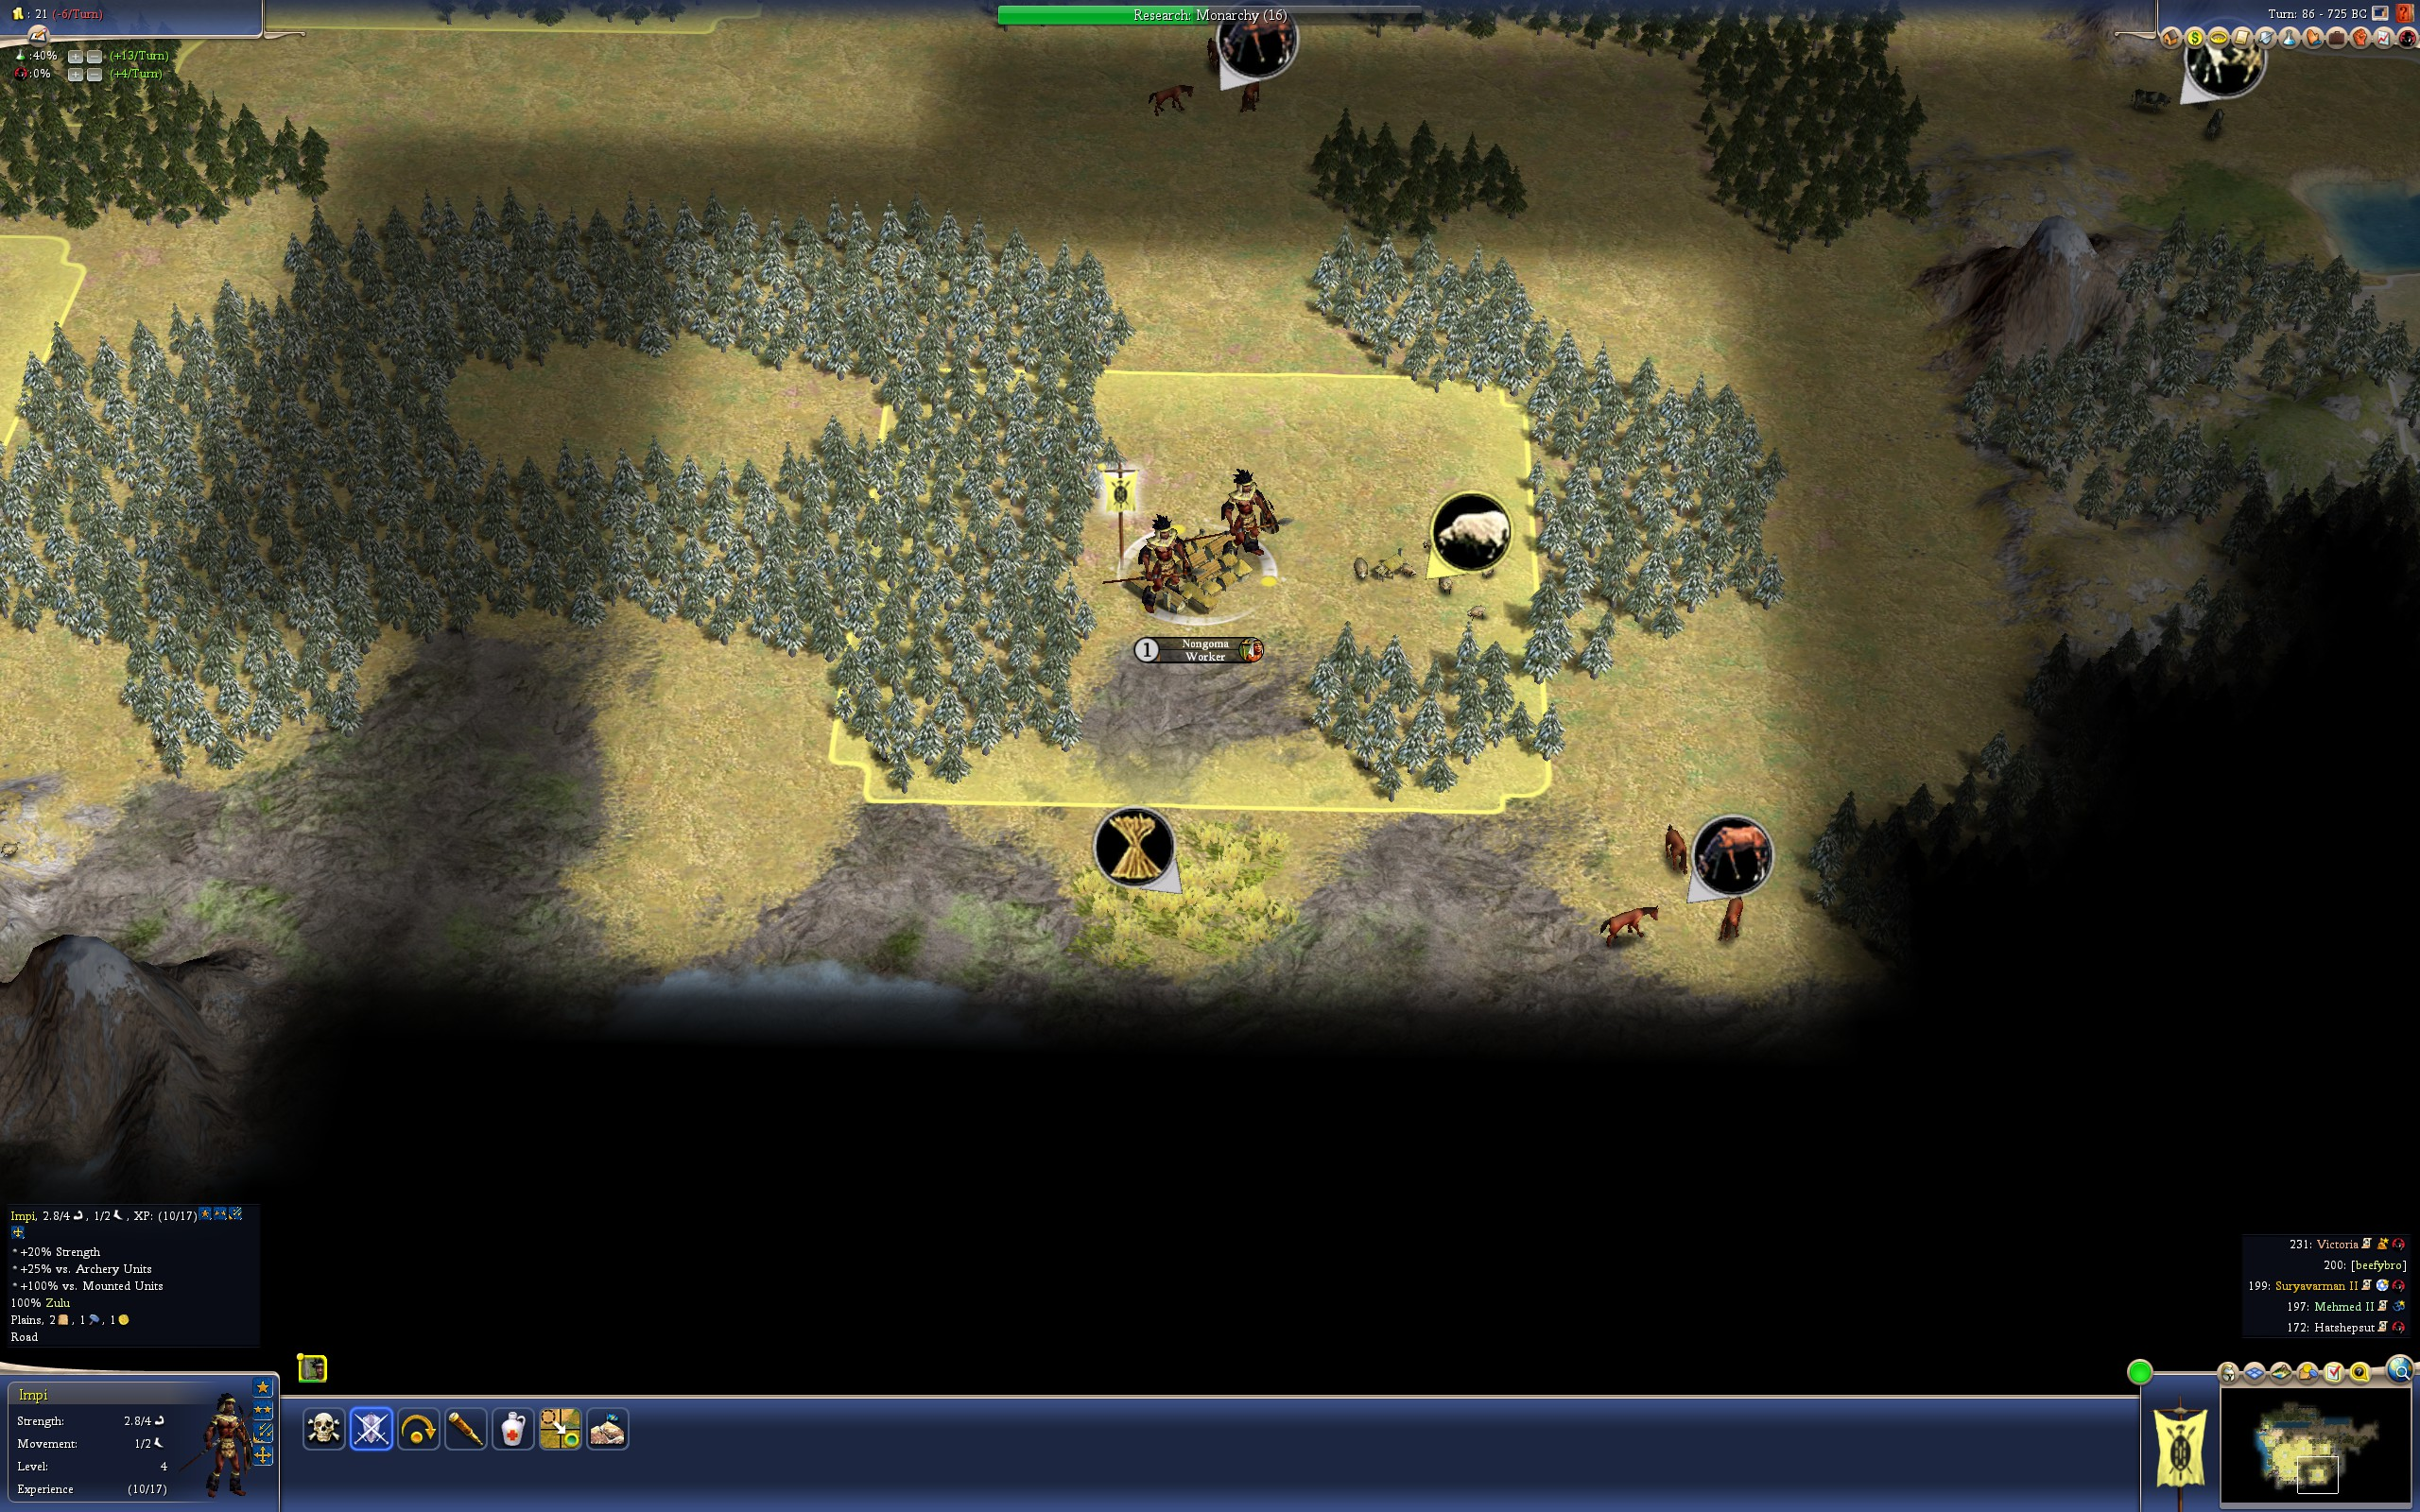
\includegraphics[width=1.0\textwidth]{53}

Another city founded. Looking back on this, I'm not sure why I didn't see 1SE of here. A plains-horse is
a great tile. I think the tundra scared me off, but there's not enough food to work all these plains tiles
anyway.

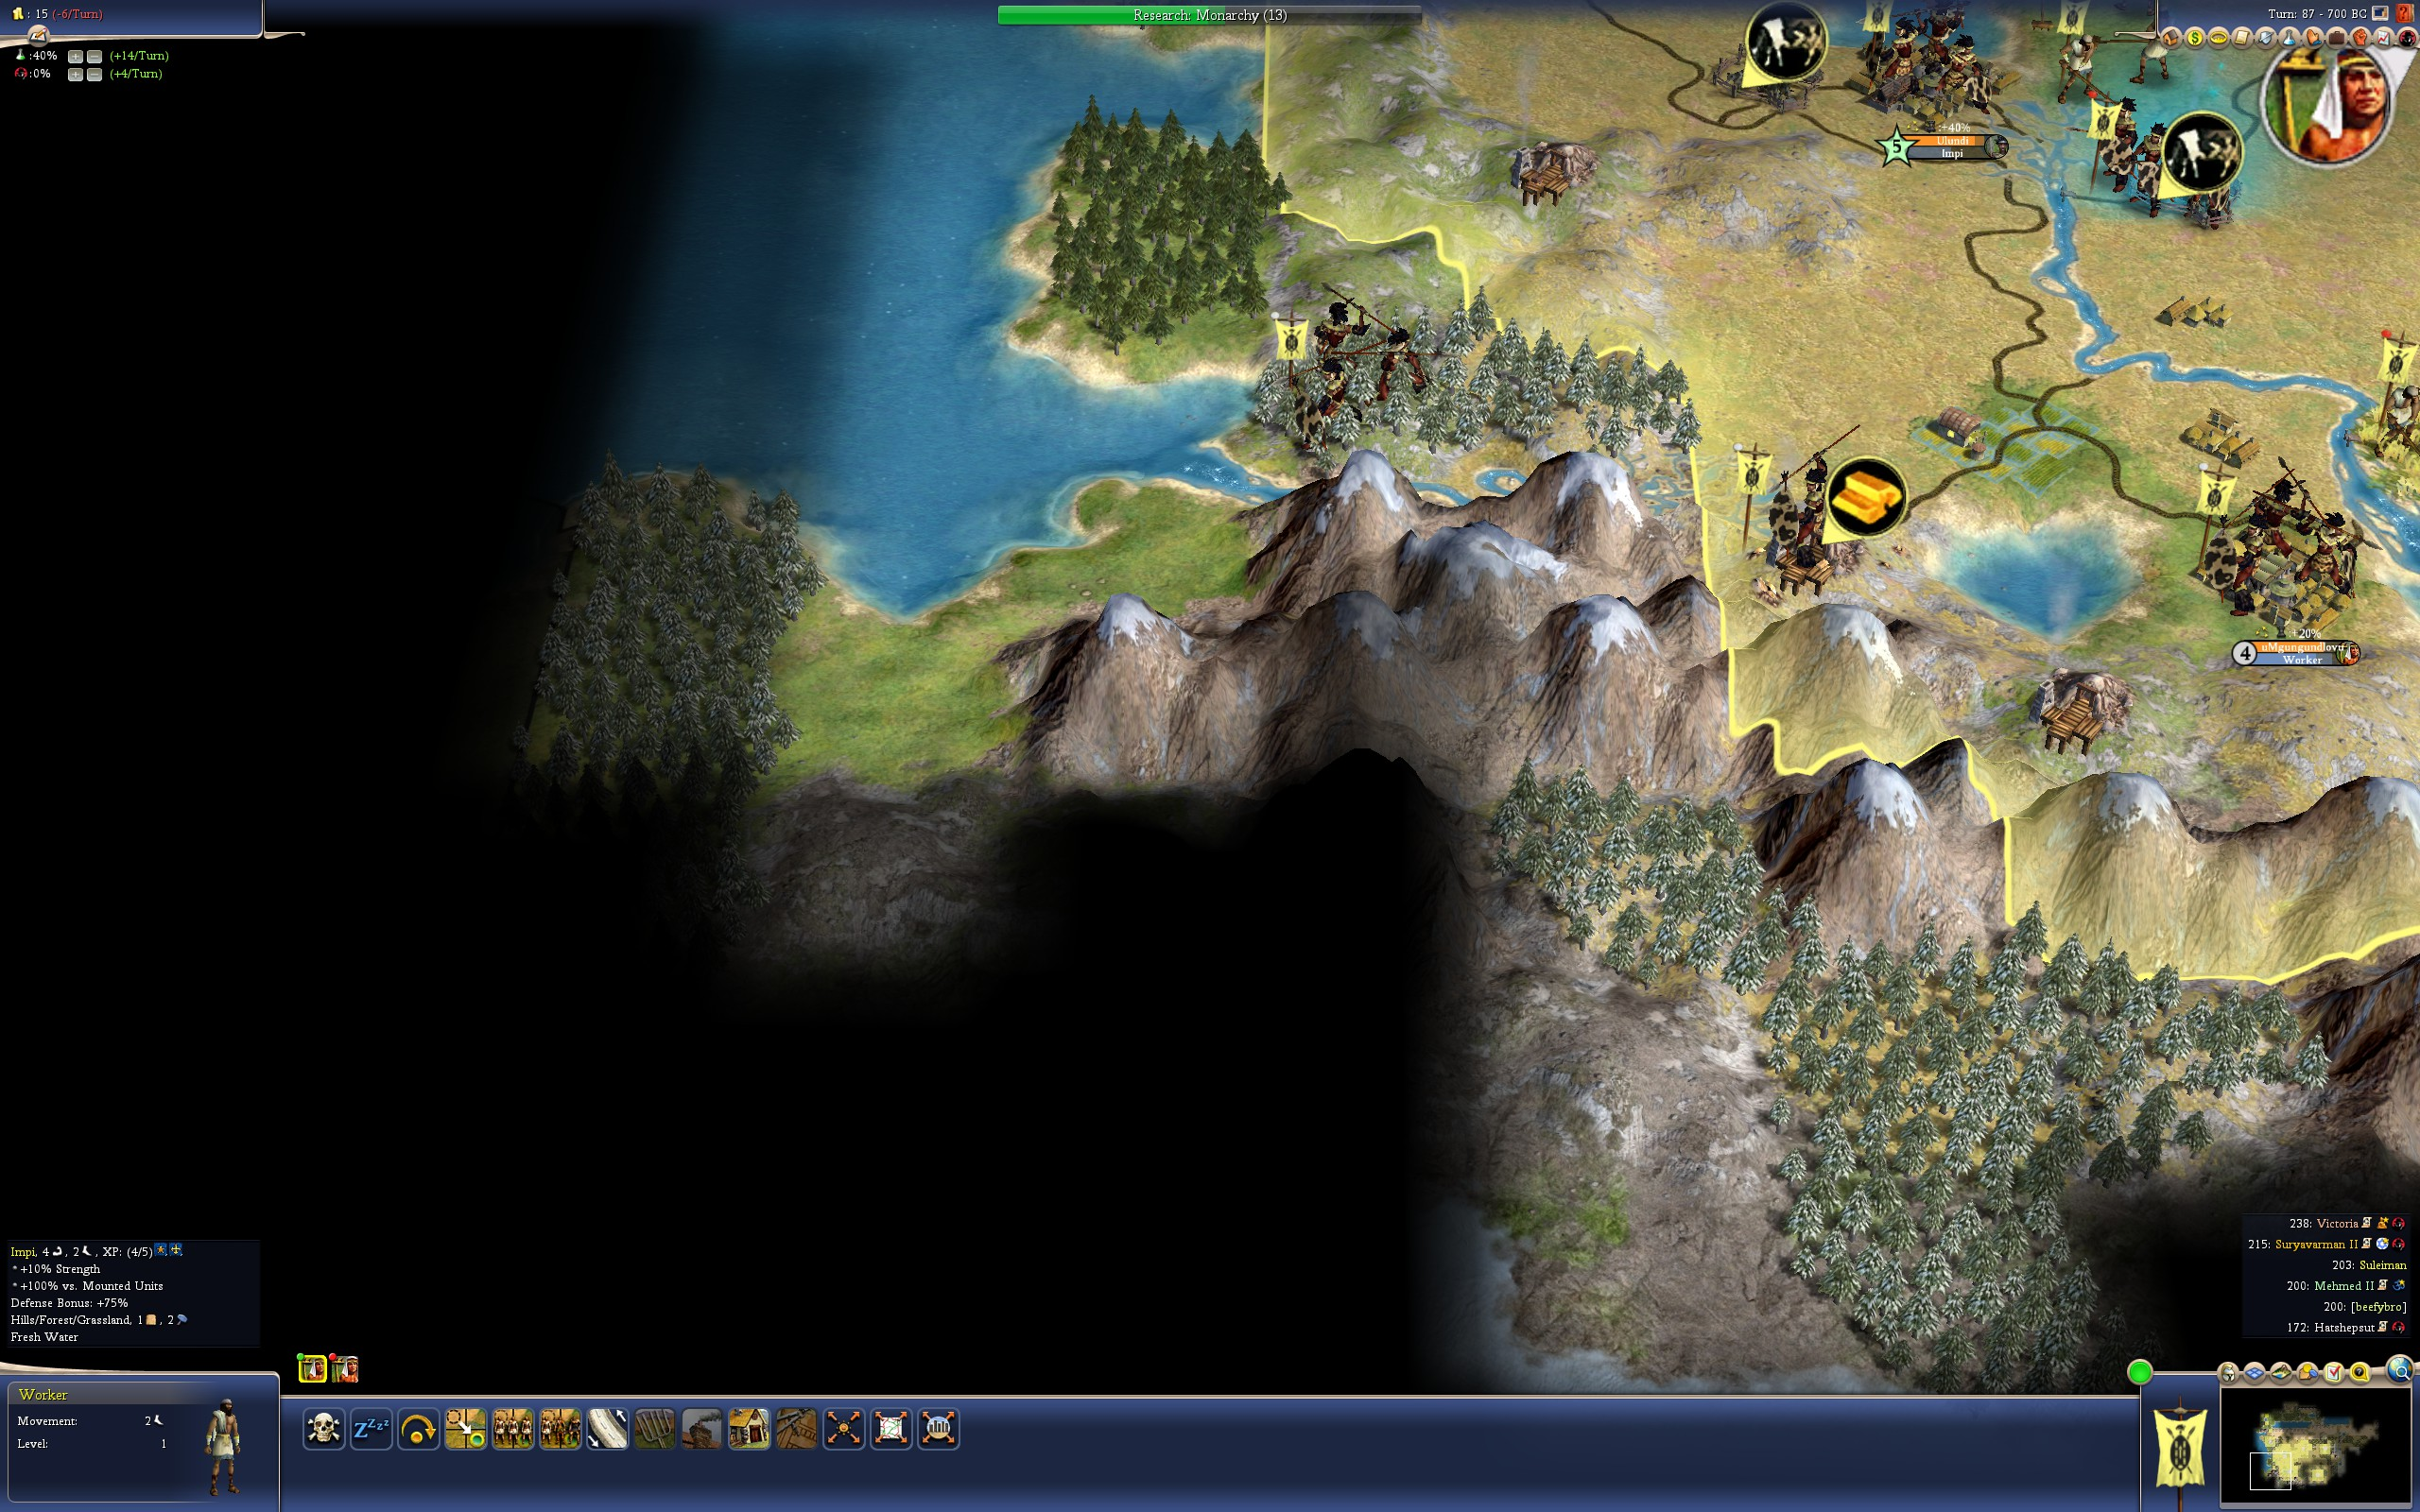
\includegraphics[width=1.0\textwidth]{54}

Here's an impi guarding a choke point to cut off barbs. The cross-river forest guarantees a victory against any
barb that's not an axeman. A lot of barbs have been coming from this direction and this is an efficient way
to cut that off.

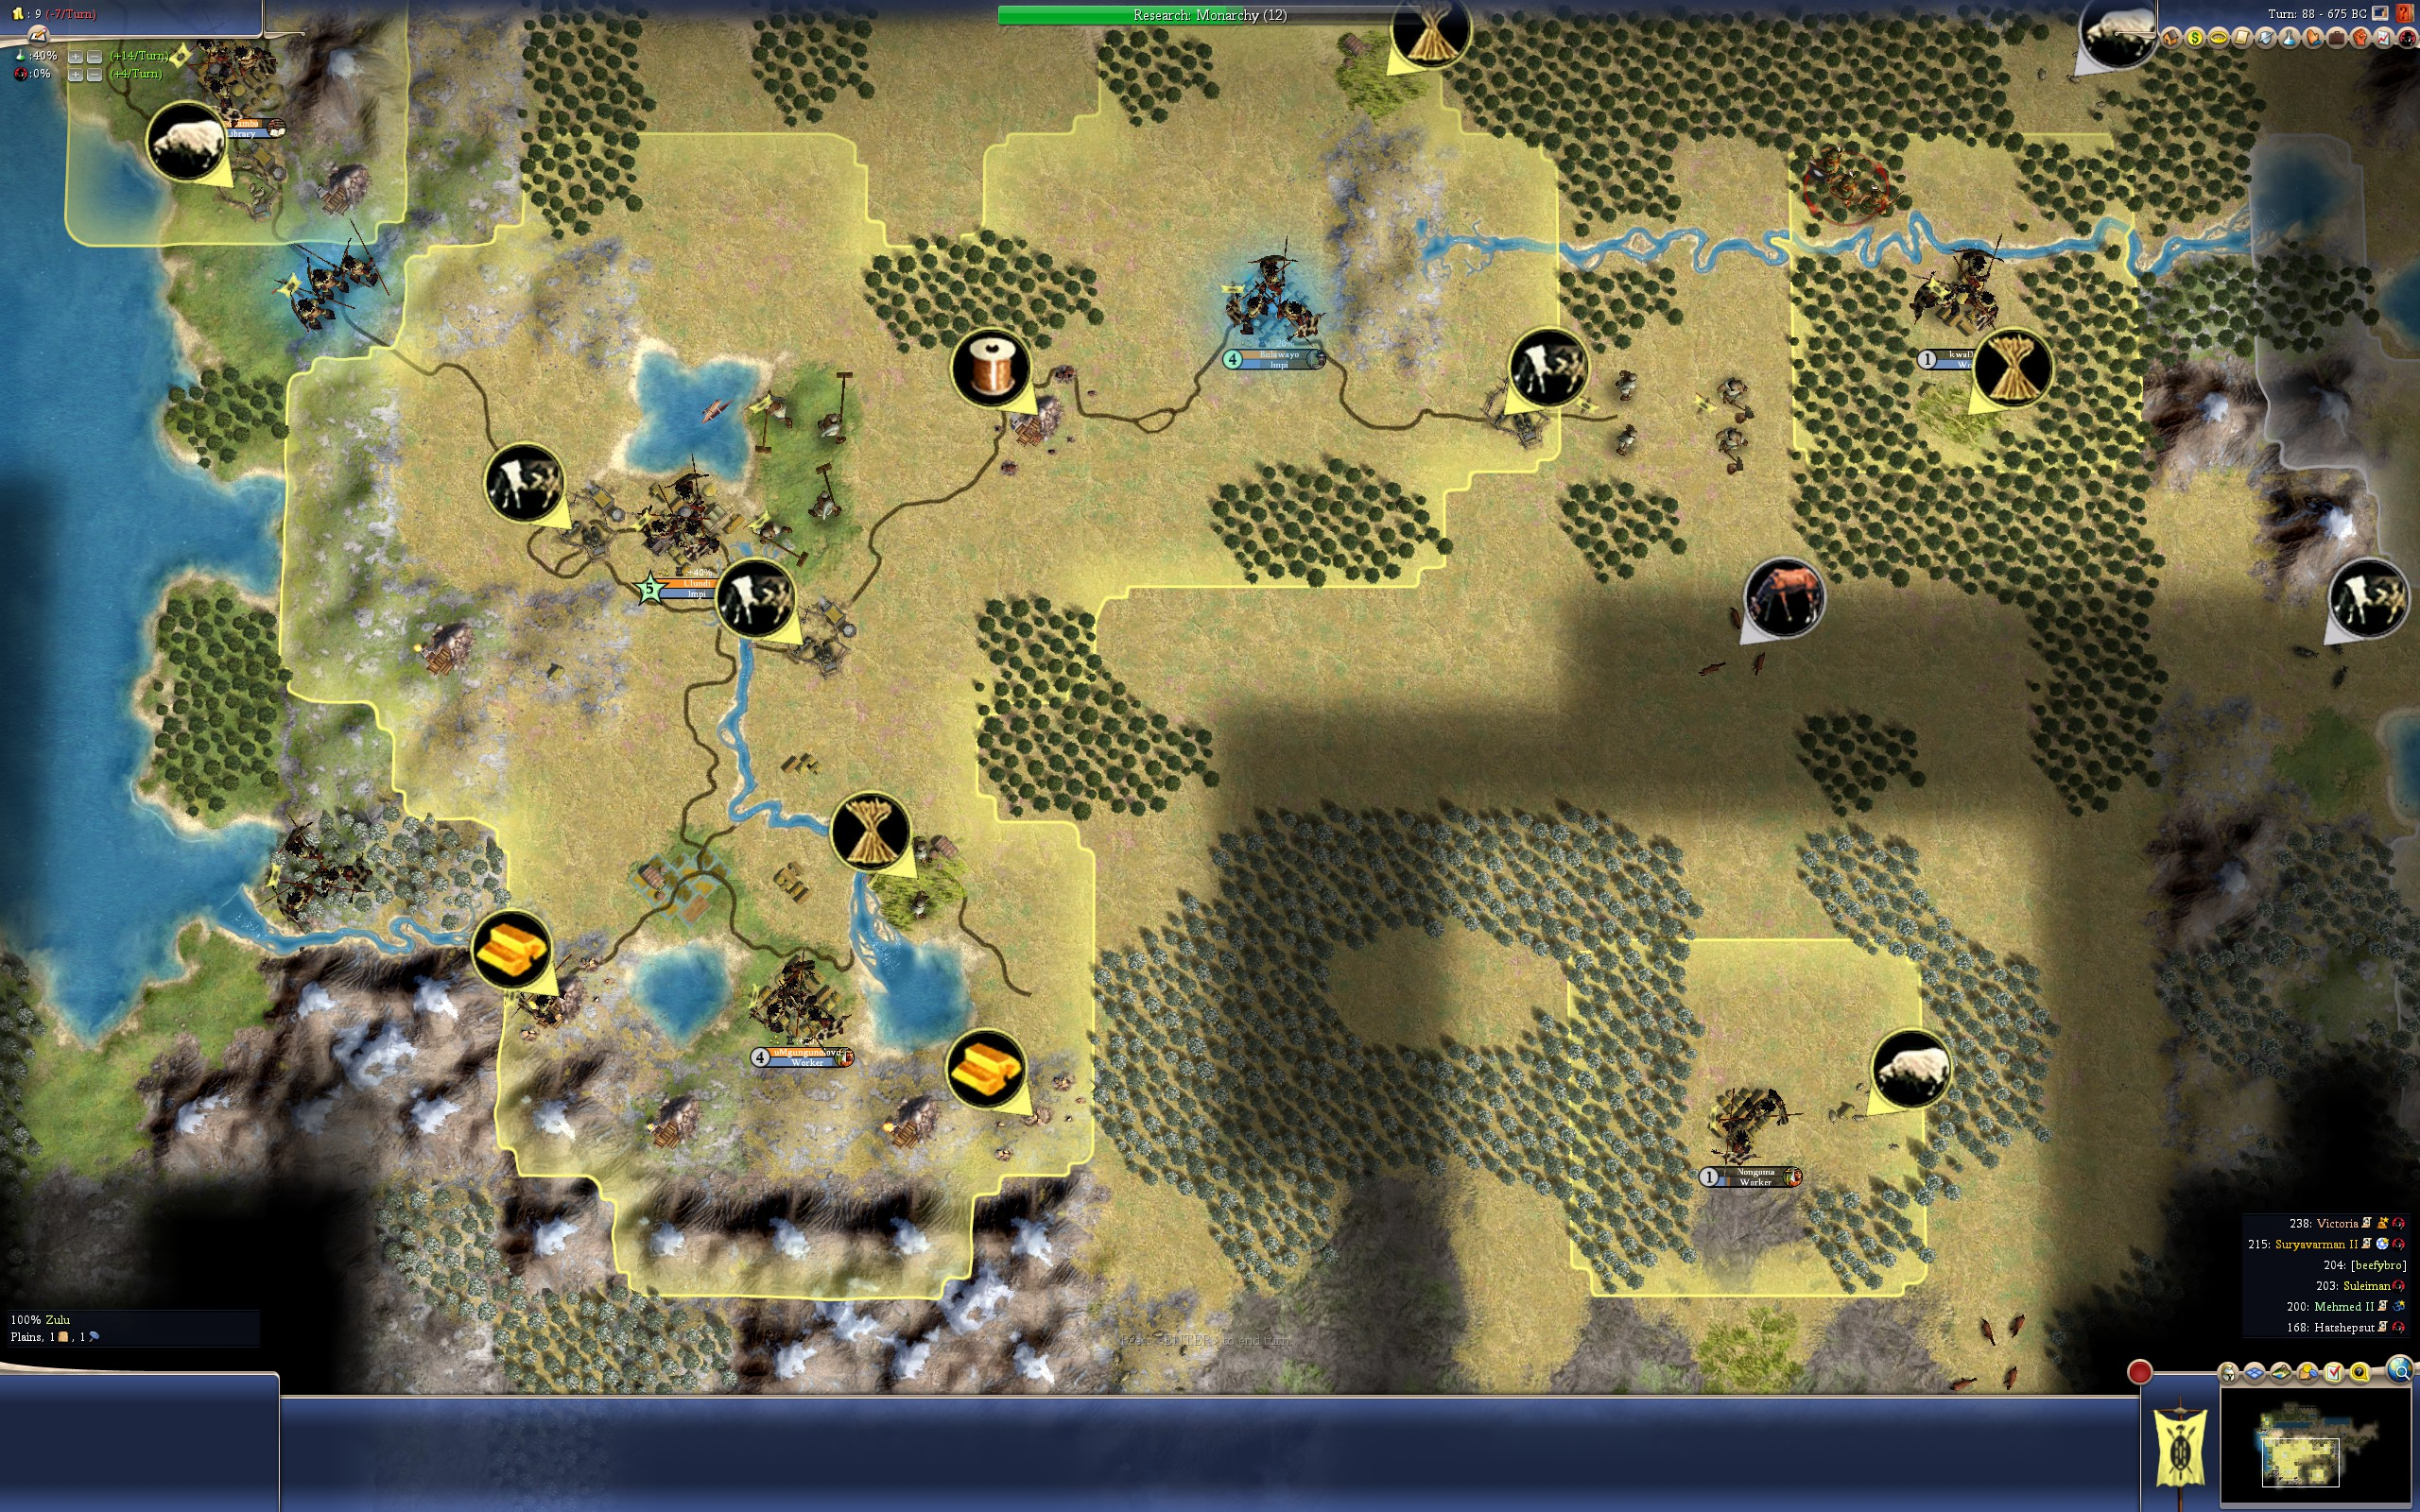
\includegraphics[width=1.0\textwidth]{55}

Overall current lay of the land. My rex is going well thanks to impis.

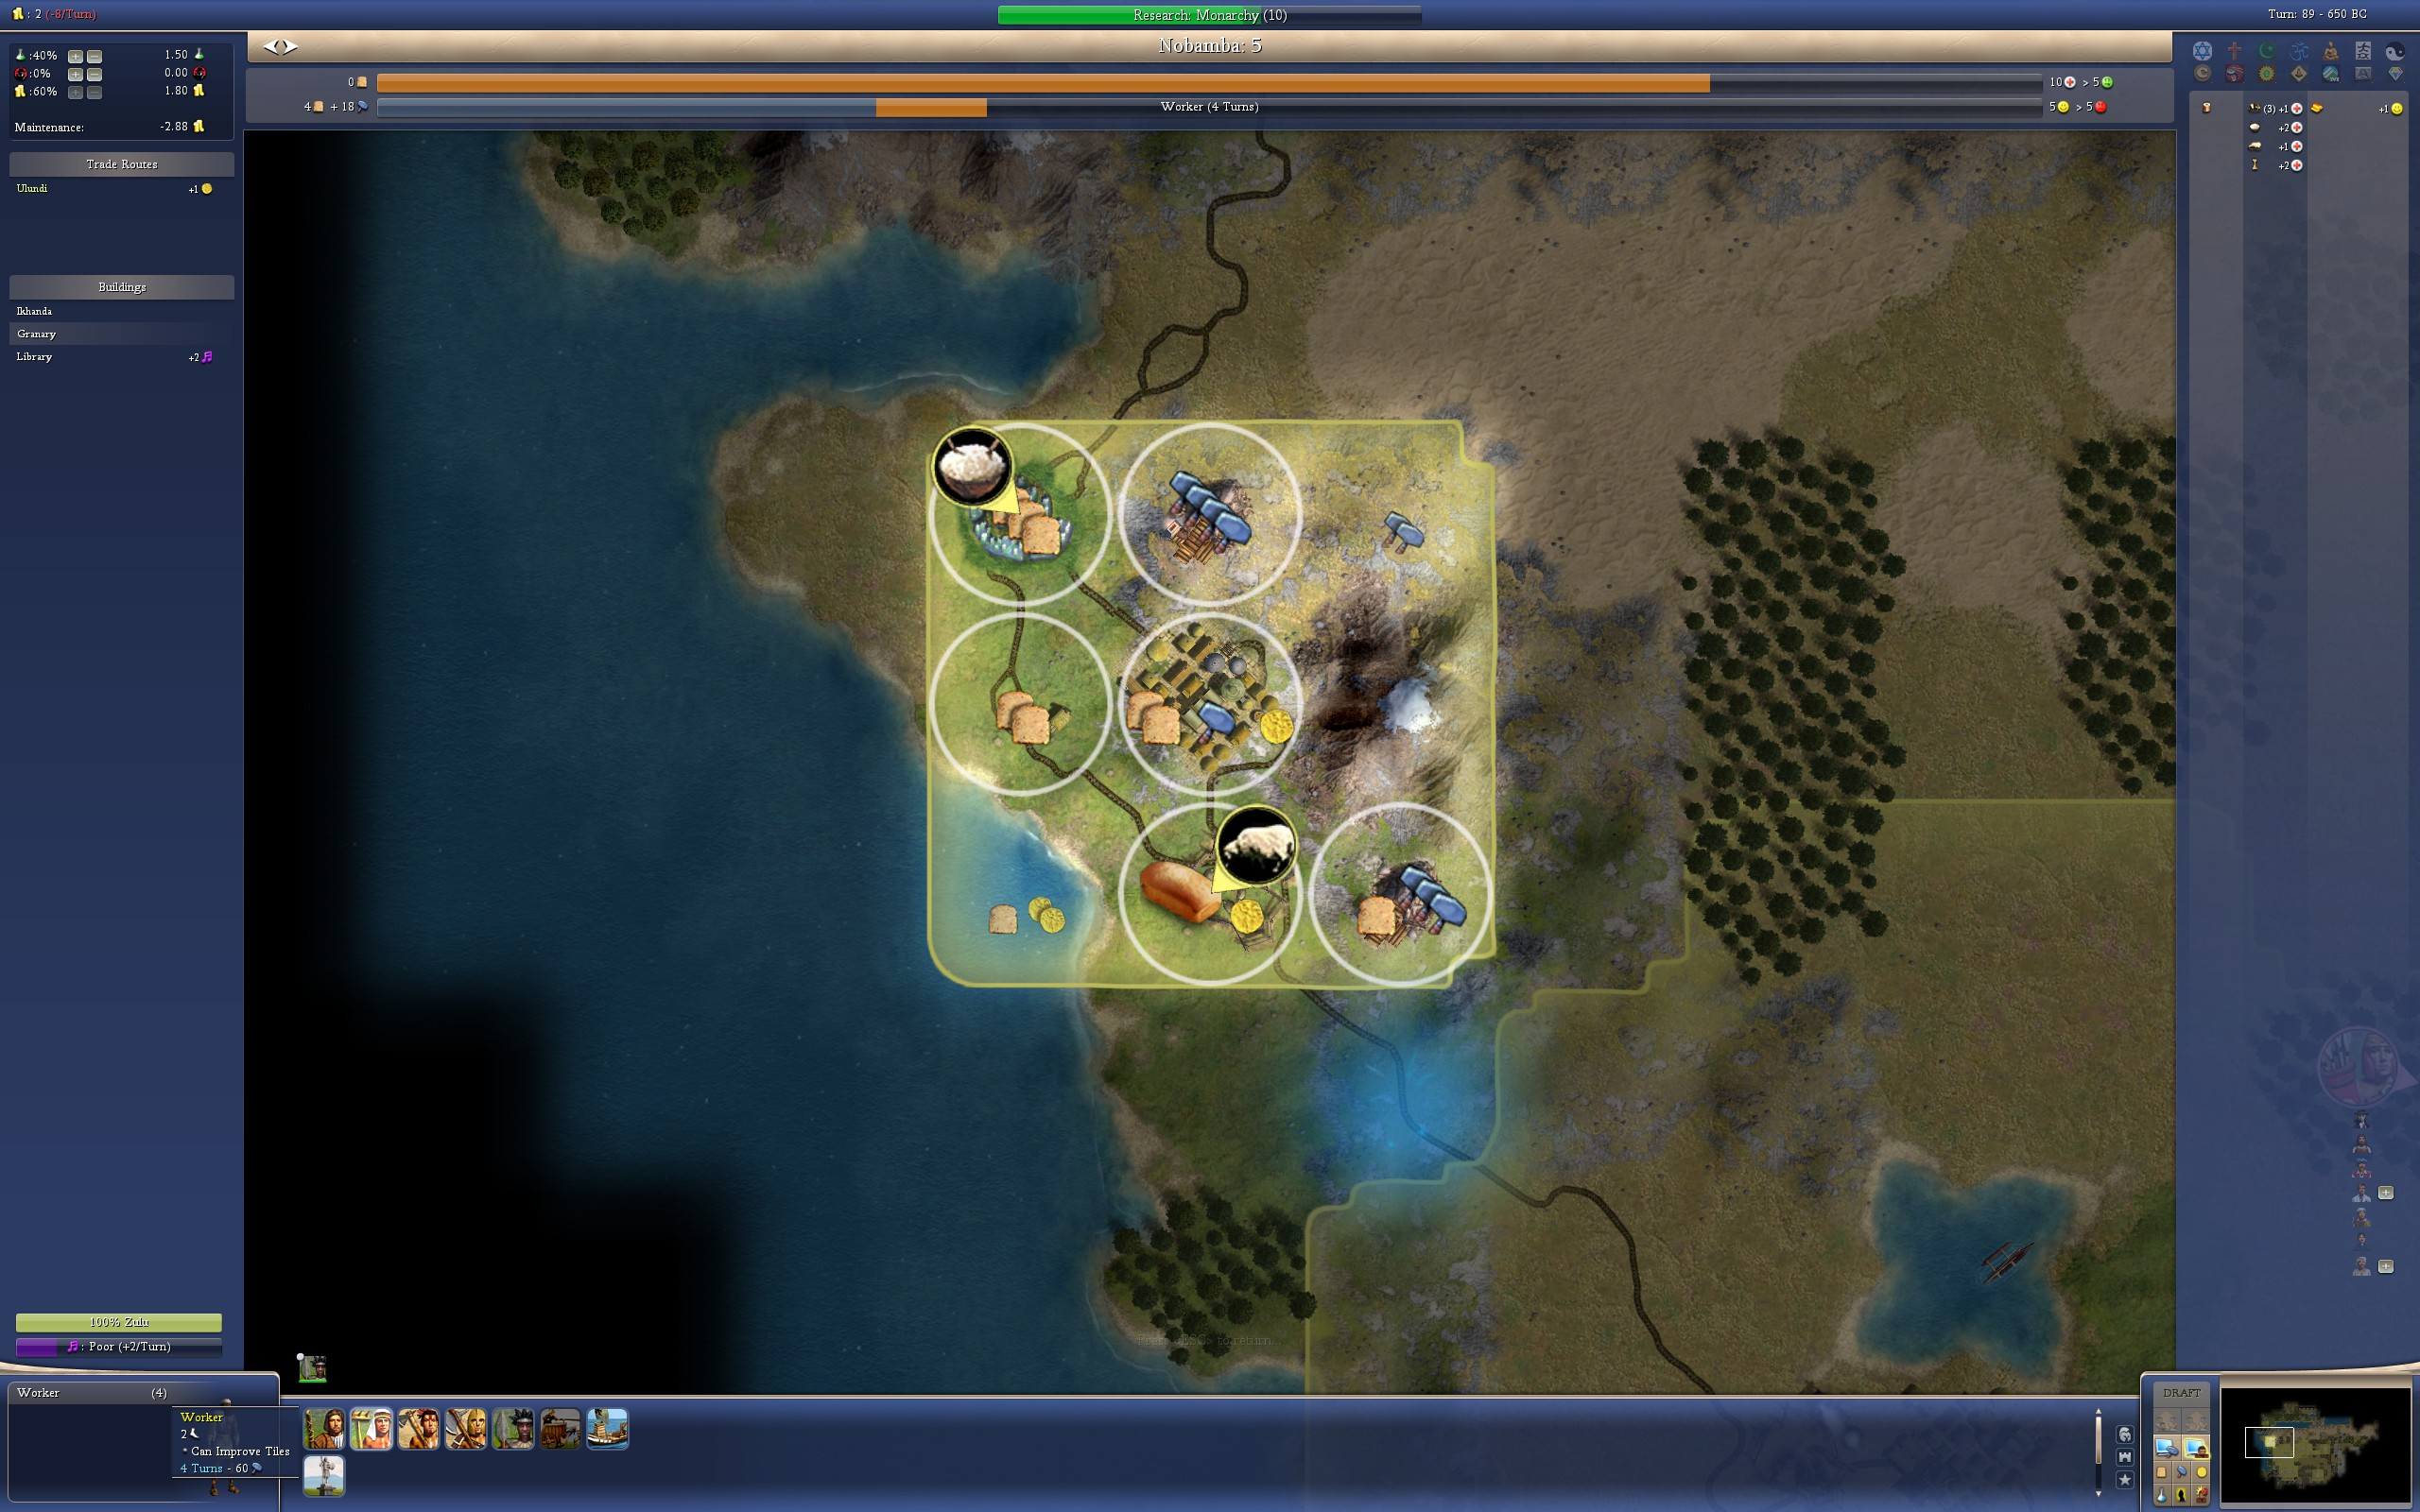
\includegraphics[width=1.0\textwidth]{56}

Just a quick demonstration of a simple technique. If a city is at it's happiness-cap, you may as well build
growth-blocking units because growth won't help you at all. I will need Monarchy before this city can
grow any more. Workers are ALWAYS useful.

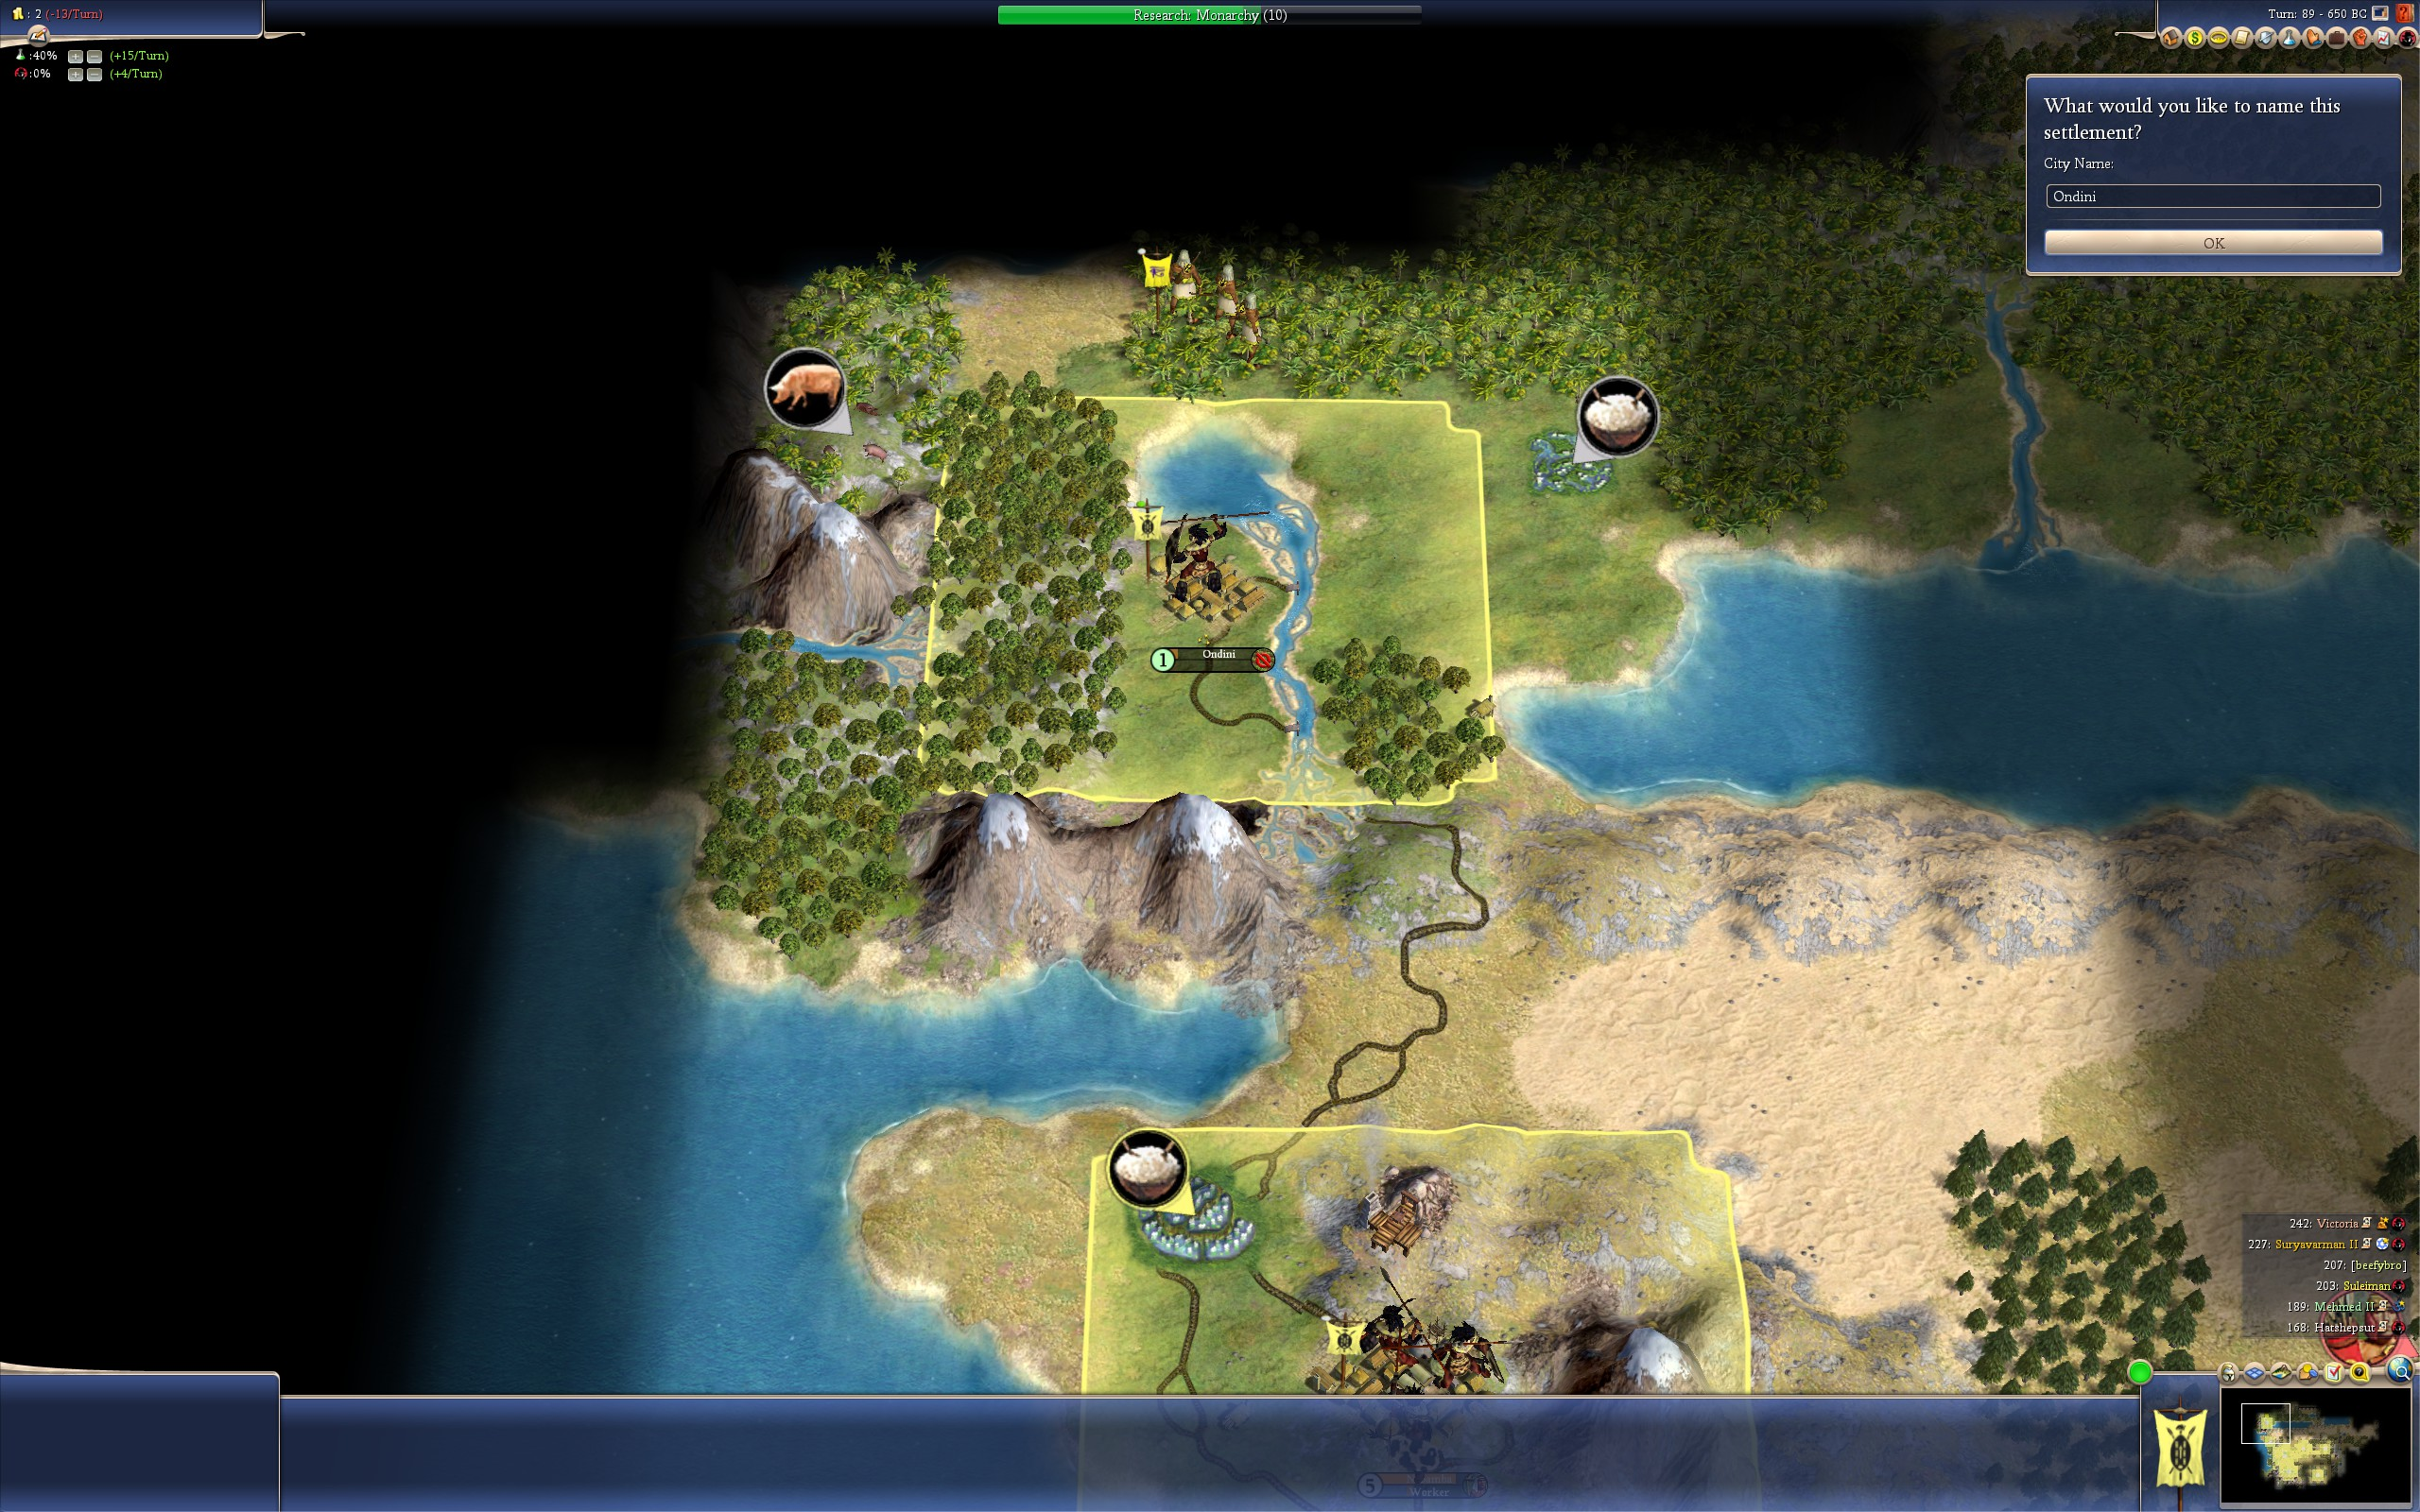
\includegraphics[width=1.0\textwidth]{57}

After fighting off many waves of barbs, an excellent northern city is founded. With two food nodes, several
hills, and lots of green flat tiles that will all be cottaged, this city will be an excellent all-around
commerce city. My best expansion so far.

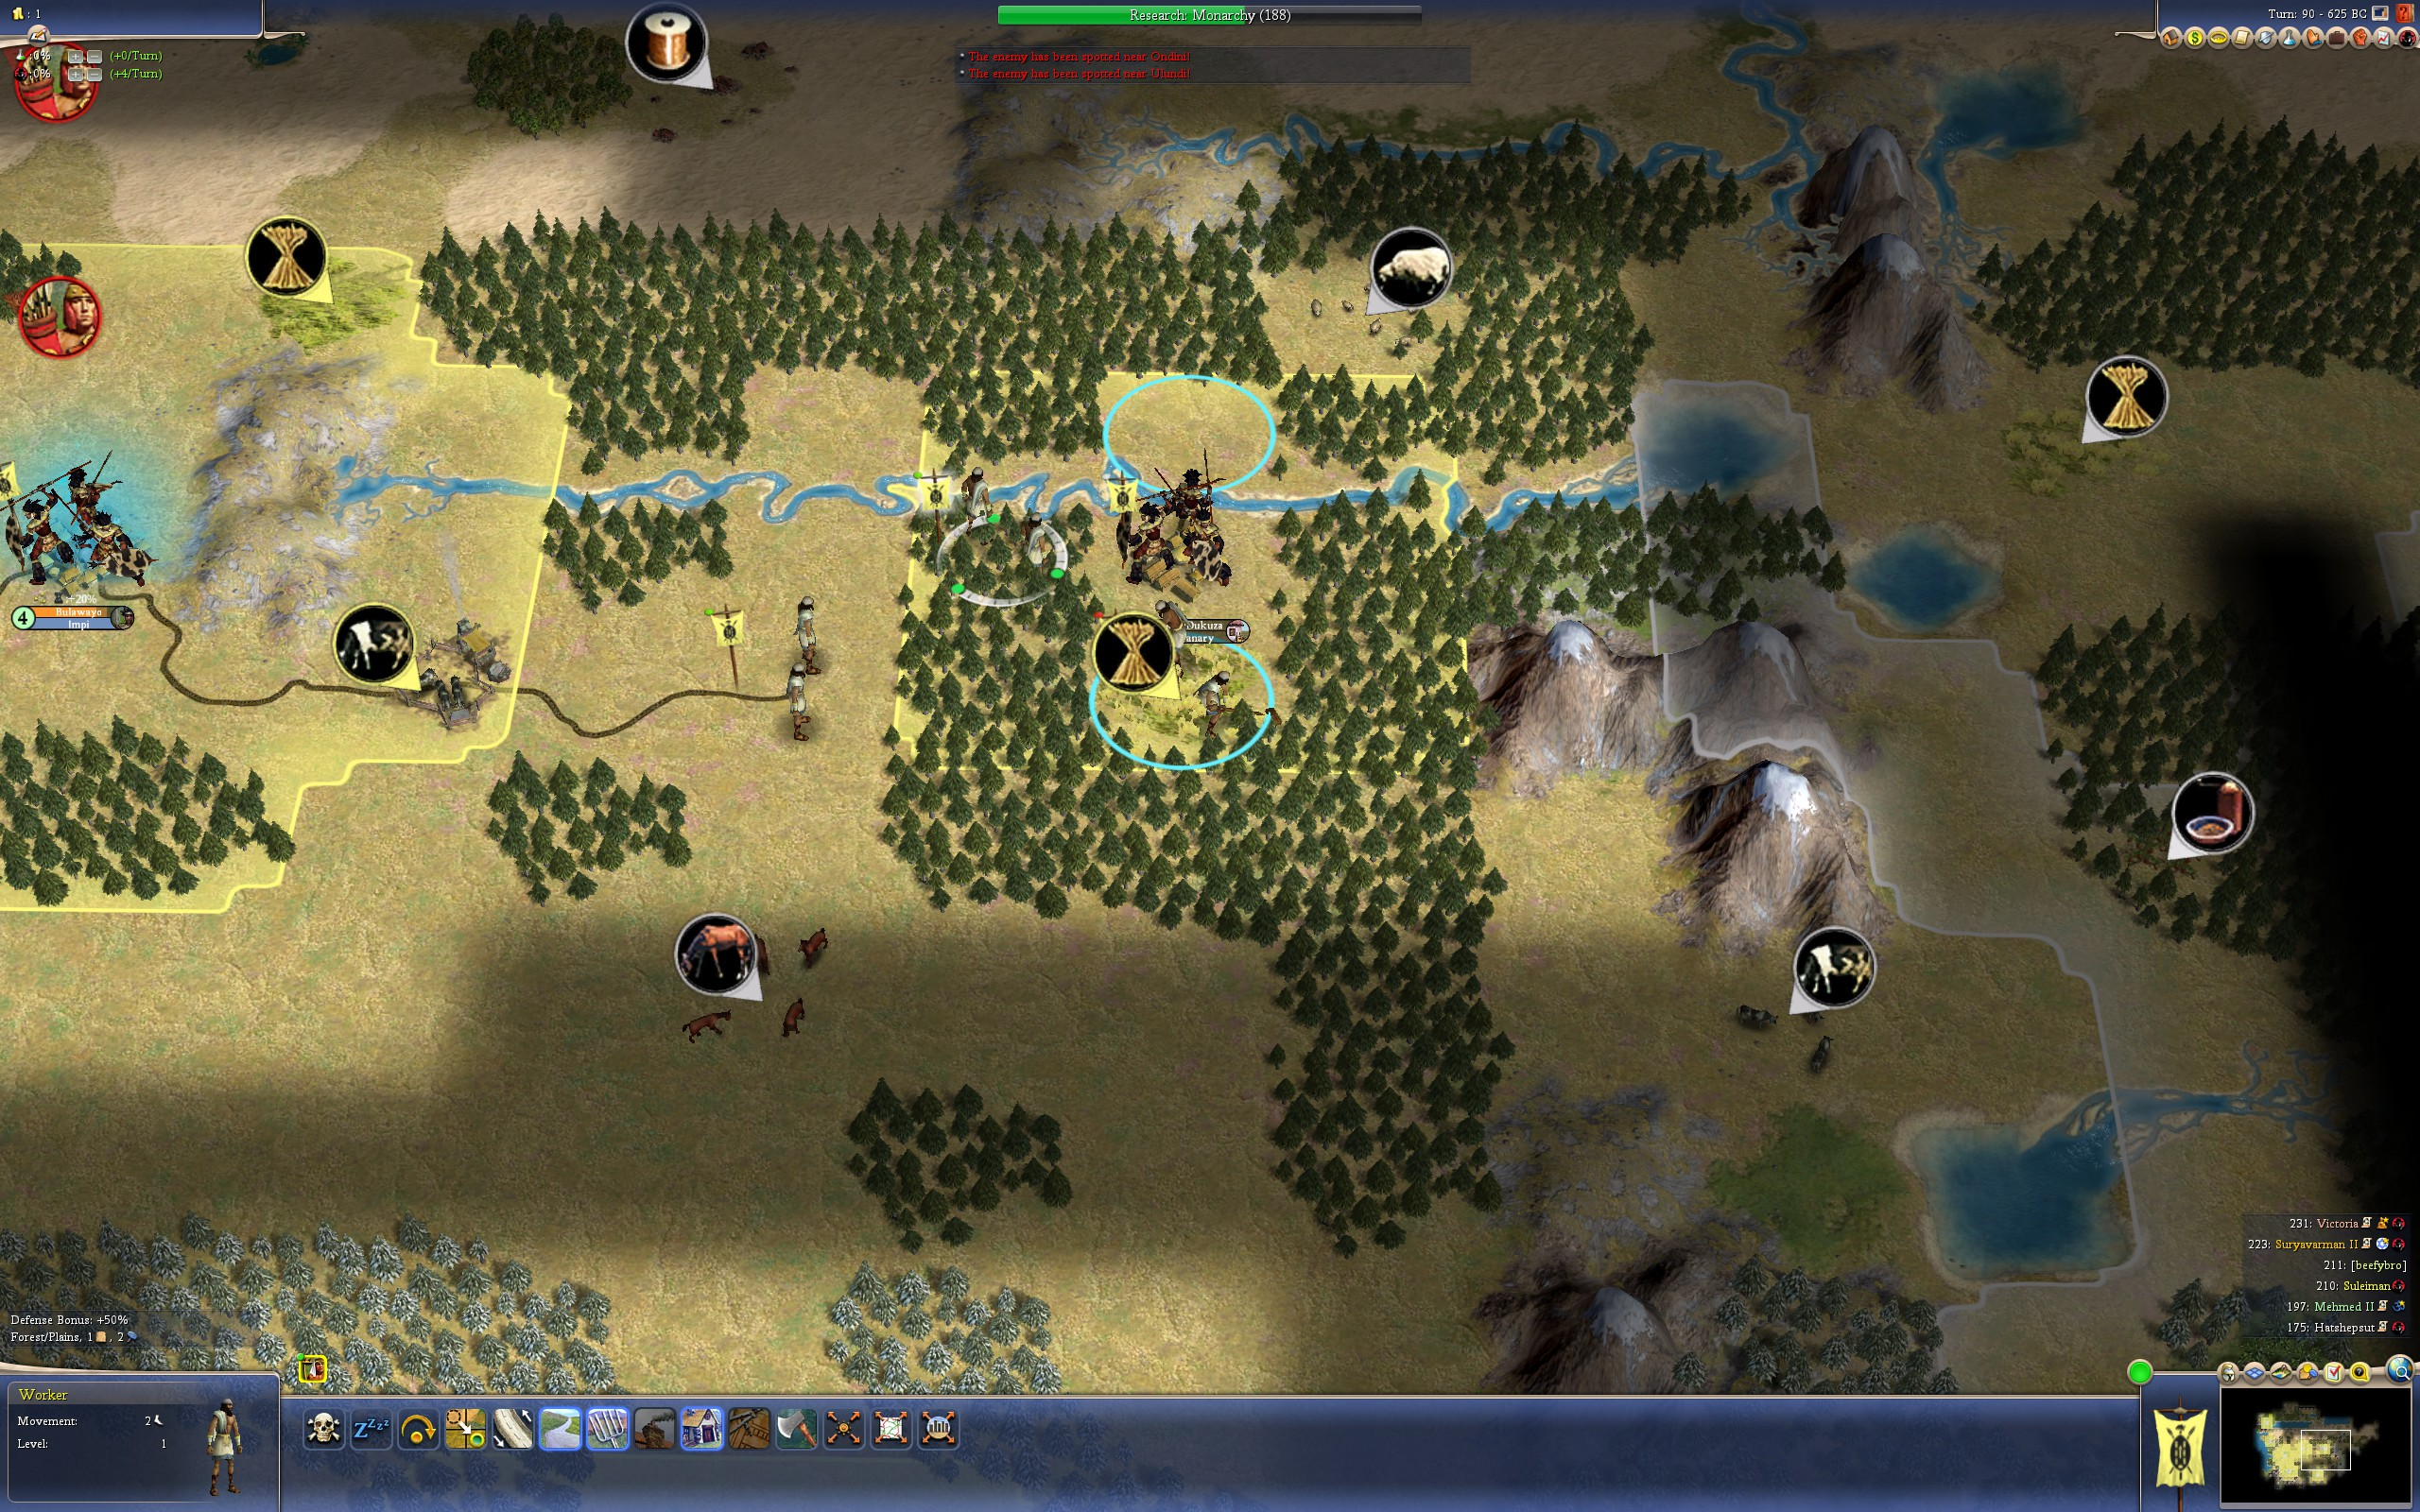
\includegraphics[width=1.0\textwidth]{58}

Due to a fast rex, my economy is offically broken and I'm at 0\% science, not a situation you want to be in
for long! I send a surge of workers east in order to establish a trade connection with Hatty. Foreign routes
give about 2x the commerce of a local route and I desperately need commerce at this point to ressurect my
economy, so this is a top priority.

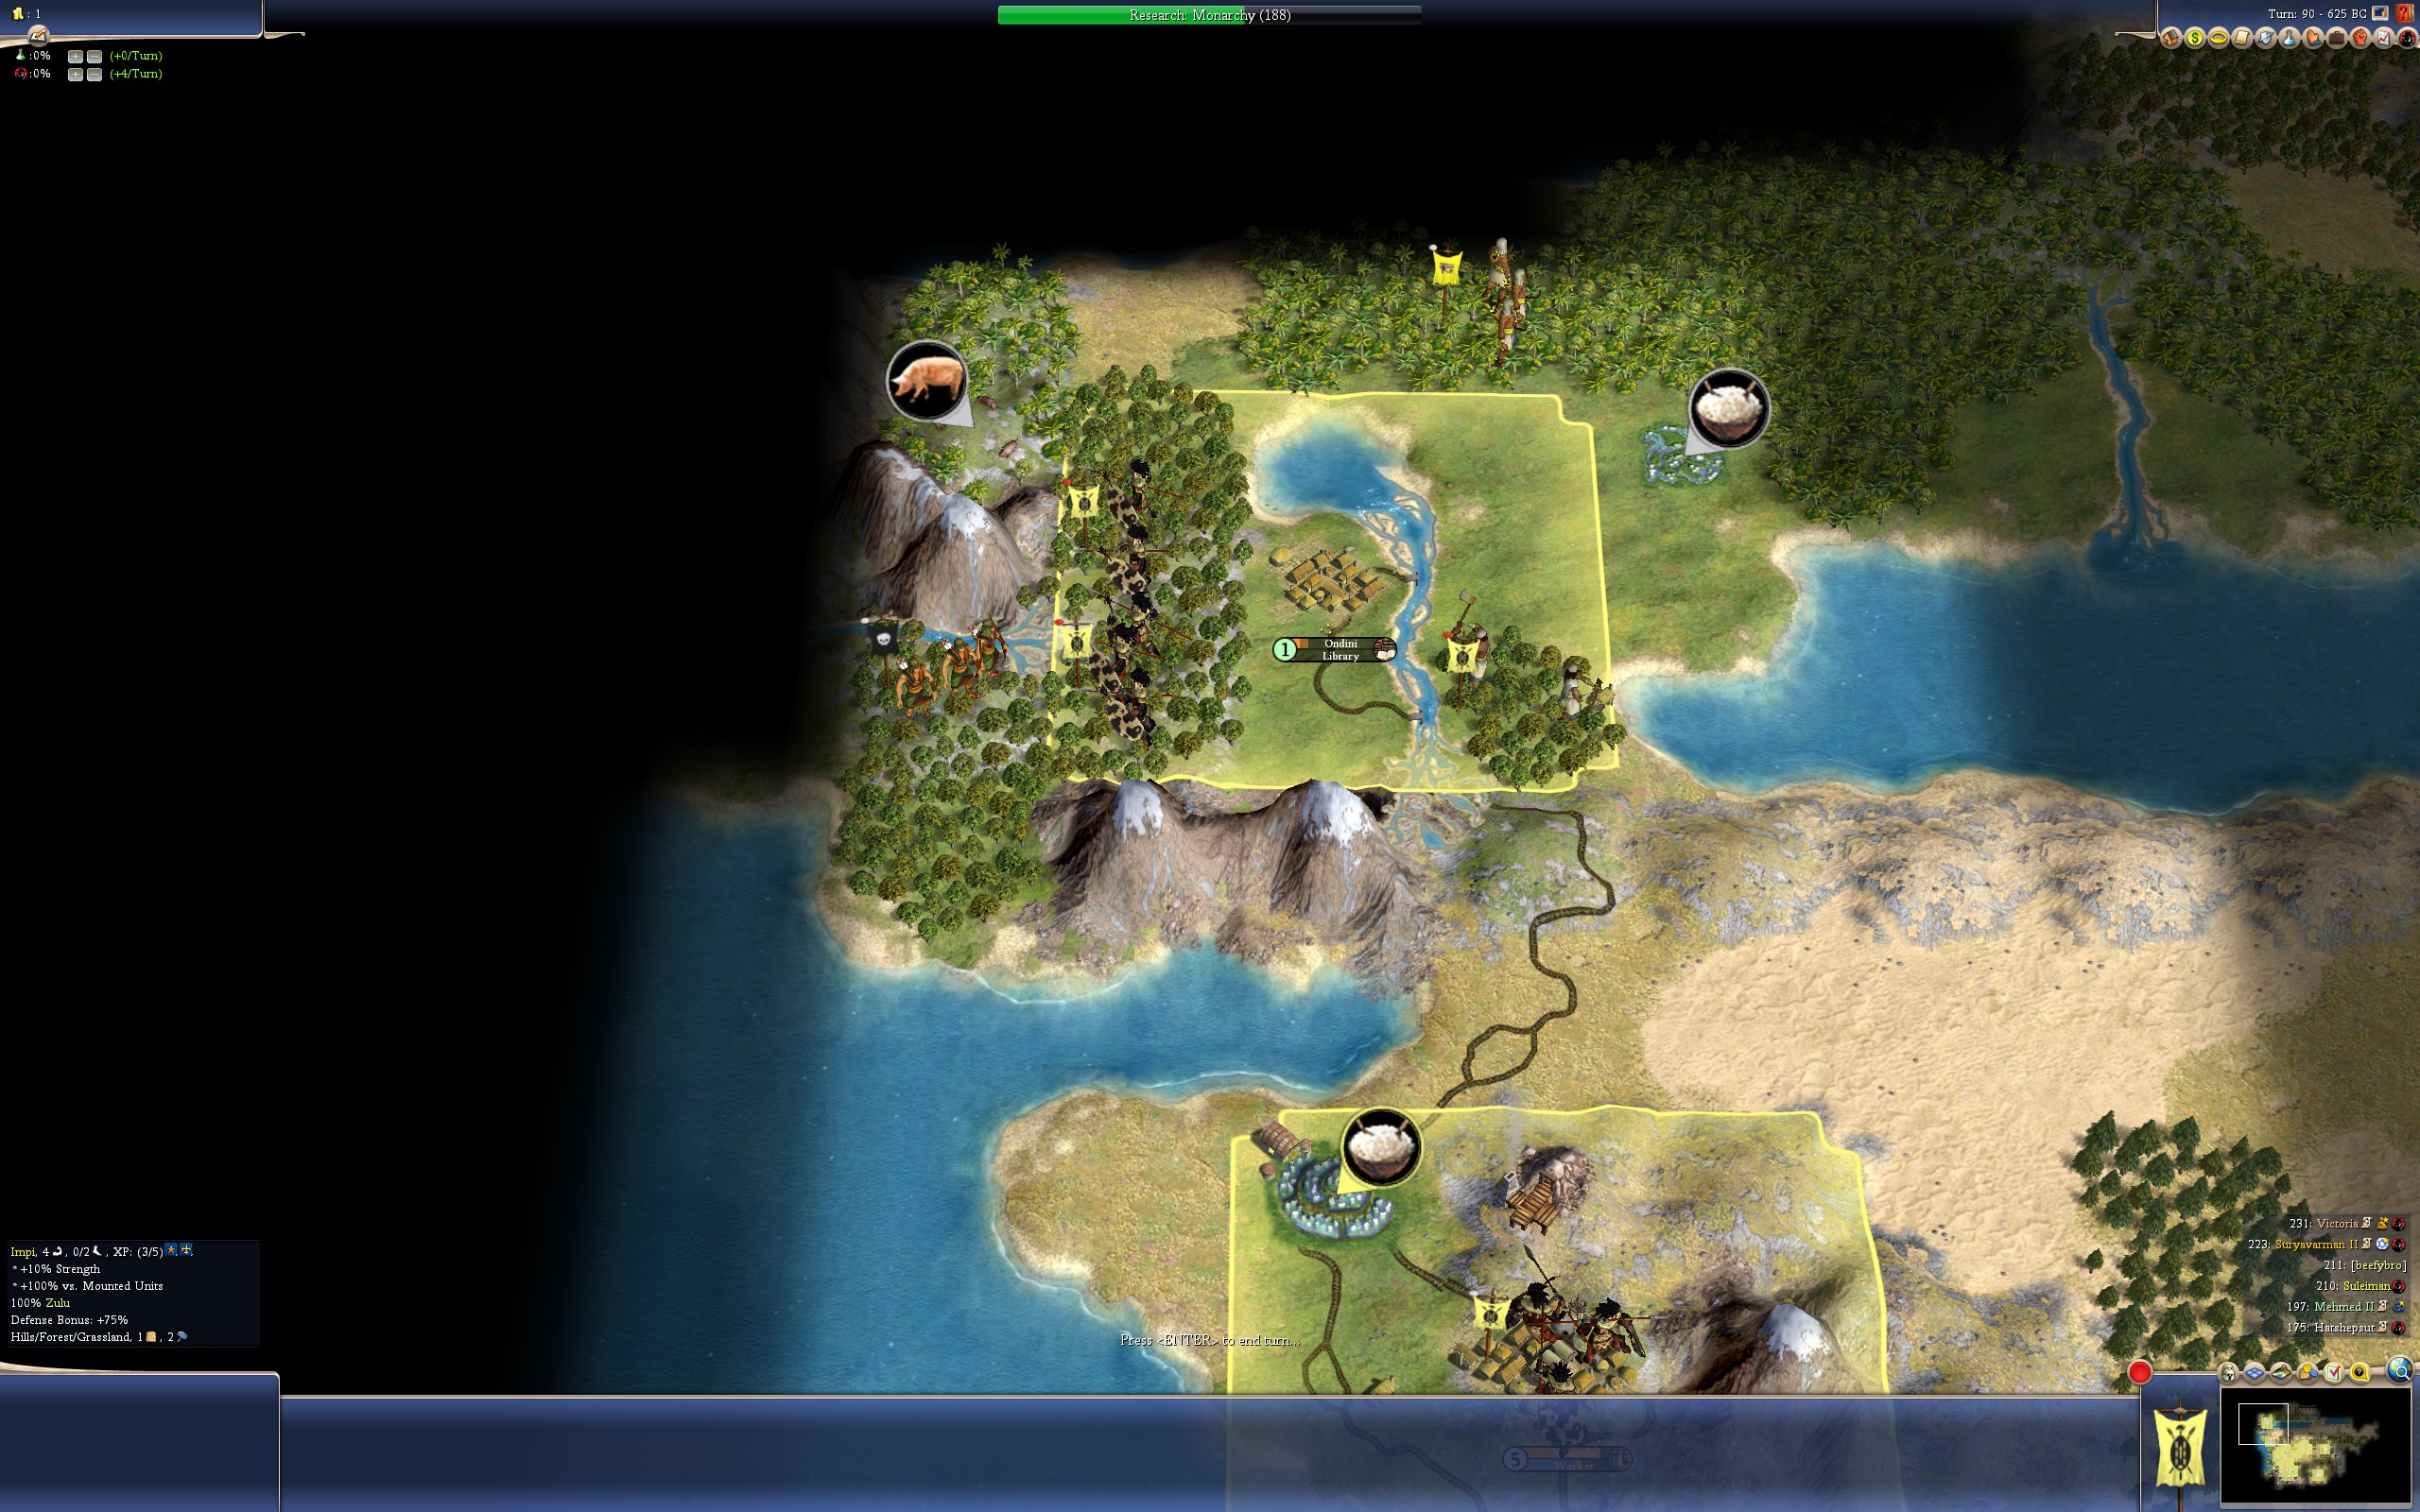
\includegraphics[width=1.0\textwidth]{59}

Just demonstrating another barb-control technique. I wall off the incoming barb archer from getting close
to my city by putting impis on forested hills, which are the best natural tile possible.

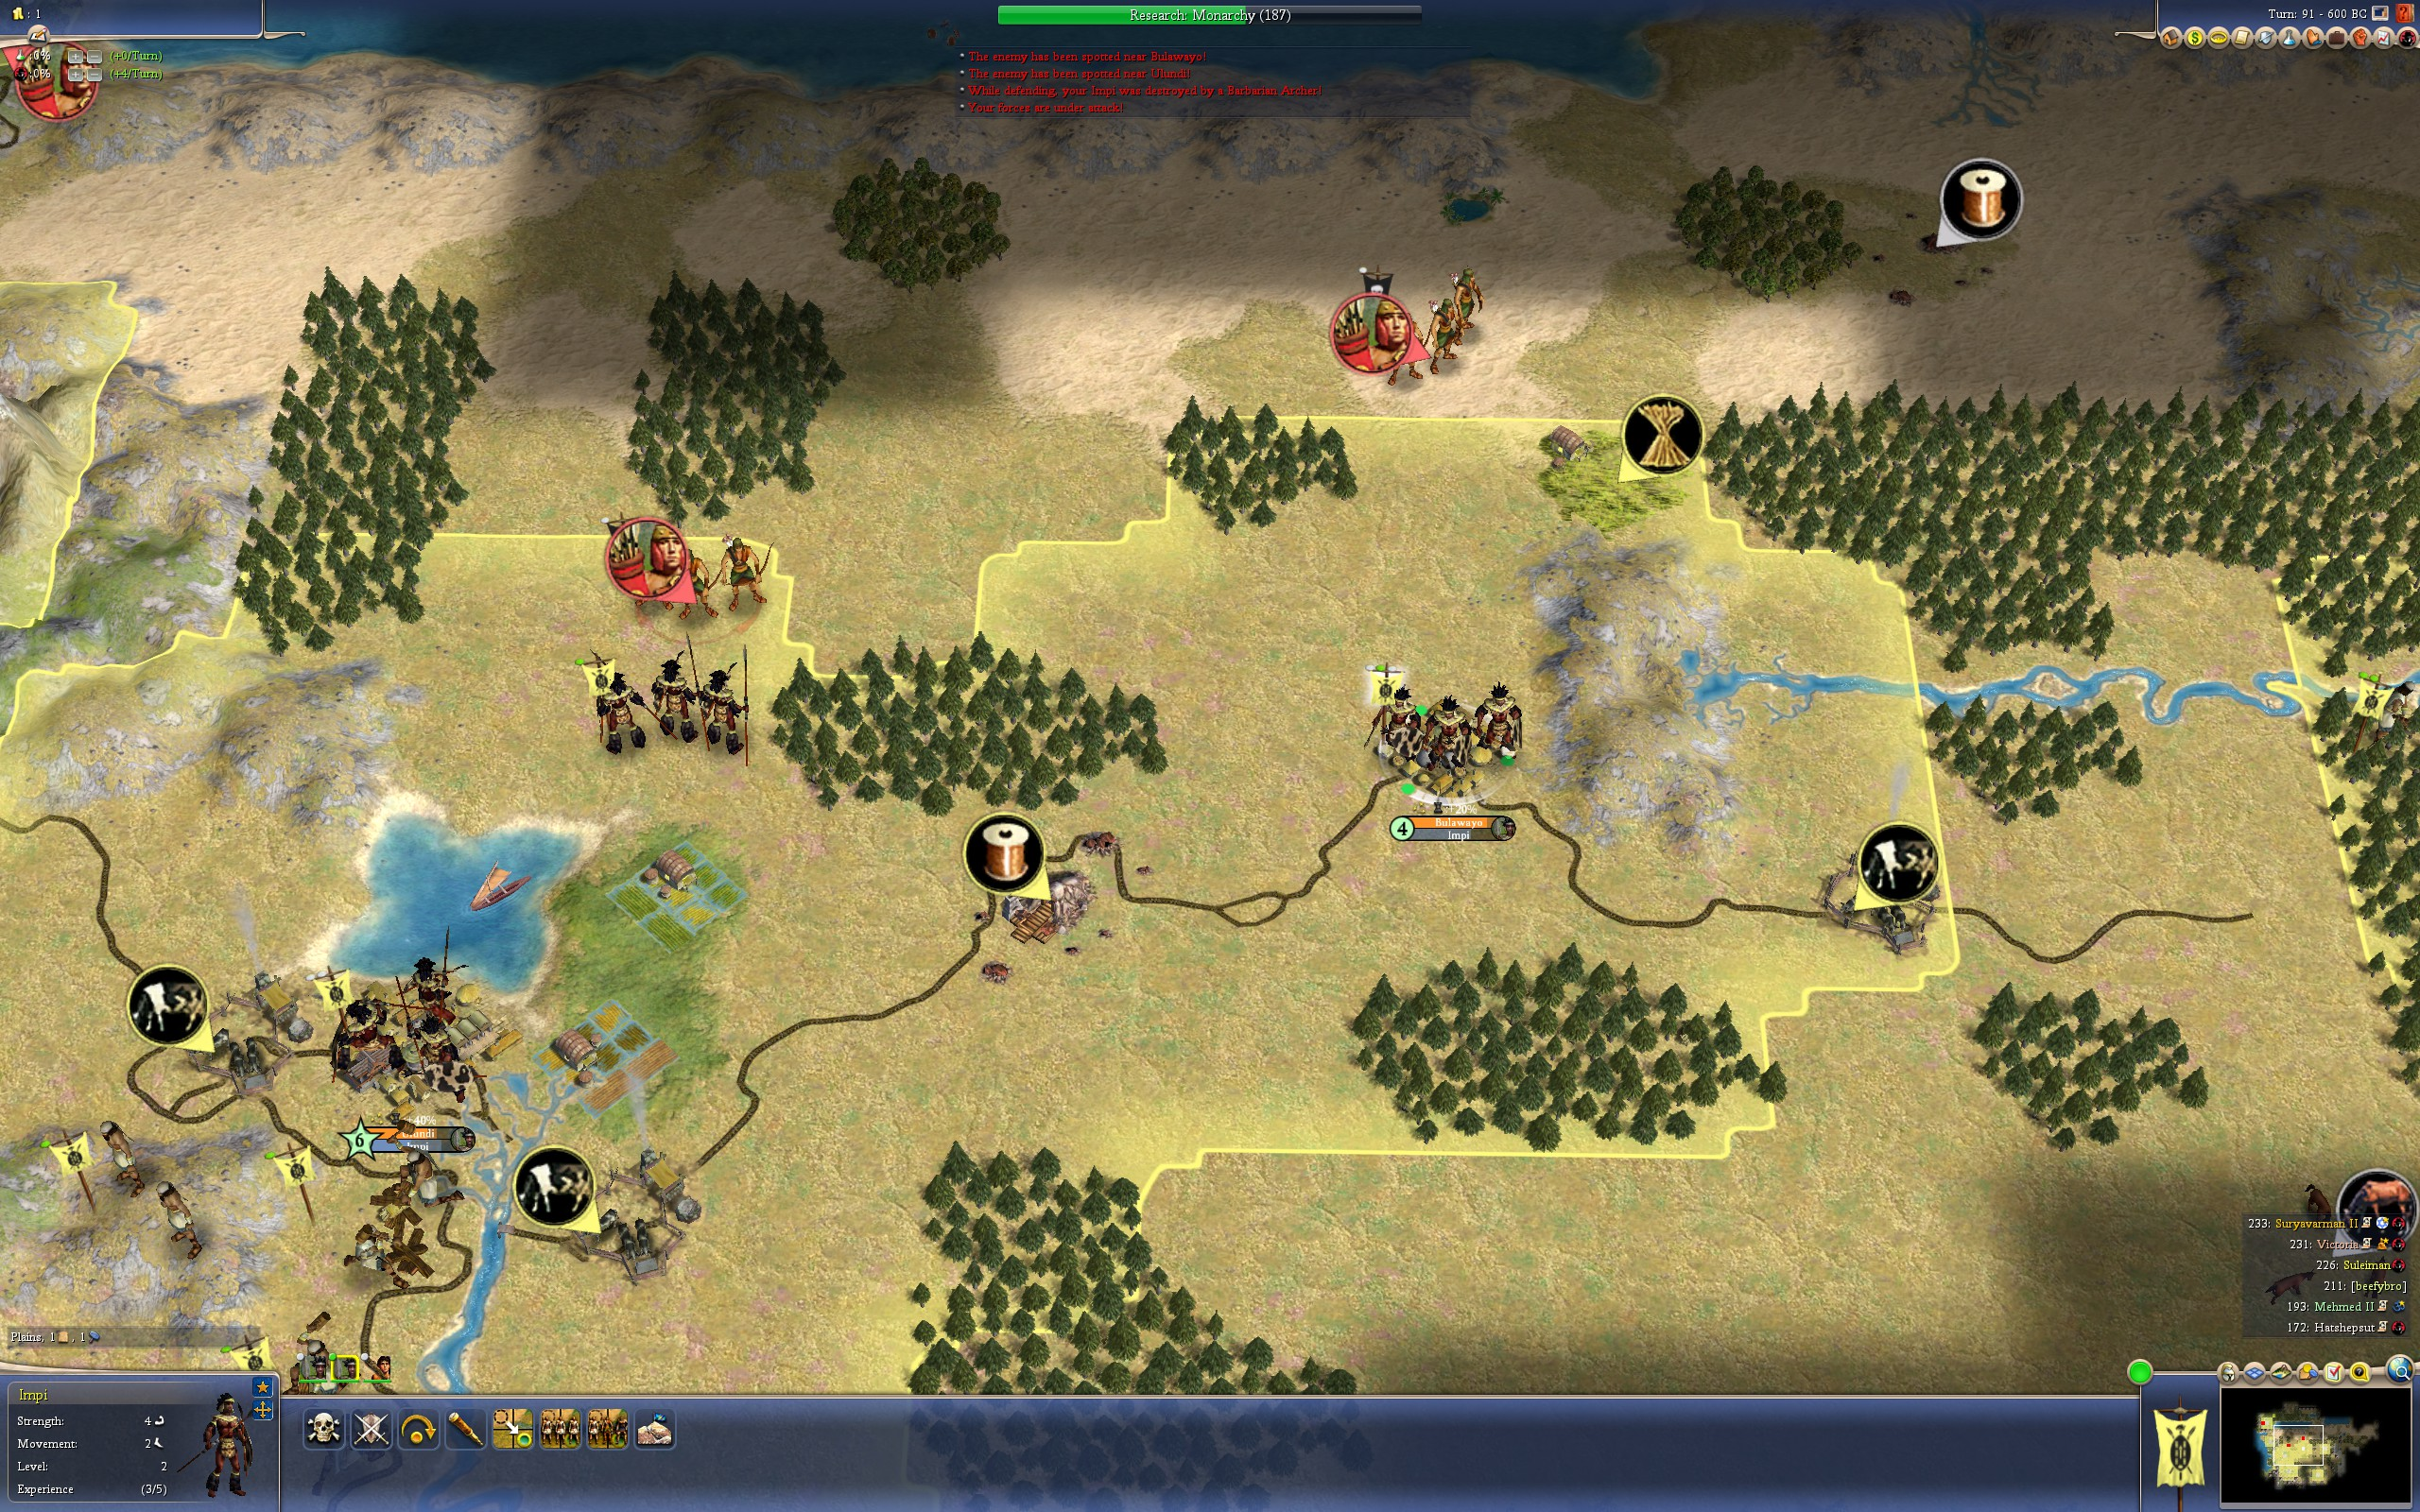
\includegraphics[width=1.0\textwidth]{60}

Barbs continue to flood in, my military city continues to pump impis non-stop.

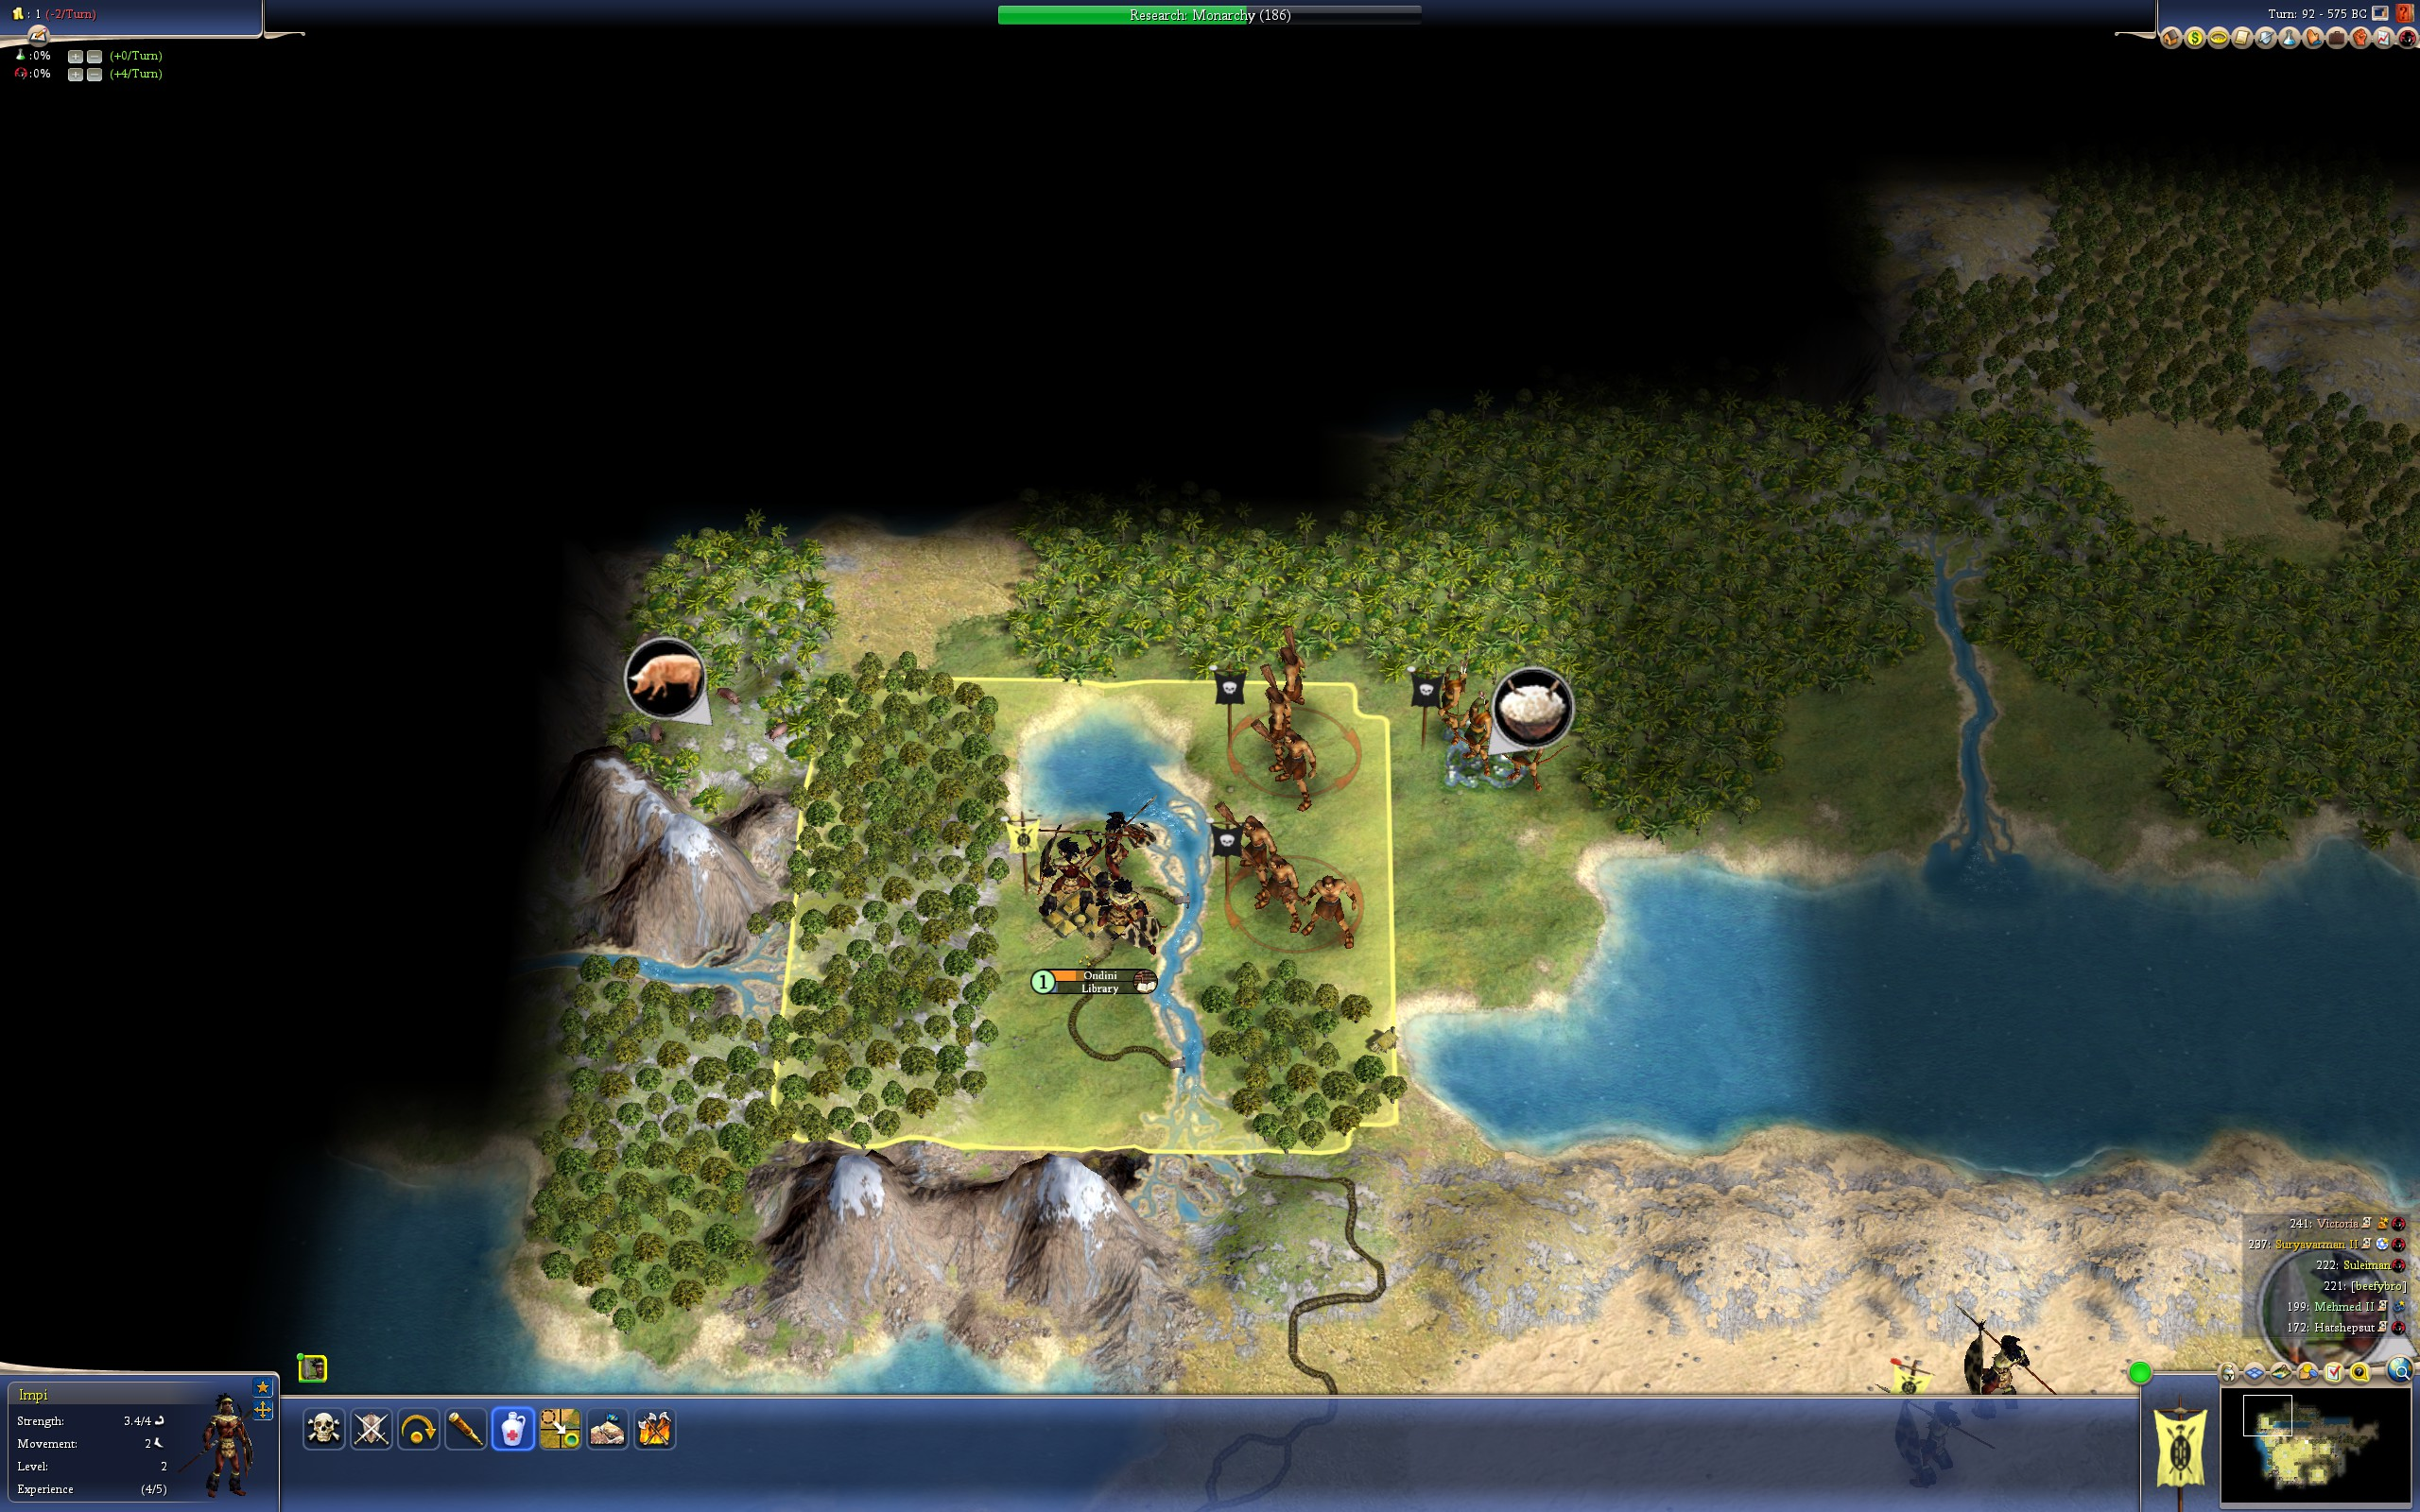
\includegraphics[width=1.0\textwidth]{62}

My economic situation has officially hit the fan. Non-stop rex and impi/worker spamming has taken a toll
and I'm now running a deficit even at 0\% science. It's officially time to panic and switch all cities off
of production tiles and onto commerce tiles.

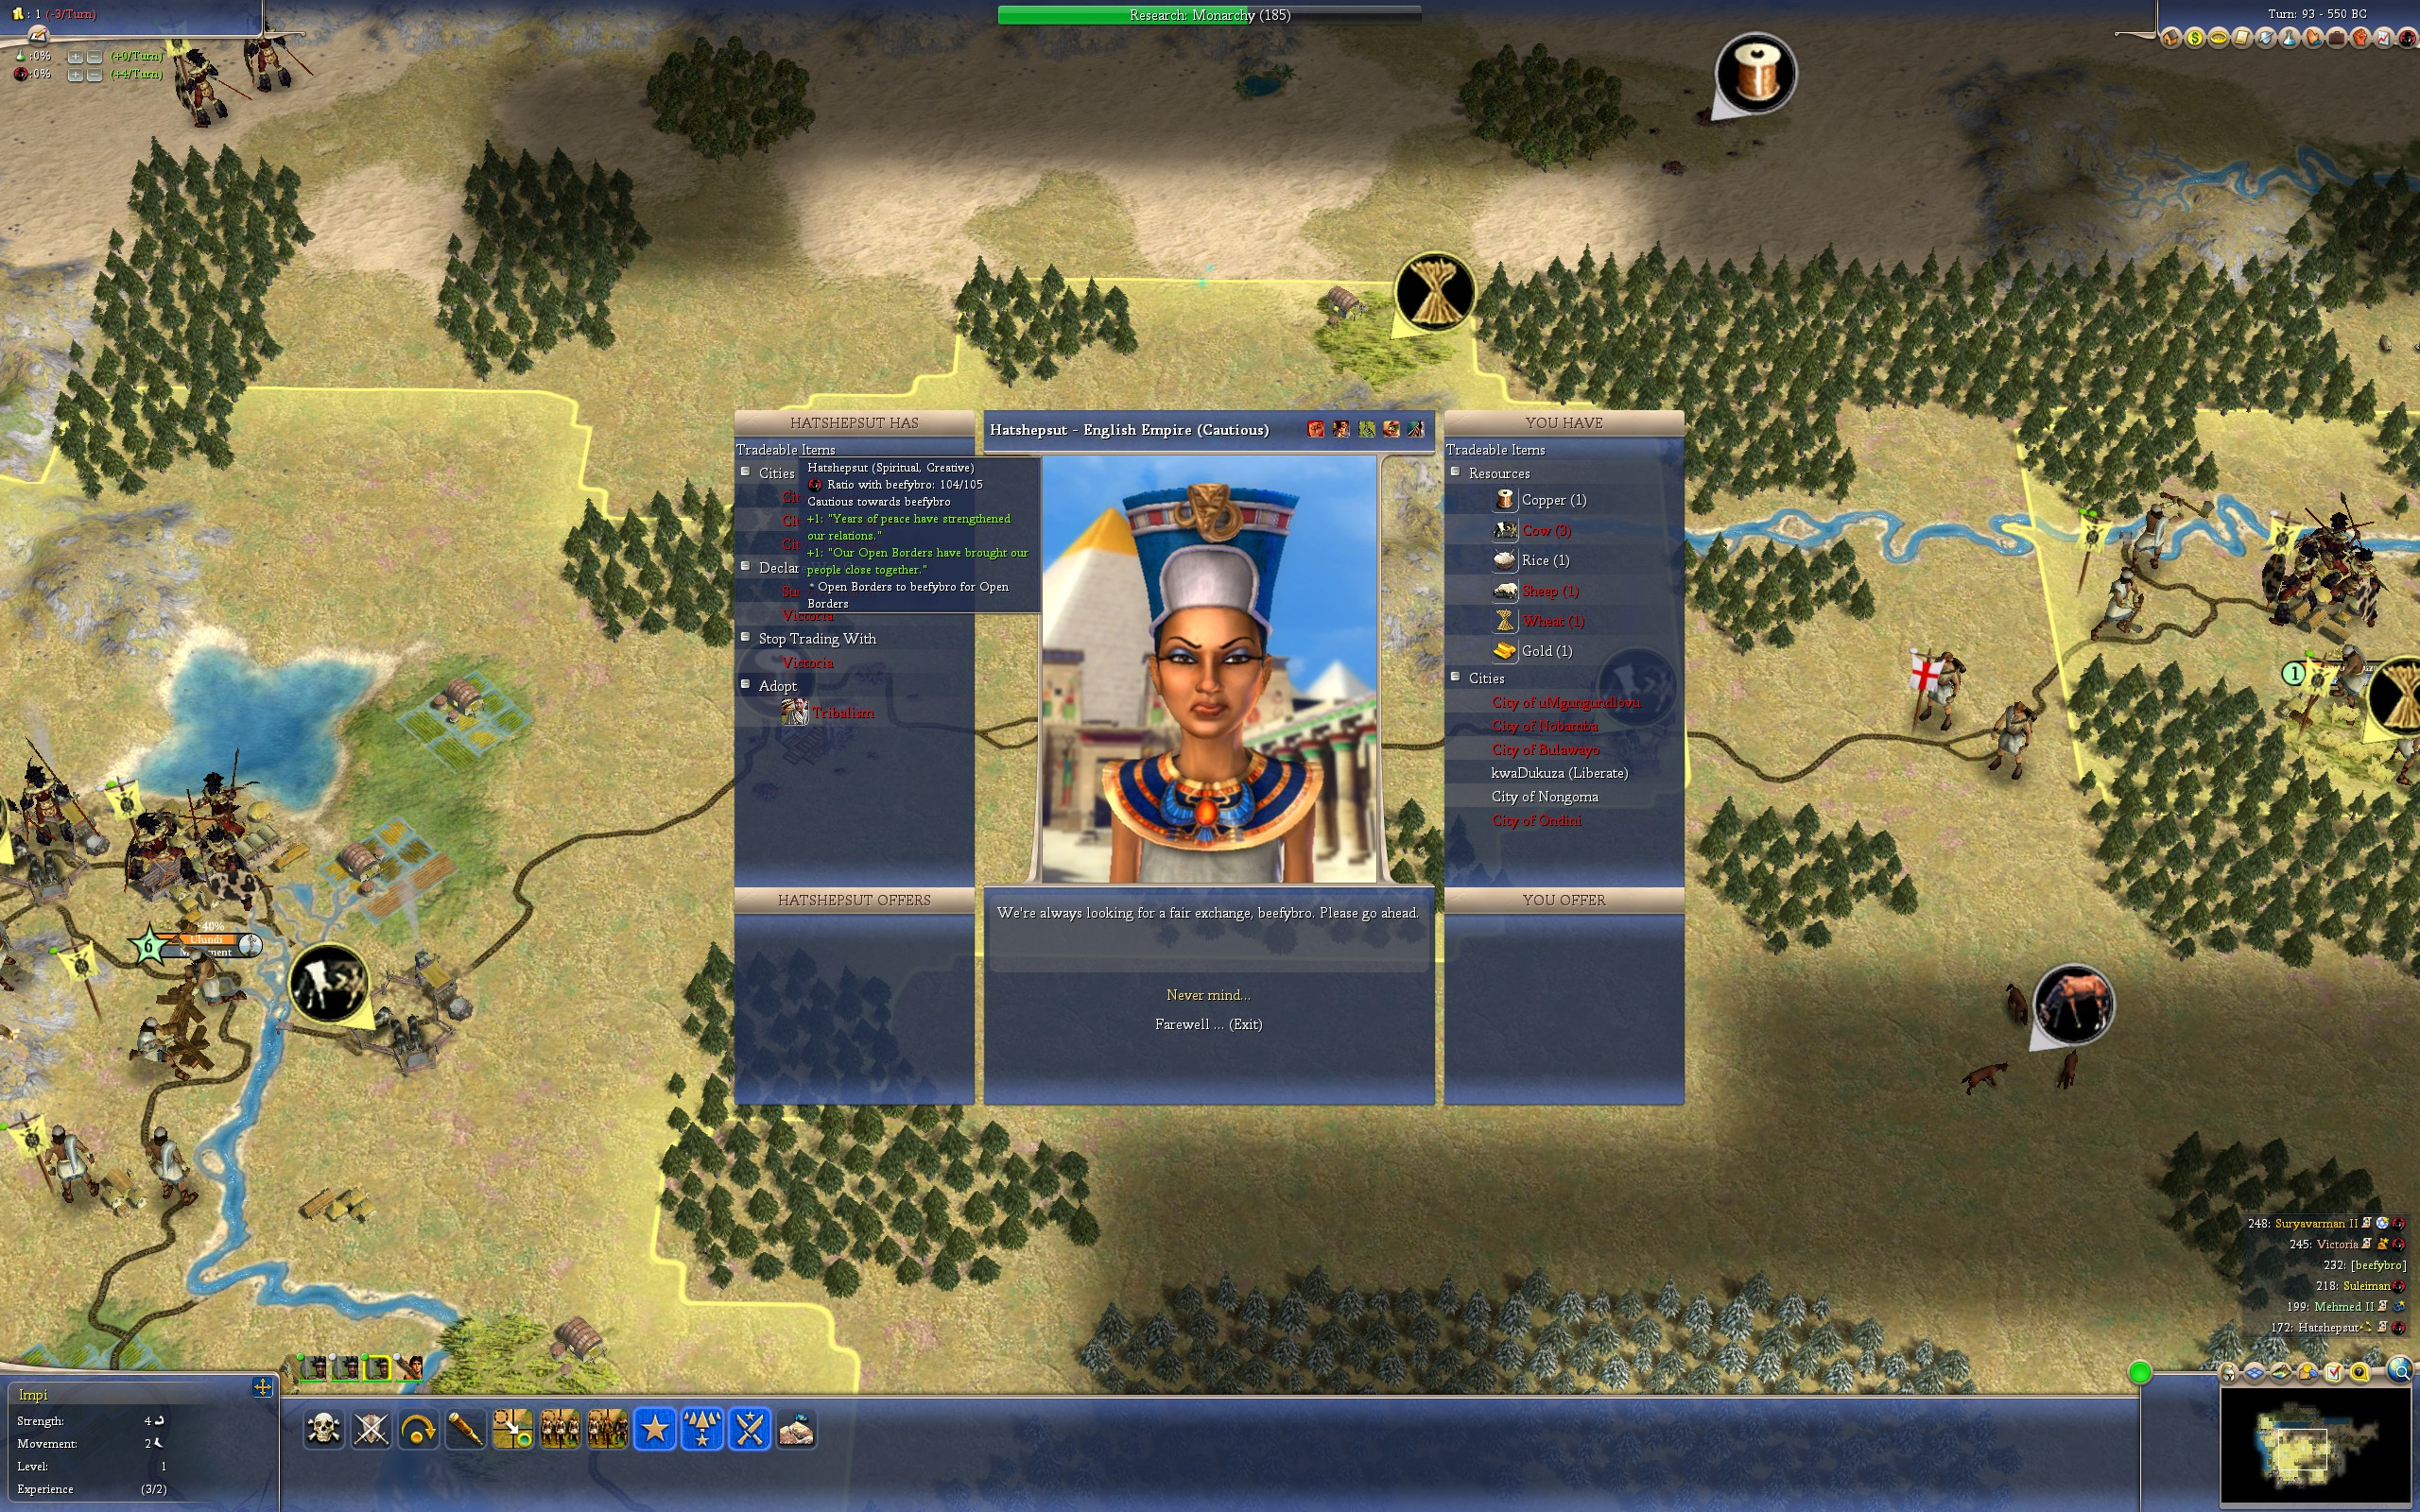
\includegraphics[width=1.0\textwidth]{63}

On the other hand, I have 7 cities and my neighbor has 4. This is dominant.

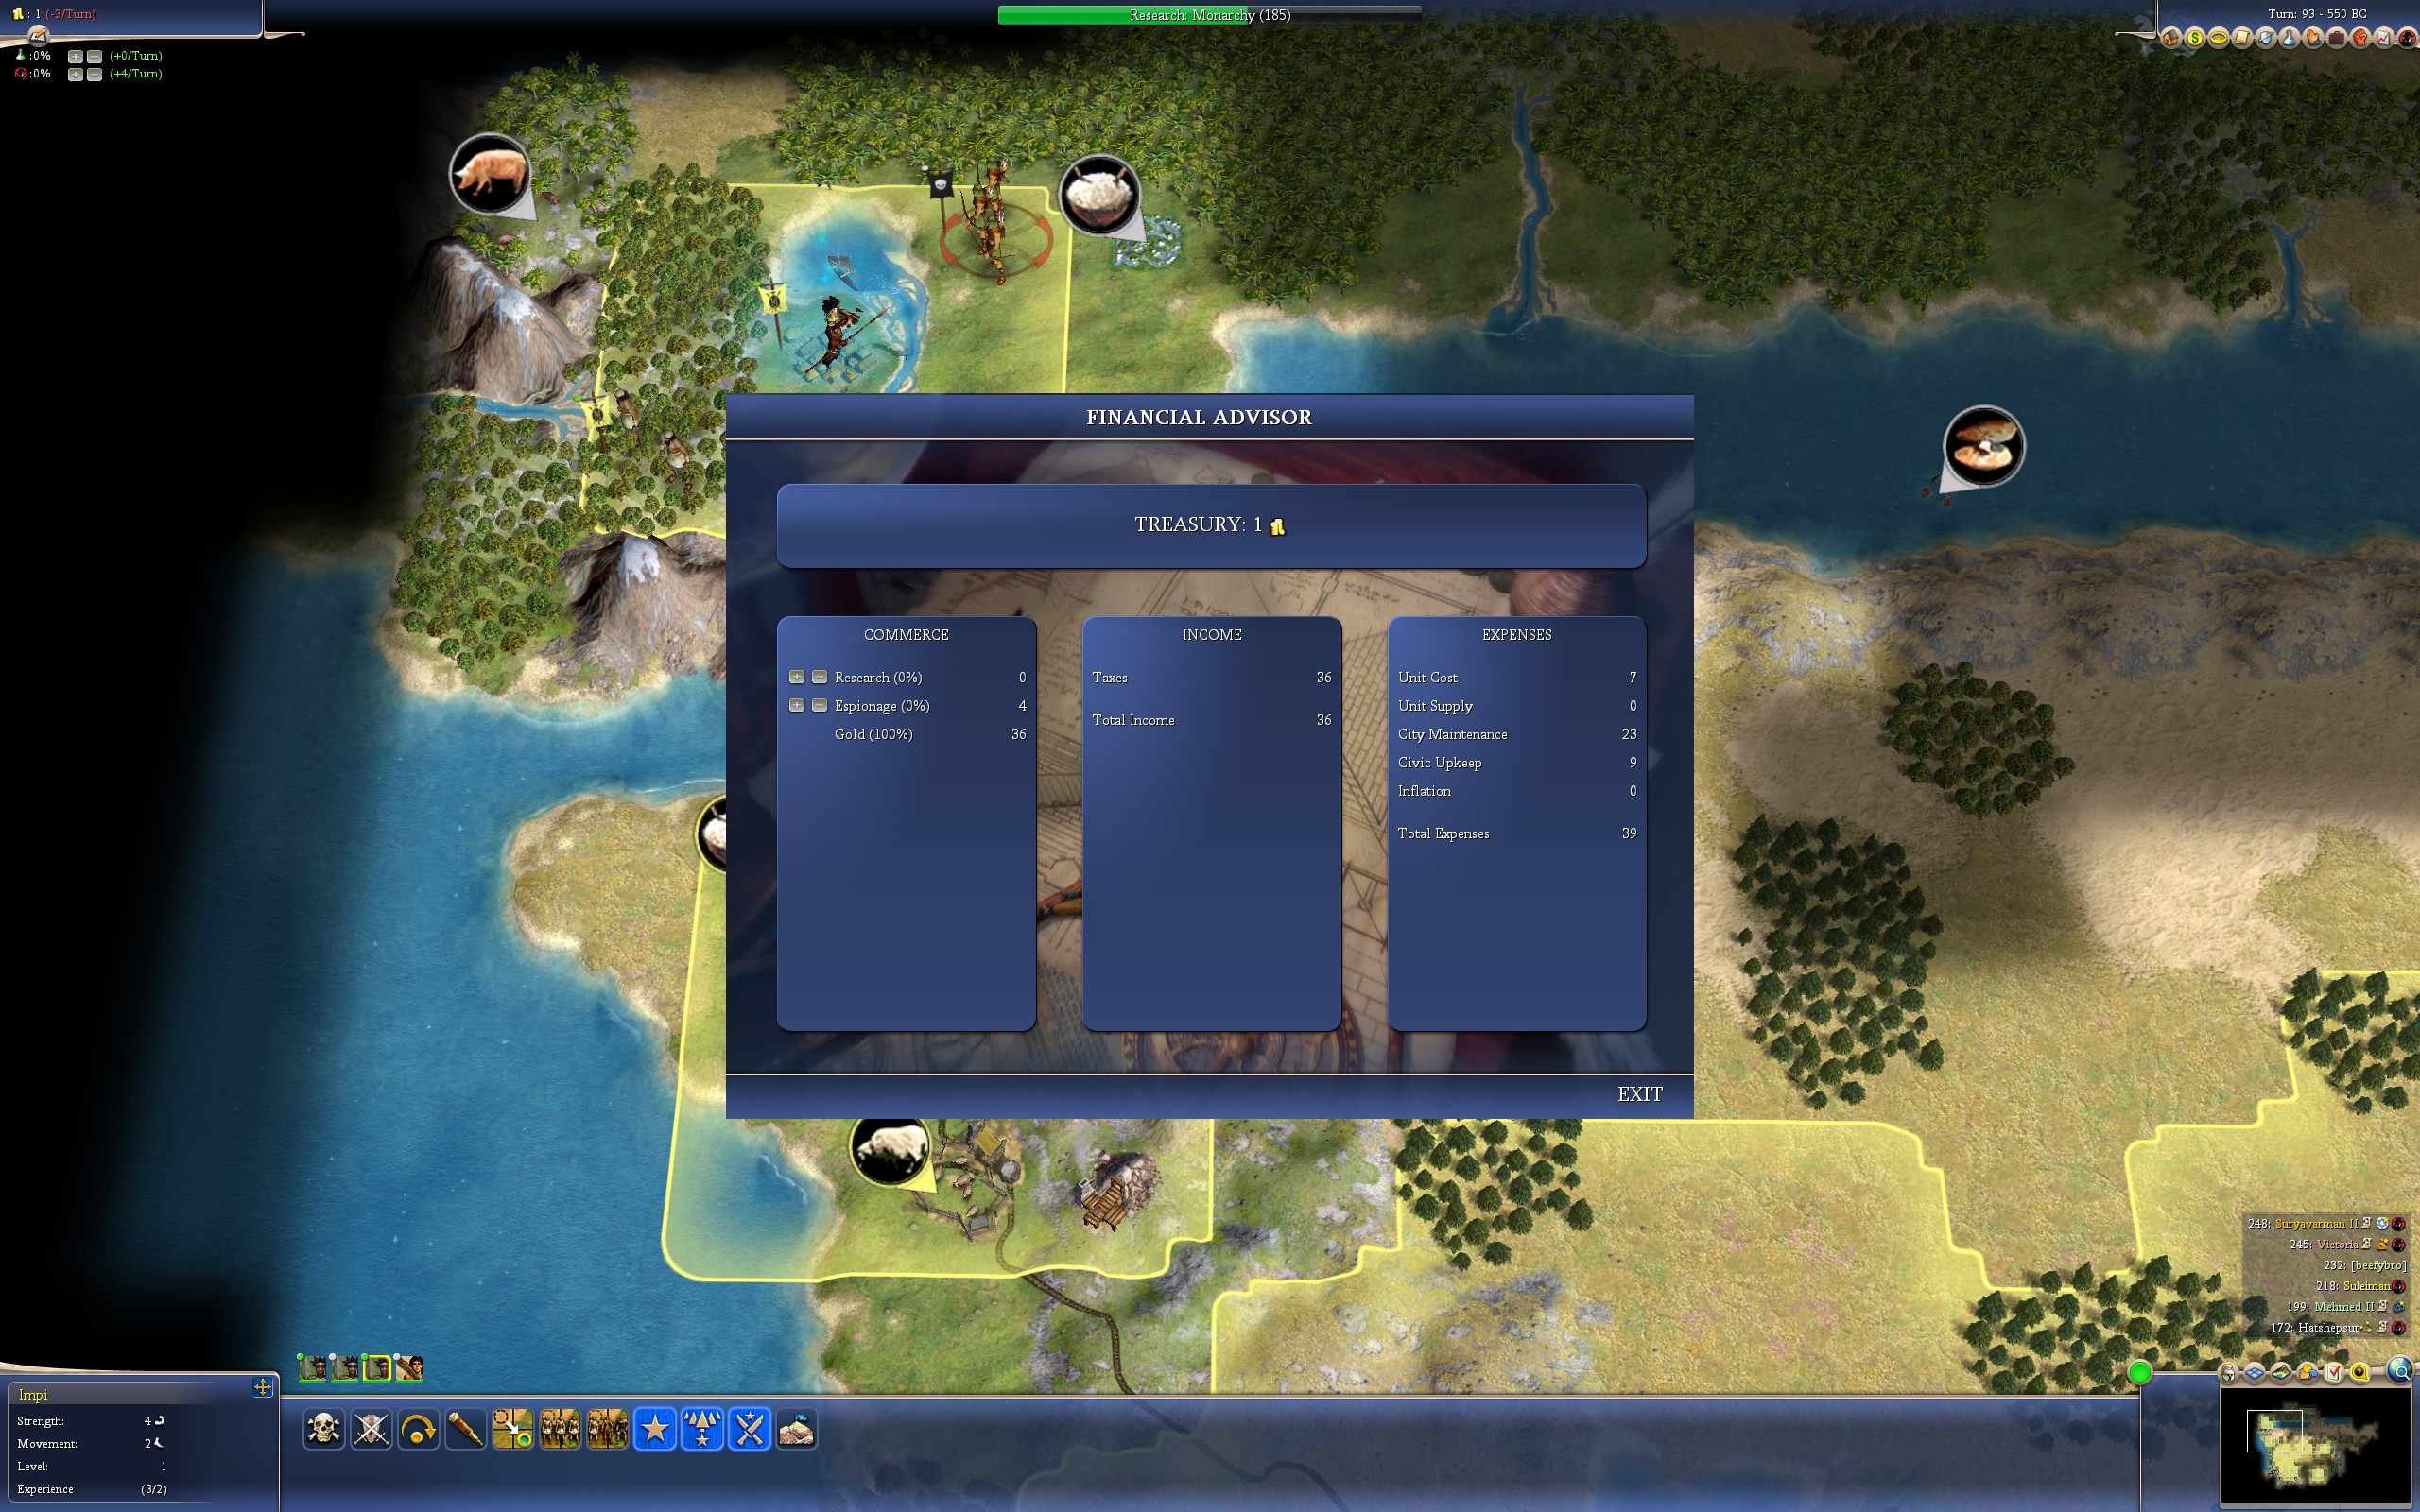
\includegraphics[width=1.0\textwidth]{64}

Here you can see my budget, with unit costs and especially city maintenance costing me massive
amounts of gold. This is what happens when you go crazy rexing.

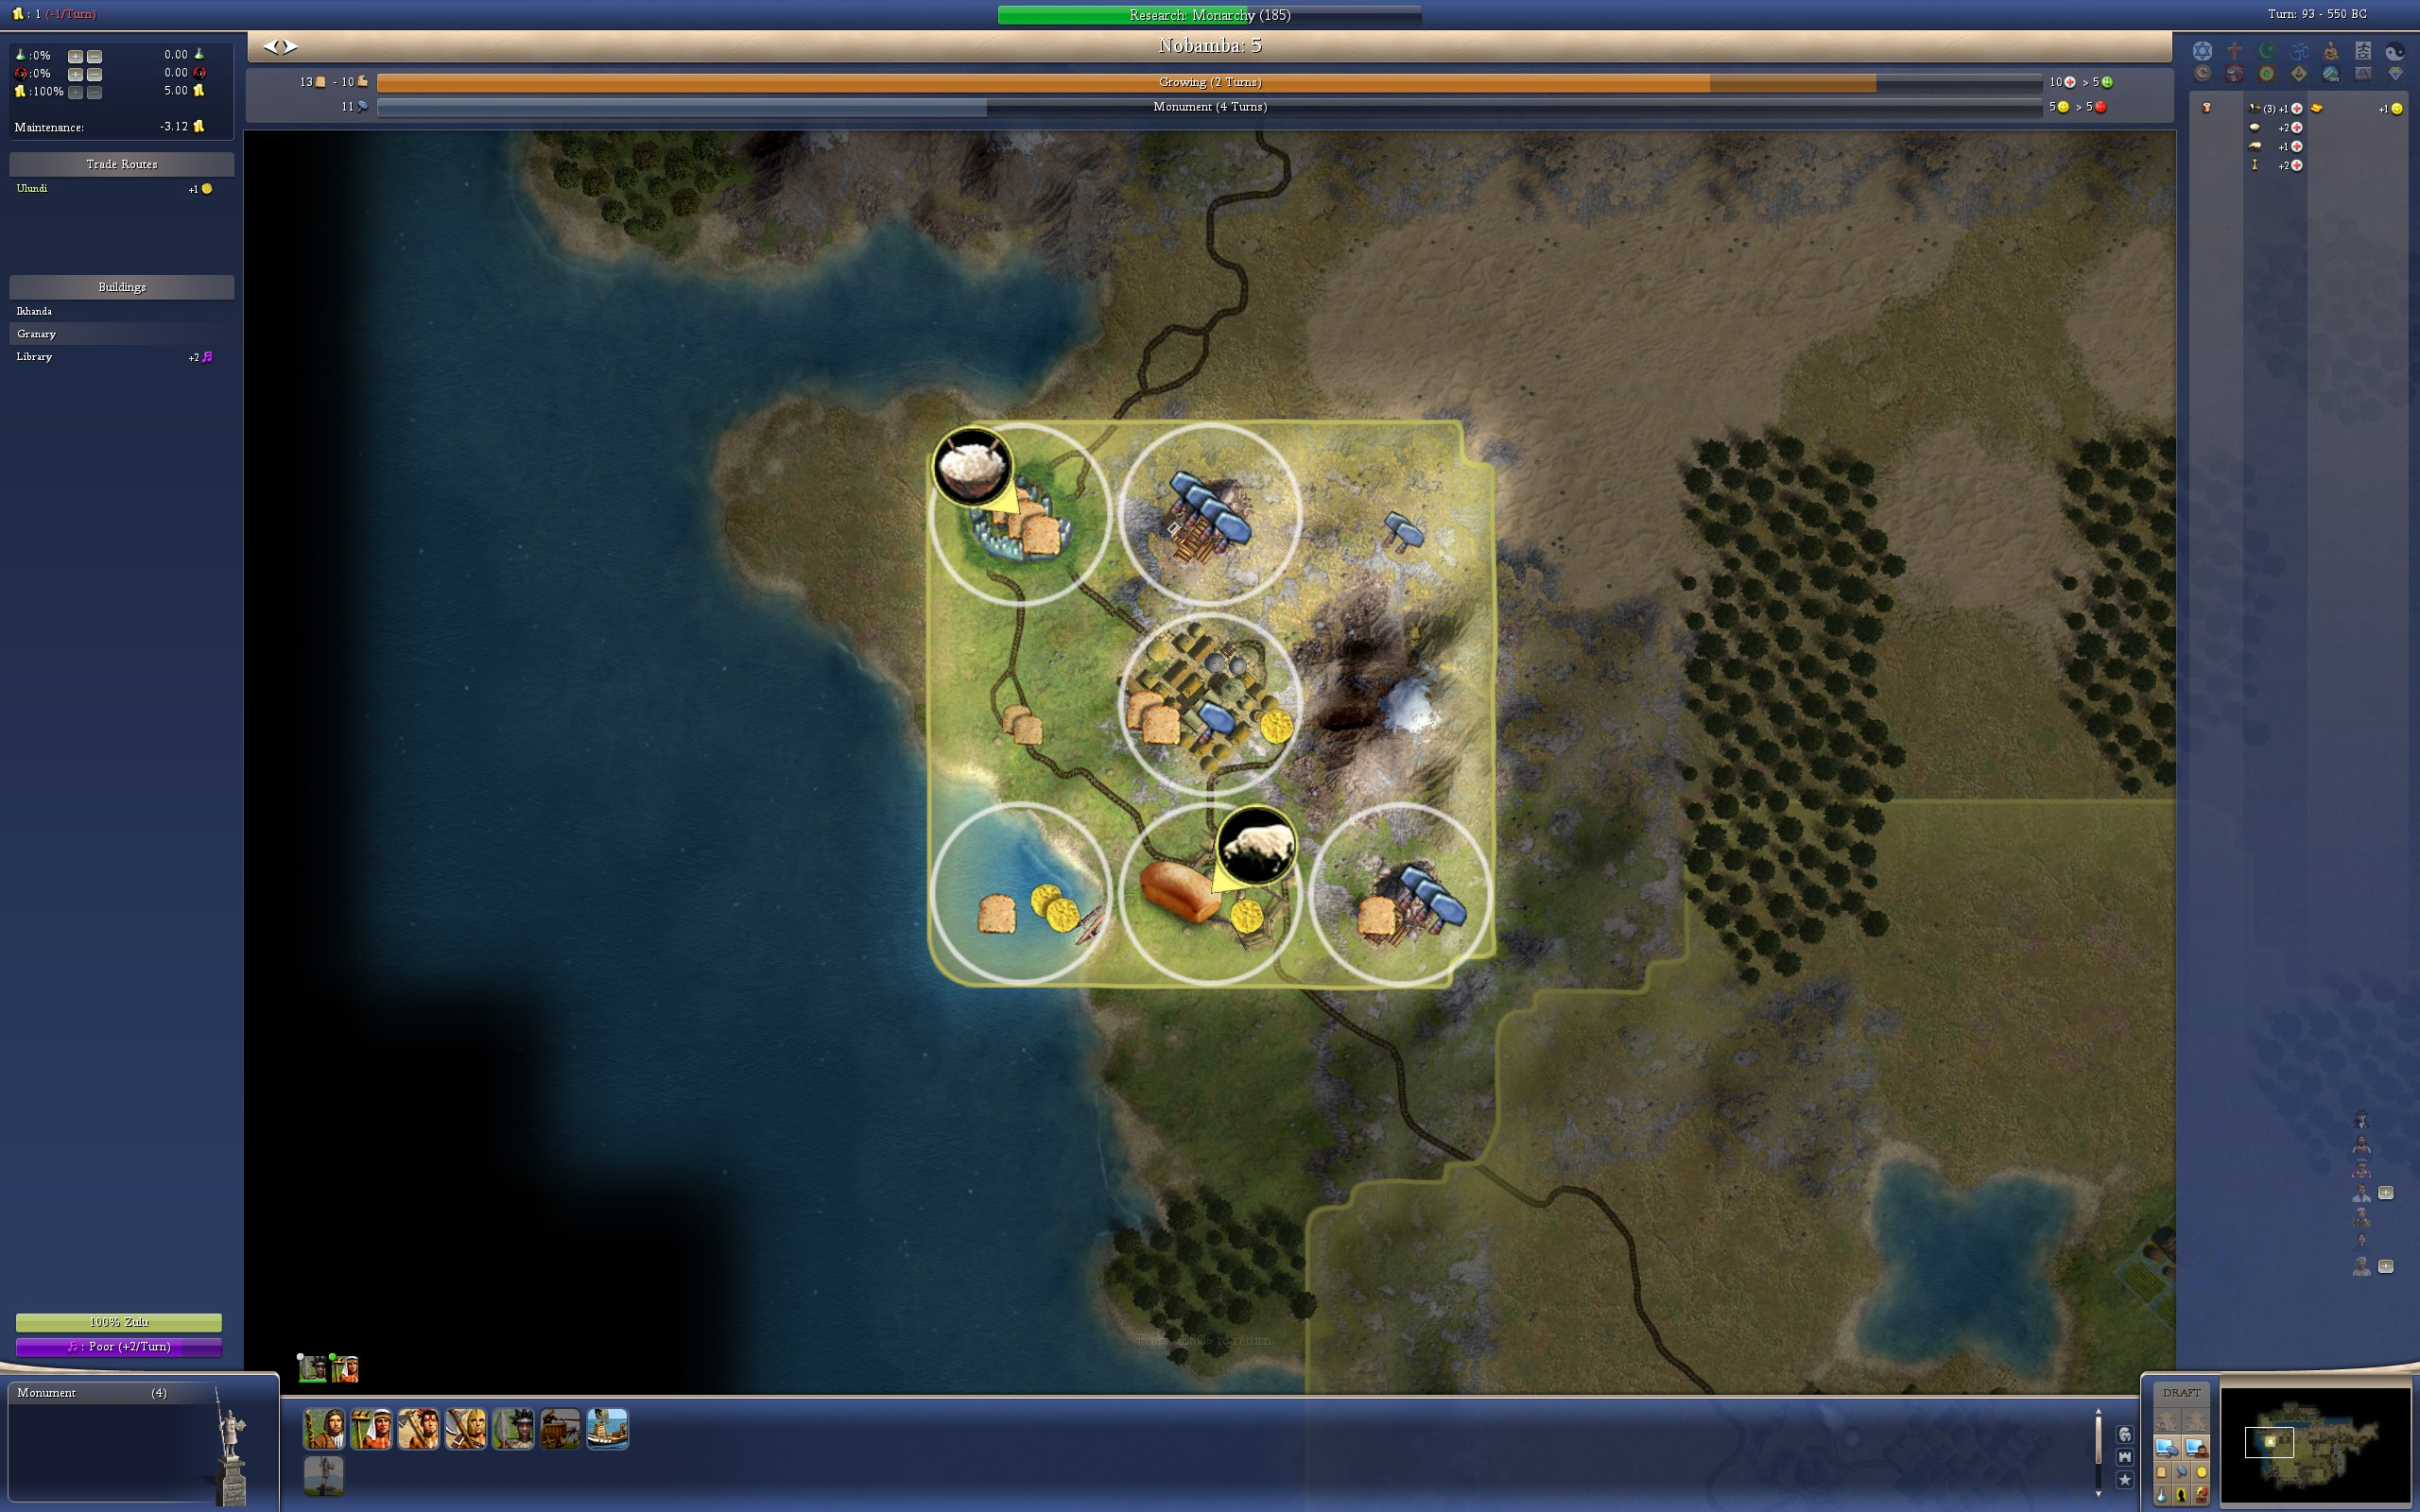
\includegraphics[width=1.0\textwidth]{66}

An example of me working suboptimal tiles in order to generate some commerce in order to prop-up my
economy. The coast tile (1 food, 2 commerce) sucks but at least gives a bit of commerce. I have to make
moves like this in all my cities to whatever extent possible.

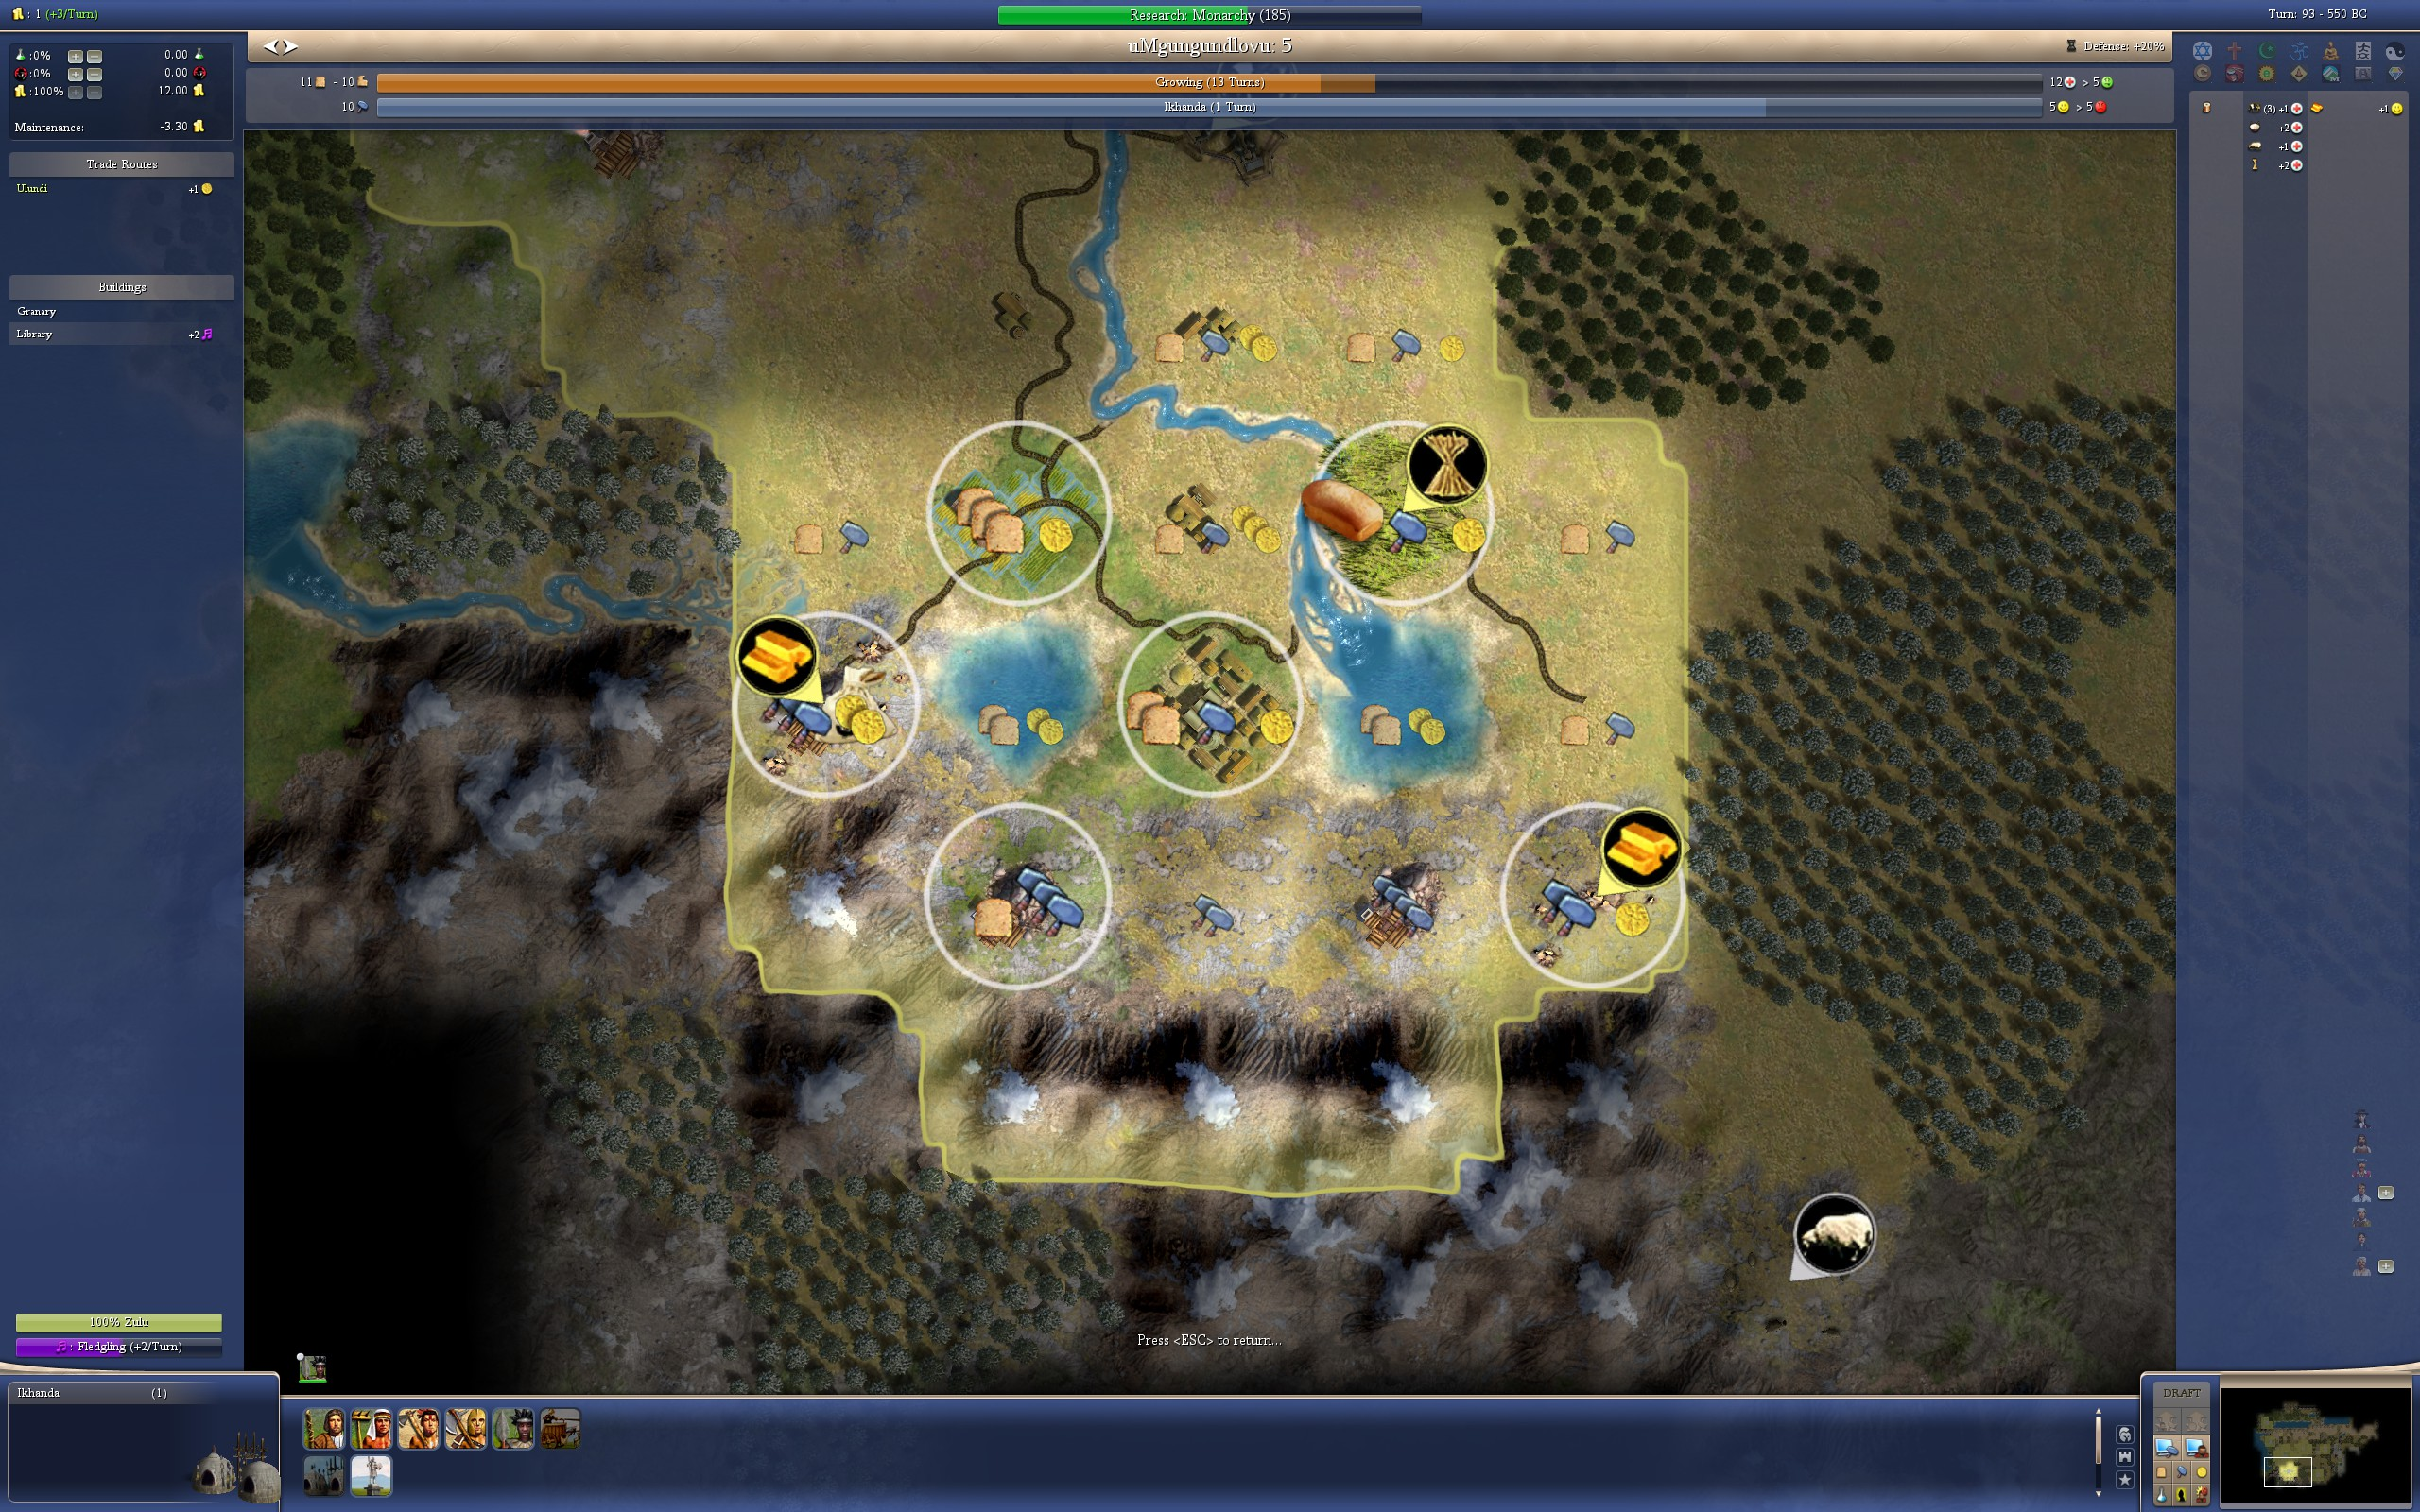
\includegraphics[width=1.0\textwidth]{68}

If it weren't for the massive amount of commerce from the gold mines, I might have thrown the game.

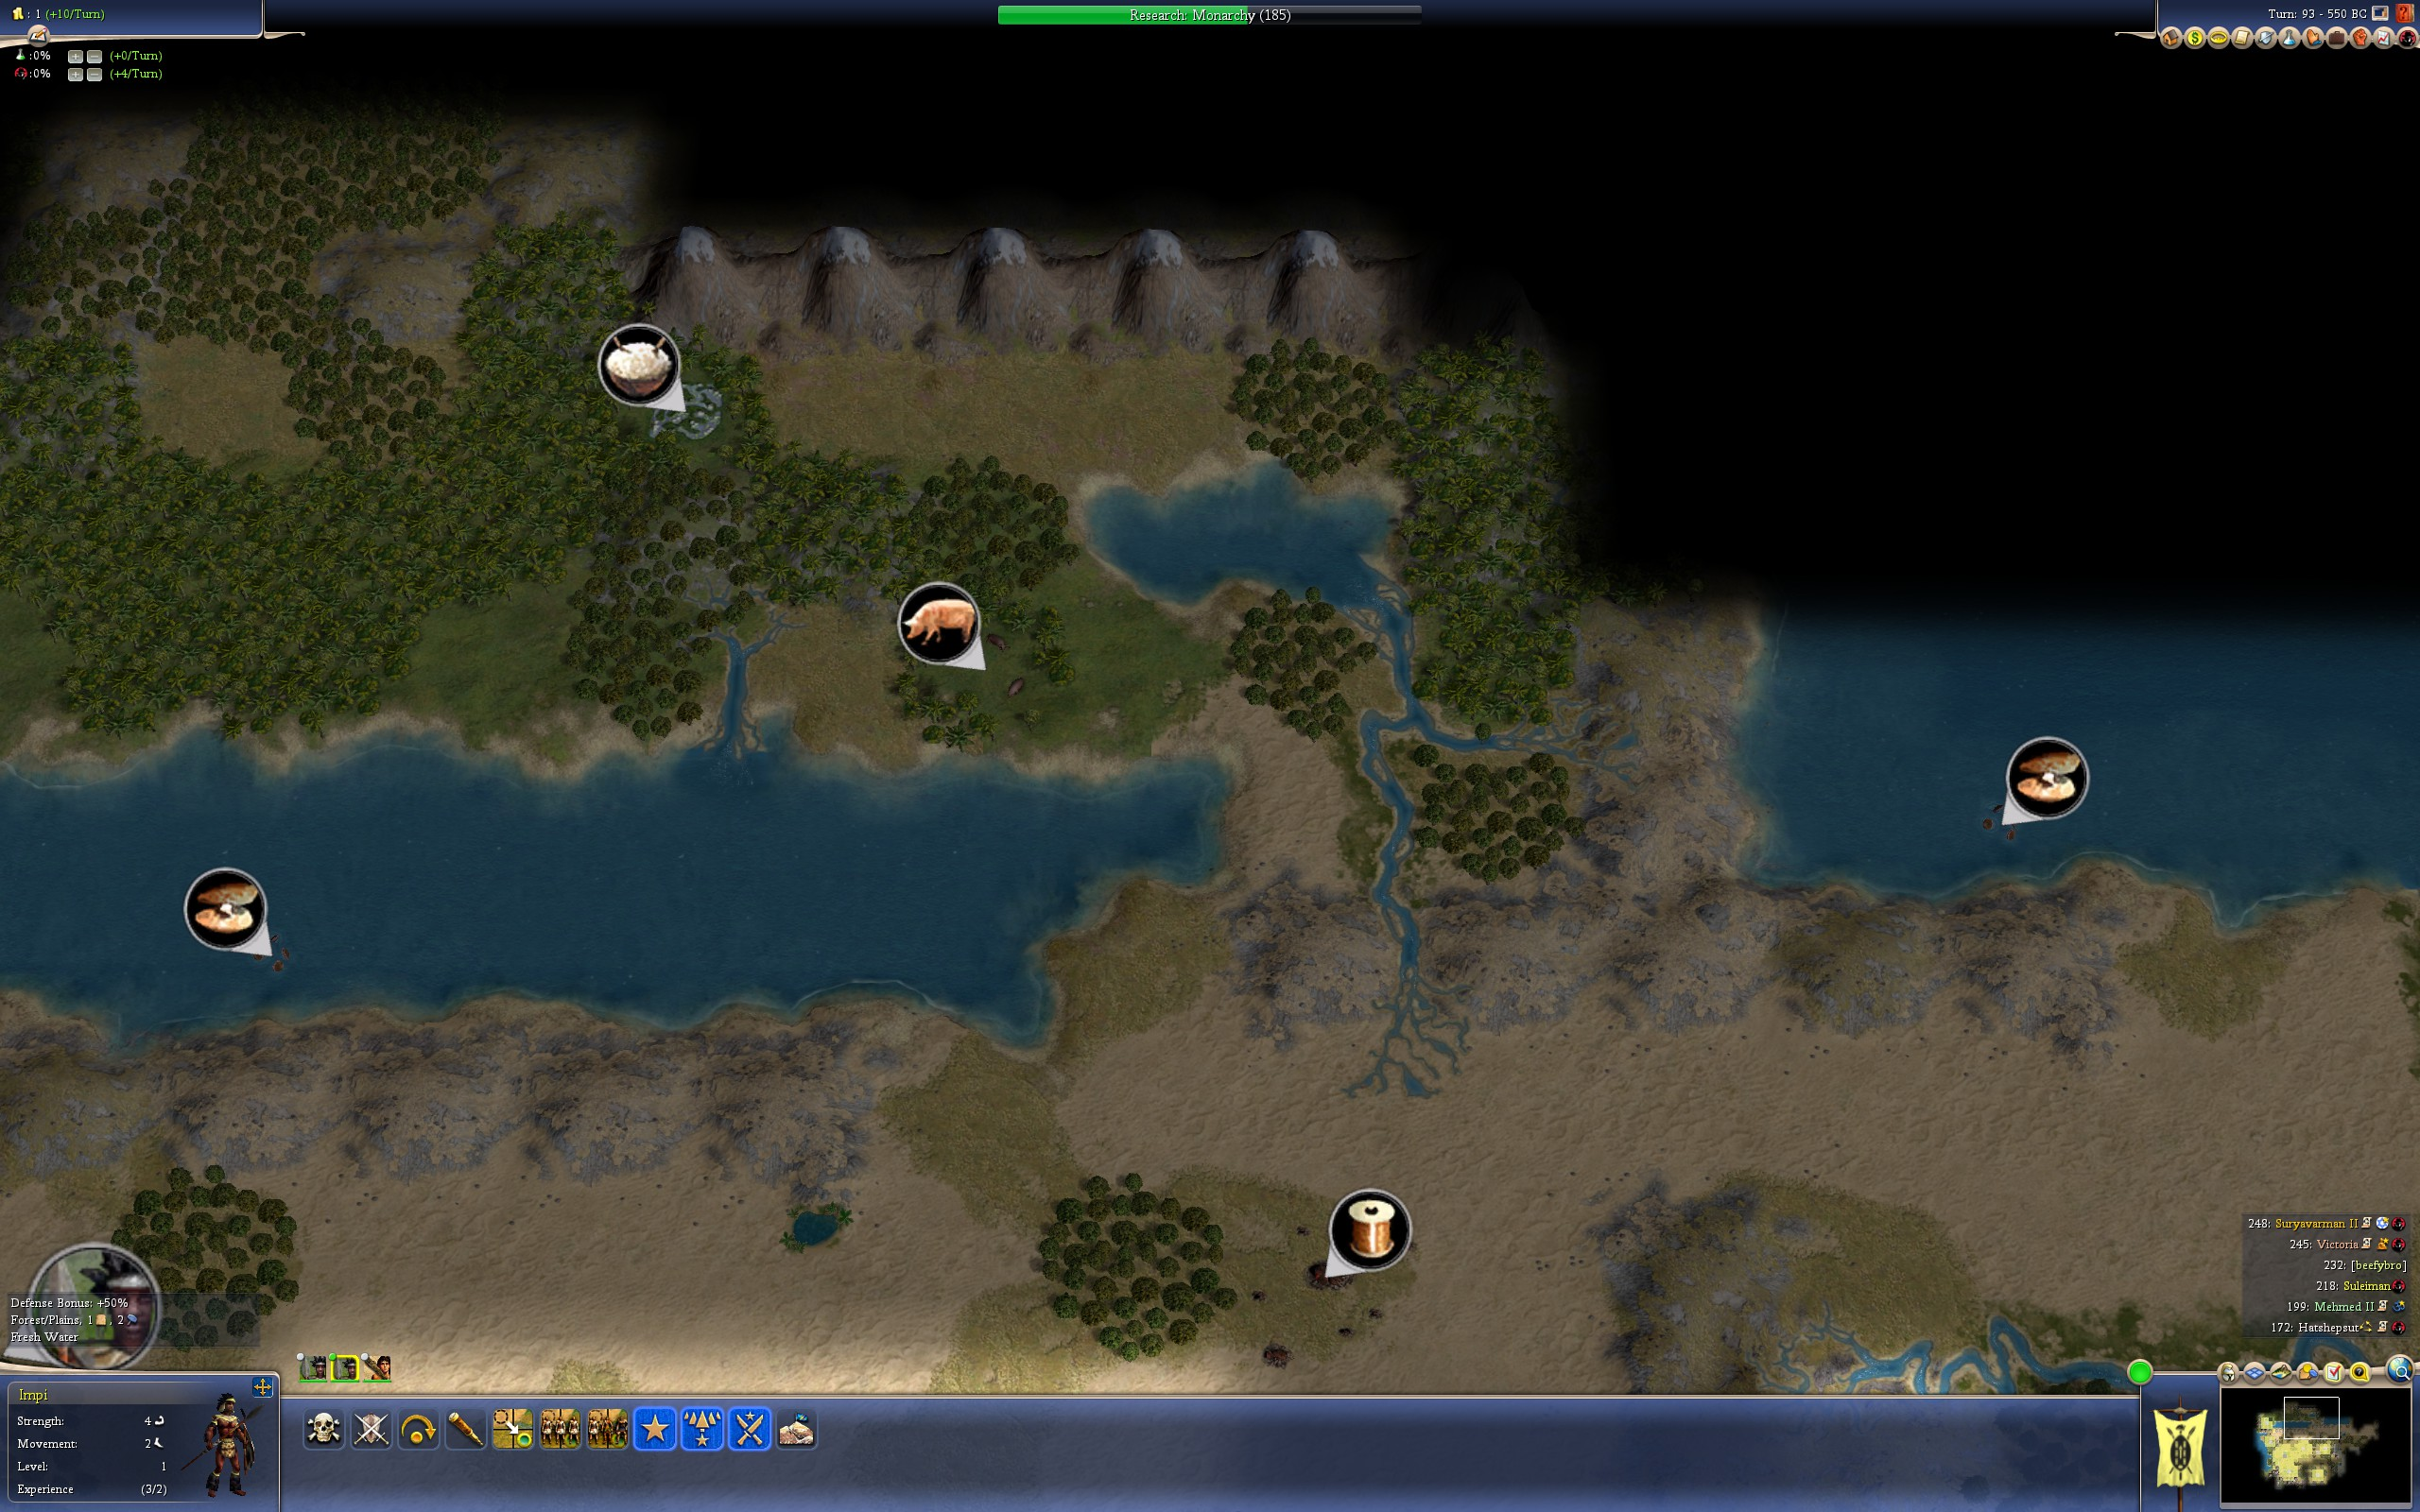
\includegraphics[width=1.0\textwidth]{70}

My next area of expansion to the north east. More juicy green tiles.

\includegraphics[width=1.0\textwidth]{71}

I'm back up to 20\% science with the changes to focus on commerce. Still bad, but progress.

\includegraphics[width=1.0\textwidth]{72}

Impis stationed on hills trying to bust fog and reduce the flow of barbs.

\includegraphics[width=1.0\textwidth]{75}

More impi fog busting. Don't forget that standing on a hill gives you +1 vision.

\includegraphics[width=1.0\textwidth]{76}

I'm so desperate for commerce that even my military city is getting in on the action by making
a couple cottages on a nearby river. I also make a library because I need to put hammers into
something that doesn't generate extra costs.

Also, notice that judiasm is spreading in my lands finally which will be very helpful.

\includegraphics[width=1.0\textwidth]{78}

I still don't have sailing, so I need to make roads to Hatty to get the connection.

\includegraphics[width=1.0\textwidth]{80}

With routes to Hatty, I'm up to 30\% beakers and the crisis is over.

\includegraphics[width=1.0\textwidth]{81}

Monarchy is finally done and I can switch into the excellent Hereditary Rule. I would normally take this opportunity
to also switch to slavery for zero additional cost, but slavery is medium upkeep and tribalism is low upkeep and
every gold piece matters due to my overexpansion, so I'll pass on slavery for now.

\includegraphics[width=1.0\textwidth]{82}

With Monarchy done, it's time for a new tech. With my overexpanded situation, I have to go for Code of Laws (CoL)
in order to get courthouses even though it's an expensive tech. At my current rate, it will take 18 turns. I'll
have to limp along until then with no new cities going down.

\includegraphics[width=1.0\textwidth]{84}

Now that it's getting closer to 0AD, there's an increasing risk of barb axemen spawning. Those would destroy
my impi defenders, so I've mostly switched to axemen and making sure border cities have at least one axeman.

\includegraphics[width=1.0\textwidth]{85}

Starting to claim the far northeast territory. This city maybe could have waited until CoL was done. I'm now running
a significant deficit at 30\% beakers.

\includegraphics[width=1.0\textwidth]{86}

A view of the world as we hit 0AD. I have a total of eight cities, which is an excellent rex effort. The three golds
(I got crazy lucky and spawned a gold in Nabamba) and the -20\% maintenance from my super-barracks allowed me to
achieve this.

\includegraphics[width=1.0\textwidth]{87}

I start sending surplus axemen to nearby barb cites. A city-raid axeman is pretty dominant over a barb archer in
a city. Also, the city capture will give me a nice gold boost to help get me to CoL.

\includegraphics[width=1.0\textwidth]{88}

A look at my far-east river city. The two food nodes and river make this an excellent commerce city. Growth will
eventually stall due to lack of food because every tile besides the bonus tile comes with a -1 food deficit.
Judaism has finally spread to my civ, giving me useful things to build without adding to the deficit.

\includegraphics[width=1.0\textwidth]{89}

I've switched my military city over to making missionaries to spread judaism as fast as possible. I will soon
pay the one anarchy to switch my state religion. Judaism plus Hereditary Rule will solve all my happiness problems
for the foreseable future.

\includegraphics[width=1.0\textwidth]{91}

A quick look at my capital shows what I was talking about earlier. It has excellent production but very poor commerce
and I've almost run of surplus food even with the two green farms.

\includegraphics[width=1.0\textwidth]{92}

Another barb city to my west with axes on their way over. With CoL taking a long time, I had nothing much useful to
build except axes, so I have a lot of them now.

\includegraphics[width=1.0\textwidth]{93}

I use workers to build roads to barb areas to help me establish control over the area.

\includegraphics[width=1.0\textwidth]{94}

And I continue to stage up to hit the northern barb city too. Unforunately, I'll have to raze this city because
it's too close to my city just east of there. It also fails to pick up the clam to the SW. Note that I'm staging my
axes such that they won't have to attack across a river into the barb city.

\includegraphics[width=1.0\textwidth]{96}

Lotta action up north. Barb axes moving in against Ondini. I move around forces to allow workers to continue to work
despite the threat. Also, another barb city has been discovered even further to the north. Jungled areas are pretty nice;
the jungles are annoying to chop and a jungle chop provides no hammers, but the underlying tiles are always green which
is great longterm.

I continue to aggressively spread judaism.

\includegraphics[width=1.0\textwidth]{97}

Northern barb city goes down with no casualties giving a nice 35g. Note that the city raid promotion was key here
in limiting my casualties.

\includegraphics[width=1.0\textwidth]{99}

The western barb city goes down too, again with no casualties, yielding an amazing 120g and a worker! Even better, the
city spot is pretty good, so I don't have to raze. This is an amazing boost to my civ for the cost of a few axemen.

\includegraphics[width=1.0\textwidth]{100}

Big turn: CoL is finally done! Time to plan a new research
direction. As you can see in the bottom right, several civs have
established connections to me and I need sailing to get routes from
them, so that's top priority along with some scouting to reveal the
coastal path. Then Iron Working in order to be able to clear jungles
in my northern cities. Then Math into Currency for the +1 trade route
in all cities and markets. With me running a very low beaker \% ,
markets will have a huge impact. This is a strong play and pretty
obvious choice.

All the gold from barb cities has allowed me to boost my beakers to
30\% and run a significant deficit.

\includegraphics[width=1.0\textwidth]{102}

Far northern barb city is guarded by a single archer for some reason, another easy caputure
for me and a great city location too.

\includegraphics[width=1.0\textwidth]{103}

All the neraby barbs are wiped out and I've settled most of the easy land that I could. I begin to reposition my forces
near Hatty in case she attacks and to prepare to attack her once I have catapults and macemen.

Courthouses are going down in all cities right now and they are expensive.

\includegraphics[width=1.0\textwidth]{105}

Easy barb capture complete. Another 120g! That's about 300g total from capturing barb cities. This has allowed
me to do a large amount of \emph{deficit research}. There is little value in saving this gold. You could upgrade units,
but its much more efficient to bump-up your tech slider and run a gold deficit. You don't want the deficit to be
too extreme or you'll burn through your savings too fast.

\includegraphics[width=1.0\textwidth]{106}

I resettle near the old barb city that I razed. This city picks up clams and rice which is excellent. Lots of green tiles
and a few hills for production too. I already have 2 workers in the area to jump start the city. I'm up to an astonishing
eleven cities in 500 AD and my economy is holding up OK too. Things are going very well overall and I'm pretty much
guaranteed to win this game already since I'm playing AIs.

I have iron in a couple spots in my civ and that's great news.

\includegraphics[width=1.0\textwidth]{110}

A quick demographic screen check to see where things stand. I've been pretty lax about doing this since I'm playing AIs;
against humans I check this nearly every turn. The story is clear, my economy is relatively weak due to rex but I'm
number one in the vital hammers, food, and land.

\includegraphics[width=1.0\textwidth]{111}

I've now doubled-up poor Hatty in city count. She'll be an easy snack for me soon.

\includegraphics[width=1.0\textwidth]{115}

The barb-fueled recent wave of expansion busted my budget and now I've run out of barb gold to deficit spend. My
budget breakeven point is now at a meagre 10\% beakers. It's now time to panic to get my economy back in balance. Once
I get currency, all should be well in the world again, but I have to get there before my economy collapses. These means
holding off on building anything that increases expenses (units, cities). If you have nothing else useful to build, as is
currently the case in my capital, then you take workers off of production tiles and put them on commerce tiles or use
them as specialists. Here, I use the two scientist slots provided my library. This will help prop-up my beakers. Also,
given that I'm philosophical, I will generate a great scientist very quickly. I probably should have done this earlier as
I've made exactly zero use of my philo trait up to this point. I had a bit of tunnel vision focussing on the rex.

\includegraphics[width=1.0\textwidth]{116}

I make similar changes in most of my cities and now Currency is moving along much better. Currency will save my
economy.

\includegraphics[width=1.0\textwidth]{117}

Currency complete, and my economy is instantly headed in the right direction with 20\% beakers and a sizeable surplus.
Once a few markets go down, it will get even better. It's time to think about the next phase of my civ's life and
I've decided to absorb Hatty so again my tech path is pretty clear. Civil Service + Machinery for macemen, Construction
for catapults, and a brief detour to Calendar so I can build plantations on all my sugar nodes. Metal casting first
so I can start getting my forges down soon.

\includegraphics[width=1.0\textwidth]{118}

Another huge oversight on my part due to playing AIs: I forgot to allocate my espionage points (EP) manually. The default
is to spread them around equally to all civs you've met. No high-level civ player would ever allocate his points
this way. Neighboring civs and/or war targets should always get top espionage priority for very obvious reasons.
Here I'm finally rectifying that mistake.

In human games, you might want to be a bit careful when allocating EP. A sudden jump in EP against a human could tip
them off that you're up to something.

\includegraphics[width=1.0\textwidth]{119}

My great scientist has spawned and I decide to instantly pop him for a golden age. My civ is laying down critical
infrastructure (courthouses, markets, and forges) and also going for a semi-beeline to Civil Service and other very
strong war techs. I feel this is a critical time in my civ to achieve a completely dominant position over Hatty, so
I go ahead and pop a golden age. This is a little greedy since I could have saved it to get a free civic switch to
the godlike Bureaucracy.

\includegraphics[width=1.0\textwidth]{120}

Metal casting, Calendar, and Construction are all complete. With Construction done, I'm starting to mass up catapults
while I wait to unlock macemen. Catapults plus macemen should rout Hatty.

\includegraphics[width=1.0\textwidth]{121}

Some scouting plus focussing EP into Hatty means I have full visibility of her civ. This makes war much easier
and more predictable for me. Her forces look weak. If I had put EP into her sooner, I might have seen this and just
taken her out with swordsmen and catapults.

\includegraphics[width=1.0\textwidth]{122}

Civil Service is done and I take the hit of one turn of anarchy to switch to bureau and caste system. I still need
machinery for macemen. Note my economy; I'm back to a very healthy 50\% beaker rate thanks to markets.

\includegraphics[width=1.0\textwidth]{124}

Note the farm spread to link the river to the wheat. Civil service allows you to spread irrigation which gives me
+1 food for this wheat which was formerly unirrigated. I see newer players forgetting to do this often. This can
also be used to farm tiles that are not immediately adjacent to a fresh water source.

\includegraphics[width=1.0\textwidth]{125}

I've popped yet another great scientist. This time, I'm going to use him to start getting Academies in my best
commerce cities. As soon as macemen are unlocked, I'll turn off all those scientist specialists and go back to
heavy production in order to build up my forces.

\includegraphics[width=1.0\textwidth]{126}

More techs to choose and again the right ones for me at this time are pretty obvious. Engineering is just wonderful
for the +1 move speed on roads and for the trebuchets. Then I'll go for the knights which are the most powerful
medieval unit in the game.

\includegraphics[width=1.0\textwidth]{127}

I'm in a race way up north to chop forests before other civs' borders expand over them which would make them
off limits to me. This is a very smart play to horde all these extra hammers to myself before they are lost to me.

\includegraphics[width=1.0\textwidth]{128}

My army is getting huge fast. Unfortunately Hatty now has the excellent defensive unit longbows, which ensures
that I'll take heavy catapult losses. I still wildly outmatch her, so I'm going to split my forces into three
stacks in order to take her cities at 3x the speed.

\includegraphics[width=1.0\textwidth]{129}
\includegraphics[width=1.0\textwidth]{130}

War! You can see my three stacks, one headed NE, one headed E, and one headed SE. Since Pat is doing the warring
guide, I'm not going to go into much detail here.

\includegraphics[width=1.0\textwidth]{131}
\includegraphics[width=1.0\textwidth]{132}

Her cities are dropping fast.

\includegraphics[width=1.0\textwidth]{133}

Time again to pick a tech path. I'm now very confident that I will crush Hatty and therefore I'm going back to
peaceful techs starting with paper which leads to the crucial Education tech.

\includegraphics[width=1.0\textwidth]{136}

Hatty's last city falls. She vassalled right before she was wiped, so I'm at war with some faraway irrelevant civ.

At this point, I will bring this example playthrough to a close. I now have close to twenty cities and my victory
in the game is assured. Note that I did not get a single wonder or found a religion; rex, when done well, is strong
enough to achieve dominance all on its own.

I initially wanted to do an example playthrough of several different openers, but that would make this document
many hundreds of pages long. As fate would have it, my first playthrough provided a land deal that was ideal
for a REX opener and I think learning and understanding the REX opener is probably the most important thing for
a newer player since it involves being competent in many of the key fundamental skills a civ player should have.

I hope you enjoyed this guide.

\end{document}
